\newcommand{\pEE}{88\mega\pascal}
\newcommand{\pOOE}{108\mega\pascal}
\newcommand{\pOTT}{132\mega\pascal}

\chapter{Cavitation of Water}\label{ch:water_cavitation}



\section{Introduction}

This chapter presents the results of the experiment designed in \chapref{rationale}.
The experiment was designed to find the excess pressure
received at the imaging transducer.
A difference in excess pressure 
\nlist{
  \item provides strong evidence of high frequency back-scatter from the generated bubbles
    (rather than just for high-frequency forward scatter generated from the driving wave),
  \item enables the location of the scattering bubble (if there is only one)
    to be determined.
}
%
The results for the excess pressure are presented in \secref{exp:EP}.
It is found that the average excess pressure 
does exhibit a high frequency component indicative of back-scattering the imaging wave.
However, the signals are not significantly above the level of noise
and so the results are only partially convincing.
% \Secref{exp:ICA} extends the analysis by finding the independent components of the 
%received signals.
%This is done via an Independent Component Analysis algorithm
%that avoids overfitting by automatically turning off components that are not necessary.
%This is achieved by using a fully Bayesian approach.
 

\Secref{exp:modelling} then completes the objectives of \chapref{rationale}
by attempting to characterise the bubbles generated.
This is done by trying to infer the model's parameters
by fitting the acoustic Keller-Miksis equation to the received signal.
The assumption is that the signal is generated from a single bubble.
%We are fitting a model of the oscillations to the acquired data.
%Again, need to be careful not to have a model that can fit anything.

\subsection{The Bayesian Approach}
Probability distributions can be used to represent our knowledge of the world.
For example, the value of a  experimentally obtained variable will in general
fluctuate around its average.  
If different runs of the experiment are independent
then the  distribution of obtained values fully describes the experiment.

What is learned from a given experiment is then characterised with how the probability distributions
that represent our knowledge change.
If a hypothesis, $\H$, is that a set of experimental data, $\vx = \{x_n|n=1,\ldots,N\}$, should conform to a model with a set of parameters, $\vw = \{w_i| i=1,\ldots,I\}$,
then our full knowledge of the system is given by the joint probability distribution
\begin{align}
  P\lr{\vx,\vw,\H}.
  \label{eqn:fullJointDist}
\end{align}
Of greater importance than \eqnref{fullJointDist}, however,
is to determine how our knowledge of the model changes when we collect the experimental data.
This can be found from  \eqnref{fullJointDist} by splitting the joint distribution into its conditional probabilities.
\begin{align}
  P\lr{\vx,\vw,\H} = P\lr{\vw|\vx,\H}P\lr{\vx|\H}
  =  P\lr{\vx|\vw,\H} P\lr{\vw|\H}.
\end{align}
from which it follows that 
\begin{align}
   P\lr{\vw|\vx,\H} =  \frac{P\lr{\vw|\vw,\H} P\lr{\vw|\H}}{P\lr{\vx|\H}}.
  \label{eqn:BayesTheorem}
\end{align}
Equation \Eqnref{BayesTheorem} is Bayes Theorem.
It states that the probability of the model's parameters, {\em given the data},
can be determined from the probability of the data when the parameters are known, and the a  probability of parameters {\em before the data was known}.
It describes exactly the process of inference.

The term $P\lr{\vx|\vw,\H}$ is the likelihood function.
It evaluates the degree to which the model with a given set of parameters agrees with the experimental data.
If it is assumed that every data point is independent, and that each datum should agree with the prediction of the model, $t_n$, 
to within Gaussian noise
then the likelihood function would be,
\begin{align}
  P\lr{\vx|\vw,\H} = \prod_{n=1}^N \sqrt{\frac{\gamma}{2\pi}}e^{-0.5\gamma\lr{x_n-t_n}^2}.
\end{align}
The variable $\gamma$ is the precision - the inverse of the variance - and is one of the set $\{w_i\}$.

The term $P\lr{\vw|\H}$ in \eqnref{BayesTheorem} is independent of the experimental data $\{x_n\}$.  
It  represents our knowledge of the parameters before the experiment was carried out.
It could be that the parameters are already known to great precision - 
in which case the probability distribution would tend towards a delta function.
Alternatively, it could that the a priori knowledge of the precision, say, 
does not expend beyond the requirement that the precision is positive definite.
In this case the prior distribution would be represented by a scale invariant positive definite distribution.
One such example is the Gamma distribution,
\begin{align}
  P(\gamma|s,c) = \frac{1}{\Gamma(s)c}\lr{\frac{x}{s}}^{c-1}\exp\lr{-\frac{x}{s}},
\label{eqn:Gamma}
\end{align}
in the limit such that $sc = 1$ and $c\rightarrow 0$ \cite{MacKay2003}.

The hypothesis, $\H$,  encompasses all of the assumptions that go into the inference.
These include the choice of the model that is fitted to the data, 
the prior probabilities assigned to the model variables and the 
the noise model described by the likelihood function.
These assumptions are inevitable - they reflect our uncertainty 
 prompts the experiment in the first place.
However, 
since many different hypotheses can be dreamed up,
it is important to be able to be able to evaluate how each is supported by the experimental data.
For this, Bayes Theorem can be applied a second time:
the probability of the hypothesis, given the data, is
\begin{align}
P\lr{\H | \vx } = \frac{P\lr{\vx|H}P\lr{\H}}{P\lr{\vx}}.
\label{eqn:BayesHyp}
\end{align}
Since the probability of the data, $P\lr{\vx}$, 
is independent of the hypothesis
it can be eliminated when comparing two hypotheses, $\H_1$ and $\H_2$,
\begin{align}
\frac{P\lr{\H_1 | \vx }}{P\lr{\H_2 | \vx }} = \frac{P\lr{\vx|\H_1}}{P\lr{\vx|\H_1}}\frac{P\lr{\H_2}}{P\lr{\H_2}}.
\label{eqn:ModelCmp}
\end{align}
The second of the ratios on the right-hand-side of \eqnref{ModelCmp}
give an opportunity, if desired, to prefer one model over another irrespectively of any data collected.
The first quotient is determined from the experimental data.
The term $P\lr{\vx|\H}$ is called the evidence and it is the partition function of  \eqnref{BayesHyp}.

A model that is highly constrained will be inflexible in the range of predictions it can make,
whereas a model that has many free parameters will be able to predict a vast number of possible outcomes.
The more constrained model will therefore have a smaller set of likely outcomes,
but each of these will have a much greater probability than the many possible outcomes of the less constrained model.
The right-hand-side of \eqnref{ModelCmp} therefore directly and quantitively embodies Occan's razor,
the rule of thumb that states that `simpler' models should be favoured over more complicated models.
For a more detailed discussion of model comparison and Occan's razor see \cite[Chapter 28]{Mackay2003}.

To evaluate the evidence the numerator in equation \eqnref{BayesTheorem} must be integrated over the entire parameter space,
\begin{align}
  P\lr{\vx|\H} = \int_\vw d\vw P\lr{\vw|\vw,\H} P\lr{\vw|\H}
\end{align}
In general this cannot be done analytically.
However, it is often the case that the probability density tightly peaked about the maximum.
In this case the evidence may be evaluated by approximating the peak with a Gaussian, which can be integrated.
This is the saddle point approximation.
Expanding the logarithm of the  unnormalised probability distribution, $P^\ast$, 
around the maximum, $\vx_0$,
gives
\eq{
  \ln P^\ast = \ln P^\ast(\vx_0) - \frac{1}{2}\lr{\vx-\vx_0}^T \vA\lr{\vx-\vx_0 }
}
where 
\eq{
\vA = A_{ij} = \frac{\d^2}{\d x_i\d x_j} \ln P^\ast(\vx_0)
}
is the Hessian matrix.
The right-hand-side of equation \eqnref{BayesTheorem}  is therefore approximated by the multidimensional Gaussian
\begin{align}
   P\lr{\vw|\vx,\H} = P^\ast(\vx_0) \exp \lr{- \frac{1}{2}\lr{\vx-\vx_0}^T \vA\lr{\vx-\vx_0 }}
\end{align}
for which the normalisation constant, the evidence, is 
\begin{align}
   P^\ast(\vx_0) \sqrt{\frac{\lr{2\pi}^K}{\det \vA}}
\end{align}

\section{The excess pressure}\label{sec:exp:EP}



To find the excess pressure requires the bubbles to be excited twice in quick succession
by the driving wave.
For one of driving doublets the imaging wave is in receive-only mode.
This then records the contribution of the directly transmitted signal
and of forward scatter.
The imaging transducer is in pulse echo mode for the other signal of the double,
with the high frequency pulse coincident both spatially and temporally with its respective driving wave.
This pulse then records the directly transmitted driving wave, forward scatter,
and the high frequency back scatter.
By subtracting the signals of the doublet,
only the contribution from the back scatter should remain.

For the method to work the sample population of bubbles must be imaged 
for both driving waves, so that the forward scatter is the same each time.
To test this assumption the driving doublets were first both imaged in receive only mode.
The resultant signals in this control study should be identical.



\begin{figure}[ht]%
  \centering
  \subfloat[1st pulse - \pEE]{
    % GNUPLOT: LaTeX picture with Postscript
\begingroup
  \makeatletter
  \providecommand\color[2][]{%
    \GenericError{(gnuplot) \space\space\space\@spaces}{%
      Package color not loaded in conjunction with
      terminal option `colourtext'%
    }{See the gnuplot documentation for explanation.%
    }{Either use 'blacktext' in gnuplot or load the package
      color.sty in LaTeX.}%
    \renewcommand\color[2][]{}%
  }%
  \providecommand\includegraphics[2][]{%
    \GenericError{(gnuplot) \space\space\space\@spaces}{%
      Package graphicx or graphics not loaded%
    }{See the gnuplot documentation for explanation.%
    }{The gnuplot epslatex terminal needs graphicx.sty or graphics.sty.}%
    \renewcommand\includegraphics[2][]{}%
  }%
  \providecommand\rotatebox[2]{#2}%
  \@ifundefined{ifGPcolor}{%
    \newif\ifGPcolor
    \GPcolortrue
  }{}%
  \@ifundefined{ifGPblacktext}{%
    \newif\ifGPblacktext
    \GPblacktexttrue
  }{}%
  % define a \g@addto@macro without @ in the name:
  \let\gplgaddtomacro\g@addto@macro
  % define empty templates for all commands taking text:
  \gdef\gplbacktext{}%
  \gdef\gplfronttext{}%
  \makeatother
  \ifGPblacktext
    % no textcolor at all
    \def\colorrgb#1{}%
    \def\colorgray#1{}%
  \else
    % gray or color?
    \ifGPcolor
      \def\colorrgb#1{\color[rgb]{#1}}%
      \def\colorgray#1{\color[gray]{#1}}%
      \expandafter\def\csname LTw\endcsname{\color{white}}%
      \expandafter\def\csname LTb\endcsname{\color{black}}%
      \expandafter\def\csname LTa\endcsname{\color{black}}%
      \expandafter\def\csname LT0\endcsname{\color[rgb]{1,0,0}}%
      \expandafter\def\csname LT1\endcsname{\color[rgb]{0,1,0}}%
      \expandafter\def\csname LT2\endcsname{\color[rgb]{0,0,1}}%
      \expandafter\def\csname LT3\endcsname{\color[rgb]{1,0,1}}%
      \expandafter\def\csname LT4\endcsname{\color[rgb]{0,1,1}}%
      \expandafter\def\csname LT5\endcsname{\color[rgb]{1,1,0}}%
      \expandafter\def\csname LT6\endcsname{\color[rgb]{0,0,0}}%
      \expandafter\def\csname LT7\endcsname{\color[rgb]{1,0.3,0}}%
      \expandafter\def\csname LT8\endcsname{\color[rgb]{0.5,0.5,0.5}}%
    \else
      % gray
      \def\colorrgb#1{\color{black}}%
      \def\colorgray#1{\color[gray]{#1}}%
      \expandafter\def\csname LTw\endcsname{\color{white}}%
      \expandafter\def\csname LTb\endcsname{\color{black}}%
      \expandafter\def\csname LTa\endcsname{\color{black}}%
      \expandafter\def\csname LT0\endcsname{\color{black}}%
      \expandafter\def\csname LT1\endcsname{\color{black}}%
      \expandafter\def\csname LT2\endcsname{\color{black}}%
      \expandafter\def\csname LT3\endcsname{\color{black}}%
      \expandafter\def\csname LT4\endcsname{\color{black}}%
      \expandafter\def\csname LT5\endcsname{\color{black}}%
      \expandafter\def\csname LT6\endcsname{\color{black}}%
      \expandafter\def\csname LT7\endcsname{\color{black}}%
      \expandafter\def\csname LT8\endcsname{\color{black}}%
    \fi
  \fi
  \setlength{\unitlength}{0.0500bp}%
  \begin{picture}(2880.00,2520.00)%
    \gplgaddtomacro\gplbacktext{%
      \csname LTb\endcsname%
      \put(-119,704){\makebox(0,0)[r]{\strut{}-0.4}}%
      \put(-119,926){\makebox(0,0)[r]{\strut{}-0.3}}%
      \put(-119,1147){\makebox(0,0)[r]{\strut{}-0.2}}%
      \put(-119,1369){\makebox(0,0)[r]{\strut{}-0.1}}%
      \put(-119,1590){\makebox(0,0)[r]{\strut{} 0}}%
      \put(-119,1812){\makebox(0,0)[r]{\strut{} 0.1}}%
      \put(-119,2033){\makebox(0,0)[r]{\strut{} 0.2}}%
      \put(-119,2255){\makebox(0,0)[r]{\strut{} 0.3}}%
      \put(-119,2476){\makebox(0,0)[r]{\strut{} 0.4}}%
      \put(13,484){\makebox(0,0){\strut{} 0}}%
      \put(421,484){\makebox(0,0){\strut{} 5}}%
      \put(828,484){\makebox(0,0){\strut{} 10}}%
      \put(1236,484){\makebox(0,0){\strut{} 15}}%
      \put(1643,484){\makebox(0,0){\strut{} 20}}%
      \put(2051,484){\makebox(0,0){\strut{} 25}}%
      \put(2458,484){\makebox(0,0){\strut{} 30}}%
      \put(2866,484){\makebox(0,0){\strut{} 35}}%
      \put(-889,1590){\rotatebox{-270}{\makebox(0,0){\strut{}voltage (V)}}}%
      \put(1439,154){\makebox(0,0){\strut{}time ($\mu$ s)}}%
    }%
    \gplgaddtomacro\gplfronttext{%
      \csname LTb\endcsname%
      \put(2381,2303){\makebox(0,0)[r]{\strut{}1-$\sigma$}}%
      \csname LTb\endcsname%
      \put(2381,2083){\makebox(0,0)[r]{\strut{}av.}}%
    }%
    \gplbacktext
    \put(0,0){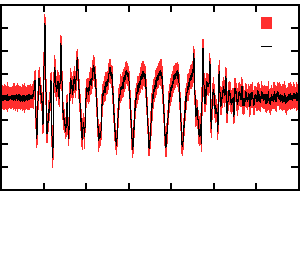
\includegraphics{voltage_0_088_gap_between_pulses_100_no_imaging_av_with_sd_means1_large}}%
    \gplfronttext
  \end{picture}%
\endgroup

    \label{fig:exp:control:av:pressure:088:first}}
 \quad
  \subfloat[2nd pulse - \pEE]{
    \label{fig:exp:control:av:pressure:088:second}
    % GNUPLOT: LaTeX picture with Postscript
\begingroup
  \makeatletter
  \providecommand\color[2][]{%
    \GenericError{(gnuplot) \space\space\space\@spaces}{%
      Package color not loaded in conjunction with
      terminal option `colourtext'%
    }{See the gnuplot documentation for explanation.%
    }{Either use 'blacktext' in gnuplot or load the package
      color.sty in LaTeX.}%
    \renewcommand\color[2][]{}%
  }%
  \providecommand\includegraphics[2][]{%
    \GenericError{(gnuplot) \space\space\space\@spaces}{%
      Package graphicx or graphics not loaded%
    }{See the gnuplot documentation for explanation.%
    }{The gnuplot epslatex terminal needs graphicx.sty or graphics.sty.}%
    \renewcommand\includegraphics[2][]{}%
  }%
  \providecommand\rotatebox[2]{#2}%
  \@ifundefined{ifGPcolor}{%
    \newif\ifGPcolor
    \GPcolortrue
  }{}%
  \@ifundefined{ifGPblacktext}{%
    \newif\ifGPblacktext
    \GPblacktexttrue
  }{}%
  % define a \g@addto@macro without @ in the name:
  \let\gplgaddtomacro\g@addto@macro
  % define empty templates for all commands taking text:
  \gdef\gplbacktext{}%
  \gdef\gplfronttext{}%
  \makeatother
  \ifGPblacktext
    % no textcolor at all
    \def\colorrgb#1{}%
    \def\colorgray#1{}%
  \else
    % gray or color?
    \ifGPcolor
      \def\colorrgb#1{\color[rgb]{#1}}%
      \def\colorgray#1{\color[gray]{#1}}%
      \expandafter\def\csname LTw\endcsname{\color{white}}%
      \expandafter\def\csname LTb\endcsname{\color{black}}%
      \expandafter\def\csname LTa\endcsname{\color{black}}%
      \expandafter\def\csname LT0\endcsname{\color[rgb]{1,0,0}}%
      \expandafter\def\csname LT1\endcsname{\color[rgb]{0,1,0}}%
      \expandafter\def\csname LT2\endcsname{\color[rgb]{0,0,1}}%
      \expandafter\def\csname LT3\endcsname{\color[rgb]{1,0,1}}%
      \expandafter\def\csname LT4\endcsname{\color[rgb]{0,1,1}}%
      \expandafter\def\csname LT5\endcsname{\color[rgb]{1,1,0}}%
      \expandafter\def\csname LT6\endcsname{\color[rgb]{0,0,0}}%
      \expandafter\def\csname LT7\endcsname{\color[rgb]{1,0.3,0}}%
      \expandafter\def\csname LT8\endcsname{\color[rgb]{0.5,0.5,0.5}}%
    \else
      % gray
      \def\colorrgb#1{\color{black}}%
      \def\colorgray#1{\color[gray]{#1}}%
      \expandafter\def\csname LTw\endcsname{\color{white}}%
      \expandafter\def\csname LTb\endcsname{\color{black}}%
      \expandafter\def\csname LTa\endcsname{\color{black}}%
      \expandafter\def\csname LT0\endcsname{\color{black}}%
      \expandafter\def\csname LT1\endcsname{\color{black}}%
      \expandafter\def\csname LT2\endcsname{\color{black}}%
      \expandafter\def\csname LT3\endcsname{\color{black}}%
      \expandafter\def\csname LT4\endcsname{\color{black}}%
      \expandafter\def\csname LT5\endcsname{\color{black}}%
      \expandafter\def\csname LT6\endcsname{\color{black}}%
      \expandafter\def\csname LT7\endcsname{\color{black}}%
      \expandafter\def\csname LT8\endcsname{\color{black}}%
    \fi
  \fi
  \setlength{\unitlength}{0.0500bp}%
  \begin{picture}(2880.00,2520.00)%
    \gplgaddtomacro\gplbacktext{%
      \csname LTb\endcsname%
      \put(-119,704){\makebox(0,0)[r]{\strut{}}}%
      \put(-119,999){\makebox(0,0)[r]{\strut{}}}%
      \put(-119,1295){\makebox(0,0)[r]{\strut{}}}%
      \put(-119,1590){\makebox(0,0)[r]{\strut{}}}%
      \put(-119,1885){\makebox(0,0)[r]{\strut{}}}%
      \put(-119,2181){\makebox(0,0)[r]{\strut{}}}%
      \put(-119,2476){\makebox(0,0)[r]{\strut{}}}%
      \put(13,484){\makebox(0,0){\strut{} 0}}%
      \put(421,484){\makebox(0,0){\strut{} 5}}%
      \put(828,484){\makebox(0,0){\strut{} 10}}%
      \put(1236,484){\makebox(0,0){\strut{} 15}}%
      \put(1643,484){\makebox(0,0){\strut{} 20}}%
      \put(2051,484){\makebox(0,0){\strut{} 25}}%
      \put(2458,484){\makebox(0,0){\strut{} 30}}%
      \put(2866,484){\makebox(0,0){\strut{} 35}}%
      \put(1439,154){\makebox(0,0){\strut{}time ($\mu$ s)}}%
    }%
    \gplgaddtomacro\gplfronttext{%
      \csname LTb\endcsname%
      \put(2381,2303){\makebox(0,0)[r]{\strut{}1-$\sigma$}}%
      \csname LTb\endcsname%
      \put(2381,2083){\makebox(0,0)[r]{\strut{}av.}}%
    }%
    \gplbacktext
    \put(0,0){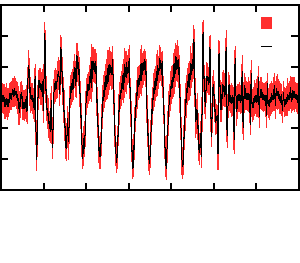
\includegraphics{voltage_0_088_gap_between_pulses_100_no_imaging_av_with_sd_means2_large}}%
    \gplfronttext
  \end{picture}%
\endgroup
}\\
  \subfloat[1st pulse - \pOOE]{
    \label{fig:exp:control:av:pressure:108:first}
    % GNUPLOT: LaTeX picture with Postscript
\begingroup
  \makeatletter
  \providecommand\color[2][]{%
    \GenericError{(gnuplot) \space\space\space\@spaces}{%
      Package color not loaded in conjunction with
      terminal option `colourtext'%
    }{See the gnuplot documentation for explanation.%
    }{Either use 'blacktext' in gnuplot or load the package
      color.sty in LaTeX.}%
    \renewcommand\color[2][]{}%
  }%
  \providecommand\includegraphics[2][]{%
    \GenericError{(gnuplot) \space\space\space\@spaces}{%
      Package graphicx or graphics not loaded%
    }{See the gnuplot documentation for explanation.%
    }{The gnuplot epslatex terminal needs graphicx.sty or graphics.sty.}%
    \renewcommand\includegraphics[2][]{}%
  }%
  \providecommand\rotatebox[2]{#2}%
  \@ifundefined{ifGPcolor}{%
    \newif\ifGPcolor
    \GPcolortrue
  }{}%
  \@ifundefined{ifGPblacktext}{%
    \newif\ifGPblacktext
    \GPblacktexttrue
  }{}%
  % define a \g@addto@macro without @ in the name:
  \let\gplgaddtomacro\g@addto@macro
  % define empty templates for all commands taking text:
  \gdef\gplbacktext{}%
  \gdef\gplfronttext{}%
  \makeatother
  \ifGPblacktext
    % no textcolor at all
    \def\colorrgb#1{}%
    \def\colorgray#1{}%
  \else
    % gray or color?
    \ifGPcolor
      \def\colorrgb#1{\color[rgb]{#1}}%
      \def\colorgray#1{\color[gray]{#1}}%
      \expandafter\def\csname LTw\endcsname{\color{white}}%
      \expandafter\def\csname LTb\endcsname{\color{black}}%
      \expandafter\def\csname LTa\endcsname{\color{black}}%
      \expandafter\def\csname LT0\endcsname{\color[rgb]{1,0,0}}%
      \expandafter\def\csname LT1\endcsname{\color[rgb]{0,1,0}}%
      \expandafter\def\csname LT2\endcsname{\color[rgb]{0,0,1}}%
      \expandafter\def\csname LT3\endcsname{\color[rgb]{1,0,1}}%
      \expandafter\def\csname LT4\endcsname{\color[rgb]{0,1,1}}%
      \expandafter\def\csname LT5\endcsname{\color[rgb]{1,1,0}}%
      \expandafter\def\csname LT6\endcsname{\color[rgb]{0,0,0}}%
      \expandafter\def\csname LT7\endcsname{\color[rgb]{1,0.3,0}}%
      \expandafter\def\csname LT8\endcsname{\color[rgb]{0.5,0.5,0.5}}%
    \else
      % gray
      \def\colorrgb#1{\color{black}}%
      \def\colorgray#1{\color[gray]{#1}}%
      \expandafter\def\csname LTw\endcsname{\color{white}}%
      \expandafter\def\csname LTb\endcsname{\color{black}}%
      \expandafter\def\csname LTa\endcsname{\color{black}}%
      \expandafter\def\csname LT0\endcsname{\color{black}}%
      \expandafter\def\csname LT1\endcsname{\color{black}}%
      \expandafter\def\csname LT2\endcsname{\color{black}}%
      \expandafter\def\csname LT3\endcsname{\color{black}}%
      \expandafter\def\csname LT4\endcsname{\color{black}}%
      \expandafter\def\csname LT5\endcsname{\color{black}}%
      \expandafter\def\csname LT6\endcsname{\color{black}}%
      \expandafter\def\csname LT7\endcsname{\color{black}}%
      \expandafter\def\csname LT8\endcsname{\color{black}}%
    \fi
  \fi
  \setlength{\unitlength}{0.0500bp}%
  \begin{picture}(2880.00,2520.00)%
    \gplgaddtomacro\gplbacktext{%
      \csname LTb\endcsname%
      \put(-119,782){\makebox(0,0)[r]{\strut{}-1}}%
      \put(-119,1040){\makebox(0,0)[r]{\strut{}-0.5}}%
      \put(-119,1298){\makebox(0,0)[r]{\strut{} 0}}%
      \put(-119,1556){\makebox(0,0)[r]{\strut{} 0.5}}%
      \put(-119,1814){\makebox(0,0)[r]{\strut{} 1}}%
      \put(-119,2072){\makebox(0,0)[r]{\strut{} 1.5}}%
      \put(-119,2330){\makebox(0,0)[r]{\strut{} 2}}%
      \put(13,484){\makebox(0,0){\strut{} 0}}%
      \put(421,484){\makebox(0,0){\strut{} 5}}%
      \put(828,484){\makebox(0,0){\strut{} 10}}%
      \put(1236,484){\makebox(0,0){\strut{} 15}}%
      \put(1643,484){\makebox(0,0){\strut{} 20}}%
      \put(2051,484){\makebox(0,0){\strut{} 25}}%
      \put(2458,484){\makebox(0,0){\strut{} 30}}%
      \put(2866,484){\makebox(0,0){\strut{} 35}}%
      \put(-889,1590){\rotatebox{-270}{\makebox(0,0){\strut{}voltage (V)}}}%
      \put(1439,154){\makebox(0,0){\strut{}time ($\mu$ s)}}%
    }%
    \gplgaddtomacro\gplfronttext{%
      \csname LTb\endcsname%
      \put(2381,2303){\makebox(0,0)[r]{\strut{}1-$\sigma$}}%
      \csname LTb\endcsname%
      \put(2381,2083){\makebox(0,0)[r]{\strut{}av.}}%
    }%
    \gplbacktext
    \put(0,0){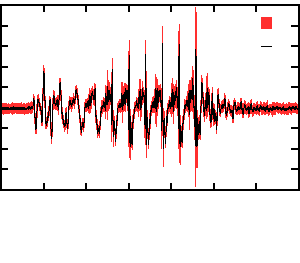
\includegraphics{voltage_0_108_gap_between_pulses_100_no_imaging_av_with_sd_means1_large}}%
    \gplfronttext
  \end{picture}%
\endgroup
}
 \quad
  \subfloat[2nd pulse - \pOOE]{
    \label{fig:exp:control:av:pressure:108:second}
    % GNUPLOT: LaTeX picture with Postscript
\begingroup
  \makeatletter
  \providecommand\color[2][]{%
    \GenericError{(gnuplot) \space\space\space\@spaces}{%
      Package color not loaded in conjunction with
      terminal option `colourtext'%
    }{See the gnuplot documentation for explanation.%
    }{Either use 'blacktext' in gnuplot or load the package
      color.sty in LaTeX.}%
    \renewcommand\color[2][]{}%
  }%
  \providecommand\includegraphics[2][]{%
    \GenericError{(gnuplot) \space\space\space\@spaces}{%
      Package graphicx or graphics not loaded%
    }{See the gnuplot documentation for explanation.%
    }{The gnuplot epslatex terminal needs graphicx.sty or graphics.sty.}%
    \renewcommand\includegraphics[2][]{}%
  }%
  \providecommand\rotatebox[2]{#2}%
  \@ifundefined{ifGPcolor}{%
    \newif\ifGPcolor
    \GPcolortrue
  }{}%
  \@ifundefined{ifGPblacktext}{%
    \newif\ifGPblacktext
    \GPblacktexttrue
  }{}%
  % define a \g@addto@macro without @ in the name:
  \let\gplgaddtomacro\g@addto@macro
  % define empty templates for all commands taking text:
  \gdef\gplbacktext{}%
  \gdef\gplfronttext{}%
  \makeatother
  \ifGPblacktext
    % no textcolor at all
    \def\colorrgb#1{}%
    \def\colorgray#1{}%
  \else
    % gray or color?
    \ifGPcolor
      \def\colorrgb#1{\color[rgb]{#1}}%
      \def\colorgray#1{\color[gray]{#1}}%
      \expandafter\def\csname LTw\endcsname{\color{white}}%
      \expandafter\def\csname LTb\endcsname{\color{black}}%
      \expandafter\def\csname LTa\endcsname{\color{black}}%
      \expandafter\def\csname LT0\endcsname{\color[rgb]{1,0,0}}%
      \expandafter\def\csname LT1\endcsname{\color[rgb]{0,1,0}}%
      \expandafter\def\csname LT2\endcsname{\color[rgb]{0,0,1}}%
      \expandafter\def\csname LT3\endcsname{\color[rgb]{1,0,1}}%
      \expandafter\def\csname LT4\endcsname{\color[rgb]{0,1,1}}%
      \expandafter\def\csname LT5\endcsname{\color[rgb]{1,1,0}}%
      \expandafter\def\csname LT6\endcsname{\color[rgb]{0,0,0}}%
      \expandafter\def\csname LT7\endcsname{\color[rgb]{1,0.3,0}}%
      \expandafter\def\csname LT8\endcsname{\color[rgb]{0.5,0.5,0.5}}%
    \else
      % gray
      \def\colorrgb#1{\color{black}}%
      \def\colorgray#1{\color[gray]{#1}}%
      \expandafter\def\csname LTw\endcsname{\color{white}}%
      \expandafter\def\csname LTb\endcsname{\color{black}}%
      \expandafter\def\csname LTa\endcsname{\color{black}}%
      \expandafter\def\csname LT0\endcsname{\color{black}}%
      \expandafter\def\csname LT1\endcsname{\color{black}}%
      \expandafter\def\csname LT2\endcsname{\color{black}}%
      \expandafter\def\csname LT3\endcsname{\color{black}}%
      \expandafter\def\csname LT4\endcsname{\color{black}}%
      \expandafter\def\csname LT5\endcsname{\color{black}}%
      \expandafter\def\csname LT6\endcsname{\color{black}}%
      \expandafter\def\csname LT7\endcsname{\color{black}}%
      \expandafter\def\csname LT8\endcsname{\color{black}}%
    \fi
  \fi
  \setlength{\unitlength}{0.0500bp}%
  \begin{picture}(2880.00,2520.00)%
    \gplgaddtomacro\gplbacktext{%
      \csname LTb\endcsname%
      \put(-119,704){\makebox(0,0)[r]{\strut{}}}%
      \put(-119,926){\makebox(0,0)[r]{\strut{}}}%
      \put(-119,1147){\makebox(0,0)[r]{\strut{}}}%
      \put(-119,1369){\makebox(0,0)[r]{\strut{}}}%
      \put(-119,1590){\makebox(0,0)[r]{\strut{}}}%
      \put(-119,1812){\makebox(0,0)[r]{\strut{}}}%
      \put(-119,2033){\makebox(0,0)[r]{\strut{}}}%
      \put(-119,2255){\makebox(0,0)[r]{\strut{}}}%
      \put(-119,2476){\makebox(0,0)[r]{\strut{}}}%
      \put(13,484){\makebox(0,0){\strut{} 0}}%
      \put(421,484){\makebox(0,0){\strut{} 5}}%
      \put(828,484){\makebox(0,0){\strut{} 10}}%
      \put(1236,484){\makebox(0,0){\strut{} 15}}%
      \put(1643,484){\makebox(0,0){\strut{} 20}}%
      \put(2051,484){\makebox(0,0){\strut{} 25}}%
      \put(2458,484){\makebox(0,0){\strut{} 30}}%
      \put(2866,484){\makebox(0,0){\strut{} 35}}%
      \put(1439,154){\makebox(0,0){\strut{}time ($\mu$ s)}}%
    }%
    \gplgaddtomacro\gplfronttext{%
      \csname LTb\endcsname%
      \put(2381,2303){\makebox(0,0)[r]{\strut{}1-$\sigma$}}%
      \csname LTb\endcsname%
      \put(2381,2083){\makebox(0,0)[r]{\strut{}av.}}%
    }%
    \gplbacktext
    \put(0,0){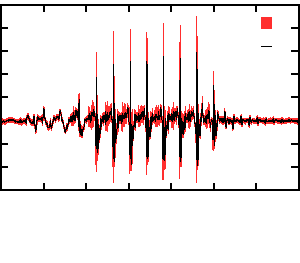
\includegraphics{voltage_0_108_gap_between_pulses_100_no_imaging_av_with_sd_means2_large}}%
    \gplfronttext
  \end{picture}%
\endgroup
}\\
  \subfloat[1st pulse - \pOTT]{
    \label{fig:exp:control:av:pressure:132:first}
    % GNUPLOT: LaTeX picture with Postscript
\begingroup
  \makeatletter
  \providecommand\color[2][]{%
    \GenericError{(gnuplot) \space\space\space\@spaces}{%
      Package color not loaded in conjunction with
      terminal option `colourtext'%
    }{See the gnuplot documentation for explanation.%
    }{Either use 'blacktext' in gnuplot or load the package
      color.sty in LaTeX.}%
    \renewcommand\color[2][]{}%
  }%
  \providecommand\includegraphics[2][]{%
    \GenericError{(gnuplot) \space\space\space\@spaces}{%
      Package graphicx or graphics not loaded%
    }{See the gnuplot documentation for explanation.%
    }{The gnuplot epslatex terminal needs graphicx.sty or graphics.sty.}%
    \renewcommand\includegraphics[2][]{}%
  }%
  \providecommand\rotatebox[2]{#2}%
  \@ifundefined{ifGPcolor}{%
    \newif\ifGPcolor
    \GPcolortrue
  }{}%
  \@ifundefined{ifGPblacktext}{%
    \newif\ifGPblacktext
    \GPblacktexttrue
  }{}%
  % define a \g@addto@macro without @ in the name:
  \let\gplgaddtomacro\g@addto@macro
  % define empty templates for all commands taking text:
  \gdef\gplbacktext{}%
  \gdef\gplfronttext{}%
  \makeatother
  \ifGPblacktext
    % no textcolor at all
    \def\colorrgb#1{}%
    \def\colorgray#1{}%
  \else
    % gray or color?
    \ifGPcolor
      \def\colorrgb#1{\color[rgb]{#1}}%
      \def\colorgray#1{\color[gray]{#1}}%
      \expandafter\def\csname LTw\endcsname{\color{white}}%
      \expandafter\def\csname LTb\endcsname{\color{black}}%
      \expandafter\def\csname LTa\endcsname{\color{black}}%
      \expandafter\def\csname LT0\endcsname{\color[rgb]{1,0,0}}%
      \expandafter\def\csname LT1\endcsname{\color[rgb]{0,1,0}}%
      \expandafter\def\csname LT2\endcsname{\color[rgb]{0,0,1}}%
      \expandafter\def\csname LT3\endcsname{\color[rgb]{1,0,1}}%
      \expandafter\def\csname LT4\endcsname{\color[rgb]{0,1,1}}%
      \expandafter\def\csname LT5\endcsname{\color[rgb]{1,1,0}}%
      \expandafter\def\csname LT6\endcsname{\color[rgb]{0,0,0}}%
      \expandafter\def\csname LT7\endcsname{\color[rgb]{1,0.3,0}}%
      \expandafter\def\csname LT8\endcsname{\color[rgb]{0.5,0.5,0.5}}%
    \else
      % gray
      \def\colorrgb#1{\color{black}}%
      \def\colorgray#1{\color[gray]{#1}}%
      \expandafter\def\csname LTw\endcsname{\color{white}}%
      \expandafter\def\csname LTb\endcsname{\color{black}}%
      \expandafter\def\csname LTa\endcsname{\color{black}}%
      \expandafter\def\csname LT0\endcsname{\color{black}}%
      \expandafter\def\csname LT1\endcsname{\color{black}}%
      \expandafter\def\csname LT2\endcsname{\color{black}}%
      \expandafter\def\csname LT3\endcsname{\color{black}}%
      \expandafter\def\csname LT4\endcsname{\color{black}}%
      \expandafter\def\csname LT5\endcsname{\color{black}}%
      \expandafter\def\csname LT6\endcsname{\color{black}}%
      \expandafter\def\csname LT7\endcsname{\color{black}}%
      \expandafter\def\csname LT8\endcsname{\color{black}}%
    \fi
  \fi
  \setlength{\unitlength}{0.0500bp}%
  \begin{picture}(2880.00,2520.00)%
    \gplgaddtomacro\gplbacktext{%
      \csname LTb\endcsname%
      \put(-119,704){\makebox(0,0)[r]{\strut{}-0.4}}%
      \put(-119,926){\makebox(0,0)[r]{\strut{}-0.3}}%
      \put(-119,1147){\makebox(0,0)[r]{\strut{}-0.2}}%
      \put(-119,1369){\makebox(0,0)[r]{\strut{}-0.1}}%
      \put(-119,1590){\makebox(0,0)[r]{\strut{} 0}}%
      \put(-119,1812){\makebox(0,0)[r]{\strut{} 0.1}}%
      \put(-119,2033){\makebox(0,0)[r]{\strut{} 0.2}}%
      \put(-119,2255){\makebox(0,0)[r]{\strut{} 0.3}}%
      \put(-119,2476){\makebox(0,0)[r]{\strut{} 0.4}}%
      \put(13,484){\makebox(0,0){\strut{} 0}}%
      \put(421,484){\makebox(0,0){\strut{} 5}}%
      \put(828,484){\makebox(0,0){\strut{} 10}}%
      \put(1236,484){\makebox(0,0){\strut{} 15}}%
      \put(1643,484){\makebox(0,0){\strut{} 20}}%
      \put(2051,484){\makebox(0,0){\strut{} 25}}%
      \put(2458,484){\makebox(0,0){\strut{} 30}}%
      \put(2866,484){\makebox(0,0){\strut{} 35}}%
      \put(-889,1590){\rotatebox{-270}{\makebox(0,0){\strut{}voltage (V)}}}%
      \put(1439,154){\makebox(0,0){\strut{}time ($\mu$ s)}}%
    }%
    \gplgaddtomacro\gplfronttext{%
      \csname LTb\endcsname%
      \put(2381,2303){\makebox(0,0)[r]{\strut{}1-$\sigma$}}%
      \csname LTb\endcsname%
      \put(2381,2083){\makebox(0,0)[r]{\strut{}av.}}%
    }%
    \gplbacktext
    \put(0,0){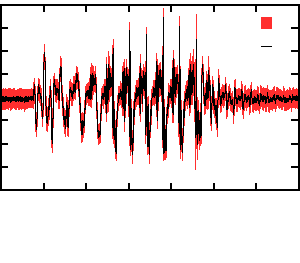
\includegraphics{voltage_0_132_gap_between_pulses_100_no_imaging_av_with_sd_means1_large}}%
    \gplfronttext
  \end{picture}%
\endgroup
}
 \quad
  \subfloat[2nd pulse - \pOTT]{
    \label{fig:exp:control:av:pressure:132:second}
    % GNUPLOT: LaTeX picture with Postscript
\begingroup
  \makeatletter
  \providecommand\color[2][]{%
    \GenericError{(gnuplot) \space\space\space\@spaces}{%
      Package color not loaded in conjunction with
      terminal option `colourtext'%
    }{See the gnuplot documentation for explanation.%
    }{Either use 'blacktext' in gnuplot or load the package
      color.sty in LaTeX.}%
    \renewcommand\color[2][]{}%
  }%
  \providecommand\includegraphics[2][]{%
    \GenericError{(gnuplot) \space\space\space\@spaces}{%
      Package graphicx or graphics not loaded%
    }{See the gnuplot documentation for explanation.%
    }{The gnuplot epslatex terminal needs graphicx.sty or graphics.sty.}%
    \renewcommand\includegraphics[2][]{}%
  }%
  \providecommand\rotatebox[2]{#2}%
  \@ifundefined{ifGPcolor}{%
    \newif\ifGPcolor
    \GPcolortrue
  }{}%
  \@ifundefined{ifGPblacktext}{%
    \newif\ifGPblacktext
    \GPblacktexttrue
  }{}%
  % define a \g@addto@macro without @ in the name:
  \let\gplgaddtomacro\g@addto@macro
  % define empty templates for all commands taking text:
  \gdef\gplbacktext{}%
  \gdef\gplfronttext{}%
  \makeatother
  \ifGPblacktext
    % no textcolor at all
    \def\colorrgb#1{}%
    \def\colorgray#1{}%
  \else
    % gray or color?
    \ifGPcolor
      \def\colorrgb#1{\color[rgb]{#1}}%
      \def\colorgray#1{\color[gray]{#1}}%
      \expandafter\def\csname LTw\endcsname{\color{white}}%
      \expandafter\def\csname LTb\endcsname{\color{black}}%
      \expandafter\def\csname LTa\endcsname{\color{black}}%
      \expandafter\def\csname LT0\endcsname{\color[rgb]{1,0,0}}%
      \expandafter\def\csname LT1\endcsname{\color[rgb]{0,1,0}}%
      \expandafter\def\csname LT2\endcsname{\color[rgb]{0,0,1}}%
      \expandafter\def\csname LT3\endcsname{\color[rgb]{1,0,1}}%
      \expandafter\def\csname LT4\endcsname{\color[rgb]{0,1,1}}%
      \expandafter\def\csname LT5\endcsname{\color[rgb]{1,1,0}}%
      \expandafter\def\csname LT6\endcsname{\color[rgb]{0,0,0}}%
      \expandafter\def\csname LT7\endcsname{\color[rgb]{1,0.3,0}}%
      \expandafter\def\csname LT8\endcsname{\color[rgb]{0.5,0.5,0.5}}%
    \else
      % gray
      \def\colorrgb#1{\color{black}}%
      \def\colorgray#1{\color[gray]{#1}}%
      \expandafter\def\csname LTw\endcsname{\color{white}}%
      \expandafter\def\csname LTb\endcsname{\color{black}}%
      \expandafter\def\csname LTa\endcsname{\color{black}}%
      \expandafter\def\csname LT0\endcsname{\color{black}}%
      \expandafter\def\csname LT1\endcsname{\color{black}}%
      \expandafter\def\csname LT2\endcsname{\color{black}}%
      \expandafter\def\csname LT3\endcsname{\color{black}}%
      \expandafter\def\csname LT4\endcsname{\color{black}}%
      \expandafter\def\csname LT5\endcsname{\color{black}}%
      \expandafter\def\csname LT6\endcsname{\color{black}}%
      \expandafter\def\csname LT7\endcsname{\color{black}}%
      \expandafter\def\csname LT8\endcsname{\color{black}}%
    \fi
  \fi
  \setlength{\unitlength}{0.0500bp}%
  \begin{picture}(2880.00,2520.00)%
    \gplgaddtomacro\gplbacktext{%
      \csname LTb\endcsname%
      \put(-119,704){\makebox(0,0)[r]{\strut{}}}%
      \put(-119,881){\makebox(0,0)[r]{\strut{}}}%
      \put(-119,1058){\makebox(0,0)[r]{\strut{}}}%
      \put(-119,1236){\makebox(0,0)[r]{\strut{}}}%
      \put(-119,1413){\makebox(0,0)[r]{\strut{}}}%
      \put(-119,1590){\makebox(0,0)[r]{\strut{}}}%
      \put(-119,1767){\makebox(0,0)[r]{\strut{}}}%
      \put(-119,1944){\makebox(0,0)[r]{\strut{}}}%
      \put(-119,2122){\makebox(0,0)[r]{\strut{}}}%
      \put(-119,2299){\makebox(0,0)[r]{\strut{}}}%
      \put(-119,2476){\makebox(0,0)[r]{\strut{}}}%
      \put(13,484){\makebox(0,0){\strut{} 0}}%
      \put(421,484){\makebox(0,0){\strut{} 5}}%
      \put(828,484){\makebox(0,0){\strut{} 10}}%
      \put(1236,484){\makebox(0,0){\strut{} 15}}%
      \put(1643,484){\makebox(0,0){\strut{} 20}}%
      \put(2051,484){\makebox(0,0){\strut{} 25}}%
      \put(2458,484){\makebox(0,0){\strut{} 30}}%
      \put(2866,484){\makebox(0,0){\strut{} 35}}%
      \put(1439,154){\makebox(0,0){\strut{}time ($\mu$ s)}}%
    }%
    \gplgaddtomacro\gplfronttext{%
      \csname LTb\endcsname%
      \put(2381,2303){\makebox(0,0)[r]{\strut{}1-$\sigma$}}%
      \csname LTb\endcsname%
      \put(2381,2083){\makebox(0,0)[r]{\strut{}av.}}%
    }%
    \gplbacktext
    \put(0,0){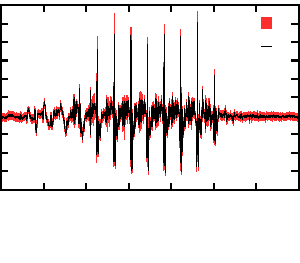
\includegraphics{voltage_0_132_gap_between_pulses_100_no_imaging_av_with_sd_means2_large}}%
    \gplfronttext
  \end{picture}%
\endgroup
}\\
  \caption{
    The pressure received  by the imaging transducer when the driving wave is on but the imaging wave is off (receive-only).
    The second pulse \subref{fig:av:108:100:second} is received \unit{100}\micro\second\ after the first \subref{fig:av:108:100:first}.
    Each image is the average of 49 images, the first standard-deviation error bars are indicated.
Three different pressures are shown below each sub-figure.
  }
  \label{fig:exp:control:av:pressure}
\end{figure}


\subsection{Control study: receive only imaging}\label{sec:exp:EP:control}

\Figref{exp:control:av:pressure} plots control data for three different pressures\todo{Pressure}.
On the left hand side (images \subref{fig:exp:control:av:pressure:088:first}, \subref{fig:exp:control:av:pressure:108:first} and
\subref{fig:exp:control:av:pressure:132:first}) shows the forward transmit received from the first pulse.
The right hand side (images \subref{fig:exp:control:av:pressure:088:second}, \subref{fig:exp:control:av:pressure:108:second} and 
\subref{fig:exp:control:av:pressure:132:second}) shows the forward transmit from the second pulse,
which occurred \unit{100}\micro\second\ after the first.

There are a number of important things to notice in \Figref{exp:control:av:pressure}:
\nlist{
\item At the higher pressures (\figref{exp:control:av:pressure:108:first}-\subref{fig:exp:control:av:pressure:132:second}) a strong and narrow response is observed over and above the more sinusoidal response found at the lower pressures  of \figref{exp:control:av:pressure:088:first} and \subref{fig:exp:control:av:pressure:088:second}.
Qualitatively \figref{exp:control:av:pressure:108:first}-\subref{fig:exp:control:av:pressure:132:second} 
bear a strong resemblance to the simulated bubble pulsations of \chapref{computations}.
The pressure dependence of these signals provide strong evidence for the generation of bubbles by the driving wave.
\item The received pressure for the first and second pulse are not the same.
In general the forward transmit from the second pulse is stronger than from the first.
This further supports the interpretation of the strong peaks in \figref{exp:control:av:pressure:108:first}-\subref{fig:exp:control:av:pressure:132:second} as forward scatter from the driving wave.
This is because the difference between the two pulses suggests a temporal lifespan of the generated bubbles of greater than the \unit{100}\micro\second\ relaxation time.
%From \figref{} this temporal dependance suggests a bubble size of more than ...\todo{get radius}
\item The noise in each image is fairly low.
  While the first and second pulse at each pressure are different,
  for each repetition of the experiment the pulses are fairly consistence.
  The indicates that after the second pulse the bubble population 
  relaxes back to its original state before the first pulse of the next test.
  The passage of an acoustic wave does not seem to fundamentally alter the sample.
}

The difference in scatter between the first and second pulse represents
both a problem and an opportunity.
It is a problem because the excess pressure method requires the  response 
of both driving wave to be the same.
It is, after all, to be subtracted away.





\begin{figure}[t]%
  \centering
  \subfloat[1st pulse - \unit{100}\micro\second]{
    \label{fig:exp:control:av:time:100:first}
    % GNUPLOT: LaTeX picture with Postscript
\begingroup
  \makeatletter
  \providecommand\color[2][]{%
    \GenericError{(gnuplot) \space\space\space\@spaces}{%
      Package color not loaded in conjunction with
      terminal option `colourtext'%
    }{See the gnuplot documentation for explanation.%
    }{Either use 'blacktext' in gnuplot or load the package
      color.sty in LaTeX.}%
    \renewcommand\color[2][]{}%
  }%
  \providecommand\includegraphics[2][]{%
    \GenericError{(gnuplot) \space\space\space\@spaces}{%
      Package graphicx or graphics not loaded%
    }{See the gnuplot documentation for explanation.%
    }{The gnuplot epslatex terminal needs graphicx.sty or graphics.sty.}%
    \renewcommand\includegraphics[2][]{}%
  }%
  \providecommand\rotatebox[2]{#2}%
  \@ifundefined{ifGPcolor}{%
    \newif\ifGPcolor
    \GPcolortrue
  }{}%
  \@ifundefined{ifGPblacktext}{%
    \newif\ifGPblacktext
    \GPblacktexttrue
  }{}%
  % define a \g@addto@macro without @ in the name:
  \let\gplgaddtomacro\g@addto@macro
  % define empty templates for all commands taking text:
  \gdef\gplbacktext{}%
  \gdef\gplfronttext{}%
  \makeatother
  \ifGPblacktext
    % no textcolor at all
    \def\colorrgb#1{}%
    \def\colorgray#1{}%
  \else
    % gray or color?
    \ifGPcolor
      \def\colorrgb#1{\color[rgb]{#1}}%
      \def\colorgray#1{\color[gray]{#1}}%
      \expandafter\def\csname LTw\endcsname{\color{white}}%
      \expandafter\def\csname LTb\endcsname{\color{black}}%
      \expandafter\def\csname LTa\endcsname{\color{black}}%
      \expandafter\def\csname LT0\endcsname{\color[rgb]{1,0,0}}%
      \expandafter\def\csname LT1\endcsname{\color[rgb]{0,1,0}}%
      \expandafter\def\csname LT2\endcsname{\color[rgb]{0,0,1}}%
      \expandafter\def\csname LT3\endcsname{\color[rgb]{1,0,1}}%
      \expandafter\def\csname LT4\endcsname{\color[rgb]{0,1,1}}%
      \expandafter\def\csname LT5\endcsname{\color[rgb]{1,1,0}}%
      \expandafter\def\csname LT6\endcsname{\color[rgb]{0,0,0}}%
      \expandafter\def\csname LT7\endcsname{\color[rgb]{1,0.3,0}}%
      \expandafter\def\csname LT8\endcsname{\color[rgb]{0.5,0.5,0.5}}%
    \else
      % gray
      \def\colorrgb#1{\color{black}}%
      \def\colorgray#1{\color[gray]{#1}}%
      \expandafter\def\csname LTw\endcsname{\color{white}}%
      \expandafter\def\csname LTb\endcsname{\color{black}}%
      \expandafter\def\csname LTa\endcsname{\color{black}}%
      \expandafter\def\csname LT0\endcsname{\color{black}}%
      \expandafter\def\csname LT1\endcsname{\color{black}}%
      \expandafter\def\csname LT2\endcsname{\color{black}}%
      \expandafter\def\csname LT3\endcsname{\color{black}}%
      \expandafter\def\csname LT4\endcsname{\color{black}}%
      \expandafter\def\csname LT5\endcsname{\color{black}}%
      \expandafter\def\csname LT6\endcsname{\color{black}}%
      \expandafter\def\csname LT7\endcsname{\color{black}}%
      \expandafter\def\csname LT8\endcsname{\color{black}}%
    \fi
  \fi
  \setlength{\unitlength}{0.0500bp}%
  \begin{picture}(2880.00,2520.00)%
    \gplgaddtomacro\gplbacktext{%
      \csname LTb\endcsname%
      \put(-119,782){\makebox(0,0)[r]{\strut{}-1}}%
      \put(-119,1040){\makebox(0,0)[r]{\strut{}-0.5}}%
      \put(-119,1298){\makebox(0,0)[r]{\strut{} 0}}%
      \put(-119,1556){\makebox(0,0)[r]{\strut{} 0.5}}%
      \put(-119,1814){\makebox(0,0)[r]{\strut{} 1}}%
      \put(-119,2072){\makebox(0,0)[r]{\strut{} 1.5}}%
      \put(-119,2330){\makebox(0,0)[r]{\strut{} 2}}%
      \put(13,484){\makebox(0,0){\strut{} 0}}%
      \put(421,484){\makebox(0,0){\strut{} 5}}%
      \put(828,484){\makebox(0,0){\strut{} 10}}%
      \put(1236,484){\makebox(0,0){\strut{} 15}}%
      \put(1643,484){\makebox(0,0){\strut{} 20}}%
      \put(2051,484){\makebox(0,0){\strut{} 25}}%
      \put(2458,484){\makebox(0,0){\strut{} 30}}%
      \put(2866,484){\makebox(0,0){\strut{} 35}}%
      \put(-889,1590){\rotatebox{-270}{\makebox(0,0){\strut{}voltage (V)}}}%
      \put(1439,154){\makebox(0,0){\strut{}time ($\mu$ s)}}%
    }%
    \gplgaddtomacro\gplfronttext{%
      \csname LTb\endcsname%
      \put(2381,2303){\makebox(0,0)[r]{\strut{}1-$\sigma$}}%
      \csname LTb\endcsname%
      \put(2381,2083){\makebox(0,0)[r]{\strut{}av.}}%
    }%
    \gplbacktext
    \put(0,0){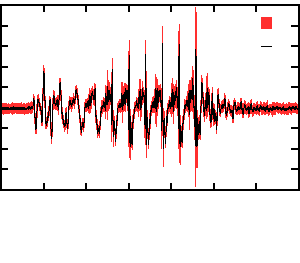
\includegraphics{voltage_0_108_gap_between_pulses_100_no_imaging_av_with_sd_means1_large}}%
    \gplfronttext
  \end{picture}%
\endgroup
}
 \quad
  \subfloat[2nd pulse - \unit{100}\micro\second]{
    \label{fig:exp:control:av:time:100:second}
    % GNUPLOT: LaTeX picture with Postscript
\begingroup
  \makeatletter
  \providecommand\color[2][]{%
    \GenericError{(gnuplot) \space\space\space\@spaces}{%
      Package color not loaded in conjunction with
      terminal option `colourtext'%
    }{See the gnuplot documentation for explanation.%
    }{Either use 'blacktext' in gnuplot or load the package
      color.sty in LaTeX.}%
    \renewcommand\color[2][]{}%
  }%
  \providecommand\includegraphics[2][]{%
    \GenericError{(gnuplot) \space\space\space\@spaces}{%
      Package graphicx or graphics not loaded%
    }{See the gnuplot documentation for explanation.%
    }{The gnuplot epslatex terminal needs graphicx.sty or graphics.sty.}%
    \renewcommand\includegraphics[2][]{}%
  }%
  \providecommand\rotatebox[2]{#2}%
  \@ifundefined{ifGPcolor}{%
    \newif\ifGPcolor
    \GPcolortrue
  }{}%
  \@ifundefined{ifGPblacktext}{%
    \newif\ifGPblacktext
    \GPblacktexttrue
  }{}%
  % define a \g@addto@macro without @ in the name:
  \let\gplgaddtomacro\g@addto@macro
  % define empty templates for all commands taking text:
  \gdef\gplbacktext{}%
  \gdef\gplfronttext{}%
  \makeatother
  \ifGPblacktext
    % no textcolor at all
    \def\colorrgb#1{}%
    \def\colorgray#1{}%
  \else
    % gray or color?
    \ifGPcolor
      \def\colorrgb#1{\color[rgb]{#1}}%
      \def\colorgray#1{\color[gray]{#1}}%
      \expandafter\def\csname LTw\endcsname{\color{white}}%
      \expandafter\def\csname LTb\endcsname{\color{black}}%
      \expandafter\def\csname LTa\endcsname{\color{black}}%
      \expandafter\def\csname LT0\endcsname{\color[rgb]{1,0,0}}%
      \expandafter\def\csname LT1\endcsname{\color[rgb]{0,1,0}}%
      \expandafter\def\csname LT2\endcsname{\color[rgb]{0,0,1}}%
      \expandafter\def\csname LT3\endcsname{\color[rgb]{1,0,1}}%
      \expandafter\def\csname LT4\endcsname{\color[rgb]{0,1,1}}%
      \expandafter\def\csname LT5\endcsname{\color[rgb]{1,1,0}}%
      \expandafter\def\csname LT6\endcsname{\color[rgb]{0,0,0}}%
      \expandafter\def\csname LT7\endcsname{\color[rgb]{1,0.3,0}}%
      \expandafter\def\csname LT8\endcsname{\color[rgb]{0.5,0.5,0.5}}%
    \else
      % gray
      \def\colorrgb#1{\color{black}}%
      \def\colorgray#1{\color[gray]{#1}}%
      \expandafter\def\csname LTw\endcsname{\color{white}}%
      \expandafter\def\csname LTb\endcsname{\color{black}}%
      \expandafter\def\csname LTa\endcsname{\color{black}}%
      \expandafter\def\csname LT0\endcsname{\color{black}}%
      \expandafter\def\csname LT1\endcsname{\color{black}}%
      \expandafter\def\csname LT2\endcsname{\color{black}}%
      \expandafter\def\csname LT3\endcsname{\color{black}}%
      \expandafter\def\csname LT4\endcsname{\color{black}}%
      \expandafter\def\csname LT5\endcsname{\color{black}}%
      \expandafter\def\csname LT6\endcsname{\color{black}}%
      \expandafter\def\csname LT7\endcsname{\color{black}}%
      \expandafter\def\csname LT8\endcsname{\color{black}}%
    \fi
  \fi
  \setlength{\unitlength}{0.0500bp}%
  \begin{picture}(2880.00,2520.00)%
    \gplgaddtomacro\gplbacktext{%
      \csname LTb\endcsname%
      \put(-119,704){\makebox(0,0)[r]{\strut{}}}%
      \put(-119,926){\makebox(0,0)[r]{\strut{}}}%
      \put(-119,1147){\makebox(0,0)[r]{\strut{}}}%
      \put(-119,1369){\makebox(0,0)[r]{\strut{}}}%
      \put(-119,1590){\makebox(0,0)[r]{\strut{}}}%
      \put(-119,1812){\makebox(0,0)[r]{\strut{}}}%
      \put(-119,2033){\makebox(0,0)[r]{\strut{}}}%
      \put(-119,2255){\makebox(0,0)[r]{\strut{}}}%
      \put(-119,2476){\makebox(0,0)[r]{\strut{}}}%
      \put(13,484){\makebox(0,0){\strut{} 0}}%
      \put(421,484){\makebox(0,0){\strut{} 5}}%
      \put(828,484){\makebox(0,0){\strut{} 10}}%
      \put(1236,484){\makebox(0,0){\strut{} 15}}%
      \put(1643,484){\makebox(0,0){\strut{} 20}}%
      \put(2051,484){\makebox(0,0){\strut{} 25}}%
      \put(2458,484){\makebox(0,0){\strut{} 30}}%
      \put(2866,484){\makebox(0,0){\strut{} 35}}%
      \put(1439,154){\makebox(0,0){\strut{}time ($\mu$ s)}}%
    }%
    \gplgaddtomacro\gplfronttext{%
      \csname LTb\endcsname%
      \put(2381,2303){\makebox(0,0)[r]{\strut{}1-$\sigma$}}%
      \csname LTb\endcsname%
      \put(2381,2083){\makebox(0,0)[r]{\strut{}av.}}%
    }%
    \gplbacktext
    \put(0,0){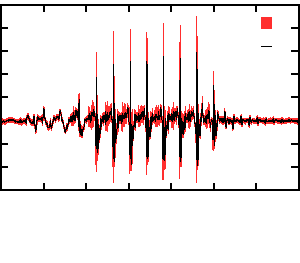
\includegraphics{voltage_0_108_gap_between_pulses_100_no_imaging_av_with_sd_means2_large}}%
    \gplfronttext
  \end{picture}%
\endgroup
}\\
  \subfloat[1st pulse - \unit{150}\micro\second]{
    \label{fig:exp:control:av:time:150:first}
    % GNUPLOT: LaTeX picture with Postscript
\begingroup
  \makeatletter
  \providecommand\color[2][]{%
    \GenericError{(gnuplot) \space\space\space\@spaces}{%
      Package color not loaded in conjunction with
      terminal option `colourtext'%
    }{See the gnuplot documentation for explanation.%
    }{Either use 'blacktext' in gnuplot or load the package
      color.sty in LaTeX.}%
    \renewcommand\color[2][]{}%
  }%
  \providecommand\includegraphics[2][]{%
    \GenericError{(gnuplot) \space\space\space\@spaces}{%
      Package graphicx or graphics not loaded%
    }{See the gnuplot documentation for explanation.%
    }{The gnuplot epslatex terminal needs graphicx.sty or graphics.sty.}%
    \renewcommand\includegraphics[2][]{}%
  }%
  \providecommand\rotatebox[2]{#2}%
  \@ifundefined{ifGPcolor}{%
    \newif\ifGPcolor
    \GPcolortrue
  }{}%
  \@ifundefined{ifGPblacktext}{%
    \newif\ifGPblacktext
    \GPblacktexttrue
  }{}%
  % define a \g@addto@macro without @ in the name:
  \let\gplgaddtomacro\g@addto@macro
  % define empty templates for all commands taking text:
  \gdef\gplbacktext{}%
  \gdef\gplfronttext{}%
  \makeatother
  \ifGPblacktext
    % no textcolor at all
    \def\colorrgb#1{}%
    \def\colorgray#1{}%
  \else
    % gray or color?
    \ifGPcolor
      \def\colorrgb#1{\color[rgb]{#1}}%
      \def\colorgray#1{\color[gray]{#1}}%
      \expandafter\def\csname LTw\endcsname{\color{white}}%
      \expandafter\def\csname LTb\endcsname{\color{black}}%
      \expandafter\def\csname LTa\endcsname{\color{black}}%
      \expandafter\def\csname LT0\endcsname{\color[rgb]{1,0,0}}%
      \expandafter\def\csname LT1\endcsname{\color[rgb]{0,1,0}}%
      \expandafter\def\csname LT2\endcsname{\color[rgb]{0,0,1}}%
      \expandafter\def\csname LT3\endcsname{\color[rgb]{1,0,1}}%
      \expandafter\def\csname LT4\endcsname{\color[rgb]{0,1,1}}%
      \expandafter\def\csname LT5\endcsname{\color[rgb]{1,1,0}}%
      \expandafter\def\csname LT6\endcsname{\color[rgb]{0,0,0}}%
      \expandafter\def\csname LT7\endcsname{\color[rgb]{1,0.3,0}}%
      \expandafter\def\csname LT8\endcsname{\color[rgb]{0.5,0.5,0.5}}%
    \else
      % gray
      \def\colorrgb#1{\color{black}}%
      \def\colorgray#1{\color[gray]{#1}}%
      \expandafter\def\csname LTw\endcsname{\color{white}}%
      \expandafter\def\csname LTb\endcsname{\color{black}}%
      \expandafter\def\csname LTa\endcsname{\color{black}}%
      \expandafter\def\csname LT0\endcsname{\color{black}}%
      \expandafter\def\csname LT1\endcsname{\color{black}}%
      \expandafter\def\csname LT2\endcsname{\color{black}}%
      \expandafter\def\csname LT3\endcsname{\color{black}}%
      \expandafter\def\csname LT4\endcsname{\color{black}}%
      \expandafter\def\csname LT5\endcsname{\color{black}}%
      \expandafter\def\csname LT6\endcsname{\color{black}}%
      \expandafter\def\csname LT7\endcsname{\color{black}}%
      \expandafter\def\csname LT8\endcsname{\color{black}}%
    \fi
  \fi
  \setlength{\unitlength}{0.0500bp}%
  \begin{picture}(2880.00,2520.00)%
    \gplgaddtomacro\gplbacktext{%
      \csname LTb\endcsname%
      \put(-119,704){\makebox(0,0)[r]{\strut{}-0.6}}%
      \put(-119,957){\makebox(0,0)[r]{\strut{}-0.4}}%
      \put(-119,1210){\makebox(0,0)[r]{\strut{}-0.2}}%
      \put(-119,1463){\makebox(0,0)[r]{\strut{} 0}}%
      \put(-119,1717){\makebox(0,0)[r]{\strut{} 0.2}}%
      \put(-119,1970){\makebox(0,0)[r]{\strut{} 0.4}}%
      \put(-119,2223){\makebox(0,0)[r]{\strut{} 0.6}}%
      \put(-119,2476){\makebox(0,0)[r]{\strut{} 0.8}}%
      \put(13,484){\makebox(0,0){\strut{} 0}}%
      \put(421,484){\makebox(0,0){\strut{} 5}}%
      \put(828,484){\makebox(0,0){\strut{} 10}}%
      \put(1236,484){\makebox(0,0){\strut{} 15}}%
      \put(1643,484){\makebox(0,0){\strut{} 20}}%
      \put(2051,484){\makebox(0,0){\strut{} 25}}%
      \put(2458,484){\makebox(0,0){\strut{} 30}}%
      \put(2866,484){\makebox(0,0){\strut{} 35}}%
      \put(-889,1590){\rotatebox{-270}{\makebox(0,0){\strut{}voltage (V)}}}%
      \put(1439,154){\makebox(0,0){\strut{}time ($\mu$ s)}}%
    }%
    \gplgaddtomacro\gplfronttext{%
      \csname LTb\endcsname%
      \put(2381,2303){\makebox(0,0)[r]{\strut{}1-$\sigma$}}%
      \csname LTb\endcsname%
      \put(2381,2083){\makebox(0,0)[r]{\strut{}av.}}%
    }%
    \gplbacktext
    \put(0,0){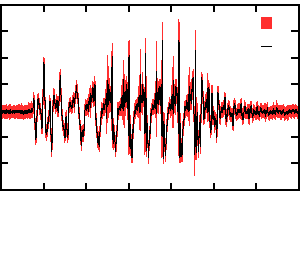
\includegraphics{voltage_0_108_gap_between_pulses_150_no_imaging_av_with_sd_means1_large}}%
    \gplfronttext
  \end{picture}%
\endgroup
}
 \quad
  \subfloat[2nd pulse - \unit{150}\micro\second]{
    \label{fig:exp:control:av:time:150:second}
    % GNUPLOT: LaTeX picture with Postscript
\begingroup
  \makeatletter
  \providecommand\color[2][]{%
    \GenericError{(gnuplot) \space\space\space\@spaces}{%
      Package color not loaded in conjunction with
      terminal option `colourtext'%
    }{See the gnuplot documentation for explanation.%
    }{Either use 'blacktext' in gnuplot or load the package
      color.sty in LaTeX.}%
    \renewcommand\color[2][]{}%
  }%
  \providecommand\includegraphics[2][]{%
    \GenericError{(gnuplot) \space\space\space\@spaces}{%
      Package graphicx or graphics not loaded%
    }{See the gnuplot documentation for explanation.%
    }{The gnuplot epslatex terminal needs graphicx.sty or graphics.sty.}%
    \renewcommand\includegraphics[2][]{}%
  }%
  \providecommand\rotatebox[2]{#2}%
  \@ifundefined{ifGPcolor}{%
    \newif\ifGPcolor
    \GPcolortrue
  }{}%
  \@ifundefined{ifGPblacktext}{%
    \newif\ifGPblacktext
    \GPblacktexttrue
  }{}%
  % define a \g@addto@macro without @ in the name:
  \let\gplgaddtomacro\g@addto@macro
  % define empty templates for all commands taking text:
  \gdef\gplbacktext{}%
  \gdef\gplfronttext{}%
  \makeatother
  \ifGPblacktext
    % no textcolor at all
    \def\colorrgb#1{}%
    \def\colorgray#1{}%
  \else
    % gray or color?
    \ifGPcolor
      \def\colorrgb#1{\color[rgb]{#1}}%
      \def\colorgray#1{\color[gray]{#1}}%
      \expandafter\def\csname LTw\endcsname{\color{white}}%
      \expandafter\def\csname LTb\endcsname{\color{black}}%
      \expandafter\def\csname LTa\endcsname{\color{black}}%
      \expandafter\def\csname LT0\endcsname{\color[rgb]{1,0,0}}%
      \expandafter\def\csname LT1\endcsname{\color[rgb]{0,1,0}}%
      \expandafter\def\csname LT2\endcsname{\color[rgb]{0,0,1}}%
      \expandafter\def\csname LT3\endcsname{\color[rgb]{1,0,1}}%
      \expandafter\def\csname LT4\endcsname{\color[rgb]{0,1,1}}%
      \expandafter\def\csname LT5\endcsname{\color[rgb]{1,1,0}}%
      \expandafter\def\csname LT6\endcsname{\color[rgb]{0,0,0}}%
      \expandafter\def\csname LT7\endcsname{\color[rgb]{1,0.3,0}}%
      \expandafter\def\csname LT8\endcsname{\color[rgb]{0.5,0.5,0.5}}%
    \else
      % gray
      \def\colorrgb#1{\color{black}}%
      \def\colorgray#1{\color[gray]{#1}}%
      \expandafter\def\csname LTw\endcsname{\color{white}}%
      \expandafter\def\csname LTb\endcsname{\color{black}}%
      \expandafter\def\csname LTa\endcsname{\color{black}}%
      \expandafter\def\csname LT0\endcsname{\color{black}}%
      \expandafter\def\csname LT1\endcsname{\color{black}}%
      \expandafter\def\csname LT2\endcsname{\color{black}}%
      \expandafter\def\csname LT3\endcsname{\color{black}}%
      \expandafter\def\csname LT4\endcsname{\color{black}}%
      \expandafter\def\csname LT5\endcsname{\color{black}}%
      \expandafter\def\csname LT6\endcsname{\color{black}}%
      \expandafter\def\csname LT7\endcsname{\color{black}}%
      \expandafter\def\csname LT8\endcsname{\color{black}}%
    \fi
  \fi
  \setlength{\unitlength}{0.0500bp}%
  \begin{picture}(2880.00,2520.00)%
    \gplgaddtomacro\gplbacktext{%
      \csname LTb\endcsname%
      \put(-119,704){\makebox(0,0)[r]{\strut{}}}%
      \put(-119,901){\makebox(0,0)[r]{\strut{}}}%
      \put(-119,1098){\makebox(0,0)[r]{\strut{}}}%
      \put(-119,1295){\makebox(0,0)[r]{\strut{}}}%
      \put(-119,1492){\makebox(0,0)[r]{\strut{}}}%
      \put(-119,1688){\makebox(0,0)[r]{\strut{}}}%
      \put(-119,1885){\makebox(0,0)[r]{\strut{}}}%
      \put(-119,2082){\makebox(0,0)[r]{\strut{}}}%
      \put(-119,2279){\makebox(0,0)[r]{\strut{}}}%
      \put(-119,2476){\makebox(0,0)[r]{\strut{}}}%
      \put(13,484){\makebox(0,0){\strut{} 0}}%
      \put(421,484){\makebox(0,0){\strut{} 5}}%
      \put(828,484){\makebox(0,0){\strut{} 10}}%
      \put(1236,484){\makebox(0,0){\strut{} 15}}%
      \put(1643,484){\makebox(0,0){\strut{} 20}}%
      \put(2051,484){\makebox(0,0){\strut{} 25}}%
      \put(2458,484){\makebox(0,0){\strut{} 30}}%
      \put(2866,484){\makebox(0,0){\strut{} 35}}%
      \put(1439,154){\makebox(0,0){\strut{}time ($\mu$ s)}}%
    }%
    \gplgaddtomacro\gplfronttext{%
      \csname LTb\endcsname%
      \put(2381,2303){\makebox(0,0)[r]{\strut{}1-$\sigma$}}%
      \csname LTb\endcsname%
      \put(2381,2083){\makebox(0,0)[r]{\strut{}av.}}%
    }%
    \gplbacktext
    \put(0,0){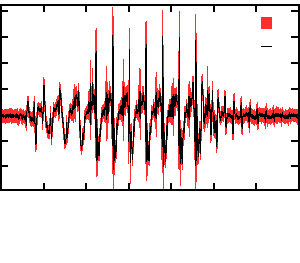
\includegraphics{voltage_0_108_gap_between_pulses_150_no_imaging_av_with_sd_means2_large}}%
    \gplfronttext
  \end{picture}%
\endgroup
}\\
  \subfloat[1st pulse - \unit{250}\micro\second]{
    \label{fig:exp:control:av:time:250:first}
    % GNUPLOT: LaTeX picture with Postscript
\begingroup
  \makeatletter
  \providecommand\color[2][]{%
    \GenericError{(gnuplot) \space\space\space\@spaces}{%
      Package color not loaded in conjunction with
      terminal option `colourtext'%
    }{See the gnuplot documentation for explanation.%
    }{Either use 'blacktext' in gnuplot or load the package
      color.sty in LaTeX.}%
    \renewcommand\color[2][]{}%
  }%
  \providecommand\includegraphics[2][]{%
    \GenericError{(gnuplot) \space\space\space\@spaces}{%
      Package graphicx or graphics not loaded%
    }{See the gnuplot documentation for explanation.%
    }{The gnuplot epslatex terminal needs graphicx.sty or graphics.sty.}%
    \renewcommand\includegraphics[2][]{}%
  }%
  \providecommand\rotatebox[2]{#2}%
  \@ifundefined{ifGPcolor}{%
    \newif\ifGPcolor
    \GPcolortrue
  }{}%
  \@ifundefined{ifGPblacktext}{%
    \newif\ifGPblacktext
    \GPblacktexttrue
  }{}%
  % define a \g@addto@macro without @ in the name:
  \let\gplgaddtomacro\g@addto@macro
  % define empty templates for all commands taking text:
  \gdef\gplbacktext{}%
  \gdef\gplfronttext{}%
  \makeatother
  \ifGPblacktext
    % no textcolor at all
    \def\colorrgb#1{}%
    \def\colorgray#1{}%
  \else
    % gray or color?
    \ifGPcolor
      \def\colorrgb#1{\color[rgb]{#1}}%
      \def\colorgray#1{\color[gray]{#1}}%
      \expandafter\def\csname LTw\endcsname{\color{white}}%
      \expandafter\def\csname LTb\endcsname{\color{black}}%
      \expandafter\def\csname LTa\endcsname{\color{black}}%
      \expandafter\def\csname LT0\endcsname{\color[rgb]{1,0,0}}%
      \expandafter\def\csname LT1\endcsname{\color[rgb]{0,1,0}}%
      \expandafter\def\csname LT2\endcsname{\color[rgb]{0,0,1}}%
      \expandafter\def\csname LT3\endcsname{\color[rgb]{1,0,1}}%
      \expandafter\def\csname LT4\endcsname{\color[rgb]{0,1,1}}%
      \expandafter\def\csname LT5\endcsname{\color[rgb]{1,1,0}}%
      \expandafter\def\csname LT6\endcsname{\color[rgb]{0,0,0}}%
      \expandafter\def\csname LT7\endcsname{\color[rgb]{1,0.3,0}}%
      \expandafter\def\csname LT8\endcsname{\color[rgb]{0.5,0.5,0.5}}%
    \else
      % gray
      \def\colorrgb#1{\color{black}}%
      \def\colorgray#1{\color[gray]{#1}}%
      \expandafter\def\csname LTw\endcsname{\color{white}}%
      \expandafter\def\csname LTb\endcsname{\color{black}}%
      \expandafter\def\csname LTa\endcsname{\color{black}}%
      \expandafter\def\csname LT0\endcsname{\color{black}}%
      \expandafter\def\csname LT1\endcsname{\color{black}}%
      \expandafter\def\csname LT2\endcsname{\color{black}}%
      \expandafter\def\csname LT3\endcsname{\color{black}}%
      \expandafter\def\csname LT4\endcsname{\color{black}}%
      \expandafter\def\csname LT5\endcsname{\color{black}}%
      \expandafter\def\csname LT6\endcsname{\color{black}}%
      \expandafter\def\csname LT7\endcsname{\color{black}}%
      \expandafter\def\csname LT8\endcsname{\color{black}}%
    \fi
  \fi
  \setlength{\unitlength}{0.0500bp}%
  \begin{picture}(2880.00,2520.00)%
    \gplgaddtomacro\gplbacktext{%
      \csname LTb\endcsname%
      \put(-119,704){\makebox(0,0)[r]{\strut{}-0.6}}%
      \put(-119,957){\makebox(0,0)[r]{\strut{}-0.4}}%
      \put(-119,1210){\makebox(0,0)[r]{\strut{}-0.2}}%
      \put(-119,1463){\makebox(0,0)[r]{\strut{} 0}}%
      \put(-119,1717){\makebox(0,0)[r]{\strut{} 0.2}}%
      \put(-119,1970){\makebox(0,0)[r]{\strut{} 0.4}}%
      \put(-119,2223){\makebox(0,0)[r]{\strut{} 0.6}}%
      \put(-119,2476){\makebox(0,0)[r]{\strut{} 0.8}}%
      \put(13,484){\makebox(0,0){\strut{} 0}}%
      \put(421,484){\makebox(0,0){\strut{} 5}}%
      \put(828,484){\makebox(0,0){\strut{} 10}}%
      \put(1236,484){\makebox(0,0){\strut{} 15}}%
      \put(1643,484){\makebox(0,0){\strut{} 20}}%
      \put(2051,484){\makebox(0,0){\strut{} 25}}%
      \put(2458,484){\makebox(0,0){\strut{} 30}}%
      \put(2866,484){\makebox(0,0){\strut{} 35}}%
      \put(-889,1590){\rotatebox{-270}{\makebox(0,0){\strut{}voltage (V)}}}%
      \put(1439,154){\makebox(0,0){\strut{}time ($\mu$ s)}}%
    }%
    \gplgaddtomacro\gplfronttext{%
      \csname LTb\endcsname%
      \put(2381,2303){\makebox(0,0)[r]{\strut{}1-$\sigma$}}%
      \csname LTb\endcsname%
      \put(2381,2083){\makebox(0,0)[r]{\strut{}av.}}%
    }%
    \gplbacktext
    \put(0,0){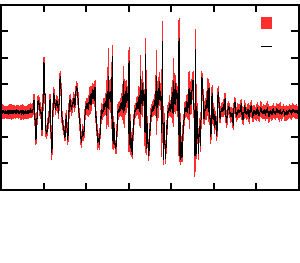
\includegraphics{voltage_0_108_gap_between_pulses_250_no_imaging_av_with_sd_means1_large}}%
    \gplfronttext
  \end{picture}%
\endgroup
}
 \quad
  \subfloat[2nd pulse - \unit{250}\micro\second]{
    \label{fig:exp:control:av:time:250:second}
    % GNUPLOT: LaTeX picture with Postscript
\begingroup
  \makeatletter
  \providecommand\color[2][]{%
    \GenericError{(gnuplot) \space\space\space\@spaces}{%
      Package color not loaded in conjunction with
      terminal option `colourtext'%
    }{See the gnuplot documentation for explanation.%
    }{Either use 'blacktext' in gnuplot or load the package
      color.sty in LaTeX.}%
    \renewcommand\color[2][]{}%
  }%
  \providecommand\includegraphics[2][]{%
    \GenericError{(gnuplot) \space\space\space\@spaces}{%
      Package graphicx or graphics not loaded%
    }{See the gnuplot documentation for explanation.%
    }{The gnuplot epslatex terminal needs graphicx.sty or graphics.sty.}%
    \renewcommand\includegraphics[2][]{}%
  }%
  \providecommand\rotatebox[2]{#2}%
  \@ifundefined{ifGPcolor}{%
    \newif\ifGPcolor
    \GPcolortrue
  }{}%
  \@ifundefined{ifGPblacktext}{%
    \newif\ifGPblacktext
    \GPblacktexttrue
  }{}%
  % define a \g@addto@macro without @ in the name:
  \let\gplgaddtomacro\g@addto@macro
  % define empty templates for all commands taking text:
  \gdef\gplbacktext{}%
  \gdef\gplfronttext{}%
  \makeatother
  \ifGPblacktext
    % no textcolor at all
    \def\colorrgb#1{}%
    \def\colorgray#1{}%
  \else
    % gray or color?
    \ifGPcolor
      \def\colorrgb#1{\color[rgb]{#1}}%
      \def\colorgray#1{\color[gray]{#1}}%
      \expandafter\def\csname LTw\endcsname{\color{white}}%
      \expandafter\def\csname LTb\endcsname{\color{black}}%
      \expandafter\def\csname LTa\endcsname{\color{black}}%
      \expandafter\def\csname LT0\endcsname{\color[rgb]{1,0,0}}%
      \expandafter\def\csname LT1\endcsname{\color[rgb]{0,1,0}}%
      \expandafter\def\csname LT2\endcsname{\color[rgb]{0,0,1}}%
      \expandafter\def\csname LT3\endcsname{\color[rgb]{1,0,1}}%
      \expandafter\def\csname LT4\endcsname{\color[rgb]{0,1,1}}%
      \expandafter\def\csname LT5\endcsname{\color[rgb]{1,1,0}}%
      \expandafter\def\csname LT6\endcsname{\color[rgb]{0,0,0}}%
      \expandafter\def\csname LT7\endcsname{\color[rgb]{1,0.3,0}}%
      \expandafter\def\csname LT8\endcsname{\color[rgb]{0.5,0.5,0.5}}%
    \else
      % gray
      \def\colorrgb#1{\color{black}}%
      \def\colorgray#1{\color[gray]{#1}}%
      \expandafter\def\csname LTw\endcsname{\color{white}}%
      \expandafter\def\csname LTb\endcsname{\color{black}}%
      \expandafter\def\csname LTa\endcsname{\color{black}}%
      \expandafter\def\csname LT0\endcsname{\color{black}}%
      \expandafter\def\csname LT1\endcsname{\color{black}}%
      \expandafter\def\csname LT2\endcsname{\color{black}}%
      \expandafter\def\csname LT3\endcsname{\color{black}}%
      \expandafter\def\csname LT4\endcsname{\color{black}}%
      \expandafter\def\csname LT5\endcsname{\color{black}}%
      \expandafter\def\csname LT6\endcsname{\color{black}}%
      \expandafter\def\csname LT7\endcsname{\color{black}}%
      \expandafter\def\csname LT8\endcsname{\color{black}}%
    \fi
  \fi
  \setlength{\unitlength}{0.0500bp}%
  \begin{picture}(2880.00,2520.00)%
    \gplgaddtomacro\gplbacktext{%
      \csname LTb\endcsname%
      \put(-119,704){\makebox(0,0)[r]{\strut{}}}%
      \put(-119,926){\makebox(0,0)[r]{\strut{}}}%
      \put(-119,1147){\makebox(0,0)[r]{\strut{}}}%
      \put(-119,1369){\makebox(0,0)[r]{\strut{}}}%
      \put(-119,1590){\makebox(0,0)[r]{\strut{}}}%
      \put(-119,1812){\makebox(0,0)[r]{\strut{}}}%
      \put(-119,2033){\makebox(0,0)[r]{\strut{}}}%
      \put(-119,2255){\makebox(0,0)[r]{\strut{}}}%
      \put(-119,2476){\makebox(0,0)[r]{\strut{}}}%
      \put(13,484){\makebox(0,0){\strut{} 0}}%
      \put(421,484){\makebox(0,0){\strut{} 5}}%
      \put(828,484){\makebox(0,0){\strut{} 10}}%
      \put(1236,484){\makebox(0,0){\strut{} 15}}%
      \put(1643,484){\makebox(0,0){\strut{} 20}}%
      \put(2051,484){\makebox(0,0){\strut{} 25}}%
      \put(2458,484){\makebox(0,0){\strut{} 30}}%
      \put(2866,484){\makebox(0,0){\strut{} 35}}%
      \put(1439,154){\makebox(0,0){\strut{}time ($\mu$ s)}}%
    }%
    \gplgaddtomacro\gplfronttext{%
      \csname LTb\endcsname%
      \put(2381,2303){\makebox(0,0)[r]{\strut{}1-$\sigma$}}%
      \csname LTb\endcsname%
      \put(2381,2083){\makebox(0,0)[r]{\strut{}av.}}%
    }%
    \gplbacktext
    \put(0,0){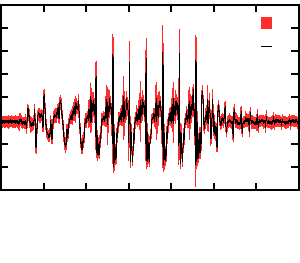
\includegraphics{voltage_0_108_gap_between_pulses_250_no_imaging_av_with_sd_means2_large}}%
    \gplfronttext
  \end{picture}%
\endgroup
}\\
\caption{
    The pressure received  by the imaging transducer when the driving wave is on but the imaging wave is off (receive-only).
    Each image is the average of 49 images, the first standard-deviation error bars are indicated.
    The time interval for each pair of images is indicated.
    The driving pressure is ... in all cases.
  }
\end{figure}
\begin{figure}[t]%
\ContinuedFloat
  \centering
  \subfloat[1st pulse - \unit{500}\micro\second]{
    \label{fig:exp:control:av:time:500:first}
    % GNUPLOT: LaTeX picture with Postscript
\begingroup
  \makeatletter
  \providecommand\color[2][]{%
    \GenericError{(gnuplot) \space\space\space\@spaces}{%
      Package color not loaded in conjunction with
      terminal option `colourtext'%
    }{See the gnuplot documentation for explanation.%
    }{Either use 'blacktext' in gnuplot or load the package
      color.sty in LaTeX.}%
    \renewcommand\color[2][]{}%
  }%
  \providecommand\includegraphics[2][]{%
    \GenericError{(gnuplot) \space\space\space\@spaces}{%
      Package graphicx or graphics not loaded%
    }{See the gnuplot documentation for explanation.%
    }{The gnuplot epslatex terminal needs graphicx.sty or graphics.sty.}%
    \renewcommand\includegraphics[2][]{}%
  }%
  \providecommand\rotatebox[2]{#2}%
  \@ifundefined{ifGPcolor}{%
    \newif\ifGPcolor
    \GPcolortrue
  }{}%
  \@ifundefined{ifGPblacktext}{%
    \newif\ifGPblacktext
    \GPblacktexttrue
  }{}%
  % define a \g@addto@macro without @ in the name:
  \let\gplgaddtomacro\g@addto@macro
  % define empty templates for all commands taking text:
  \gdef\gplbacktext{}%
  \gdef\gplfronttext{}%
  \makeatother
  \ifGPblacktext
    % no textcolor at all
    \def\colorrgb#1{}%
    \def\colorgray#1{}%
  \else
    % gray or color?
    \ifGPcolor
      \def\colorrgb#1{\color[rgb]{#1}}%
      \def\colorgray#1{\color[gray]{#1}}%
      \expandafter\def\csname LTw\endcsname{\color{white}}%
      \expandafter\def\csname LTb\endcsname{\color{black}}%
      \expandafter\def\csname LTa\endcsname{\color{black}}%
      \expandafter\def\csname LT0\endcsname{\color[rgb]{1,0,0}}%
      \expandafter\def\csname LT1\endcsname{\color[rgb]{0,1,0}}%
      \expandafter\def\csname LT2\endcsname{\color[rgb]{0,0,1}}%
      \expandafter\def\csname LT3\endcsname{\color[rgb]{1,0,1}}%
      \expandafter\def\csname LT4\endcsname{\color[rgb]{0,1,1}}%
      \expandafter\def\csname LT5\endcsname{\color[rgb]{1,1,0}}%
      \expandafter\def\csname LT6\endcsname{\color[rgb]{0,0,0}}%
      \expandafter\def\csname LT7\endcsname{\color[rgb]{1,0.3,0}}%
      \expandafter\def\csname LT8\endcsname{\color[rgb]{0.5,0.5,0.5}}%
    \else
      % gray
      \def\colorrgb#1{\color{black}}%
      \def\colorgray#1{\color[gray]{#1}}%
      \expandafter\def\csname LTw\endcsname{\color{white}}%
      \expandafter\def\csname LTb\endcsname{\color{black}}%
      \expandafter\def\csname LTa\endcsname{\color{black}}%
      \expandafter\def\csname LT0\endcsname{\color{black}}%
      \expandafter\def\csname LT1\endcsname{\color{black}}%
      \expandafter\def\csname LT2\endcsname{\color{black}}%
      \expandafter\def\csname LT3\endcsname{\color{black}}%
      \expandafter\def\csname LT4\endcsname{\color{black}}%
      \expandafter\def\csname LT5\endcsname{\color{black}}%
      \expandafter\def\csname LT6\endcsname{\color{black}}%
      \expandafter\def\csname LT7\endcsname{\color{black}}%
      \expandafter\def\csname LT8\endcsname{\color{black}}%
    \fi
  \fi
  \setlength{\unitlength}{0.0500bp}%
  \begin{picture}(2880.00,2520.00)%
    \gplgaddtomacro\gplbacktext{%
      \csname LTb\endcsname%
      \put(-119,704){\makebox(0,0)[r]{\strut{}-0.4}}%
      \put(-119,901){\makebox(0,0)[r]{\strut{}-0.3}}%
      \put(-119,1098){\makebox(0,0)[r]{\strut{}-0.2}}%
      \put(-119,1295){\makebox(0,0)[r]{\strut{}-0.1}}%
      \put(-119,1492){\makebox(0,0)[r]{\strut{} 0}}%
      \put(-119,1688){\makebox(0,0)[r]{\strut{} 0.1}}%
      \put(-119,1885){\makebox(0,0)[r]{\strut{} 0.2}}%
      \put(-119,2082){\makebox(0,0)[r]{\strut{} 0.3}}%
      \put(-119,2279){\makebox(0,0)[r]{\strut{} 0.4}}%
      \put(-119,2476){\makebox(0,0)[r]{\strut{} 0.5}}%
      \put(13,484){\makebox(0,0){\strut{} 0}}%
      \put(421,484){\makebox(0,0){\strut{} 5}}%
      \put(828,484){\makebox(0,0){\strut{} 10}}%
      \put(1236,484){\makebox(0,0){\strut{} 15}}%
      \put(1643,484){\makebox(0,0){\strut{} 20}}%
      \put(2051,484){\makebox(0,0){\strut{} 25}}%
      \put(2458,484){\makebox(0,0){\strut{} 30}}%
      \put(2866,484){\makebox(0,0){\strut{} 35}}%
      \put(-889,1590){\rotatebox{-270}{\makebox(0,0){\strut{}voltage (V)}}}%
      \put(1439,154){\makebox(0,0){\strut{}time ($\mu$ s)}}%
    }%
    \gplgaddtomacro\gplfronttext{%
      \csname LTb\endcsname%
      \put(2381,2303){\makebox(0,0)[r]{\strut{}1-$\sigma$}}%
      \csname LTb\endcsname%
      \put(2381,2083){\makebox(0,0)[r]{\strut{}av.}}%
    }%
    \gplbacktext
    \put(0,0){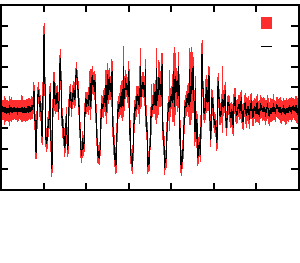
\includegraphics{voltage_0_108_gap_between_pulses_500_no_imaging_av_with_sd_means1_large}}%
    \gplfronttext
  \end{picture}%
\endgroup
}
 \quad
  \subfloat[2nd pulse - \unit{500}\micro\second]{
    \label{fig:exp:control:av:time:500:second}
    % GNUPLOT: LaTeX picture with Postscript
\begingroup
  \makeatletter
  \providecommand\color[2][]{%
    \GenericError{(gnuplot) \space\space\space\@spaces}{%
      Package color not loaded in conjunction with
      terminal option `colourtext'%
    }{See the gnuplot documentation for explanation.%
    }{Either use 'blacktext' in gnuplot or load the package
      color.sty in LaTeX.}%
    \renewcommand\color[2][]{}%
  }%
  \providecommand\includegraphics[2][]{%
    \GenericError{(gnuplot) \space\space\space\@spaces}{%
      Package graphicx or graphics not loaded%
    }{See the gnuplot documentation for explanation.%
    }{The gnuplot epslatex terminal needs graphicx.sty or graphics.sty.}%
    \renewcommand\includegraphics[2][]{}%
  }%
  \providecommand\rotatebox[2]{#2}%
  \@ifundefined{ifGPcolor}{%
    \newif\ifGPcolor
    \GPcolortrue
  }{}%
  \@ifundefined{ifGPblacktext}{%
    \newif\ifGPblacktext
    \GPblacktexttrue
  }{}%
  % define a \g@addto@macro without @ in the name:
  \let\gplgaddtomacro\g@addto@macro
  % define empty templates for all commands taking text:
  \gdef\gplbacktext{}%
  \gdef\gplfronttext{}%
  \makeatother
  \ifGPblacktext
    % no textcolor at all
    \def\colorrgb#1{}%
    \def\colorgray#1{}%
  \else
    % gray or color?
    \ifGPcolor
      \def\colorrgb#1{\color[rgb]{#1}}%
      \def\colorgray#1{\color[gray]{#1}}%
      \expandafter\def\csname LTw\endcsname{\color{white}}%
      \expandafter\def\csname LTb\endcsname{\color{black}}%
      \expandafter\def\csname LTa\endcsname{\color{black}}%
      \expandafter\def\csname LT0\endcsname{\color[rgb]{1,0,0}}%
      \expandafter\def\csname LT1\endcsname{\color[rgb]{0,1,0}}%
      \expandafter\def\csname LT2\endcsname{\color[rgb]{0,0,1}}%
      \expandafter\def\csname LT3\endcsname{\color[rgb]{1,0,1}}%
      \expandafter\def\csname LT4\endcsname{\color[rgb]{0,1,1}}%
      \expandafter\def\csname LT5\endcsname{\color[rgb]{1,1,0}}%
      \expandafter\def\csname LT6\endcsname{\color[rgb]{0,0,0}}%
      \expandafter\def\csname LT7\endcsname{\color[rgb]{1,0.3,0}}%
      \expandafter\def\csname LT8\endcsname{\color[rgb]{0.5,0.5,0.5}}%
    \else
      % gray
      \def\colorrgb#1{\color{black}}%
      \def\colorgray#1{\color[gray]{#1}}%
      \expandafter\def\csname LTw\endcsname{\color{white}}%
      \expandafter\def\csname LTb\endcsname{\color{black}}%
      \expandafter\def\csname LTa\endcsname{\color{black}}%
      \expandafter\def\csname LT0\endcsname{\color{black}}%
      \expandafter\def\csname LT1\endcsname{\color{black}}%
      \expandafter\def\csname LT2\endcsname{\color{black}}%
      \expandafter\def\csname LT3\endcsname{\color{black}}%
      \expandafter\def\csname LT4\endcsname{\color{black}}%
      \expandafter\def\csname LT5\endcsname{\color{black}}%
      \expandafter\def\csname LT6\endcsname{\color{black}}%
      \expandafter\def\csname LT7\endcsname{\color{black}}%
      \expandafter\def\csname LT8\endcsname{\color{black}}%
    \fi
  \fi
  \setlength{\unitlength}{0.0500bp}%
  \begin{picture}(2880.00,2520.00)%
    \gplgaddtomacro\gplbacktext{%
      \csname LTb\endcsname%
      \put(-119,704){\makebox(0,0)[r]{\strut{}}}%
      \put(-119,926){\makebox(0,0)[r]{\strut{}}}%
      \put(-119,1147){\makebox(0,0)[r]{\strut{}}}%
      \put(-119,1369){\makebox(0,0)[r]{\strut{}}}%
      \put(-119,1590){\makebox(0,0)[r]{\strut{}}}%
      \put(-119,1812){\makebox(0,0)[r]{\strut{}}}%
      \put(-119,2033){\makebox(0,0)[r]{\strut{}}}%
      \put(-119,2255){\makebox(0,0)[r]{\strut{}}}%
      \put(-119,2476){\makebox(0,0)[r]{\strut{}}}%
      \put(13,484){\makebox(0,0){\strut{} 0}}%
      \put(421,484){\makebox(0,0){\strut{} 5}}%
      \put(828,484){\makebox(0,0){\strut{} 10}}%
      \put(1236,484){\makebox(0,0){\strut{} 15}}%
      \put(1643,484){\makebox(0,0){\strut{} 20}}%
      \put(2051,484){\makebox(0,0){\strut{} 25}}%
      \put(2458,484){\makebox(0,0){\strut{} 30}}%
      \put(2866,484){\makebox(0,0){\strut{} 35}}%
      \put(1439,154){\makebox(0,0){\strut{}time ($\mu$ s)}}%
    }%
    \gplgaddtomacro\gplfronttext{%
      \csname LTb\endcsname%
      \put(2381,2303){\makebox(0,0)[r]{\strut{}1-$\sigma$}}%
      \csname LTb\endcsname%
      \put(2381,2083){\makebox(0,0)[r]{\strut{}av.}}%
    }%
    \gplbacktext
    \put(0,0){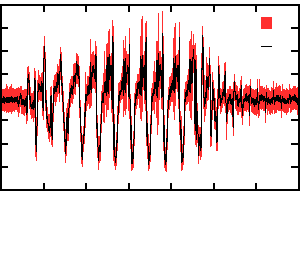
\includegraphics{voltage_0_108_gap_between_pulses_500_no_imaging_av_with_sd_means2_large}}%
    \gplfronttext
  \end{picture}%
\endgroup
}\\
 \subfloat[1st pulse - \unit{1000}\micro\second]{
    \label{fig:exp:control:av:time:1000:first}
    % GNUPLOT: LaTeX picture with Postscript
\begingroup
  \makeatletter
  \providecommand\color[2][]{%
    \GenericError{(gnuplot) \space\space\space\@spaces}{%
      Package color not loaded in conjunction with
      terminal option `colourtext'%
    }{See the gnuplot documentation for explanation.%
    }{Either use 'blacktext' in gnuplot or load the package
      color.sty in LaTeX.}%
    \renewcommand\color[2][]{}%
  }%
  \providecommand\includegraphics[2][]{%
    \GenericError{(gnuplot) \space\space\space\@spaces}{%
      Package graphicx or graphics not loaded%
    }{See the gnuplot documentation for explanation.%
    }{The gnuplot epslatex terminal needs graphicx.sty or graphics.sty.}%
    \renewcommand\includegraphics[2][]{}%
  }%
  \providecommand\rotatebox[2]{#2}%
  \@ifundefined{ifGPcolor}{%
    \newif\ifGPcolor
    \GPcolortrue
  }{}%
  \@ifundefined{ifGPblacktext}{%
    \newif\ifGPblacktext
    \GPblacktexttrue
  }{}%
  % define a \g@addto@macro without @ in the name:
  \let\gplgaddtomacro\g@addto@macro
  % define empty templates for all commands taking text:
  \gdef\gplbacktext{}%
  \gdef\gplfronttext{}%
  \makeatother
  \ifGPblacktext
    % no textcolor at all
    \def\colorrgb#1{}%
    \def\colorgray#1{}%
  \else
    % gray or color?
    \ifGPcolor
      \def\colorrgb#1{\color[rgb]{#1}}%
      \def\colorgray#1{\color[gray]{#1}}%
      \expandafter\def\csname LTw\endcsname{\color{white}}%
      \expandafter\def\csname LTb\endcsname{\color{black}}%
      \expandafter\def\csname LTa\endcsname{\color{black}}%
      \expandafter\def\csname LT0\endcsname{\color[rgb]{1,0,0}}%
      \expandafter\def\csname LT1\endcsname{\color[rgb]{0,1,0}}%
      \expandafter\def\csname LT2\endcsname{\color[rgb]{0,0,1}}%
      \expandafter\def\csname LT3\endcsname{\color[rgb]{1,0,1}}%
      \expandafter\def\csname LT4\endcsname{\color[rgb]{0,1,1}}%
      \expandafter\def\csname LT5\endcsname{\color[rgb]{1,1,0}}%
      \expandafter\def\csname LT6\endcsname{\color[rgb]{0,0,0}}%
      \expandafter\def\csname LT7\endcsname{\color[rgb]{1,0.3,0}}%
      \expandafter\def\csname LT8\endcsname{\color[rgb]{0.5,0.5,0.5}}%
    \else
      % gray
      \def\colorrgb#1{\color{black}}%
      \def\colorgray#1{\color[gray]{#1}}%
      \expandafter\def\csname LTw\endcsname{\color{white}}%
      \expandafter\def\csname LTb\endcsname{\color{black}}%
      \expandafter\def\csname LTa\endcsname{\color{black}}%
      \expandafter\def\csname LT0\endcsname{\color{black}}%
      \expandafter\def\csname LT1\endcsname{\color{black}}%
      \expandafter\def\csname LT2\endcsname{\color{black}}%
      \expandafter\def\csname LT3\endcsname{\color{black}}%
      \expandafter\def\csname LT4\endcsname{\color{black}}%
      \expandafter\def\csname LT5\endcsname{\color{black}}%
      \expandafter\def\csname LT6\endcsname{\color{black}}%
      \expandafter\def\csname LT7\endcsname{\color{black}}%
      \expandafter\def\csname LT8\endcsname{\color{black}}%
    \fi
  \fi
  \setlength{\unitlength}{0.0500bp}%
  \begin{picture}(2880.00,2520.00)%
    \gplgaddtomacro\gplbacktext{%
      \csname LTb\endcsname%
      \put(-119,704){\makebox(0,0)[r]{\strut{}-0.5}}%
      \put(-119,865){\makebox(0,0)[r]{\strut{}-0.4}}%
      \put(-119,1026){\makebox(0,0)[r]{\strut{}-0.3}}%
      \put(-119,1187){\makebox(0,0)[r]{\strut{}-0.2}}%
      \put(-119,1348){\makebox(0,0)[r]{\strut{}-0.1}}%
      \put(-119,1509){\makebox(0,0)[r]{\strut{} 0}}%
      \put(-119,1671){\makebox(0,0)[r]{\strut{} 0.1}}%
      \put(-119,1832){\makebox(0,0)[r]{\strut{} 0.2}}%
      \put(-119,1993){\makebox(0,0)[r]{\strut{} 0.3}}%
      \put(-119,2154){\makebox(0,0)[r]{\strut{} 0.4}}%
      \put(-119,2315){\makebox(0,0)[r]{\strut{} 0.5}}%
      \put(-119,2476){\makebox(0,0)[r]{\strut{} 0.6}}%
      \put(13,484){\makebox(0,0){\strut{} 0}}%
      \put(421,484){\makebox(0,0){\strut{} 5}}%
      \put(828,484){\makebox(0,0){\strut{} 10}}%
      \put(1236,484){\makebox(0,0){\strut{} 15}}%
      \put(1643,484){\makebox(0,0){\strut{} 20}}%
      \put(2051,484){\makebox(0,0){\strut{} 25}}%
      \put(2458,484){\makebox(0,0){\strut{} 30}}%
      \put(2866,484){\makebox(0,0){\strut{} 35}}%
      \put(-889,1590){\rotatebox{-270}{\makebox(0,0){\strut{}voltage (V)}}}%
      \put(1439,154){\makebox(0,0){\strut{}time ($\mu$ s)}}%
    }%
    \gplgaddtomacro\gplfronttext{%
      \csname LTb\endcsname%
      \put(2381,2303){\makebox(0,0)[r]{\strut{}1-$\sigma$}}%
      \csname LTb\endcsname%
      \put(2381,2083){\makebox(0,0)[r]{\strut{}av.}}%
    }%
    \gplbacktext
    \put(0,0){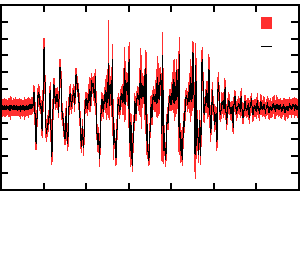
\includegraphics{voltage_0_108_gap_between_pulses_1000_no_imaging_av_with_sd_means1_large}}%
    \gplfronttext
  \end{picture}%
\endgroup
}
 \quad
  \subfloat[2nd pulse - \unit{1000}\micro\second]{
    \label{fig:exp:control:av:time:1000:second}
    % GNUPLOT: LaTeX picture with Postscript
\begingroup
  \makeatletter
  \providecommand\color[2][]{%
    \GenericError{(gnuplot) \space\space\space\@spaces}{%
      Package color not loaded in conjunction with
      terminal option `colourtext'%
    }{See the gnuplot documentation for explanation.%
    }{Either use 'blacktext' in gnuplot or load the package
      color.sty in LaTeX.}%
    \renewcommand\color[2][]{}%
  }%
  \providecommand\includegraphics[2][]{%
    \GenericError{(gnuplot) \space\space\space\@spaces}{%
      Package graphicx or graphics not loaded%
    }{See the gnuplot documentation for explanation.%
    }{The gnuplot epslatex terminal needs graphicx.sty or graphics.sty.}%
    \renewcommand\includegraphics[2][]{}%
  }%
  \providecommand\rotatebox[2]{#2}%
  \@ifundefined{ifGPcolor}{%
    \newif\ifGPcolor
    \GPcolortrue
  }{}%
  \@ifundefined{ifGPblacktext}{%
    \newif\ifGPblacktext
    \GPblacktexttrue
  }{}%
  % define a \g@addto@macro without @ in the name:
  \let\gplgaddtomacro\g@addto@macro
  % define empty templates for all commands taking text:
  \gdef\gplbacktext{}%
  \gdef\gplfronttext{}%
  \makeatother
  \ifGPblacktext
    % no textcolor at all
    \def\colorrgb#1{}%
    \def\colorgray#1{}%
  \else
    % gray or color?
    \ifGPcolor
      \def\colorrgb#1{\color[rgb]{#1}}%
      \def\colorgray#1{\color[gray]{#1}}%
      \expandafter\def\csname LTw\endcsname{\color{white}}%
      \expandafter\def\csname LTb\endcsname{\color{black}}%
      \expandafter\def\csname LTa\endcsname{\color{black}}%
      \expandafter\def\csname LT0\endcsname{\color[rgb]{1,0,0}}%
      \expandafter\def\csname LT1\endcsname{\color[rgb]{0,1,0}}%
      \expandafter\def\csname LT2\endcsname{\color[rgb]{0,0,1}}%
      \expandafter\def\csname LT3\endcsname{\color[rgb]{1,0,1}}%
      \expandafter\def\csname LT4\endcsname{\color[rgb]{0,1,1}}%
      \expandafter\def\csname LT5\endcsname{\color[rgb]{1,1,0}}%
      \expandafter\def\csname LT6\endcsname{\color[rgb]{0,0,0}}%
      \expandafter\def\csname LT7\endcsname{\color[rgb]{1,0.3,0}}%
      \expandafter\def\csname LT8\endcsname{\color[rgb]{0.5,0.5,0.5}}%
    \else
      % gray
      \def\colorrgb#1{\color{black}}%
      \def\colorgray#1{\color[gray]{#1}}%
      \expandafter\def\csname LTw\endcsname{\color{white}}%
      \expandafter\def\csname LTb\endcsname{\color{black}}%
      \expandafter\def\csname LTa\endcsname{\color{black}}%
      \expandafter\def\csname LT0\endcsname{\color{black}}%
      \expandafter\def\csname LT1\endcsname{\color{black}}%
      \expandafter\def\csname LT2\endcsname{\color{black}}%
      \expandafter\def\csname LT3\endcsname{\color{black}}%
      \expandafter\def\csname LT4\endcsname{\color{black}}%
      \expandafter\def\csname LT5\endcsname{\color{black}}%
      \expandafter\def\csname LT6\endcsname{\color{black}}%
      \expandafter\def\csname LT7\endcsname{\color{black}}%
      \expandafter\def\csname LT8\endcsname{\color{black}}%
    \fi
  \fi
  \setlength{\unitlength}{0.0500bp}%
  \begin{picture}(2880.00,2520.00)%
    \gplgaddtomacro\gplbacktext{%
      \csname LTb\endcsname%
      \put(-119,704){\makebox(0,0)[r]{\strut{}}}%
      \put(-119,865){\makebox(0,0)[r]{\strut{}}}%
      \put(-119,1026){\makebox(0,0)[r]{\strut{}}}%
      \put(-119,1187){\makebox(0,0)[r]{\strut{}}}%
      \put(-119,1348){\makebox(0,0)[r]{\strut{}}}%
      \put(-119,1509){\makebox(0,0)[r]{\strut{}}}%
      \put(-119,1671){\makebox(0,0)[r]{\strut{}}}%
      \put(-119,1832){\makebox(0,0)[r]{\strut{}}}%
      \put(-119,1993){\makebox(0,0)[r]{\strut{}}}%
      \put(-119,2154){\makebox(0,0)[r]{\strut{}}}%
      \put(-119,2315){\makebox(0,0)[r]{\strut{}}}%
      \put(-119,2476){\makebox(0,0)[r]{\strut{}}}%
      \put(13,484){\makebox(0,0){\strut{} 0}}%
      \put(421,484){\makebox(0,0){\strut{} 5}}%
      \put(828,484){\makebox(0,0){\strut{} 10}}%
      \put(1236,484){\makebox(0,0){\strut{} 15}}%
      \put(1643,484){\makebox(0,0){\strut{} 20}}%
      \put(2051,484){\makebox(0,0){\strut{} 25}}%
      \put(2458,484){\makebox(0,0){\strut{} 30}}%
      \put(2866,484){\makebox(0,0){\strut{} 35}}%
      \put(1439,154){\makebox(0,0){\strut{}time ($\mu$ s)}}%
    }%
    \gplgaddtomacro\gplfronttext{%
      \csname LTb\endcsname%
      \put(2381,2303){\makebox(0,0)[r]{\strut{}1-$\sigma$}}%
      \csname LTb\endcsname%
      \put(2381,2083){\makebox(0,0)[r]{\strut{}av.}}%
    }%
    \gplbacktext
    \put(0,0){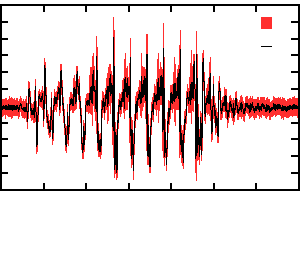
\includegraphics{voltage_0_108_gap_between_pulses_1000_no_imaging_av_with_sd_means2_large}}%
    \gplfronttext
  \end{picture}%
\endgroup
}\\
 \subfloat[1st pulse - \unit{5000}\micro\second]{
    \label{fig:exp:control:av:time:5000:first}
    % GNUPLOT: LaTeX picture with Postscript
\begingroup
  \makeatletter
  \providecommand\color[2][]{%
    \GenericError{(gnuplot) \space\space\space\@spaces}{%
      Package color not loaded in conjunction with
      terminal option `colourtext'%
    }{See the gnuplot documentation for explanation.%
    }{Either use 'blacktext' in gnuplot or load the package
      color.sty in LaTeX.}%
    \renewcommand\color[2][]{}%
  }%
  \providecommand\includegraphics[2][]{%
    \GenericError{(gnuplot) \space\space\space\@spaces}{%
      Package graphicx or graphics not loaded%
    }{See the gnuplot documentation for explanation.%
    }{The gnuplot epslatex terminal needs graphicx.sty or graphics.sty.}%
    \renewcommand\includegraphics[2][]{}%
  }%
  \providecommand\rotatebox[2]{#2}%
  \@ifundefined{ifGPcolor}{%
    \newif\ifGPcolor
    \GPcolortrue
  }{}%
  \@ifundefined{ifGPblacktext}{%
    \newif\ifGPblacktext
    \GPblacktexttrue
  }{}%
  % define a \g@addto@macro without @ in the name:
  \let\gplgaddtomacro\g@addto@macro
  % define empty templates for all commands taking text:
  \gdef\gplbacktext{}%
  \gdef\gplfronttext{}%
  \makeatother
  \ifGPblacktext
    % no textcolor at all
    \def\colorrgb#1{}%
    \def\colorgray#1{}%
  \else
    % gray or color?
    \ifGPcolor
      \def\colorrgb#1{\color[rgb]{#1}}%
      \def\colorgray#1{\color[gray]{#1}}%
      \expandafter\def\csname LTw\endcsname{\color{white}}%
      \expandafter\def\csname LTb\endcsname{\color{black}}%
      \expandafter\def\csname LTa\endcsname{\color{black}}%
      \expandafter\def\csname LT0\endcsname{\color[rgb]{1,0,0}}%
      \expandafter\def\csname LT1\endcsname{\color[rgb]{0,1,0}}%
      \expandafter\def\csname LT2\endcsname{\color[rgb]{0,0,1}}%
      \expandafter\def\csname LT3\endcsname{\color[rgb]{1,0,1}}%
      \expandafter\def\csname LT4\endcsname{\color[rgb]{0,1,1}}%
      \expandafter\def\csname LT5\endcsname{\color[rgb]{1,1,0}}%
      \expandafter\def\csname LT6\endcsname{\color[rgb]{0,0,0}}%
      \expandafter\def\csname LT7\endcsname{\color[rgb]{1,0.3,0}}%
      \expandafter\def\csname LT8\endcsname{\color[rgb]{0.5,0.5,0.5}}%
    \else
      % gray
      \def\colorrgb#1{\color{black}}%
      \def\colorgray#1{\color[gray]{#1}}%
      \expandafter\def\csname LTw\endcsname{\color{white}}%
      \expandafter\def\csname LTb\endcsname{\color{black}}%
      \expandafter\def\csname LTa\endcsname{\color{black}}%
      \expandafter\def\csname LT0\endcsname{\color{black}}%
      \expandafter\def\csname LT1\endcsname{\color{black}}%
      \expandafter\def\csname LT2\endcsname{\color{black}}%
      \expandafter\def\csname LT3\endcsname{\color{black}}%
      \expandafter\def\csname LT4\endcsname{\color{black}}%
      \expandafter\def\csname LT5\endcsname{\color{black}}%
      \expandafter\def\csname LT6\endcsname{\color{black}}%
      \expandafter\def\csname LT7\endcsname{\color{black}}%
      \expandafter\def\csname LT8\endcsname{\color{black}}%
    \fi
  \fi
  \setlength{\unitlength}{0.0500bp}%
  \begin{picture}(2880.00,2520.00)%
    \gplgaddtomacro\gplbacktext{%
      \csname LTb\endcsname%
      \put(-119,704){\makebox(0,0)[r]{\strut{}-0.6}}%
      \put(-119,999){\makebox(0,0)[r]{\strut{}-0.4}}%
      \put(-119,1295){\makebox(0,0)[r]{\strut{}-0.2}}%
      \put(-119,1590){\makebox(0,0)[r]{\strut{} 0}}%
      \put(-119,1885){\makebox(0,0)[r]{\strut{} 0.2}}%
      \put(-119,2181){\makebox(0,0)[r]{\strut{} 0.4}}%
      \put(-119,2476){\makebox(0,0)[r]{\strut{} 0.6}}%
      \put(13,484){\makebox(0,0){\strut{} 0}}%
      \put(421,484){\makebox(0,0){\strut{} 5}}%
      \put(828,484){\makebox(0,0){\strut{} 10}}%
      \put(1236,484){\makebox(0,0){\strut{} 15}}%
      \put(1643,484){\makebox(0,0){\strut{} 20}}%
      \put(2051,484){\makebox(0,0){\strut{} 25}}%
      \put(2458,484){\makebox(0,0){\strut{} 30}}%
      \put(2866,484){\makebox(0,0){\strut{} 35}}%
      \put(-889,1590){\rotatebox{-270}{\makebox(0,0){\strut{}voltage (V)}}}%
      \put(1439,154){\makebox(0,0){\strut{}time ($\mu$ s)}}%
    }%
    \gplgaddtomacro\gplfronttext{%
      \csname LTb\endcsname%
      \put(2381,2303){\makebox(0,0)[r]{\strut{}1-$\sigma$}}%
      \csname LTb\endcsname%
      \put(2381,2083){\makebox(0,0)[r]{\strut{}av.}}%
    }%
    \gplbacktext
    \put(0,0){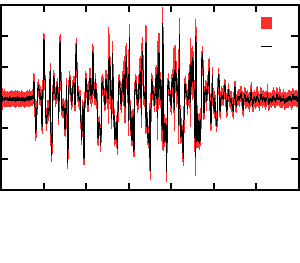
\includegraphics{voltage_0_108_gap_between_pulses_5000_no_imaging_av_with_sd_means1_large}}%
    \gplfronttext
  \end{picture}%
\endgroup
}
 \quad
  \subfloat[2nd pulse - \unit{5000}\micro\second]{
    \label{fig:exp:control:av:time:5000:second}
    % GNUPLOT: LaTeX picture with Postscript
\begingroup
  \makeatletter
  \providecommand\color[2][]{%
    \GenericError{(gnuplot) \space\space\space\@spaces}{%
      Package color not loaded in conjunction with
      terminal option `colourtext'%
    }{See the gnuplot documentation for explanation.%
    }{Either use 'blacktext' in gnuplot or load the package
      color.sty in LaTeX.}%
    \renewcommand\color[2][]{}%
  }%
  \providecommand\includegraphics[2][]{%
    \GenericError{(gnuplot) \space\space\space\@spaces}{%
      Package graphicx or graphics not loaded%
    }{See the gnuplot documentation for explanation.%
    }{The gnuplot epslatex terminal needs graphicx.sty or graphics.sty.}%
    \renewcommand\includegraphics[2][]{}%
  }%
  \providecommand\rotatebox[2]{#2}%
  \@ifundefined{ifGPcolor}{%
    \newif\ifGPcolor
    \GPcolortrue
  }{}%
  \@ifundefined{ifGPblacktext}{%
    \newif\ifGPblacktext
    \GPblacktexttrue
  }{}%
  % define a \g@addto@macro without @ in the name:
  \let\gplgaddtomacro\g@addto@macro
  % define empty templates for all commands taking text:
  \gdef\gplbacktext{}%
  \gdef\gplfronttext{}%
  \makeatother
  \ifGPblacktext
    % no textcolor at all
    \def\colorrgb#1{}%
    \def\colorgray#1{}%
  \else
    % gray or color?
    \ifGPcolor
      \def\colorrgb#1{\color[rgb]{#1}}%
      \def\colorgray#1{\color[gray]{#1}}%
      \expandafter\def\csname LTw\endcsname{\color{white}}%
      \expandafter\def\csname LTb\endcsname{\color{black}}%
      \expandafter\def\csname LTa\endcsname{\color{black}}%
      \expandafter\def\csname LT0\endcsname{\color[rgb]{1,0,0}}%
      \expandafter\def\csname LT1\endcsname{\color[rgb]{0,1,0}}%
      \expandafter\def\csname LT2\endcsname{\color[rgb]{0,0,1}}%
      \expandafter\def\csname LT3\endcsname{\color[rgb]{1,0,1}}%
      \expandafter\def\csname LT4\endcsname{\color[rgb]{0,1,1}}%
      \expandafter\def\csname LT5\endcsname{\color[rgb]{1,1,0}}%
      \expandafter\def\csname LT6\endcsname{\color[rgb]{0,0,0}}%
      \expandafter\def\csname LT7\endcsname{\color[rgb]{1,0.3,0}}%
      \expandafter\def\csname LT8\endcsname{\color[rgb]{0.5,0.5,0.5}}%
    \else
      % gray
      \def\colorrgb#1{\color{black}}%
      \def\colorgray#1{\color[gray]{#1}}%
      \expandafter\def\csname LTw\endcsname{\color{white}}%
      \expandafter\def\csname LTb\endcsname{\color{black}}%
      \expandafter\def\csname LTa\endcsname{\color{black}}%
      \expandafter\def\csname LT0\endcsname{\color{black}}%
      \expandafter\def\csname LT1\endcsname{\color{black}}%
      \expandafter\def\csname LT2\endcsname{\color{black}}%
      \expandafter\def\csname LT3\endcsname{\color{black}}%
      \expandafter\def\csname LT4\endcsname{\color{black}}%
      \expandafter\def\csname LT5\endcsname{\color{black}}%
      \expandafter\def\csname LT6\endcsname{\color{black}}%
      \expandafter\def\csname LT7\endcsname{\color{black}}%
      \expandafter\def\csname LT8\endcsname{\color{black}}%
    \fi
  \fi
  \setlength{\unitlength}{0.0500bp}%
  \begin{picture}(2880.00,2520.00)%
    \gplgaddtomacro\gplbacktext{%
      \csname LTb\endcsname%
      \put(-119,704){\makebox(0,0)[r]{\strut{}}}%
      \put(-119,926){\makebox(0,0)[r]{\strut{}}}%
      \put(-119,1147){\makebox(0,0)[r]{\strut{}}}%
      \put(-119,1369){\makebox(0,0)[r]{\strut{}}}%
      \put(-119,1590){\makebox(0,0)[r]{\strut{}}}%
      \put(-119,1812){\makebox(0,0)[r]{\strut{}}}%
      \put(-119,2033){\makebox(0,0)[r]{\strut{}}}%
      \put(-119,2255){\makebox(0,0)[r]{\strut{}}}%
      \put(-119,2476){\makebox(0,0)[r]{\strut{}}}%
      \put(13,484){\makebox(0,0){\strut{} 0}}%
      \put(421,484){\makebox(0,0){\strut{} 5}}%
      \put(828,484){\makebox(0,0){\strut{} 10}}%
      \put(1236,484){\makebox(0,0){\strut{} 15}}%
      \put(1643,484){\makebox(0,0){\strut{} 20}}%
      \put(2051,484){\makebox(0,0){\strut{} 25}}%
      \put(2458,484){\makebox(0,0){\strut{} 30}}%
      \put(2866,484){\makebox(0,0){\strut{} 35}}%
      \put(1439,154){\makebox(0,0){\strut{}time ($\mu$ s)}}%
    }%
    \gplgaddtomacro\gplfronttext{%
      \csname LTb\endcsname%
      \put(2381,2303){\makebox(0,0)[r]{\strut{}1-$\sigma$}}%
      \csname LTb\endcsname%
      \put(2381,2083){\makebox(0,0)[r]{\strut{}av.}}%
    }%
    \gplbacktext
    \put(0,0){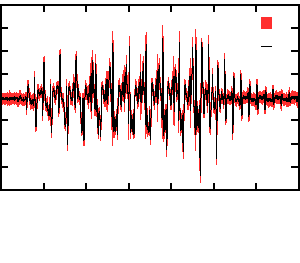
\includegraphics{voltage_0_108_gap_between_pulses_5000_no_imaging_av_with_sd_means2_large}}%
    \gplfronttext
  \end{picture}%
\endgroup
}\\
%subfloat[1st pulse - 12000]{
%   \label{fig:av:108:12000_ex:first}
%   % GNUPLOT: LaTeX picture with Postscript
\begingroup
  \makeatletter
  \providecommand\color[2][]{%
    \GenericError{(gnuplot) \space\space\space\@spaces}{%
      Package color not loaded in conjunction with
      terminal option `colourtext'%
    }{See the gnuplot documentation for explanation.%
    }{Either use 'blacktext' in gnuplot or load the package
      color.sty in LaTeX.}%
    \renewcommand\color[2][]{}%
  }%
  \providecommand\includegraphics[2][]{%
    \GenericError{(gnuplot) \space\space\space\@spaces}{%
      Package graphicx or graphics not loaded%
    }{See the gnuplot documentation for explanation.%
    }{The gnuplot epslatex terminal needs graphicx.sty or graphics.sty.}%
    \renewcommand\includegraphics[2][]{}%
  }%
  \providecommand\rotatebox[2]{#2}%
  \@ifundefined{ifGPcolor}{%
    \newif\ifGPcolor
    \GPcolortrue
  }{}%
  \@ifundefined{ifGPblacktext}{%
    \newif\ifGPblacktext
    \GPblacktexttrue
  }{}%
  % define a \g@addto@macro without @ in the name:
  \let\gplgaddtomacro\g@addto@macro
  % define empty templates for all commands taking text:
  \gdef\gplbacktext{}%
  \gdef\gplfronttext{}%
  \makeatother
  \ifGPblacktext
    % no textcolor at all
    \def\colorrgb#1{}%
    \def\colorgray#1{}%
  \else
    % gray or color?
    \ifGPcolor
      \def\colorrgb#1{\color[rgb]{#1}}%
      \def\colorgray#1{\color[gray]{#1}}%
      \expandafter\def\csname LTw\endcsname{\color{white}}%
      \expandafter\def\csname LTb\endcsname{\color{black}}%
      \expandafter\def\csname LTa\endcsname{\color{black}}%
      \expandafter\def\csname LT0\endcsname{\color[rgb]{1,0,0}}%
      \expandafter\def\csname LT1\endcsname{\color[rgb]{0,1,0}}%
      \expandafter\def\csname LT2\endcsname{\color[rgb]{0,0,1}}%
      \expandafter\def\csname LT3\endcsname{\color[rgb]{1,0,1}}%
      \expandafter\def\csname LT4\endcsname{\color[rgb]{0,1,1}}%
      \expandafter\def\csname LT5\endcsname{\color[rgb]{1,1,0}}%
      \expandafter\def\csname LT6\endcsname{\color[rgb]{0,0,0}}%
      \expandafter\def\csname LT7\endcsname{\color[rgb]{1,0.3,0}}%
      \expandafter\def\csname LT8\endcsname{\color[rgb]{0.5,0.5,0.5}}%
    \else
      % gray
      \def\colorrgb#1{\color{black}}%
      \def\colorgray#1{\color[gray]{#1}}%
      \expandafter\def\csname LTw\endcsname{\color{white}}%
      \expandafter\def\csname LTb\endcsname{\color{black}}%
      \expandafter\def\csname LTa\endcsname{\color{black}}%
      \expandafter\def\csname LT0\endcsname{\color{black}}%
      \expandafter\def\csname LT1\endcsname{\color{black}}%
      \expandafter\def\csname LT2\endcsname{\color{black}}%
      \expandafter\def\csname LT3\endcsname{\color{black}}%
      \expandafter\def\csname LT4\endcsname{\color{black}}%
      \expandafter\def\csname LT5\endcsname{\color{black}}%
      \expandafter\def\csname LT6\endcsname{\color{black}}%
      \expandafter\def\csname LT7\endcsname{\color{black}}%
      \expandafter\def\csname LT8\endcsname{\color{black}}%
    \fi
  \fi
  \setlength{\unitlength}{0.0500bp}%
  \begin{picture}(2880.00,2520.00)%
    \gplgaddtomacro\gplbacktext{%
      \csname LTb\endcsname%
      \put(-119,782){\makebox(0,0)[r]{\strut{}-1}}%
      \put(-119,1040){\makebox(0,0)[r]{\strut{}-0.5}}%
      \put(-119,1298){\makebox(0,0)[r]{\strut{} 0}}%
      \put(-119,1556){\makebox(0,0)[r]{\strut{} 0.5}}%
      \put(-119,1814){\makebox(0,0)[r]{\strut{} 1}}%
      \put(-119,2072){\makebox(0,0)[r]{\strut{} 1.5}}%
      \put(-119,2330){\makebox(0,0)[r]{\strut{} 2}}%
      \put(13,484){\makebox(0,0){\strut{} 0}}%
      \put(421,484){\makebox(0,0){\strut{} 5}}%
      \put(828,484){\makebox(0,0){\strut{} 10}}%
      \put(1236,484){\makebox(0,0){\strut{} 15}}%
      \put(1643,484){\makebox(0,0){\strut{} 20}}%
      \put(2051,484){\makebox(0,0){\strut{} 25}}%
      \put(2458,484){\makebox(0,0){\strut{} 30}}%
      \put(2866,484){\makebox(0,0){\strut{} 35}}%
      \put(-889,1590){\rotatebox{-270}{\makebox(0,0){\strut{}voltage (V)}}}%
      \put(1439,154){\makebox(0,0){\strut{}time ($\mu$ s)}}%
    }%
    \gplgaddtomacro\gplfronttext{%
      \csname LTb\endcsname%
      \put(2381,2303){\makebox(0,0)[r]{\strut{}1-$\sigma$}}%
      \csname LTb\endcsname%
      \put(2381,2083){\makebox(0,0)[r]{\strut{}av.}}%
    }%
    \gplbacktext
    \put(0,0){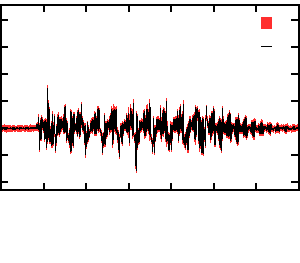
\includegraphics{voltage_0_108_gap_between_pulses_12000_no_imaging_av_with_sd_means1_large}}%
    \gplfronttext
  \end{picture}%
\endgroup
}
%\quad
% \subfloat[2nd pulse - 12000]{
%   \label{fig:av:108:12000_ex:second}
%   % GNUPLOT: LaTeX picture with Postscript
\begingroup
  \makeatletter
  \providecommand\color[2][]{%
    \GenericError{(gnuplot) \space\space\space\@spaces}{%
      Package color not loaded in conjunction with
      terminal option `colourtext'%
    }{See the gnuplot documentation for explanation.%
    }{Either use 'blacktext' in gnuplot or load the package
      color.sty in LaTeX.}%
    \renewcommand\color[2][]{}%
  }%
  \providecommand\includegraphics[2][]{%
    \GenericError{(gnuplot) \space\space\space\@spaces}{%
      Package graphicx or graphics not loaded%
    }{See the gnuplot documentation for explanation.%
    }{The gnuplot epslatex terminal needs graphicx.sty or graphics.sty.}%
    \renewcommand\includegraphics[2][]{}%
  }%
  \providecommand\rotatebox[2]{#2}%
  \@ifundefined{ifGPcolor}{%
    \newif\ifGPcolor
    \GPcolortrue
  }{}%
  \@ifundefined{ifGPblacktext}{%
    \newif\ifGPblacktext
    \GPblacktexttrue
  }{}%
  % define a \g@addto@macro without @ in the name:
  \let\gplgaddtomacro\g@addto@macro
  % define empty templates for all commands taking text:
  \gdef\gplbacktext{}%
  \gdef\gplfronttext{}%
  \makeatother
  \ifGPblacktext
    % no textcolor at all
    \def\colorrgb#1{}%
    \def\colorgray#1{}%
  \else
    % gray or color?
    \ifGPcolor
      \def\colorrgb#1{\color[rgb]{#1}}%
      \def\colorgray#1{\color[gray]{#1}}%
      \expandafter\def\csname LTw\endcsname{\color{white}}%
      \expandafter\def\csname LTb\endcsname{\color{black}}%
      \expandafter\def\csname LTa\endcsname{\color{black}}%
      \expandafter\def\csname LT0\endcsname{\color[rgb]{1,0,0}}%
      \expandafter\def\csname LT1\endcsname{\color[rgb]{0,1,0}}%
      \expandafter\def\csname LT2\endcsname{\color[rgb]{0,0,1}}%
      \expandafter\def\csname LT3\endcsname{\color[rgb]{1,0,1}}%
      \expandafter\def\csname LT4\endcsname{\color[rgb]{0,1,1}}%
      \expandafter\def\csname LT5\endcsname{\color[rgb]{1,1,0}}%
      \expandafter\def\csname LT6\endcsname{\color[rgb]{0,0,0}}%
      \expandafter\def\csname LT7\endcsname{\color[rgb]{1,0.3,0}}%
      \expandafter\def\csname LT8\endcsname{\color[rgb]{0.5,0.5,0.5}}%
    \else
      % gray
      \def\colorrgb#1{\color{black}}%
      \def\colorgray#1{\color[gray]{#1}}%
      \expandafter\def\csname LTw\endcsname{\color{white}}%
      \expandafter\def\csname LTb\endcsname{\color{black}}%
      \expandafter\def\csname LTa\endcsname{\color{black}}%
      \expandafter\def\csname LT0\endcsname{\color{black}}%
      \expandafter\def\csname LT1\endcsname{\color{black}}%
      \expandafter\def\csname LT2\endcsname{\color{black}}%
      \expandafter\def\csname LT3\endcsname{\color{black}}%
      \expandafter\def\csname LT4\endcsname{\color{black}}%
      \expandafter\def\csname LT5\endcsname{\color{black}}%
      \expandafter\def\csname LT6\endcsname{\color{black}}%
      \expandafter\def\csname LT7\endcsname{\color{black}}%
      \expandafter\def\csname LT8\endcsname{\color{black}}%
    \fi
  \fi
  \setlength{\unitlength}{0.0500bp}%
  \begin{picture}(2880.00,2520.00)%
    \gplgaddtomacro\gplbacktext{%
      \csname LTb\endcsname%
      \put(-119,782){\makebox(0,0)[r]{\strut{}}}%
      \put(-119,1040){\makebox(0,0)[r]{\strut{}}}%
      \put(-119,1298){\makebox(0,0)[r]{\strut{}}}%
      \put(-119,1556){\makebox(0,0)[r]{\strut{}}}%
      \put(-119,1814){\makebox(0,0)[r]{\strut{}}}%
      \put(-119,2072){\makebox(0,0)[r]{\strut{}}}%
      \put(-119,2330){\makebox(0,0)[r]{\strut{}}}%
      \put(13,484){\makebox(0,0){\strut{} 0}}%
      \put(421,484){\makebox(0,0){\strut{} 5}}%
      \put(828,484){\makebox(0,0){\strut{} 10}}%
      \put(1236,484){\makebox(0,0){\strut{} 15}}%
      \put(1643,484){\makebox(0,0){\strut{} 20}}%
      \put(2051,484){\makebox(0,0){\strut{} 25}}%
      \put(2458,484){\makebox(0,0){\strut{} 30}}%
      \put(2866,484){\makebox(0,0){\strut{} 35}}%
      \put(1439,154){\makebox(0,0){\strut{}time ($\mu$ s)}}%
    }%
    \gplgaddtomacro\gplfronttext{%
      \csname LTb\endcsname%
      \put(2381,2303){\makebox(0,0)[r]{\strut{}1-$\sigma$}}%
      \csname LTb\endcsname%
      \put(2381,2083){\makebox(0,0)[r]{\strut{}av.}}%
    }%
    \gplbacktext
    \put(0,0){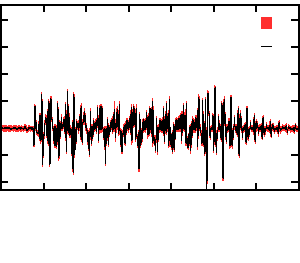
\includegraphics{voltage_0_108_gap_between_pulses_12000_no_imaging_av_with_sd_means2_large}}%
    \gplfronttext
  \end{picture}%
\endgroup
}
  \caption{
    (continued) The pressure received  by the imaging transducer when the driving wave is on but the imaging wave is off (receive-only).
    Each image is the average of 49 images, the first standard-deviation error bars are indicated.
    The time interval for each pair of images is indicated.
    The driving pressure is \pOEE\ in all cases.
  }
  \label{fig:exp:control:av:time}
\end{figure}

It is an opportunity because it gives a  means of sizing the generated bubbles.
Varying the interval between the pulses until they become stable
provides an upper bound on the lifetime (and therefore radius)
for the generated bubbles.

In \figref{exp:control:av:time} the interval between the pulses is examined 
for the pressure of \pOOE.
This pressure is chosen because it is one of the more moderate pressures 
for which \figref{exp:control:av:pressure:108:first}-\subref{fig:exp:control:av:pressure:108:second} 
demonstrates significant bubble interaction.

The forward scattering for when the time lag between driving pulses 
is between \unit{100}\micro\second\ and \unit{250}\micro\second\ (\figref{exp:control:av:time:100:first}-\subref{fig:exp:control:av:time:250:second}) are similar.
In all cases the interaction with the second pulse is stronger than the first,
but when each of the respective second pulses are compared no temporal effects are obvious.
The temporal durations of \unit{150}\micro\second\ and \unit{250}\micro\second\ look particularly similar.


For the larger durations of \figref{exp:control:av:time:500:first}-\subref{fig:exp:control:av:time:5000:second}
a much depleted interaction is found for both the first and second pulse.
While dissolution of a generated bubble would account for a reduced interaction in the second pulse,
the interaction with the first pulse should be the same in  all cases.
\Figref{exp:control:av:time:500:first}-\subref{fig:exp:control:av:time:5000:second}
is therefore most likely to result from a gradual change in the fundamental bubble population of the sample.

For each temporal offset three experiments are carried out.
First the control where the imaging transducer is in receive mode only.
Secondly when the imaging transducer coincides with the first driving pulse at the focus,
and then finally when the imaging transducer is timed to coincide with the second driving pulse.
Each of these experiments are repeated 50 times, meaning that the driving pulse
fires 300 times for every temporal offset.
It seems that the bubble population remains fairly constant over the first thousand or so driving pulses,
but looses bubbles by the time the longer pulsations are investigated.






\begin{figure}[t]%
  \centering
% \quad
%  \subfloat[2nd pulse - 100]{
%    \label{fig:exp:control:av:time:100:diff}
%    % GNUPLOT: LaTeX picture with Postscript
\begingroup
  \makeatletter
  \providecommand\color[2][]{%
    \GenericError{(gnuplot) \space\space\space\@spaces}{%
      Package color not loaded in conjunction with
      terminal option `colourtext'%
    }{See the gnuplot documentation for explanation.%
    }{Either use 'blacktext' in gnuplot or load the package
      color.sty in LaTeX.}%
    \renewcommand\color[2][]{}%
  }%
  \providecommand\includegraphics[2][]{%
    \GenericError{(gnuplot) \space\space\space\@spaces}{%
      Package graphicx or graphics not loaded%
    }{See the gnuplot documentation for explanation.%
    }{The gnuplot epslatex terminal needs graphicx.sty or graphics.sty.}%
    \renewcommand\includegraphics[2][]{}%
  }%
  \providecommand\rotatebox[2]{#2}%
  \@ifundefined{ifGPcolor}{%
    \newif\ifGPcolor
    \GPcolortrue
  }{}%
  \@ifundefined{ifGPblacktext}{%
    \newif\ifGPblacktext
    \GPblacktexttrue
  }{}%
  % define a \g@addto@macro without @ in the name:
  \let\gplgaddtomacro\g@addto@macro
  % define empty templates for all commands taking text:
  \gdef\gplbacktext{}%
  \gdef\gplfronttext{}%
  \makeatother
  \ifGPblacktext
    % no textcolor at all
    \def\colorrgb#1{}%
    \def\colorgray#1{}%
  \else
    % gray or color?
    \ifGPcolor
      \def\colorrgb#1{\color[rgb]{#1}}%
      \def\colorgray#1{\color[gray]{#1}}%
      \expandafter\def\csname LTw\endcsname{\color{white}}%
      \expandafter\def\csname LTb\endcsname{\color{black}}%
      \expandafter\def\csname LTa\endcsname{\color{black}}%
      \expandafter\def\csname LT0\endcsname{\color[rgb]{1,0,0}}%
      \expandafter\def\csname LT1\endcsname{\color[rgb]{0,1,0}}%
      \expandafter\def\csname LT2\endcsname{\color[rgb]{0,0,1}}%
      \expandafter\def\csname LT3\endcsname{\color[rgb]{1,0,1}}%
      \expandafter\def\csname LT4\endcsname{\color[rgb]{0,1,1}}%
      \expandafter\def\csname LT5\endcsname{\color[rgb]{1,1,0}}%
      \expandafter\def\csname LT6\endcsname{\color[rgb]{0,0,0}}%
      \expandafter\def\csname LT7\endcsname{\color[rgb]{1,0.3,0}}%
      \expandafter\def\csname LT8\endcsname{\color[rgb]{0.5,0.5,0.5}}%
    \else
      % gray
      \def\colorrgb#1{\color{black}}%
      \def\colorgray#1{\color[gray]{#1}}%
      \expandafter\def\csname LTw\endcsname{\color{white}}%
      \expandafter\def\csname LTb\endcsname{\color{black}}%
      \expandafter\def\csname LTa\endcsname{\color{black}}%
      \expandafter\def\csname LT0\endcsname{\color{black}}%
      \expandafter\def\csname LT1\endcsname{\color{black}}%
      \expandafter\def\csname LT2\endcsname{\color{black}}%
      \expandafter\def\csname LT3\endcsname{\color{black}}%
      \expandafter\def\csname LT4\endcsname{\color{black}}%
      \expandafter\def\csname LT5\endcsname{\color{black}}%
      \expandafter\def\csname LT6\endcsname{\color{black}}%
      \expandafter\def\csname LT7\endcsname{\color{black}}%
      \expandafter\def\csname LT8\endcsname{\color{black}}%
    \fi
  \fi
  \setlength{\unitlength}{0.0500bp}%
  \begin{picture}(2880.00,2520.00)%
    \gplgaddtomacro\gplbacktext{%
      \csname LTb\endcsname%
      \put(-119,704){\makebox(0,0)[r]{\strut{}-3}}%
      \put(-119,901){\makebox(0,0)[r]{\strut{}-2.5}}%
      \put(-119,1098){\makebox(0,0)[r]{\strut{}-2}}%
      \put(-119,1295){\makebox(0,0)[r]{\strut{}-1.5}}%
      \put(-119,1492){\makebox(0,0)[r]{\strut{}-1}}%
      \put(-119,1688){\makebox(0,0)[r]{\strut{}-0.5}}%
      \put(-119,1885){\makebox(0,0)[r]{\strut{} 0}}%
      \put(-119,2082){\makebox(0,0)[r]{\strut{} 0.5}}%
      \put(-119,2279){\makebox(0,0)[r]{\strut{} 1}}%
      \put(-119,2476){\makebox(0,0)[r]{\strut{} 1.5}}%
      \put(13,484){\makebox(0,0){\strut{} 0}}%
      \put(421,484){\makebox(0,0){\strut{} 5}}%
      \put(828,484){\makebox(0,0){\strut{} 10}}%
      \put(1236,484){\makebox(0,0){\strut{} 15}}%
      \put(1643,484){\makebox(0,0){\strut{} 20}}%
      \put(2051,484){\makebox(0,0){\strut{} 25}}%
      \put(2458,484){\makebox(0,0){\strut{} 30}}%
      \put(2866,484){\makebox(0,0){\strut{} 35}}%
      \put(-889,1590){\rotatebox{-270}{\makebox(0,0){\strut{}voltage (V)}}}%
      \put(1439,154){\makebox(0,0){\strut{}time ($\mu$ s)}}%
    }%
    \gplgaddtomacro\gplfronttext{%
      \csname LTb\endcsname%
      \put(2381,2303){\makebox(0,0)[r]{\strut{}1-$\sigma$}}%
      \csname LTb\endcsname%
      \put(2381,2083){\makebox(0,0)[r]{\strut{}av.}}%
    }%
    \gplbacktext
    \put(0,0){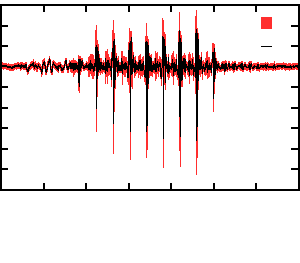
\includegraphics{voltage_0_108_gap_between_pulses_100_no_imaging_av_with_sd_meansSub_large}}%
    \gplfronttext
  \end{picture}%
\endgroup
}\\
 \quad
  \subfloat[\unit{150}\micro\second]{
    \label{fig:exp:control:av:time:150:diff}
    % GNUPLOT: LaTeX picture with Postscript
\begingroup
  \makeatletter
  \providecommand\color[2][]{%
    \GenericError{(gnuplot) \space\space\space\@spaces}{%
      Package color not loaded in conjunction with
      terminal option `colourtext'%
    }{See the gnuplot documentation for explanation.%
    }{Either use 'blacktext' in gnuplot or load the package
      color.sty in LaTeX.}%
    \renewcommand\color[2][]{}%
  }%
  \providecommand\includegraphics[2][]{%
    \GenericError{(gnuplot) \space\space\space\@spaces}{%
      Package graphicx or graphics not loaded%
    }{See the gnuplot documentation for explanation.%
    }{The gnuplot epslatex terminal needs graphicx.sty or graphics.sty.}%
    \renewcommand\includegraphics[2][]{}%
  }%
  \providecommand\rotatebox[2]{#2}%
  \@ifundefined{ifGPcolor}{%
    \newif\ifGPcolor
    \GPcolortrue
  }{}%
  \@ifundefined{ifGPblacktext}{%
    \newif\ifGPblacktext
    \GPblacktexttrue
  }{}%
  % define a \g@addto@macro without @ in the name:
  \let\gplgaddtomacro\g@addto@macro
  % define empty templates for all commands taking text:
  \gdef\gplbacktext{}%
  \gdef\gplfronttext{}%
  \makeatother
  \ifGPblacktext
    % no textcolor at all
    \def\colorrgb#1{}%
    \def\colorgray#1{}%
  \else
    % gray or color?
    \ifGPcolor
      \def\colorrgb#1{\color[rgb]{#1}}%
      \def\colorgray#1{\color[gray]{#1}}%
      \expandafter\def\csname LTw\endcsname{\color{white}}%
      \expandafter\def\csname LTb\endcsname{\color{black}}%
      \expandafter\def\csname LTa\endcsname{\color{black}}%
      \expandafter\def\csname LT0\endcsname{\color[rgb]{1,0,0}}%
      \expandafter\def\csname LT1\endcsname{\color[rgb]{0,1,0}}%
      \expandafter\def\csname LT2\endcsname{\color[rgb]{0,0,1}}%
      \expandafter\def\csname LT3\endcsname{\color[rgb]{1,0,1}}%
      \expandafter\def\csname LT4\endcsname{\color[rgb]{0,1,1}}%
      \expandafter\def\csname LT5\endcsname{\color[rgb]{1,1,0}}%
      \expandafter\def\csname LT6\endcsname{\color[rgb]{0,0,0}}%
      \expandafter\def\csname LT7\endcsname{\color[rgb]{1,0.3,0}}%
      \expandafter\def\csname LT8\endcsname{\color[rgb]{0.5,0.5,0.5}}%
    \else
      % gray
      \def\colorrgb#1{\color{black}}%
      \def\colorgray#1{\color[gray]{#1}}%
      \expandafter\def\csname LTw\endcsname{\color{white}}%
      \expandafter\def\csname LTb\endcsname{\color{black}}%
      \expandafter\def\csname LTa\endcsname{\color{black}}%
      \expandafter\def\csname LT0\endcsname{\color{black}}%
      \expandafter\def\csname LT1\endcsname{\color{black}}%
      \expandafter\def\csname LT2\endcsname{\color{black}}%
      \expandafter\def\csname LT3\endcsname{\color{black}}%
      \expandafter\def\csname LT4\endcsname{\color{black}}%
      \expandafter\def\csname LT5\endcsname{\color{black}}%
      \expandafter\def\csname LT6\endcsname{\color{black}}%
      \expandafter\def\csname LT7\endcsname{\color{black}}%
      \expandafter\def\csname LT8\endcsname{\color{black}}%
    \fi
  \fi
  \setlength{\unitlength}{0.0500bp}%
  \begin{picture}(2880.00,2520.00)%
    \gplgaddtomacro\gplbacktext{%
      \csname LTb\endcsname%
      \put(-119,704){\makebox(0,0)[r]{\strut{}-1.2}}%
      \put(-119,865){\makebox(0,0)[r]{\strut{}-1}}%
      \put(-119,1026){\makebox(0,0)[r]{\strut{}-0.8}}%
      \put(-119,1187){\makebox(0,0)[r]{\strut{}-0.6}}%
      \put(-119,1348){\makebox(0,0)[r]{\strut{}-0.4}}%
      \put(-119,1509){\makebox(0,0)[r]{\strut{}-0.2}}%
      \put(-119,1671){\makebox(0,0)[r]{\strut{} 0}}%
      \put(-119,1832){\makebox(0,0)[r]{\strut{} 0.2}}%
      \put(-119,1993){\makebox(0,0)[r]{\strut{} 0.4}}%
      \put(-119,2154){\makebox(0,0)[r]{\strut{} 0.6}}%
      \put(-119,2315){\makebox(0,0)[r]{\strut{} 0.8}}%
      \put(-119,2476){\makebox(0,0)[r]{\strut{} 1}}%
      \put(13,484){\makebox(0,0){\strut{} 0}}%
      \put(421,484){\makebox(0,0){\strut{} 5}}%
      \put(828,484){\makebox(0,0){\strut{} 10}}%
      \put(1236,484){\makebox(0,0){\strut{} 15}}%
      \put(1643,484){\makebox(0,0){\strut{} 20}}%
      \put(2051,484){\makebox(0,0){\strut{} 25}}%
      \put(2458,484){\makebox(0,0){\strut{} 30}}%
      \put(2866,484){\makebox(0,0){\strut{} 35}}%
      \put(-889,1590){\rotatebox{-270}{\makebox(0,0){\strut{}voltage (V)}}}%
      \put(1439,154){\makebox(0,0){\strut{}time ($\mu$ s)}}%
    }%
    \gplgaddtomacro\gplfronttext{%
      \csname LTb\endcsname%
      \put(2381,2303){\makebox(0,0)[r]{\strut{}1-$\sigma$}}%
      \csname LTb\endcsname%
      \put(2381,2083){\makebox(0,0)[r]{\strut{}av.}}%
    }%
    \gplbacktext
    \put(0,0){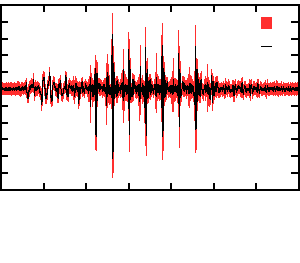
\includegraphics{voltage_0_108_gap_between_pulses_150_no_imaging_av_with_sd_meansSub_large}}%
    \gplfronttext
  \end{picture}%
\endgroup
}\\
 \quad
  \subfloat[\unit{250}\micro\second]{
    \label{fig:exp:control:av:time:250:diff}
    % GNUPLOT: LaTeX picture with Postscript
\begingroup
  \makeatletter
  \providecommand\color[2][]{%
    \GenericError{(gnuplot) \space\space\space\@spaces}{%
      Package color not loaded in conjunction with
      terminal option `colourtext'%
    }{See the gnuplot documentation for explanation.%
    }{Either use 'blacktext' in gnuplot or load the package
      color.sty in LaTeX.}%
    \renewcommand\color[2][]{}%
  }%
  \providecommand\includegraphics[2][]{%
    \GenericError{(gnuplot) \space\space\space\@spaces}{%
      Package graphicx or graphics not loaded%
    }{See the gnuplot documentation for explanation.%
    }{The gnuplot epslatex terminal needs graphicx.sty or graphics.sty.}%
    \renewcommand\includegraphics[2][]{}%
  }%
  \providecommand\rotatebox[2]{#2}%
  \@ifundefined{ifGPcolor}{%
    \newif\ifGPcolor
    \GPcolortrue
  }{}%
  \@ifundefined{ifGPblacktext}{%
    \newif\ifGPblacktext
    \GPblacktexttrue
  }{}%
  % define a \g@addto@macro without @ in the name:
  \let\gplgaddtomacro\g@addto@macro
  % define empty templates for all commands taking text:
  \gdef\gplbacktext{}%
  \gdef\gplfronttext{}%
  \makeatother
  \ifGPblacktext
    % no textcolor at all
    \def\colorrgb#1{}%
    \def\colorgray#1{}%
  \else
    % gray or color?
    \ifGPcolor
      \def\colorrgb#1{\color[rgb]{#1}}%
      \def\colorgray#1{\color[gray]{#1}}%
      \expandafter\def\csname LTw\endcsname{\color{white}}%
      \expandafter\def\csname LTb\endcsname{\color{black}}%
      \expandafter\def\csname LTa\endcsname{\color{black}}%
      \expandafter\def\csname LT0\endcsname{\color[rgb]{1,0,0}}%
      \expandafter\def\csname LT1\endcsname{\color[rgb]{0,1,0}}%
      \expandafter\def\csname LT2\endcsname{\color[rgb]{0,0,1}}%
      \expandafter\def\csname LT3\endcsname{\color[rgb]{1,0,1}}%
      \expandafter\def\csname LT4\endcsname{\color[rgb]{0,1,1}}%
      \expandafter\def\csname LT5\endcsname{\color[rgb]{1,1,0}}%
      \expandafter\def\csname LT6\endcsname{\color[rgb]{0,0,0}}%
      \expandafter\def\csname LT7\endcsname{\color[rgb]{1,0.3,0}}%
      \expandafter\def\csname LT8\endcsname{\color[rgb]{0.5,0.5,0.5}}%
    \else
      % gray
      \def\colorrgb#1{\color{black}}%
      \def\colorgray#1{\color[gray]{#1}}%
      \expandafter\def\csname LTw\endcsname{\color{white}}%
      \expandafter\def\csname LTb\endcsname{\color{black}}%
      \expandafter\def\csname LTa\endcsname{\color{black}}%
      \expandafter\def\csname LT0\endcsname{\color{black}}%
      \expandafter\def\csname LT1\endcsname{\color{black}}%
      \expandafter\def\csname LT2\endcsname{\color{black}}%
      \expandafter\def\csname LT3\endcsname{\color{black}}%
      \expandafter\def\csname LT4\endcsname{\color{black}}%
      \expandafter\def\csname LT5\endcsname{\color{black}}%
      \expandafter\def\csname LT6\endcsname{\color{black}}%
      \expandafter\def\csname LT7\endcsname{\color{black}}%
      \expandafter\def\csname LT8\endcsname{\color{black}}%
    \fi
  \fi
  \setlength{\unitlength}{0.0500bp}%
  \begin{picture}(2880.00,2520.00)%
    \gplgaddtomacro\gplbacktext{%
      \csname LTb\endcsname%
      \put(-119,704){\makebox(0,0)[r]{\strut{}-1}}%
      \put(-119,881){\makebox(0,0)[r]{\strut{}-0.8}}%
      \put(-119,1058){\makebox(0,0)[r]{\strut{}-0.6}}%
      \put(-119,1236){\makebox(0,0)[r]{\strut{}-0.4}}%
      \put(-119,1413){\makebox(0,0)[r]{\strut{}-0.2}}%
      \put(-119,1590){\makebox(0,0)[r]{\strut{} 0}}%
      \put(-119,1767){\makebox(0,0)[r]{\strut{} 0.2}}%
      \put(-119,1944){\makebox(0,0)[r]{\strut{} 0.4}}%
      \put(-119,2122){\makebox(0,0)[r]{\strut{} 0.6}}%
      \put(-119,2299){\makebox(0,0)[r]{\strut{} 0.8}}%
      \put(-119,2476){\makebox(0,0)[r]{\strut{} 1}}%
      \put(13,484){\makebox(0,0){\strut{} 0}}%
      \put(421,484){\makebox(0,0){\strut{} 5}}%
      \put(828,484){\makebox(0,0){\strut{} 10}}%
      \put(1236,484){\makebox(0,0){\strut{} 15}}%
      \put(1643,484){\makebox(0,0){\strut{} 20}}%
      \put(2051,484){\makebox(0,0){\strut{} 25}}%
      \put(2458,484){\makebox(0,0){\strut{} 30}}%
      \put(2866,484){\makebox(0,0){\strut{} 35}}%
      \put(-889,1590){\rotatebox{-270}{\makebox(0,0){\strut{}voltage (V)}}}%
      \put(1439,154){\makebox(0,0){\strut{}time ($\mu$ s)}}%
    }%
    \gplgaddtomacro\gplfronttext{%
      \csname LTb\endcsname%
      \put(2381,2303){\makebox(0,0)[r]{\strut{}1-$\sigma$}}%
      \csname LTb\endcsname%
      \put(2381,2083){\makebox(0,0)[r]{\strut{}av.}}%
    }%
    \gplbacktext
    \put(0,0){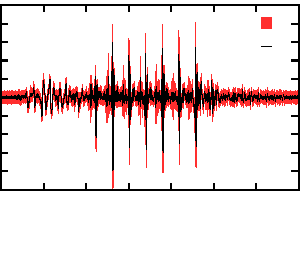
\includegraphics{voltage_0_108_gap_between_pulses_250_no_imaging_av_with_sd_meansSub_large}}%
    \gplfronttext
  \end{picture}%
\endgroup
}
\caption{
    The difference image for the pressure received  by the imaging transducer when the driving wave is on but the imaging wave is off (receive-only).
  }
  \label{fig:exp:control:av:time:diff}
\end{figure}


For the excess pressure to be evaluated the receive only scatter from the two pulses needs be the same.
The time lags of \unit{150}\micro\second\ and \unit{250}\micro\second\  between driving pulses 
look from \figref{exp:control:av:time}
to be the most promising in this regard.
The difference image 
- evaluated by subtracting the second received pulse image from the first -
is plotted in \figref{exp:control:av:time:diff}.


\begin{figure}[t]%
  \centering
%  \subfloat[1st pulse - 100]{
%    \label{fig:av:108:100_ex:first}
%    % GNUPLOT: LaTeX picture with Postscript
\begingroup
  \makeatletter
  \providecommand\color[2][]{%
    \GenericError{(gnuplot) \space\space\space\@spaces}{%
      Package color not loaded in conjunction with
      terminal option `colourtext'%
    }{See the gnuplot documentation for explanation.%
    }{Either use 'blacktext' in gnuplot or load the package
      color.sty in LaTeX.}%
    \renewcommand\color[2][]{}%
  }%
  \providecommand\includegraphics[2][]{%
    \GenericError{(gnuplot) \space\space\space\@spaces}{%
      Package graphicx or graphics not loaded%
    }{See the gnuplot documentation for explanation.%
    }{The gnuplot epslatex terminal needs graphicx.sty or graphics.sty.}%
    \renewcommand\includegraphics[2][]{}%
  }%
  \providecommand\rotatebox[2]{#2}%
  \@ifundefined{ifGPcolor}{%
    \newif\ifGPcolor
    \GPcolortrue
  }{}%
  \@ifundefined{ifGPblacktext}{%
    \newif\ifGPblacktext
    \GPblacktexttrue
  }{}%
  % define a \g@addto@macro without @ in the name:
  \let\gplgaddtomacro\g@addto@macro
  % define empty templates for all commands taking text:
  \gdef\gplbacktext{}%
  \gdef\gplfronttext{}%
  \makeatother
  \ifGPblacktext
    % no textcolor at all
    \def\colorrgb#1{}%
    \def\colorgray#1{}%
  \else
    % gray or color?
    \ifGPcolor
      \def\colorrgb#1{\color[rgb]{#1}}%
      \def\colorgray#1{\color[gray]{#1}}%
      \expandafter\def\csname LTw\endcsname{\color{white}}%
      \expandafter\def\csname LTb\endcsname{\color{black}}%
      \expandafter\def\csname LTa\endcsname{\color{black}}%
      \expandafter\def\csname LT0\endcsname{\color[rgb]{1,0,0}}%
      \expandafter\def\csname LT1\endcsname{\color[rgb]{0,1,0}}%
      \expandafter\def\csname LT2\endcsname{\color[rgb]{0,0,1}}%
      \expandafter\def\csname LT3\endcsname{\color[rgb]{1,0,1}}%
      \expandafter\def\csname LT4\endcsname{\color[rgb]{0,1,1}}%
      \expandafter\def\csname LT5\endcsname{\color[rgb]{1,1,0}}%
      \expandafter\def\csname LT6\endcsname{\color[rgb]{0,0,0}}%
      \expandafter\def\csname LT7\endcsname{\color[rgb]{1,0.3,0}}%
      \expandafter\def\csname LT8\endcsname{\color[rgb]{0.5,0.5,0.5}}%
    \else
      % gray
      \def\colorrgb#1{\color{black}}%
      \def\colorgray#1{\color[gray]{#1}}%
      \expandafter\def\csname LTw\endcsname{\color{white}}%
      \expandafter\def\csname LTb\endcsname{\color{black}}%
      \expandafter\def\csname LTa\endcsname{\color{black}}%
      \expandafter\def\csname LT0\endcsname{\color{black}}%
      \expandafter\def\csname LT1\endcsname{\color{black}}%
      \expandafter\def\csname LT2\endcsname{\color{black}}%
      \expandafter\def\csname LT3\endcsname{\color{black}}%
      \expandafter\def\csname LT4\endcsname{\color{black}}%
      \expandafter\def\csname LT5\endcsname{\color{black}}%
      \expandafter\def\csname LT6\endcsname{\color{black}}%
      \expandafter\def\csname LT7\endcsname{\color{black}}%
      \expandafter\def\csname LT8\endcsname{\color{black}}%
    \fi
  \fi
  \setlength{\unitlength}{0.0500bp}%
  \begin{picture}(2880.00,2520.00)%
    \gplgaddtomacro\gplbacktext{%
      \csname LTb\endcsname%
      \put(-119,704){\makebox(0,0)[r]{\strut{}-0.6}}%
      \put(-119,957){\makebox(0,0)[r]{\strut{}-0.4}}%
      \put(-119,1210){\makebox(0,0)[r]{\strut{}-0.2}}%
      \put(-119,1463){\makebox(0,0)[r]{\strut{} 0}}%
      \put(-119,1717){\makebox(0,0)[r]{\strut{} 0.2}}%
      \put(-119,1970){\makebox(0,0)[r]{\strut{} 0.4}}%
      \put(-119,2223){\makebox(0,0)[r]{\strut{} 0.6}}%
      \put(-119,2476){\makebox(0,0)[r]{\strut{} 0.8}}%
      \put(13,484){\makebox(0,0){\strut{} 17.5}}%
      \put(584,484){\makebox(0,0){\strut{} 18}}%
      \put(1154,484){\makebox(0,0){\strut{} 18.5}}%
      \put(1725,484){\makebox(0,0){\strut{} 19}}%
      \put(2295,484){\makebox(0,0){\strut{} 19.5}}%
      \put(2866,484){\makebox(0,0){\strut{} 20}}%
      \put(-889,1590){\rotatebox{-270}{\makebox(0,0){\strut{}voltage (V)}}}%
      \put(1439,154){\makebox(0,0){\strut{}time ($\mu$ s)}}%
    }%
    \gplgaddtomacro\gplfronttext{%
      \csname LTb\endcsname%
      \put(2381,2303){\makebox(0,0)[r]{\strut{}1-$\sigma$}}%
      \csname LTb\endcsname%
      \put(2381,2083){\makebox(0,0)[r]{\strut{}av.}}%
    }%
    \gplbacktext
    \put(0,0){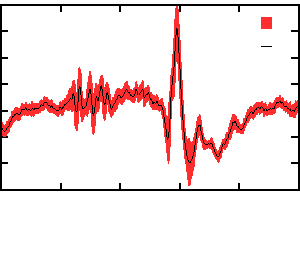
\includegraphics{voltage_0_108_gap_between_pulses_100_no_imaging_av_with_sd_means1_large2}}%
    \gplfronttext
  \end{picture}%
\endgroup
}
% \quad
%  \subfloat[2nd pulse - 100]{
%    \label{fig:av:108:100_ex:second}
%    % GNUPLOT: LaTeX picture with Postscript
\begingroup
  \makeatletter
  \providecommand\color[2][]{%
    \GenericError{(gnuplot) \space\space\space\@spaces}{%
      Package color not loaded in conjunction with
      terminal option `colourtext'%
    }{See the gnuplot documentation for explanation.%
    }{Either use 'blacktext' in gnuplot or load the package
      color.sty in LaTeX.}%
    \renewcommand\color[2][]{}%
  }%
  \providecommand\includegraphics[2][]{%
    \GenericError{(gnuplot) \space\space\space\@spaces}{%
      Package graphicx or graphics not loaded%
    }{See the gnuplot documentation for explanation.%
    }{The gnuplot epslatex terminal needs graphicx.sty or graphics.sty.}%
    \renewcommand\includegraphics[2][]{}%
  }%
  \providecommand\rotatebox[2]{#2}%
  \@ifundefined{ifGPcolor}{%
    \newif\ifGPcolor
    \GPcolortrue
  }{}%
  \@ifundefined{ifGPblacktext}{%
    \newif\ifGPblacktext
    \GPblacktexttrue
  }{}%
  % define a \g@addto@macro without @ in the name:
  \let\gplgaddtomacro\g@addto@macro
  % define empty templates for all commands taking text:
  \gdef\gplbacktext{}%
  \gdef\gplfronttext{}%
  \makeatother
  \ifGPblacktext
    % no textcolor at all
    \def\colorrgb#1{}%
    \def\colorgray#1{}%
  \else
    % gray or color?
    \ifGPcolor
      \def\colorrgb#1{\color[rgb]{#1}}%
      \def\colorgray#1{\color[gray]{#1}}%
      \expandafter\def\csname LTw\endcsname{\color{white}}%
      \expandafter\def\csname LTb\endcsname{\color{black}}%
      \expandafter\def\csname LTa\endcsname{\color{black}}%
      \expandafter\def\csname LT0\endcsname{\color[rgb]{1,0,0}}%
      \expandafter\def\csname LT1\endcsname{\color[rgb]{0,1,0}}%
      \expandafter\def\csname LT2\endcsname{\color[rgb]{0,0,1}}%
      \expandafter\def\csname LT3\endcsname{\color[rgb]{1,0,1}}%
      \expandafter\def\csname LT4\endcsname{\color[rgb]{0,1,1}}%
      \expandafter\def\csname LT5\endcsname{\color[rgb]{1,1,0}}%
      \expandafter\def\csname LT6\endcsname{\color[rgb]{0,0,0}}%
      \expandafter\def\csname LT7\endcsname{\color[rgb]{1,0.3,0}}%
      \expandafter\def\csname LT8\endcsname{\color[rgb]{0.5,0.5,0.5}}%
    \else
      % gray
      \def\colorrgb#1{\color{black}}%
      \def\colorgray#1{\color[gray]{#1}}%
      \expandafter\def\csname LTw\endcsname{\color{white}}%
      \expandafter\def\csname LTb\endcsname{\color{black}}%
      \expandafter\def\csname LTa\endcsname{\color{black}}%
      \expandafter\def\csname LT0\endcsname{\color{black}}%
      \expandafter\def\csname LT1\endcsname{\color{black}}%
      \expandafter\def\csname LT2\endcsname{\color{black}}%
      \expandafter\def\csname LT3\endcsname{\color{black}}%
      \expandafter\def\csname LT4\endcsname{\color{black}}%
      \expandafter\def\csname LT5\endcsname{\color{black}}%
      \expandafter\def\csname LT6\endcsname{\color{black}}%
      \expandafter\def\csname LT7\endcsname{\color{black}}%
      \expandafter\def\csname LT8\endcsname{\color{black}}%
    \fi
  \fi
  \setlength{\unitlength}{0.0500bp}%
  \begin{picture}(2880.00,2520.00)%
    \gplgaddtomacro\gplbacktext{%
      \csname LTb\endcsname%
      \put(-119,704){\makebox(0,0)[r]{\strut{}}}%
      \put(-119,926){\makebox(0,0)[r]{\strut{}}}%
      \put(-119,1147){\makebox(0,0)[r]{\strut{}}}%
      \put(-119,1369){\makebox(0,0)[r]{\strut{}}}%
      \put(-119,1590){\makebox(0,0)[r]{\strut{}}}%
      \put(-119,1812){\makebox(0,0)[r]{\strut{}}}%
      \put(-119,2033){\makebox(0,0)[r]{\strut{}}}%
      \put(-119,2255){\makebox(0,0)[r]{\strut{}}}%
      \put(-119,2476){\makebox(0,0)[r]{\strut{}}}%
      \put(13,484){\makebox(0,0){\strut{} 17.5}}%
      \put(584,484){\makebox(0,0){\strut{} 18}}%
      \put(1154,484){\makebox(0,0){\strut{} 18.5}}%
      \put(1725,484){\makebox(0,0){\strut{} 19}}%
      \put(2295,484){\makebox(0,0){\strut{} 19.5}}%
      \put(2866,484){\makebox(0,0){\strut{} 20}}%
      \put(1439,154){\makebox(0,0){\strut{}time ($\mu$ s)}}%
    }%
    \gplgaddtomacro\gplfronttext{%
      \csname LTb\endcsname%
      \put(2381,2303){\makebox(0,0)[r]{\strut{}1-$\sigma$}}%
      \csname LTb\endcsname%
      \put(2381,2083){\makebox(0,0)[r]{\strut{}av.}}%
    }%
    \gplbacktext
    \put(0,0){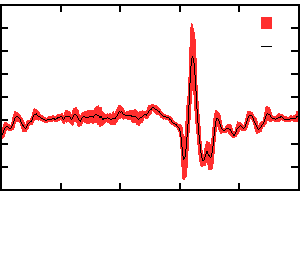
\includegraphics{voltage_0_108_gap_between_pulses_100_no_imaging_av_with_sd_means2_large2}}%
    \gplfronttext
  \end{picture}%
\endgroup
}\\
  \subfloat[1st pulse - \unit{150}\micro\second]{
    \label{fig:exp:control:av:time:150:detail:first}
    % GNUPLOT: LaTeX picture with Postscript
\begingroup
  \makeatletter
  \providecommand\color[2][]{%
    \GenericError{(gnuplot) \space\space\space\@spaces}{%
      Package color not loaded in conjunction with
      terminal option `colourtext'%
    }{See the gnuplot documentation for explanation.%
    }{Either use 'blacktext' in gnuplot or load the package
      color.sty in LaTeX.}%
    \renewcommand\color[2][]{}%
  }%
  \providecommand\includegraphics[2][]{%
    \GenericError{(gnuplot) \space\space\space\@spaces}{%
      Package graphicx or graphics not loaded%
    }{See the gnuplot documentation for explanation.%
    }{The gnuplot epslatex terminal needs graphicx.sty or graphics.sty.}%
    \renewcommand\includegraphics[2][]{}%
  }%
  \providecommand\rotatebox[2]{#2}%
  \@ifundefined{ifGPcolor}{%
    \newif\ifGPcolor
    \GPcolortrue
  }{}%
  \@ifundefined{ifGPblacktext}{%
    \newif\ifGPblacktext
    \GPblacktexttrue
  }{}%
  % define a \g@addto@macro without @ in the name:
  \let\gplgaddtomacro\g@addto@macro
  % define empty templates for all commands taking text:
  \gdef\gplbacktext{}%
  \gdef\gplfronttext{}%
  \makeatother
  \ifGPblacktext
    % no textcolor at all
    \def\colorrgb#1{}%
    \def\colorgray#1{}%
  \else
    % gray or color?
    \ifGPcolor
      \def\colorrgb#1{\color[rgb]{#1}}%
      \def\colorgray#1{\color[gray]{#1}}%
      \expandafter\def\csname LTw\endcsname{\color{white}}%
      \expandafter\def\csname LTb\endcsname{\color{black}}%
      \expandafter\def\csname LTa\endcsname{\color{black}}%
      \expandafter\def\csname LT0\endcsname{\color[rgb]{1,0,0}}%
      \expandafter\def\csname LT1\endcsname{\color[rgb]{0,1,0}}%
      \expandafter\def\csname LT2\endcsname{\color[rgb]{0,0,1}}%
      \expandafter\def\csname LT3\endcsname{\color[rgb]{1,0,1}}%
      \expandafter\def\csname LT4\endcsname{\color[rgb]{0,1,1}}%
      \expandafter\def\csname LT5\endcsname{\color[rgb]{1,1,0}}%
      \expandafter\def\csname LT6\endcsname{\color[rgb]{0,0,0}}%
      \expandafter\def\csname LT7\endcsname{\color[rgb]{1,0.3,0}}%
      \expandafter\def\csname LT8\endcsname{\color[rgb]{0.5,0.5,0.5}}%
    \else
      % gray
      \def\colorrgb#1{\color{black}}%
      \def\colorgray#1{\color[gray]{#1}}%
      \expandafter\def\csname LTw\endcsname{\color{white}}%
      \expandafter\def\csname LTb\endcsname{\color{black}}%
      \expandafter\def\csname LTa\endcsname{\color{black}}%
      \expandafter\def\csname LT0\endcsname{\color{black}}%
      \expandafter\def\csname LT1\endcsname{\color{black}}%
      \expandafter\def\csname LT2\endcsname{\color{black}}%
      \expandafter\def\csname LT3\endcsname{\color{black}}%
      \expandafter\def\csname LT4\endcsname{\color{black}}%
      \expandafter\def\csname LT5\endcsname{\color{black}}%
      \expandafter\def\csname LT6\endcsname{\color{black}}%
      \expandafter\def\csname LT7\endcsname{\color{black}}%
      \expandafter\def\csname LT8\endcsname{\color{black}}%
    \fi
  \fi
  \setlength{\unitlength}{0.0500bp}%
  \begin{picture}(2880.00,2520.00)%
    \gplgaddtomacro\gplbacktext{%
      \csname LTb\endcsname%
      \put(-119,704){\makebox(0,0)[r]{\strut{}-0.6}}%
      \put(-119,957){\makebox(0,0)[r]{\strut{}-0.4}}%
      \put(-119,1210){\makebox(0,0)[r]{\strut{}-0.2}}%
      \put(-119,1463){\makebox(0,0)[r]{\strut{} 0}}%
      \put(-119,1717){\makebox(0,0)[r]{\strut{} 0.2}}%
      \put(-119,1970){\makebox(0,0)[r]{\strut{} 0.4}}%
      \put(-119,2223){\makebox(0,0)[r]{\strut{} 0.6}}%
      \put(-119,2476){\makebox(0,0)[r]{\strut{} 0.8}}%
      \put(13,484){\makebox(0,0){\strut{} 17.5}}%
      \put(584,484){\makebox(0,0){\strut{} 18}}%
      \put(1154,484){\makebox(0,0){\strut{} 18.5}}%
      \put(1725,484){\makebox(0,0){\strut{} 19}}%
      \put(2295,484){\makebox(0,0){\strut{} 19.5}}%
      \put(2866,484){\makebox(0,0){\strut{} 20}}%
      \put(-889,1590){\rotatebox{-270}{\makebox(0,0){\strut{}voltage (V)}}}%
      \put(1439,154){\makebox(0,0){\strut{}time ($\mu$ s)}}%
    }%
    \gplgaddtomacro\gplfronttext{%
      \csname LTb\endcsname%
      \put(2381,2303){\makebox(0,0)[r]{\strut{}1-$\sigma$}}%
      \csname LTb\endcsname%
      \put(2381,2083){\makebox(0,0)[r]{\strut{}av.}}%
    }%
    \gplbacktext
    \put(0,0){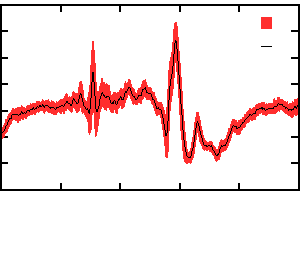
\includegraphics{voltage_0_108_gap_between_pulses_150_no_imaging_av_with_sd_means1_large2}}%
    \gplfronttext
  \end{picture}%
\endgroup
}
 \quad
  \subfloat[2nd pulse - \unit{150}\micro\second]{
    \label{fig:exp:control:av:time:150:detail:second}
    % GNUPLOT: LaTeX picture with Postscript
\begingroup
  \makeatletter
  \providecommand\color[2][]{%
    \GenericError{(gnuplot) \space\space\space\@spaces}{%
      Package color not loaded in conjunction with
      terminal option `colourtext'%
    }{See the gnuplot documentation for explanation.%
    }{Either use 'blacktext' in gnuplot or load the package
      color.sty in LaTeX.}%
    \renewcommand\color[2][]{}%
  }%
  \providecommand\includegraphics[2][]{%
    \GenericError{(gnuplot) \space\space\space\@spaces}{%
      Package graphicx or graphics not loaded%
    }{See the gnuplot documentation for explanation.%
    }{The gnuplot epslatex terminal needs graphicx.sty or graphics.sty.}%
    \renewcommand\includegraphics[2][]{}%
  }%
  \providecommand\rotatebox[2]{#2}%
  \@ifundefined{ifGPcolor}{%
    \newif\ifGPcolor
    \GPcolortrue
  }{}%
  \@ifundefined{ifGPblacktext}{%
    \newif\ifGPblacktext
    \GPblacktexttrue
  }{}%
  % define a \g@addto@macro without @ in the name:
  \let\gplgaddtomacro\g@addto@macro
  % define empty templates for all commands taking text:
  \gdef\gplbacktext{}%
  \gdef\gplfronttext{}%
  \makeatother
  \ifGPblacktext
    % no textcolor at all
    \def\colorrgb#1{}%
    \def\colorgray#1{}%
  \else
    % gray or color?
    \ifGPcolor
      \def\colorrgb#1{\color[rgb]{#1}}%
      \def\colorgray#1{\color[gray]{#1}}%
      \expandafter\def\csname LTw\endcsname{\color{white}}%
      \expandafter\def\csname LTb\endcsname{\color{black}}%
      \expandafter\def\csname LTa\endcsname{\color{black}}%
      \expandafter\def\csname LT0\endcsname{\color[rgb]{1,0,0}}%
      \expandafter\def\csname LT1\endcsname{\color[rgb]{0,1,0}}%
      \expandafter\def\csname LT2\endcsname{\color[rgb]{0,0,1}}%
      \expandafter\def\csname LT3\endcsname{\color[rgb]{1,0,1}}%
      \expandafter\def\csname LT4\endcsname{\color[rgb]{0,1,1}}%
      \expandafter\def\csname LT5\endcsname{\color[rgb]{1,1,0}}%
      \expandafter\def\csname LT6\endcsname{\color[rgb]{0,0,0}}%
      \expandafter\def\csname LT7\endcsname{\color[rgb]{1,0.3,0}}%
      \expandafter\def\csname LT8\endcsname{\color[rgb]{0.5,0.5,0.5}}%
    \else
      % gray
      \def\colorrgb#1{\color{black}}%
      \def\colorgray#1{\color[gray]{#1}}%
      \expandafter\def\csname LTw\endcsname{\color{white}}%
      \expandafter\def\csname LTb\endcsname{\color{black}}%
      \expandafter\def\csname LTa\endcsname{\color{black}}%
      \expandafter\def\csname LT0\endcsname{\color{black}}%
      \expandafter\def\csname LT1\endcsname{\color{black}}%
      \expandafter\def\csname LT2\endcsname{\color{black}}%
      \expandafter\def\csname LT3\endcsname{\color{black}}%
      \expandafter\def\csname LT4\endcsname{\color{black}}%
      \expandafter\def\csname LT5\endcsname{\color{black}}%
      \expandafter\def\csname LT6\endcsname{\color{black}}%
      \expandafter\def\csname LT7\endcsname{\color{black}}%
      \expandafter\def\csname LT8\endcsname{\color{black}}%
    \fi
  \fi
  \setlength{\unitlength}{0.0500bp}%
  \begin{picture}(2880.00,2520.00)%
    \gplgaddtomacro\gplbacktext{%
      \csname LTb\endcsname%
      \put(-119,704){\makebox(0,0)[r]{\strut{}}}%
      \put(-119,926){\makebox(0,0)[r]{\strut{}}}%
      \put(-119,1147){\makebox(0,0)[r]{\strut{}}}%
      \put(-119,1369){\makebox(0,0)[r]{\strut{}}}%
      \put(-119,1590){\makebox(0,0)[r]{\strut{}}}%
      \put(-119,1812){\makebox(0,0)[r]{\strut{}}}%
      \put(-119,2033){\makebox(0,0)[r]{\strut{}}}%
      \put(-119,2255){\makebox(0,0)[r]{\strut{}}}%
      \put(-119,2476){\makebox(0,0)[r]{\strut{}}}%
      \put(13,484){\makebox(0,0){\strut{} 17.5}}%
      \put(584,484){\makebox(0,0){\strut{} 18}}%
      \put(1154,484){\makebox(0,0){\strut{} 18.5}}%
      \put(1725,484){\makebox(0,0){\strut{} 19}}%
      \put(2295,484){\makebox(0,0){\strut{} 19.5}}%
      \put(2866,484){\makebox(0,0){\strut{} 20}}%
      \put(1439,154){\makebox(0,0){\strut{}time ($\mu$ s)}}%
    }%
    \gplgaddtomacro\gplfronttext{%
      \csname LTb\endcsname%
      \put(2381,2303){\makebox(0,0)[r]{\strut{}1-$\sigma$}}%
      \csname LTb\endcsname%
      \put(2381,2083){\makebox(0,0)[r]{\strut{}av.}}%
    }%
    \gplbacktext
    \put(0,0){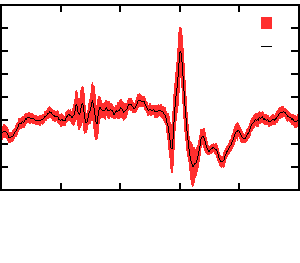
\includegraphics{voltage_0_108_gap_between_pulses_150_no_imaging_av_with_sd_means2_large2}}%
    \gplfronttext
  \end{picture}%
\endgroup
}\\
  \subfloat[1st pulse - \unit{250}\micro\second]{
    \label{fig:exp:control:av:time:250:detail:first}
    % GNUPLOT: LaTeX picture with Postscript
\begingroup
  \makeatletter
  \providecommand\color[2][]{%
    \GenericError{(gnuplot) \space\space\space\@spaces}{%
      Package color not loaded in conjunction with
      terminal option `colourtext'%
    }{See the gnuplot documentation for explanation.%
    }{Either use 'blacktext' in gnuplot or load the package
      color.sty in LaTeX.}%
    \renewcommand\color[2][]{}%
  }%
  \providecommand\includegraphics[2][]{%
    \GenericError{(gnuplot) \space\space\space\@spaces}{%
      Package graphicx or graphics not loaded%
    }{See the gnuplot documentation for explanation.%
    }{The gnuplot epslatex terminal needs graphicx.sty or graphics.sty.}%
    \renewcommand\includegraphics[2][]{}%
  }%
  \providecommand\rotatebox[2]{#2}%
  \@ifundefined{ifGPcolor}{%
    \newif\ifGPcolor
    \GPcolortrue
  }{}%
  \@ifundefined{ifGPblacktext}{%
    \newif\ifGPblacktext
    \GPblacktexttrue
  }{}%
  % define a \g@addto@macro without @ in the name:
  \let\gplgaddtomacro\g@addto@macro
  % define empty templates for all commands taking text:
  \gdef\gplbacktext{}%
  \gdef\gplfronttext{}%
  \makeatother
  \ifGPblacktext
    % no textcolor at all
    \def\colorrgb#1{}%
    \def\colorgray#1{}%
  \else
    % gray or color?
    \ifGPcolor
      \def\colorrgb#1{\color[rgb]{#1}}%
      \def\colorgray#1{\color[gray]{#1}}%
      \expandafter\def\csname LTw\endcsname{\color{white}}%
      \expandafter\def\csname LTb\endcsname{\color{black}}%
      \expandafter\def\csname LTa\endcsname{\color{black}}%
      \expandafter\def\csname LT0\endcsname{\color[rgb]{1,0,0}}%
      \expandafter\def\csname LT1\endcsname{\color[rgb]{0,1,0}}%
      \expandafter\def\csname LT2\endcsname{\color[rgb]{0,0,1}}%
      \expandafter\def\csname LT3\endcsname{\color[rgb]{1,0,1}}%
      \expandafter\def\csname LT4\endcsname{\color[rgb]{0,1,1}}%
      \expandafter\def\csname LT5\endcsname{\color[rgb]{1,1,0}}%
      \expandafter\def\csname LT6\endcsname{\color[rgb]{0,0,0}}%
      \expandafter\def\csname LT7\endcsname{\color[rgb]{1,0.3,0}}%
      \expandafter\def\csname LT8\endcsname{\color[rgb]{0.5,0.5,0.5}}%
    \else
      % gray
      \def\colorrgb#1{\color{black}}%
      \def\colorgray#1{\color[gray]{#1}}%
      \expandafter\def\csname LTw\endcsname{\color{white}}%
      \expandafter\def\csname LTb\endcsname{\color{black}}%
      \expandafter\def\csname LTa\endcsname{\color{black}}%
      \expandafter\def\csname LT0\endcsname{\color{black}}%
      \expandafter\def\csname LT1\endcsname{\color{black}}%
      \expandafter\def\csname LT2\endcsname{\color{black}}%
      \expandafter\def\csname LT3\endcsname{\color{black}}%
      \expandafter\def\csname LT4\endcsname{\color{black}}%
      \expandafter\def\csname LT5\endcsname{\color{black}}%
      \expandafter\def\csname LT6\endcsname{\color{black}}%
      \expandafter\def\csname LT7\endcsname{\color{black}}%
      \expandafter\def\csname LT8\endcsname{\color{black}}%
    \fi
  \fi
  \setlength{\unitlength}{0.0500bp}%
  \begin{picture}(2880.00,2520.00)%
    \gplgaddtomacro\gplbacktext{%
      \csname LTb\endcsname%
      \put(-119,704){\makebox(0,0)[r]{\strut{}-0.6}}%
      \put(-119,957){\makebox(0,0)[r]{\strut{}-0.4}}%
      \put(-119,1210){\makebox(0,0)[r]{\strut{}-0.2}}%
      \put(-119,1463){\makebox(0,0)[r]{\strut{} 0}}%
      \put(-119,1717){\makebox(0,0)[r]{\strut{} 0.2}}%
      \put(-119,1970){\makebox(0,0)[r]{\strut{} 0.4}}%
      \put(-119,2223){\makebox(0,0)[r]{\strut{} 0.6}}%
      \put(-119,2476){\makebox(0,0)[r]{\strut{} 0.8}}%
      \put(13,484){\makebox(0,0){\strut{} 17.5}}%
      \put(584,484){\makebox(0,0){\strut{} 18}}%
      \put(1154,484){\makebox(0,0){\strut{} 18.5}}%
      \put(1725,484){\makebox(0,0){\strut{} 19}}%
      \put(2295,484){\makebox(0,0){\strut{} 19.5}}%
      \put(2866,484){\makebox(0,0){\strut{} 20}}%
      \put(-889,1590){\rotatebox{-270}{\makebox(0,0){\strut{}voltage (V)}}}%
      \put(1439,154){\makebox(0,0){\strut{}time ($\mu$ s)}}%
    }%
    \gplgaddtomacro\gplfronttext{%
      \csname LTb\endcsname%
      \put(2381,2303){\makebox(0,0)[r]{\strut{}1-$\sigma$}}%
      \csname LTb\endcsname%
      \put(2381,2083){\makebox(0,0)[r]{\strut{}av.}}%
    }%
    \gplbacktext
    \put(0,0){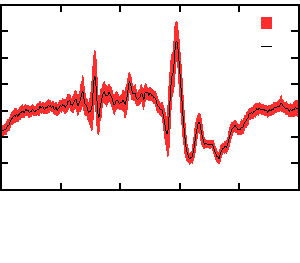
\includegraphics{voltage_0_108_gap_between_pulses_250_no_imaging_av_with_sd_means1_large2}}%
    \gplfronttext
  \end{picture}%
\endgroup
}
 \quad
  \subfloat[2nd pulse - \unit{250}\micro\second]{
    \label{fig:exp:control:av:time:250:detail:second}
    % GNUPLOT: LaTeX picture with Postscript
\begingroup
  \makeatletter
  \providecommand\color[2][]{%
    \GenericError{(gnuplot) \space\space\space\@spaces}{%
      Package color not loaded in conjunction with
      terminal option `colourtext'%
    }{See the gnuplot documentation for explanation.%
    }{Either use 'blacktext' in gnuplot or load the package
      color.sty in LaTeX.}%
    \renewcommand\color[2][]{}%
  }%
  \providecommand\includegraphics[2][]{%
    \GenericError{(gnuplot) \space\space\space\@spaces}{%
      Package graphicx or graphics not loaded%
    }{See the gnuplot documentation for explanation.%
    }{The gnuplot epslatex terminal needs graphicx.sty or graphics.sty.}%
    \renewcommand\includegraphics[2][]{}%
  }%
  \providecommand\rotatebox[2]{#2}%
  \@ifundefined{ifGPcolor}{%
    \newif\ifGPcolor
    \GPcolortrue
  }{}%
  \@ifundefined{ifGPblacktext}{%
    \newif\ifGPblacktext
    \GPblacktexttrue
  }{}%
  % define a \g@addto@macro without @ in the name:
  \let\gplgaddtomacro\g@addto@macro
  % define empty templates for all commands taking text:
  \gdef\gplbacktext{}%
  \gdef\gplfronttext{}%
  \makeatother
  \ifGPblacktext
    % no textcolor at all
    \def\colorrgb#1{}%
    \def\colorgray#1{}%
  \else
    % gray or color?
    \ifGPcolor
      \def\colorrgb#1{\color[rgb]{#1}}%
      \def\colorgray#1{\color[gray]{#1}}%
      \expandafter\def\csname LTw\endcsname{\color{white}}%
      \expandafter\def\csname LTb\endcsname{\color{black}}%
      \expandafter\def\csname LTa\endcsname{\color{black}}%
      \expandafter\def\csname LT0\endcsname{\color[rgb]{1,0,0}}%
      \expandafter\def\csname LT1\endcsname{\color[rgb]{0,1,0}}%
      \expandafter\def\csname LT2\endcsname{\color[rgb]{0,0,1}}%
      \expandafter\def\csname LT3\endcsname{\color[rgb]{1,0,1}}%
      \expandafter\def\csname LT4\endcsname{\color[rgb]{0,1,1}}%
      \expandafter\def\csname LT5\endcsname{\color[rgb]{1,1,0}}%
      \expandafter\def\csname LT6\endcsname{\color[rgb]{0,0,0}}%
      \expandafter\def\csname LT7\endcsname{\color[rgb]{1,0.3,0}}%
      \expandafter\def\csname LT8\endcsname{\color[rgb]{0.5,0.5,0.5}}%
    \else
      % gray
      \def\colorrgb#1{\color{black}}%
      \def\colorgray#1{\color[gray]{#1}}%
      \expandafter\def\csname LTw\endcsname{\color{white}}%
      \expandafter\def\csname LTb\endcsname{\color{black}}%
      \expandafter\def\csname LTa\endcsname{\color{black}}%
      \expandafter\def\csname LT0\endcsname{\color{black}}%
      \expandafter\def\csname LT1\endcsname{\color{black}}%
      \expandafter\def\csname LT2\endcsname{\color{black}}%
      \expandafter\def\csname LT3\endcsname{\color{black}}%
      \expandafter\def\csname LT4\endcsname{\color{black}}%
      \expandafter\def\csname LT5\endcsname{\color{black}}%
      \expandafter\def\csname LT6\endcsname{\color{black}}%
      \expandafter\def\csname LT7\endcsname{\color{black}}%
      \expandafter\def\csname LT8\endcsname{\color{black}}%
    \fi
  \fi
  \setlength{\unitlength}{0.0500bp}%
  \begin{picture}(2880.00,2520.00)%
    \gplgaddtomacro\gplbacktext{%
      \csname LTb\endcsname%
      \put(-119,704){\makebox(0,0)[r]{\strut{}}}%
      \put(-119,926){\makebox(0,0)[r]{\strut{}}}%
      \put(-119,1147){\makebox(0,0)[r]{\strut{}}}%
      \put(-119,1369){\makebox(0,0)[r]{\strut{}}}%
      \put(-119,1590){\makebox(0,0)[r]{\strut{}}}%
      \put(-119,1812){\makebox(0,0)[r]{\strut{}}}%
      \put(-119,2033){\makebox(0,0)[r]{\strut{}}}%
      \put(-119,2255){\makebox(0,0)[r]{\strut{}}}%
      \put(-119,2476){\makebox(0,0)[r]{\strut{}}}%
      \put(13,484){\makebox(0,0){\strut{} 17.5}}%
      \put(584,484){\makebox(0,0){\strut{} 18}}%
      \put(1154,484){\makebox(0,0){\strut{} 18.5}}%
      \put(1725,484){\makebox(0,0){\strut{} 19}}%
      \put(2295,484){\makebox(0,0){\strut{} 19.5}}%
      \put(2866,484){\makebox(0,0){\strut{} 20}}%
      \put(1439,154){\makebox(0,0){\strut{}time ($\mu$ s)}}%
    }%
    \gplgaddtomacro\gplfronttext{%
      \csname LTb\endcsname%
      \put(2381,2303){\makebox(0,0)[r]{\strut{}1-$\sigma$}}%
      \csname LTb\endcsname%
      \put(2381,2083){\makebox(0,0)[r]{\strut{}av.}}%
    }%
    \gplbacktext
    \put(0,0){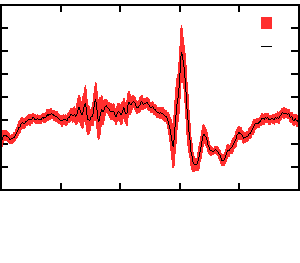
\includegraphics{voltage_0_108_gap_between_pulses_250_no_imaging_av_with_sd_means2_large2}}%
    \gplfronttext
  \end{picture}%
\endgroup
}
\caption{
    The receive only plots of \figref{exp:control:av:time} in greater detail.
  }
  \label{fig:exp:control:av:time:detail}
\end{figure}

The results are somewhat disappointing.
The two driving pulses do not cancel as hoped.
Rather, the strong scatter from the bubble has been accentuated.
To understand why, \figref{exp:control:av:time} is plotted in greater detail in \figref{exp:control:av:time:detail}
It is seen in \figref{exp:control:av:time:detail} that the second pulse,
although similar in shape to the first,
is shifted in phase by a small fraction of a microsecond.
%This prevents the cancellation between the waves.
%When calculated as a fraction of the driving wave,
%the phase shift evaluates to a approximately ...  \todo{evaluate}.
%The phase shift between the two pulses is indicative 
%of the slightly different bubble environments that exist between the two pulses.
%From \eqnref{} we estimate the bubbles to be a \todo{evaluate} further away from resonance.
%
The phase shift makes it possible to estimate
the change in the bubble environment between adjacent pulses,
but we do not pursue this here.
Instead, 
we will modify our approach to excess imaging slightly.
Rather than subtracting the second pulse from the first,
where the bubble populations are demonstrably different,
we will group the experimental results 
from the first pulse and the second pulse separately.
That is, 
the receive only image for the first driving pulse will
be compared to the pulse-echo image of the first driving pulse.
Likewise,
the receive-only image for the second pulse will be compared with
the pulse echo image that samples that second pulse.


%we attempt to remove the phase shift by adding a lag when processing the data
%to the first pulse so that it more closely overlaps with the second.
%The lag is evaluated by cross correlation.

%The lag-corrected cross-correlation is shown in figref{},
%and performs more satisfactory according to the requirements of excess pressure imaging.

% \begin{figure}[t]%
%   \centering
%   \subfloat[1st pulse - 100]{
%     \label{fig:av:108:100_ex:first}
%     % GNUPLOT: LaTeX picture with Postscript
\begingroup
  \makeatletter
  \providecommand\color[2][]{%
    \GenericError{(gnuplot) \space\space\space\@spaces}{%
      Package color not loaded in conjunction with
      terminal option `colourtext'%
    }{See the gnuplot documentation for explanation.%
    }{Either use 'blacktext' in gnuplot or load the package
      color.sty in LaTeX.}%
    \renewcommand\color[2][]{}%
  }%
  \providecommand\includegraphics[2][]{%
    \GenericError{(gnuplot) \space\space\space\@spaces}{%
      Package graphicx or graphics not loaded%
    }{See the gnuplot documentation for explanation.%
    }{The gnuplot epslatex terminal needs graphicx.sty or graphics.sty.}%
    \renewcommand\includegraphics[2][]{}%
  }%
  \providecommand\rotatebox[2]{#2}%
  \@ifundefined{ifGPcolor}{%
    \newif\ifGPcolor
    \GPcolortrue
  }{}%
  \@ifundefined{ifGPblacktext}{%
    \newif\ifGPblacktext
    \GPblacktexttrue
  }{}%
  % define a \g@addto@macro without @ in the name:
  \let\gplgaddtomacro\g@addto@macro
  % define empty templates for all commands taking text:
  \gdef\gplbacktext{}%
  \gdef\gplfronttext{}%
  \makeatother
  \ifGPblacktext
    % no textcolor at all
    \def\colorrgb#1{}%
    \def\colorgray#1{}%
  \else
    % gray or color?
    \ifGPcolor
      \def\colorrgb#1{\color[rgb]{#1}}%
      \def\colorgray#1{\color[gray]{#1}}%
      \expandafter\def\csname LTw\endcsname{\color{white}}%
      \expandafter\def\csname LTb\endcsname{\color{black}}%
      \expandafter\def\csname LTa\endcsname{\color{black}}%
      \expandafter\def\csname LT0\endcsname{\color[rgb]{1,0,0}}%
      \expandafter\def\csname LT1\endcsname{\color[rgb]{0,1,0}}%
      \expandafter\def\csname LT2\endcsname{\color[rgb]{0,0,1}}%
      \expandafter\def\csname LT3\endcsname{\color[rgb]{1,0,1}}%
      \expandafter\def\csname LT4\endcsname{\color[rgb]{0,1,1}}%
      \expandafter\def\csname LT5\endcsname{\color[rgb]{1,1,0}}%
      \expandafter\def\csname LT6\endcsname{\color[rgb]{0,0,0}}%
      \expandafter\def\csname LT7\endcsname{\color[rgb]{1,0.3,0}}%
      \expandafter\def\csname LT8\endcsname{\color[rgb]{0.5,0.5,0.5}}%
    \else
      % gray
      \def\colorrgb#1{\color{black}}%
      \def\colorgray#1{\color[gray]{#1}}%
      \expandafter\def\csname LTw\endcsname{\color{white}}%
      \expandafter\def\csname LTb\endcsname{\color{black}}%
      \expandafter\def\csname LTa\endcsname{\color{black}}%
      \expandafter\def\csname LT0\endcsname{\color{black}}%
      \expandafter\def\csname LT1\endcsname{\color{black}}%
      \expandafter\def\csname LT2\endcsname{\color{black}}%
      \expandafter\def\csname LT3\endcsname{\color{black}}%
      \expandafter\def\csname LT4\endcsname{\color{black}}%
      \expandafter\def\csname LT5\endcsname{\color{black}}%
      \expandafter\def\csname LT6\endcsname{\color{black}}%
      \expandafter\def\csname LT7\endcsname{\color{black}}%
      \expandafter\def\csname LT8\endcsname{\color{black}}%
    \fi
  \fi
  \setlength{\unitlength}{0.0500bp}%
  \begin{picture}(2880.00,2520.00)%
    \gplgaddtomacro\gplbacktext{%
      \csname LTb\endcsname%
      \put(-119,704){\makebox(0,0)[r]{\strut{}-1}}%
      \put(-119,1058){\makebox(0,0)[r]{\strut{}-0.5}}%
      \put(-119,1413){\makebox(0,0)[r]{\strut{} 0}}%
      \put(-119,1767){\makebox(0,0)[r]{\strut{} 0.5}}%
      \put(-119,2122){\makebox(0,0)[r]{\strut{} 1}}%
      \put(-119,2476){\makebox(0,0)[r]{\strut{} 1.5}}%
      \put(13,484){\makebox(0,0){\strut{} 0}}%
      \put(421,484){\makebox(0,0){\strut{} 5}}%
      \put(828,484){\makebox(0,0){\strut{} 10}}%
      \put(1236,484){\makebox(0,0){\strut{} 15}}%
      \put(1643,484){\makebox(0,0){\strut{} 20}}%
      \put(2051,484){\makebox(0,0){\strut{} 25}}%
      \put(2458,484){\makebox(0,0){\strut{} 30}}%
      \put(2866,484){\makebox(0,0){\strut{} 35}}%
      \put(-889,1590){\rotatebox{-270}{\makebox(0,0){\strut{}voltage (V)}}}%
      \put(1439,154){\makebox(0,0){\strut{}time ($\mu$ s)}}%
    }%
    \gplgaddtomacro\gplfronttext{%
      \csname LTb\endcsname%
      \put(2381,2303){\makebox(0,0)[r]{\strut{}1-$\sigma$}}%
      \csname LTb\endcsname%
      \put(2381,2083){\makebox(0,0)[r]{\strut{}av.}}%
    }%
    \gplbacktext
    \put(0,0){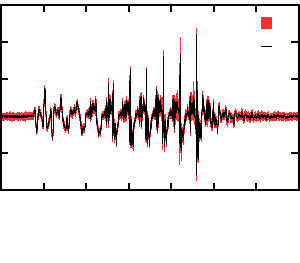
\includegraphics{voltage_0_108_gap_between_pulses_100_imaging_1st_av_with_sd_means1_large}}%
    \gplfronttext
  \end{picture}%
\endgroup
}
%  \quad
%   \subfloat[2nd pulse - 100]{
%     \label{fig:av:108:100_ex:second}
%     % GNUPLOT: LaTeX picture with Postscript
\begingroup
  \makeatletter
  \providecommand\color[2][]{%
    \GenericError{(gnuplot) \space\space\space\@spaces}{%
      Package color not loaded in conjunction with
      terminal option `colourtext'%
    }{See the gnuplot documentation for explanation.%
    }{Either use 'blacktext' in gnuplot or load the package
      color.sty in LaTeX.}%
    \renewcommand\color[2][]{}%
  }%
  \providecommand\includegraphics[2][]{%
    \GenericError{(gnuplot) \space\space\space\@spaces}{%
      Package graphicx or graphics not loaded%
    }{See the gnuplot documentation for explanation.%
    }{The gnuplot epslatex terminal needs graphicx.sty or graphics.sty.}%
    \renewcommand\includegraphics[2][]{}%
  }%
  \providecommand\rotatebox[2]{#2}%
  \@ifundefined{ifGPcolor}{%
    \newif\ifGPcolor
    \GPcolortrue
  }{}%
  \@ifundefined{ifGPblacktext}{%
    \newif\ifGPblacktext
    \GPblacktexttrue
  }{}%
  % define a \g@addto@macro without @ in the name:
  \let\gplgaddtomacro\g@addto@macro
  % define empty templates for all commands taking text:
  \gdef\gplbacktext{}%
  \gdef\gplfronttext{}%
  \makeatother
  \ifGPblacktext
    % no textcolor at all
    \def\colorrgb#1{}%
    \def\colorgray#1{}%
  \else
    % gray or color?
    \ifGPcolor
      \def\colorrgb#1{\color[rgb]{#1}}%
      \def\colorgray#1{\color[gray]{#1}}%
      \expandafter\def\csname LTw\endcsname{\color{white}}%
      \expandafter\def\csname LTb\endcsname{\color{black}}%
      \expandafter\def\csname LTa\endcsname{\color{black}}%
      \expandafter\def\csname LT0\endcsname{\color[rgb]{1,0,0}}%
      \expandafter\def\csname LT1\endcsname{\color[rgb]{0,1,0}}%
      \expandafter\def\csname LT2\endcsname{\color[rgb]{0,0,1}}%
      \expandafter\def\csname LT3\endcsname{\color[rgb]{1,0,1}}%
      \expandafter\def\csname LT4\endcsname{\color[rgb]{0,1,1}}%
      \expandafter\def\csname LT5\endcsname{\color[rgb]{1,1,0}}%
      \expandafter\def\csname LT6\endcsname{\color[rgb]{0,0,0}}%
      \expandafter\def\csname LT7\endcsname{\color[rgb]{1,0.3,0}}%
      \expandafter\def\csname LT8\endcsname{\color[rgb]{0.5,0.5,0.5}}%
    \else
      % gray
      \def\colorrgb#1{\color{black}}%
      \def\colorgray#1{\color[gray]{#1}}%
      \expandafter\def\csname LTw\endcsname{\color{white}}%
      \expandafter\def\csname LTb\endcsname{\color{black}}%
      \expandafter\def\csname LTa\endcsname{\color{black}}%
      \expandafter\def\csname LT0\endcsname{\color{black}}%
      \expandafter\def\csname LT1\endcsname{\color{black}}%
      \expandafter\def\csname LT2\endcsname{\color{black}}%
      \expandafter\def\csname LT3\endcsname{\color{black}}%
      \expandafter\def\csname LT4\endcsname{\color{black}}%
      \expandafter\def\csname LT5\endcsname{\color{black}}%
      \expandafter\def\csname LT6\endcsname{\color{black}}%
      \expandafter\def\csname LT7\endcsname{\color{black}}%
      \expandafter\def\csname LT8\endcsname{\color{black}}%
    \fi
  \fi
  \setlength{\unitlength}{0.0500bp}%
  \begin{picture}(2880.00,2520.00)%
    \gplgaddtomacro\gplbacktext{%
      \csname LTb\endcsname%
      \put(-119,704){\makebox(0,0)[r]{\strut{}}}%
      \put(-119,881){\makebox(0,0)[r]{\strut{}}}%
      \put(-119,1058){\makebox(0,0)[r]{\strut{}}}%
      \put(-119,1236){\makebox(0,0)[r]{\strut{}}}%
      \put(-119,1413){\makebox(0,0)[r]{\strut{}}}%
      \put(-119,1590){\makebox(0,0)[r]{\strut{}}}%
      \put(-119,1767){\makebox(0,0)[r]{\strut{}}}%
      \put(-119,1944){\makebox(0,0)[r]{\strut{}}}%
      \put(-119,2122){\makebox(0,0)[r]{\strut{}}}%
      \put(-119,2299){\makebox(0,0)[r]{\strut{}}}%
      \put(-119,2476){\makebox(0,0)[r]{\strut{}}}%
      \put(13,484){\makebox(0,0){\strut{} 0}}%
      \put(421,484){\makebox(0,0){\strut{} 5}}%
      \put(828,484){\makebox(0,0){\strut{} 10}}%
      \put(1236,484){\makebox(0,0){\strut{} 15}}%
      \put(1643,484){\makebox(0,0){\strut{} 20}}%
      \put(2051,484){\makebox(0,0){\strut{} 25}}%
      \put(2458,484){\makebox(0,0){\strut{} 30}}%
      \put(2866,484){\makebox(0,0){\strut{} 35}}%
      \put(1439,154){\makebox(0,0){\strut{}time ($\mu$ s)}}%
    }%
    \gplgaddtomacro\gplfronttext{%
      \csname LTb\endcsname%
      \put(2381,2303){\makebox(0,0)[r]{\strut{}1-$\sigma$}}%
      \csname LTb\endcsname%
      \put(2381,2083){\makebox(0,0)[r]{\strut{}av.}}%
    }%
    \gplbacktext
    \put(0,0){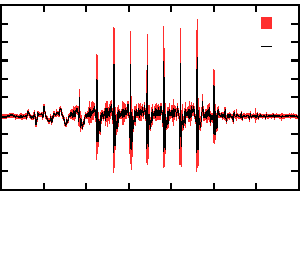
\includegraphics{voltage_0_108_gap_between_pulses_100_imaging_1st_av_with_sd_means2_large}}%
    \gplfronttext
  \end{picture}%
\endgroup
}\\
%   \subfloat[1st pulse - 150]{
%     \label{fig:av:108:100_ex:first}
%     % GNUPLOT: LaTeX picture with Postscript
\begingroup
  \makeatletter
  \providecommand\color[2][]{%
    \GenericError{(gnuplot) \space\space\space\@spaces}{%
      Package color not loaded in conjunction with
      terminal option `colourtext'%
    }{See the gnuplot documentation for explanation.%
    }{Either use 'blacktext' in gnuplot or load the package
      color.sty in LaTeX.}%
    \renewcommand\color[2][]{}%
  }%
  \providecommand\includegraphics[2][]{%
    \GenericError{(gnuplot) \space\space\space\@spaces}{%
      Package graphicx or graphics not loaded%
    }{See the gnuplot documentation for explanation.%
    }{The gnuplot epslatex terminal needs graphicx.sty or graphics.sty.}%
    \renewcommand\includegraphics[2][]{}%
  }%
  \providecommand\rotatebox[2]{#2}%
  \@ifundefined{ifGPcolor}{%
    \newif\ifGPcolor
    \GPcolortrue
  }{}%
  \@ifundefined{ifGPblacktext}{%
    \newif\ifGPblacktext
    \GPblacktexttrue
  }{}%
  % define a \g@addto@macro without @ in the name:
  \let\gplgaddtomacro\g@addto@macro
  % define empty templates for all commands taking text:
  \gdef\gplbacktext{}%
  \gdef\gplfronttext{}%
  \makeatother
  \ifGPblacktext
    % no textcolor at all
    \def\colorrgb#1{}%
    \def\colorgray#1{}%
  \else
    % gray or color?
    \ifGPcolor
      \def\colorrgb#1{\color[rgb]{#1}}%
      \def\colorgray#1{\color[gray]{#1}}%
      \expandafter\def\csname LTw\endcsname{\color{white}}%
      \expandafter\def\csname LTb\endcsname{\color{black}}%
      \expandafter\def\csname LTa\endcsname{\color{black}}%
      \expandafter\def\csname LT0\endcsname{\color[rgb]{1,0,0}}%
      \expandafter\def\csname LT1\endcsname{\color[rgb]{0,1,0}}%
      \expandafter\def\csname LT2\endcsname{\color[rgb]{0,0,1}}%
      \expandafter\def\csname LT3\endcsname{\color[rgb]{1,0,1}}%
      \expandafter\def\csname LT4\endcsname{\color[rgb]{0,1,1}}%
      \expandafter\def\csname LT5\endcsname{\color[rgb]{1,1,0}}%
      \expandafter\def\csname LT6\endcsname{\color[rgb]{0,0,0}}%
      \expandafter\def\csname LT7\endcsname{\color[rgb]{1,0.3,0}}%
      \expandafter\def\csname LT8\endcsname{\color[rgb]{0.5,0.5,0.5}}%
    \else
      % gray
      \def\colorrgb#1{\color{black}}%
      \def\colorgray#1{\color[gray]{#1}}%
      \expandafter\def\csname LTw\endcsname{\color{white}}%
      \expandafter\def\csname LTb\endcsname{\color{black}}%
      \expandafter\def\csname LTa\endcsname{\color{black}}%
      \expandafter\def\csname LT0\endcsname{\color{black}}%
      \expandafter\def\csname LT1\endcsname{\color{black}}%
      \expandafter\def\csname LT2\endcsname{\color{black}}%
      \expandafter\def\csname LT3\endcsname{\color{black}}%
      \expandafter\def\csname LT4\endcsname{\color{black}}%
      \expandafter\def\csname LT5\endcsname{\color{black}}%
      \expandafter\def\csname LT6\endcsname{\color{black}}%
      \expandafter\def\csname LT7\endcsname{\color{black}}%
      \expandafter\def\csname LT8\endcsname{\color{black}}%
    \fi
  \fi
  \setlength{\unitlength}{0.0500bp}%
  \begin{picture}(2880.00,2520.00)%
    \gplgaddtomacro\gplbacktext{%
      \csname LTb\endcsname%
      \put(-119,704){\makebox(0,0)[r]{\strut{}-0.6}}%
      \put(-119,957){\makebox(0,0)[r]{\strut{}-0.4}}%
      \put(-119,1210){\makebox(0,0)[r]{\strut{}-0.2}}%
      \put(-119,1463){\makebox(0,0)[r]{\strut{} 0}}%
      \put(-119,1717){\makebox(0,0)[r]{\strut{} 0.2}}%
      \put(-119,1970){\makebox(0,0)[r]{\strut{} 0.4}}%
      \put(-119,2223){\makebox(0,0)[r]{\strut{} 0.6}}%
      \put(-119,2476){\makebox(0,0)[r]{\strut{} 0.8}}%
      \put(13,484){\makebox(0,0){\strut{} 0}}%
      \put(421,484){\makebox(0,0){\strut{} 5}}%
      \put(828,484){\makebox(0,0){\strut{} 10}}%
      \put(1236,484){\makebox(0,0){\strut{} 15}}%
      \put(1643,484){\makebox(0,0){\strut{} 20}}%
      \put(2051,484){\makebox(0,0){\strut{} 25}}%
      \put(2458,484){\makebox(0,0){\strut{} 30}}%
      \put(2866,484){\makebox(0,0){\strut{} 35}}%
      \put(-889,1590){\rotatebox{-270}{\makebox(0,0){\strut{}voltage (V)}}}%
      \put(1439,154){\makebox(0,0){\strut{}time ($\mu$ s)}}%
    }%
    \gplgaddtomacro\gplfronttext{%
      \csname LTb\endcsname%
      \put(2381,2303){\makebox(0,0)[r]{\strut{}1-$\sigma$}}%
      \csname LTb\endcsname%
      \put(2381,2083){\makebox(0,0)[r]{\strut{}av.}}%
    }%
    \gplbacktext
    \put(0,0){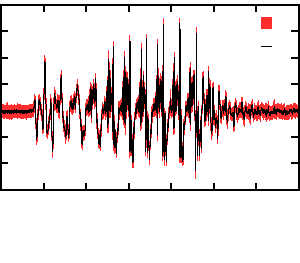
\includegraphics{voltage_0_108_gap_between_pulses_150_imaging_1st_av_with_sd_means1_large}}%
    \gplfronttext
  \end{picture}%
\endgroup
}
%  \quad
%   \subfloat[2nd pulse - 150]{
%     \label{fig:av:108:100_ex:second}
%     % GNUPLOT: LaTeX picture with Postscript
\begingroup
  \makeatletter
  \providecommand\color[2][]{%
    \GenericError{(gnuplot) \space\space\space\@spaces}{%
      Package color not loaded in conjunction with
      terminal option `colourtext'%
    }{See the gnuplot documentation for explanation.%
    }{Either use 'blacktext' in gnuplot or load the package
      color.sty in LaTeX.}%
    \renewcommand\color[2][]{}%
  }%
  \providecommand\includegraphics[2][]{%
    \GenericError{(gnuplot) \space\space\space\@spaces}{%
      Package graphicx or graphics not loaded%
    }{See the gnuplot documentation for explanation.%
    }{The gnuplot epslatex terminal needs graphicx.sty or graphics.sty.}%
    \renewcommand\includegraphics[2][]{}%
  }%
  \providecommand\rotatebox[2]{#2}%
  \@ifundefined{ifGPcolor}{%
    \newif\ifGPcolor
    \GPcolortrue
  }{}%
  \@ifundefined{ifGPblacktext}{%
    \newif\ifGPblacktext
    \GPblacktexttrue
  }{}%
  % define a \g@addto@macro without @ in the name:
  \let\gplgaddtomacro\g@addto@macro
  % define empty templates for all commands taking text:
  \gdef\gplbacktext{}%
  \gdef\gplfronttext{}%
  \makeatother
  \ifGPblacktext
    % no textcolor at all
    \def\colorrgb#1{}%
    \def\colorgray#1{}%
  \else
    % gray or color?
    \ifGPcolor
      \def\colorrgb#1{\color[rgb]{#1}}%
      \def\colorgray#1{\color[gray]{#1}}%
      \expandafter\def\csname LTw\endcsname{\color{white}}%
      \expandafter\def\csname LTb\endcsname{\color{black}}%
      \expandafter\def\csname LTa\endcsname{\color{black}}%
      \expandafter\def\csname LT0\endcsname{\color[rgb]{1,0,0}}%
      \expandafter\def\csname LT1\endcsname{\color[rgb]{0,1,0}}%
      \expandafter\def\csname LT2\endcsname{\color[rgb]{0,0,1}}%
      \expandafter\def\csname LT3\endcsname{\color[rgb]{1,0,1}}%
      \expandafter\def\csname LT4\endcsname{\color[rgb]{0,1,1}}%
      \expandafter\def\csname LT5\endcsname{\color[rgb]{1,1,0}}%
      \expandafter\def\csname LT6\endcsname{\color[rgb]{0,0,0}}%
      \expandafter\def\csname LT7\endcsname{\color[rgb]{1,0.3,0}}%
      \expandafter\def\csname LT8\endcsname{\color[rgb]{0.5,0.5,0.5}}%
    \else
      % gray
      \def\colorrgb#1{\color{black}}%
      \def\colorgray#1{\color[gray]{#1}}%
      \expandafter\def\csname LTw\endcsname{\color{white}}%
      \expandafter\def\csname LTb\endcsname{\color{black}}%
      \expandafter\def\csname LTa\endcsname{\color{black}}%
      \expandafter\def\csname LT0\endcsname{\color{black}}%
      \expandafter\def\csname LT1\endcsname{\color{black}}%
      \expandafter\def\csname LT2\endcsname{\color{black}}%
      \expandafter\def\csname LT3\endcsname{\color{black}}%
      \expandafter\def\csname LT4\endcsname{\color{black}}%
      \expandafter\def\csname LT5\endcsname{\color{black}}%
      \expandafter\def\csname LT6\endcsname{\color{black}}%
      \expandafter\def\csname LT7\endcsname{\color{black}}%
      \expandafter\def\csname LT8\endcsname{\color{black}}%
    \fi
  \fi
  \setlength{\unitlength}{0.0500bp}%
  \begin{picture}(2880.00,2520.00)%
    \gplgaddtomacro\gplbacktext{%
      \csname LTb\endcsname%
      \put(-119,704){\makebox(0,0)[r]{\strut{}}}%
      \put(-119,901){\makebox(0,0)[r]{\strut{}}}%
      \put(-119,1098){\makebox(0,0)[r]{\strut{}}}%
      \put(-119,1295){\makebox(0,0)[r]{\strut{}}}%
      \put(-119,1492){\makebox(0,0)[r]{\strut{}}}%
      \put(-119,1688){\makebox(0,0)[r]{\strut{}}}%
      \put(-119,1885){\makebox(0,0)[r]{\strut{}}}%
      \put(-119,2082){\makebox(0,0)[r]{\strut{}}}%
      \put(-119,2279){\makebox(0,0)[r]{\strut{}}}%
      \put(-119,2476){\makebox(0,0)[r]{\strut{}}}%
      \put(13,484){\makebox(0,0){\strut{} 0}}%
      \put(421,484){\makebox(0,0){\strut{} 5}}%
      \put(828,484){\makebox(0,0){\strut{} 10}}%
      \put(1236,484){\makebox(0,0){\strut{} 15}}%
      \put(1643,484){\makebox(0,0){\strut{} 20}}%
      \put(2051,484){\makebox(0,0){\strut{} 25}}%
      \put(2458,484){\makebox(0,0){\strut{} 30}}%
      \put(2866,484){\makebox(0,0){\strut{} 35}}%
      \put(1439,154){\makebox(0,0){\strut{}time ($\mu$ s)}}%
    }%
    \gplgaddtomacro\gplfronttext{%
      \csname LTb\endcsname%
      \put(2381,2303){\makebox(0,0)[r]{\strut{}1-$\sigma$}}%
      \csname LTb\endcsname%
      \put(2381,2083){\makebox(0,0)[r]{\strut{}av.}}%
    }%
    \gplbacktext
    \put(0,0){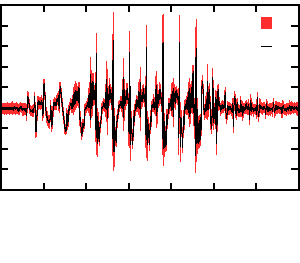
\includegraphics{voltage_0_108_gap_between_pulses_150_imaging_1st_av_with_sd_means2_large}}%
    \gplfronttext
  \end{picture}%
\endgroup
}\\
%   \subfloat[1st pulse - 250]{
%     \label{fig:av:108:100_ex:first}
%     % GNUPLOT: LaTeX picture with Postscript
\begingroup
  \makeatletter
  \providecommand\color[2][]{%
    \GenericError{(gnuplot) \space\space\space\@spaces}{%
      Package color not loaded in conjunction with
      terminal option `colourtext'%
    }{See the gnuplot documentation for explanation.%
    }{Either use 'blacktext' in gnuplot or load the package
      color.sty in LaTeX.}%
    \renewcommand\color[2][]{}%
  }%
  \providecommand\includegraphics[2][]{%
    \GenericError{(gnuplot) \space\space\space\@spaces}{%
      Package graphicx or graphics not loaded%
    }{See the gnuplot documentation for explanation.%
    }{The gnuplot epslatex terminal needs graphicx.sty or graphics.sty.}%
    \renewcommand\includegraphics[2][]{}%
  }%
  \providecommand\rotatebox[2]{#2}%
  \@ifundefined{ifGPcolor}{%
    \newif\ifGPcolor
    \GPcolortrue
  }{}%
  \@ifundefined{ifGPblacktext}{%
    \newif\ifGPblacktext
    \GPblacktexttrue
  }{}%
  % define a \g@addto@macro without @ in the name:
  \let\gplgaddtomacro\g@addto@macro
  % define empty templates for all commands taking text:
  \gdef\gplbacktext{}%
  \gdef\gplfronttext{}%
  \makeatother
  \ifGPblacktext
    % no textcolor at all
    \def\colorrgb#1{}%
    \def\colorgray#1{}%
  \else
    % gray or color?
    \ifGPcolor
      \def\colorrgb#1{\color[rgb]{#1}}%
      \def\colorgray#1{\color[gray]{#1}}%
      \expandafter\def\csname LTw\endcsname{\color{white}}%
      \expandafter\def\csname LTb\endcsname{\color{black}}%
      \expandafter\def\csname LTa\endcsname{\color{black}}%
      \expandafter\def\csname LT0\endcsname{\color[rgb]{1,0,0}}%
      \expandafter\def\csname LT1\endcsname{\color[rgb]{0,1,0}}%
      \expandafter\def\csname LT2\endcsname{\color[rgb]{0,0,1}}%
      \expandafter\def\csname LT3\endcsname{\color[rgb]{1,0,1}}%
      \expandafter\def\csname LT4\endcsname{\color[rgb]{0,1,1}}%
      \expandafter\def\csname LT5\endcsname{\color[rgb]{1,1,0}}%
      \expandafter\def\csname LT6\endcsname{\color[rgb]{0,0,0}}%
      \expandafter\def\csname LT7\endcsname{\color[rgb]{1,0.3,0}}%
      \expandafter\def\csname LT8\endcsname{\color[rgb]{0.5,0.5,0.5}}%
    \else
      % gray
      \def\colorrgb#1{\color{black}}%
      \def\colorgray#1{\color[gray]{#1}}%
      \expandafter\def\csname LTw\endcsname{\color{white}}%
      \expandafter\def\csname LTb\endcsname{\color{black}}%
      \expandafter\def\csname LTa\endcsname{\color{black}}%
      \expandafter\def\csname LT0\endcsname{\color{black}}%
      \expandafter\def\csname LT1\endcsname{\color{black}}%
      \expandafter\def\csname LT2\endcsname{\color{black}}%
      \expandafter\def\csname LT3\endcsname{\color{black}}%
      \expandafter\def\csname LT4\endcsname{\color{black}}%
      \expandafter\def\csname LT5\endcsname{\color{black}}%
      \expandafter\def\csname LT6\endcsname{\color{black}}%
      \expandafter\def\csname LT7\endcsname{\color{black}}%
      \expandafter\def\csname LT8\endcsname{\color{black}}%
    \fi
  \fi
  \setlength{\unitlength}{0.0500bp}%
  \begin{picture}(2880.00,2520.00)%
    \gplgaddtomacro\gplbacktext{%
      \csname LTb\endcsname%
      \put(-119,704){\makebox(0,0)[r]{\strut{}-0.6}}%
      \put(-119,957){\makebox(0,0)[r]{\strut{}-0.4}}%
      \put(-119,1210){\makebox(0,0)[r]{\strut{}-0.2}}%
      \put(-119,1463){\makebox(0,0)[r]{\strut{} 0}}%
      \put(-119,1717){\makebox(0,0)[r]{\strut{} 0.2}}%
      \put(-119,1970){\makebox(0,0)[r]{\strut{} 0.4}}%
      \put(-119,2223){\makebox(0,0)[r]{\strut{} 0.6}}%
      \put(-119,2476){\makebox(0,0)[r]{\strut{} 0.8}}%
      \put(13,484){\makebox(0,0){\strut{} 0}}%
      \put(421,484){\makebox(0,0){\strut{} 5}}%
      \put(828,484){\makebox(0,0){\strut{} 10}}%
      \put(1236,484){\makebox(0,0){\strut{} 15}}%
      \put(1643,484){\makebox(0,0){\strut{} 20}}%
      \put(2051,484){\makebox(0,0){\strut{} 25}}%
      \put(2458,484){\makebox(0,0){\strut{} 30}}%
      \put(2866,484){\makebox(0,0){\strut{} 35}}%
      \put(-889,1590){\rotatebox{-270}{\makebox(0,0){\strut{}voltage (V)}}}%
      \put(1439,154){\makebox(0,0){\strut{}time ($\mu$ s)}}%
    }%
    \gplgaddtomacro\gplfronttext{%
      \csname LTb\endcsname%
      \put(2381,2303){\makebox(0,0)[r]{\strut{}1-$\sigma$}}%
      \csname LTb\endcsname%
      \put(2381,2083){\makebox(0,0)[r]{\strut{}av.}}%
    }%
    \gplbacktext
    \put(0,0){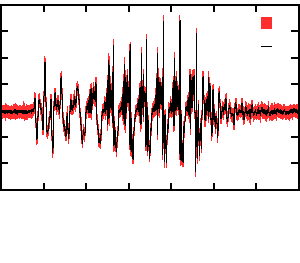
\includegraphics{voltage_0_108_gap_between_pulses_250_imaging_1st_av_with_sd_means1_large}}%
    \gplfronttext
  \end{picture}%
\endgroup
}
%  \quad
%   \subfloat[2nd pulse - 250]{
%     \label{fig:av:108:100_ex:second}
%     % GNUPLOT: LaTeX picture with Postscript
\begingroup
  \makeatletter
  \providecommand\color[2][]{%
    \GenericError{(gnuplot) \space\space\space\@spaces}{%
      Package color not loaded in conjunction with
      terminal option `colourtext'%
    }{See the gnuplot documentation for explanation.%
    }{Either use 'blacktext' in gnuplot or load the package
      color.sty in LaTeX.}%
    \renewcommand\color[2][]{}%
  }%
  \providecommand\includegraphics[2][]{%
    \GenericError{(gnuplot) \space\space\space\@spaces}{%
      Package graphicx or graphics not loaded%
    }{See the gnuplot documentation for explanation.%
    }{The gnuplot epslatex terminal needs graphicx.sty or graphics.sty.}%
    \renewcommand\includegraphics[2][]{}%
  }%
  \providecommand\rotatebox[2]{#2}%
  \@ifundefined{ifGPcolor}{%
    \newif\ifGPcolor
    \GPcolortrue
  }{}%
  \@ifundefined{ifGPblacktext}{%
    \newif\ifGPblacktext
    \GPblacktexttrue
  }{}%
  % define a \g@addto@macro without @ in the name:
  \let\gplgaddtomacro\g@addto@macro
  % define empty templates for all commands taking text:
  \gdef\gplbacktext{}%
  \gdef\gplfronttext{}%
  \makeatother
  \ifGPblacktext
    % no textcolor at all
    \def\colorrgb#1{}%
    \def\colorgray#1{}%
  \else
    % gray or color?
    \ifGPcolor
      \def\colorrgb#1{\color[rgb]{#1}}%
      \def\colorgray#1{\color[gray]{#1}}%
      \expandafter\def\csname LTw\endcsname{\color{white}}%
      \expandafter\def\csname LTb\endcsname{\color{black}}%
      \expandafter\def\csname LTa\endcsname{\color{black}}%
      \expandafter\def\csname LT0\endcsname{\color[rgb]{1,0,0}}%
      \expandafter\def\csname LT1\endcsname{\color[rgb]{0,1,0}}%
      \expandafter\def\csname LT2\endcsname{\color[rgb]{0,0,1}}%
      \expandafter\def\csname LT3\endcsname{\color[rgb]{1,0,1}}%
      \expandafter\def\csname LT4\endcsname{\color[rgb]{0,1,1}}%
      \expandafter\def\csname LT5\endcsname{\color[rgb]{1,1,0}}%
      \expandafter\def\csname LT6\endcsname{\color[rgb]{0,0,0}}%
      \expandafter\def\csname LT7\endcsname{\color[rgb]{1,0.3,0}}%
      \expandafter\def\csname LT8\endcsname{\color[rgb]{0.5,0.5,0.5}}%
    \else
      % gray
      \def\colorrgb#1{\color{black}}%
      \def\colorgray#1{\color[gray]{#1}}%
      \expandafter\def\csname LTw\endcsname{\color{white}}%
      \expandafter\def\csname LTb\endcsname{\color{black}}%
      \expandafter\def\csname LTa\endcsname{\color{black}}%
      \expandafter\def\csname LT0\endcsname{\color{black}}%
      \expandafter\def\csname LT1\endcsname{\color{black}}%
      \expandafter\def\csname LT2\endcsname{\color{black}}%
      \expandafter\def\csname LT3\endcsname{\color{black}}%
      \expandafter\def\csname LT4\endcsname{\color{black}}%
      \expandafter\def\csname LT5\endcsname{\color{black}}%
      \expandafter\def\csname LT6\endcsname{\color{black}}%
      \expandafter\def\csname LT7\endcsname{\color{black}}%
      \expandafter\def\csname LT8\endcsname{\color{black}}%
    \fi
  \fi
  \setlength{\unitlength}{0.0500bp}%
  \begin{picture}(2880.00,2520.00)%
    \gplgaddtomacro\gplbacktext{%
      \csname LTb\endcsname%
      \put(-119,704){\makebox(0,0)[r]{\strut{}}}%
      \put(-119,926){\makebox(0,0)[r]{\strut{}}}%
      \put(-119,1147){\makebox(0,0)[r]{\strut{}}}%
      \put(-119,1369){\makebox(0,0)[r]{\strut{}}}%
      \put(-119,1590){\makebox(0,0)[r]{\strut{}}}%
      \put(-119,1812){\makebox(0,0)[r]{\strut{}}}%
      \put(-119,2033){\makebox(0,0)[r]{\strut{}}}%
      \put(-119,2255){\makebox(0,0)[r]{\strut{}}}%
      \put(-119,2476){\makebox(0,0)[r]{\strut{}}}%
      \put(13,484){\makebox(0,0){\strut{} 0}}%
      \put(421,484){\makebox(0,0){\strut{} 5}}%
      \put(828,484){\makebox(0,0){\strut{} 10}}%
      \put(1236,484){\makebox(0,0){\strut{} 15}}%
      \put(1643,484){\makebox(0,0){\strut{} 20}}%
      \put(2051,484){\makebox(0,0){\strut{} 25}}%
      \put(2458,484){\makebox(0,0){\strut{} 30}}%
      \put(2866,484){\makebox(0,0){\strut{} 35}}%
      \put(1439,154){\makebox(0,0){\strut{}time ($\mu$ s)}}%
    }%
    \gplgaddtomacro\gplfronttext{%
      \csname LTb\endcsname%
      \put(2381,2303){\makebox(0,0)[r]{\strut{}1-$\sigma$}}%
      \csname LTb\endcsname%
      \put(2381,2083){\makebox(0,0)[r]{\strut{}av.}}%
    }%
    \gplbacktext
    \put(0,0){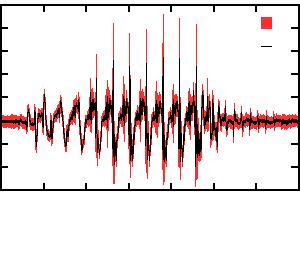
\includegraphics{voltage_0_108_gap_between_pulses_250_imaging_1st_av_with_sd_means2_large}}%
    \gplfronttext
  \end{picture}%
\endgroup
}
% \caption{
%     The pressure received  by the imaging transducer when the driving wave is on but the imaging wave is off (receive-only).
%     The second pulse \subref{fig:av:108:100:second} is received \unit{100}\micro\second\ after the first \subref{fig:av:108:100:first}.
%     Each image is the average of 49 images, the first standard-deviation error bars are indicated.
%   }
%   \label{fig:av:108:100_ex}
% \end{figure}



% \begin{figure}[t]%
%   \centering
%  \quad
%   \subfloat[2nd pulse - 100]{
%     \label{fig:av:108:100_ex:second}
%     % GNUPLOT: LaTeX picture with Postscript
\begingroup
  \makeatletter
  \providecommand\color[2][]{%
    \GenericError{(gnuplot) \space\space\space\@spaces}{%
      Package color not loaded in conjunction with
      terminal option `colourtext'%
    }{See the gnuplot documentation for explanation.%
    }{Either use 'blacktext' in gnuplot or load the package
      color.sty in LaTeX.}%
    \renewcommand\color[2][]{}%
  }%
  \providecommand\includegraphics[2][]{%
    \GenericError{(gnuplot) \space\space\space\@spaces}{%
      Package graphicx or graphics not loaded%
    }{See the gnuplot documentation for explanation.%
    }{The gnuplot epslatex terminal needs graphicx.sty or graphics.sty.}%
    \renewcommand\includegraphics[2][]{}%
  }%
  \providecommand\rotatebox[2]{#2}%
  \@ifundefined{ifGPcolor}{%
    \newif\ifGPcolor
    \GPcolortrue
  }{}%
  \@ifundefined{ifGPblacktext}{%
    \newif\ifGPblacktext
    \GPblacktexttrue
  }{}%
  % define a \g@addto@macro without @ in the name:
  \let\gplgaddtomacro\g@addto@macro
  % define empty templates for all commands taking text:
  \gdef\gplbacktext{}%
  \gdef\gplfronttext{}%
  \makeatother
  \ifGPblacktext
    % no textcolor at all
    \def\colorrgb#1{}%
    \def\colorgray#1{}%
  \else
    % gray or color?
    \ifGPcolor
      \def\colorrgb#1{\color[rgb]{#1}}%
      \def\colorgray#1{\color[gray]{#1}}%
      \expandafter\def\csname LTw\endcsname{\color{white}}%
      \expandafter\def\csname LTb\endcsname{\color{black}}%
      \expandafter\def\csname LTa\endcsname{\color{black}}%
      \expandafter\def\csname LT0\endcsname{\color[rgb]{1,0,0}}%
      \expandafter\def\csname LT1\endcsname{\color[rgb]{0,1,0}}%
      \expandafter\def\csname LT2\endcsname{\color[rgb]{0,0,1}}%
      \expandafter\def\csname LT3\endcsname{\color[rgb]{1,0,1}}%
      \expandafter\def\csname LT4\endcsname{\color[rgb]{0,1,1}}%
      \expandafter\def\csname LT5\endcsname{\color[rgb]{1,1,0}}%
      \expandafter\def\csname LT6\endcsname{\color[rgb]{0,0,0}}%
      \expandafter\def\csname LT7\endcsname{\color[rgb]{1,0.3,0}}%
      \expandafter\def\csname LT8\endcsname{\color[rgb]{0.5,0.5,0.5}}%
    \else
      % gray
      \def\colorrgb#1{\color{black}}%
      \def\colorgray#1{\color[gray]{#1}}%
      \expandafter\def\csname LTw\endcsname{\color{white}}%
      \expandafter\def\csname LTb\endcsname{\color{black}}%
      \expandafter\def\csname LTa\endcsname{\color{black}}%
      \expandafter\def\csname LT0\endcsname{\color{black}}%
      \expandafter\def\csname LT1\endcsname{\color{black}}%
      \expandafter\def\csname LT2\endcsname{\color{black}}%
      \expandafter\def\csname LT3\endcsname{\color{black}}%
      \expandafter\def\csname LT4\endcsname{\color{black}}%
      \expandafter\def\csname LT5\endcsname{\color{black}}%
      \expandafter\def\csname LT6\endcsname{\color{black}}%
      \expandafter\def\csname LT7\endcsname{\color{black}}%
      \expandafter\def\csname LT8\endcsname{\color{black}}%
    \fi
  \fi
  \setlength{\unitlength}{0.0500bp}%
  \begin{picture}(2880.00,2520.00)%
    \gplgaddtomacro\gplbacktext{%
      \csname LTb\endcsname%
      \put(-119,704){\makebox(0,0)[r]{\strut{}-3}}%
      \put(-119,865){\makebox(0,0)[r]{\strut{}-2.5}}%
      \put(-119,1026){\makebox(0,0)[r]{\strut{}-2}}%
      \put(-119,1187){\makebox(0,0)[r]{\strut{}-1.5}}%
      \put(-119,1348){\makebox(0,0)[r]{\strut{}-1}}%
      \put(-119,1509){\makebox(0,0)[r]{\strut{}-0.5}}%
      \put(-119,1671){\makebox(0,0)[r]{\strut{} 0}}%
      \put(-119,1832){\makebox(0,0)[r]{\strut{} 0.5}}%
      \put(-119,1993){\makebox(0,0)[r]{\strut{} 1}}%
      \put(-119,2154){\makebox(0,0)[r]{\strut{} 1.5}}%
      \put(-119,2315){\makebox(0,0)[r]{\strut{} 2}}%
      \put(-119,2476){\makebox(0,0)[r]{\strut{} 2.5}}%
      \put(13,484){\makebox(0,0){\strut{} 0}}%
      \put(421,484){\makebox(0,0){\strut{} 5}}%
      \put(828,484){\makebox(0,0){\strut{} 10}}%
      \put(1236,484){\makebox(0,0){\strut{} 15}}%
      \put(1643,484){\makebox(0,0){\strut{} 20}}%
      \put(2051,484){\makebox(0,0){\strut{} 25}}%
      \put(2458,484){\makebox(0,0){\strut{} 30}}%
      \put(2866,484){\makebox(0,0){\strut{} 35}}%
      \put(-889,1590){\rotatebox{-270}{\makebox(0,0){\strut{}voltage (V)}}}%
      \put(1439,154){\makebox(0,0){\strut{}time ($\mu$ s)}}%
    }%
    \gplgaddtomacro\gplfronttext{%
      \csname LTb\endcsname%
      \put(2381,2303){\makebox(0,0)[r]{\strut{}1-$\sigma$}}%
      \csname LTb\endcsname%
      \put(2381,2083){\makebox(0,0)[r]{\strut{}av.}}%
    }%
    \gplbacktext
    \put(0,0){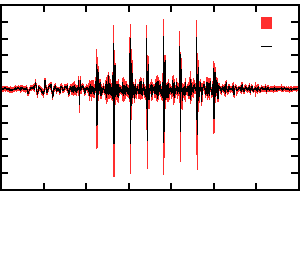
\includegraphics{voltage_0_108_gap_between_pulses_100_imaging_1st_av_with_sd_meansSub_large}}%
    \gplfronttext
  \end{picture}%
\endgroup
}\\
%  \quad
%   \subfloat[2nd pulse - 150]{
%     \label{fig:av:108:100_ex:second}
%     % GNUPLOT: LaTeX picture with Postscript
\begingroup
  \makeatletter
  \providecommand\color[2][]{%
    \GenericError{(gnuplot) \space\space\space\@spaces}{%
      Package color not loaded in conjunction with
      terminal option `colourtext'%
    }{See the gnuplot documentation for explanation.%
    }{Either use 'blacktext' in gnuplot or load the package
      color.sty in LaTeX.}%
    \renewcommand\color[2][]{}%
  }%
  \providecommand\includegraphics[2][]{%
    \GenericError{(gnuplot) \space\space\space\@spaces}{%
      Package graphicx or graphics not loaded%
    }{See the gnuplot documentation for explanation.%
    }{The gnuplot epslatex terminal needs graphicx.sty or graphics.sty.}%
    \renewcommand\includegraphics[2][]{}%
  }%
  \providecommand\rotatebox[2]{#2}%
  \@ifundefined{ifGPcolor}{%
    \newif\ifGPcolor
    \GPcolortrue
  }{}%
  \@ifundefined{ifGPblacktext}{%
    \newif\ifGPblacktext
    \GPblacktexttrue
  }{}%
  % define a \g@addto@macro without @ in the name:
  \let\gplgaddtomacro\g@addto@macro
  % define empty templates for all commands taking text:
  \gdef\gplbacktext{}%
  \gdef\gplfronttext{}%
  \makeatother
  \ifGPblacktext
    % no textcolor at all
    \def\colorrgb#1{}%
    \def\colorgray#1{}%
  \else
    % gray or color?
    \ifGPcolor
      \def\colorrgb#1{\color[rgb]{#1}}%
      \def\colorgray#1{\color[gray]{#1}}%
      \expandafter\def\csname LTw\endcsname{\color{white}}%
      \expandafter\def\csname LTb\endcsname{\color{black}}%
      \expandafter\def\csname LTa\endcsname{\color{black}}%
      \expandafter\def\csname LT0\endcsname{\color[rgb]{1,0,0}}%
      \expandafter\def\csname LT1\endcsname{\color[rgb]{0,1,0}}%
      \expandafter\def\csname LT2\endcsname{\color[rgb]{0,0,1}}%
      \expandafter\def\csname LT3\endcsname{\color[rgb]{1,0,1}}%
      \expandafter\def\csname LT4\endcsname{\color[rgb]{0,1,1}}%
      \expandafter\def\csname LT5\endcsname{\color[rgb]{1,1,0}}%
      \expandafter\def\csname LT6\endcsname{\color[rgb]{0,0,0}}%
      \expandafter\def\csname LT7\endcsname{\color[rgb]{1,0.3,0}}%
      \expandafter\def\csname LT8\endcsname{\color[rgb]{0.5,0.5,0.5}}%
    \else
      % gray
      \def\colorrgb#1{\color{black}}%
      \def\colorgray#1{\color[gray]{#1}}%
      \expandafter\def\csname LTw\endcsname{\color{white}}%
      \expandafter\def\csname LTb\endcsname{\color{black}}%
      \expandafter\def\csname LTa\endcsname{\color{black}}%
      \expandafter\def\csname LT0\endcsname{\color{black}}%
      \expandafter\def\csname LT1\endcsname{\color{black}}%
      \expandafter\def\csname LT2\endcsname{\color{black}}%
      \expandafter\def\csname LT3\endcsname{\color{black}}%
      \expandafter\def\csname LT4\endcsname{\color{black}}%
      \expandafter\def\csname LT5\endcsname{\color{black}}%
      \expandafter\def\csname LT6\endcsname{\color{black}}%
      \expandafter\def\csname LT7\endcsname{\color{black}}%
      \expandafter\def\csname LT8\endcsname{\color{black}}%
    \fi
  \fi
  \setlength{\unitlength}{0.0500bp}%
  \begin{picture}(2880.00,2520.00)%
    \gplgaddtomacro\gplbacktext{%
      \csname LTb\endcsname%
      \put(-119,704){\makebox(0,0)[r]{\strut{}-1.2}}%
      \put(-119,865){\makebox(0,0)[r]{\strut{}-1}}%
      \put(-119,1026){\makebox(0,0)[r]{\strut{}-0.8}}%
      \put(-119,1187){\makebox(0,0)[r]{\strut{}-0.6}}%
      \put(-119,1348){\makebox(0,0)[r]{\strut{}-0.4}}%
      \put(-119,1509){\makebox(0,0)[r]{\strut{}-0.2}}%
      \put(-119,1671){\makebox(0,0)[r]{\strut{} 0}}%
      \put(-119,1832){\makebox(0,0)[r]{\strut{} 0.2}}%
      \put(-119,1993){\makebox(0,0)[r]{\strut{} 0.4}}%
      \put(-119,2154){\makebox(0,0)[r]{\strut{} 0.6}}%
      \put(-119,2315){\makebox(0,0)[r]{\strut{} 0.8}}%
      \put(-119,2476){\makebox(0,0)[r]{\strut{} 1}}%
      \put(13,484){\makebox(0,0){\strut{} 0}}%
      \put(421,484){\makebox(0,0){\strut{} 5}}%
      \put(828,484){\makebox(0,0){\strut{} 10}}%
      \put(1236,484){\makebox(0,0){\strut{} 15}}%
      \put(1643,484){\makebox(0,0){\strut{} 20}}%
      \put(2051,484){\makebox(0,0){\strut{} 25}}%
      \put(2458,484){\makebox(0,0){\strut{} 30}}%
      \put(2866,484){\makebox(0,0){\strut{} 35}}%
      \put(-889,1590){\rotatebox{-270}{\makebox(0,0){\strut{}voltage (V)}}}%
      \put(1439,154){\makebox(0,0){\strut{}time ($\mu$ s)}}%
    }%
    \gplgaddtomacro\gplfronttext{%
      \csname LTb\endcsname%
      \put(2381,2303){\makebox(0,0)[r]{\strut{}1-$\sigma$}}%
      \csname LTb\endcsname%
      \put(2381,2083){\makebox(0,0)[r]{\strut{}av.}}%
    }%
    \gplbacktext
    \put(0,0){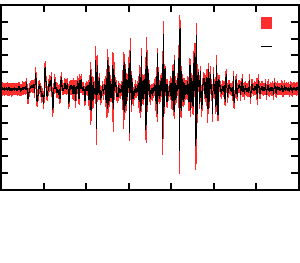
\includegraphics{voltage_0_108_gap_between_pulses_150_imaging_1st_av_with_sd_meansSub_large}}%
    \gplfronttext
  \end{picture}%
\endgroup
}\\
%  \quad
%   \subfloat[2nd pulse - 250]{
%     \label{fig:av:108:100_ex:second}
%     % GNUPLOT: LaTeX picture with Postscript
\begingroup
  \makeatletter
  \providecommand\color[2][]{%
    \GenericError{(gnuplot) \space\space\space\@spaces}{%
      Package color not loaded in conjunction with
      terminal option `colourtext'%
    }{See the gnuplot documentation for explanation.%
    }{Either use 'blacktext' in gnuplot or load the package
      color.sty in LaTeX.}%
    \renewcommand\color[2][]{}%
  }%
  \providecommand\includegraphics[2][]{%
    \GenericError{(gnuplot) \space\space\space\@spaces}{%
      Package graphicx or graphics not loaded%
    }{See the gnuplot documentation for explanation.%
    }{The gnuplot epslatex terminal needs graphicx.sty or graphics.sty.}%
    \renewcommand\includegraphics[2][]{}%
  }%
  \providecommand\rotatebox[2]{#2}%
  \@ifundefined{ifGPcolor}{%
    \newif\ifGPcolor
    \GPcolortrue
  }{}%
  \@ifundefined{ifGPblacktext}{%
    \newif\ifGPblacktext
    \GPblacktexttrue
  }{}%
  % define a \g@addto@macro without @ in the name:
  \let\gplgaddtomacro\g@addto@macro
  % define empty templates for all commands taking text:
  \gdef\gplbacktext{}%
  \gdef\gplfronttext{}%
  \makeatother
  \ifGPblacktext
    % no textcolor at all
    \def\colorrgb#1{}%
    \def\colorgray#1{}%
  \else
    % gray or color?
    \ifGPcolor
      \def\colorrgb#1{\color[rgb]{#1}}%
      \def\colorgray#1{\color[gray]{#1}}%
      \expandafter\def\csname LTw\endcsname{\color{white}}%
      \expandafter\def\csname LTb\endcsname{\color{black}}%
      \expandafter\def\csname LTa\endcsname{\color{black}}%
      \expandafter\def\csname LT0\endcsname{\color[rgb]{1,0,0}}%
      \expandafter\def\csname LT1\endcsname{\color[rgb]{0,1,0}}%
      \expandafter\def\csname LT2\endcsname{\color[rgb]{0,0,1}}%
      \expandafter\def\csname LT3\endcsname{\color[rgb]{1,0,1}}%
      \expandafter\def\csname LT4\endcsname{\color[rgb]{0,1,1}}%
      \expandafter\def\csname LT5\endcsname{\color[rgb]{1,1,0}}%
      \expandafter\def\csname LT6\endcsname{\color[rgb]{0,0,0}}%
      \expandafter\def\csname LT7\endcsname{\color[rgb]{1,0.3,0}}%
      \expandafter\def\csname LT8\endcsname{\color[rgb]{0.5,0.5,0.5}}%
    \else
      % gray
      \def\colorrgb#1{\color{black}}%
      \def\colorgray#1{\color[gray]{#1}}%
      \expandafter\def\csname LTw\endcsname{\color{white}}%
      \expandafter\def\csname LTb\endcsname{\color{black}}%
      \expandafter\def\csname LTa\endcsname{\color{black}}%
      \expandafter\def\csname LT0\endcsname{\color{black}}%
      \expandafter\def\csname LT1\endcsname{\color{black}}%
      \expandafter\def\csname LT2\endcsname{\color{black}}%
      \expandafter\def\csname LT3\endcsname{\color{black}}%
      \expandafter\def\csname LT4\endcsname{\color{black}}%
      \expandafter\def\csname LT5\endcsname{\color{black}}%
      \expandafter\def\csname LT6\endcsname{\color{black}}%
      \expandafter\def\csname LT7\endcsname{\color{black}}%
      \expandafter\def\csname LT8\endcsname{\color{black}}%
    \fi
  \fi
  \setlength{\unitlength}{0.0500bp}%
  \begin{picture}(2880.00,2520.00)%
    \gplgaddtomacro\gplbacktext{%
      \csname LTb\endcsname%
      \put(-119,704){\makebox(0,0)[r]{\strut{}-0.8}}%
      \put(-119,926){\makebox(0,0)[r]{\strut{}-0.6}}%
      \put(-119,1147){\makebox(0,0)[r]{\strut{}-0.4}}%
      \put(-119,1369){\makebox(0,0)[r]{\strut{}-0.2}}%
      \put(-119,1590){\makebox(0,0)[r]{\strut{} 0}}%
      \put(-119,1812){\makebox(0,0)[r]{\strut{} 0.2}}%
      \put(-119,2033){\makebox(0,0)[r]{\strut{} 0.4}}%
      \put(-119,2255){\makebox(0,0)[r]{\strut{} 0.6}}%
      \put(-119,2476){\makebox(0,0)[r]{\strut{} 0.8}}%
      \put(13,484){\makebox(0,0){\strut{} 0}}%
      \put(421,484){\makebox(0,0){\strut{} 5}}%
      \put(828,484){\makebox(0,0){\strut{} 10}}%
      \put(1236,484){\makebox(0,0){\strut{} 15}}%
      \put(1643,484){\makebox(0,0){\strut{} 20}}%
      \put(2051,484){\makebox(0,0){\strut{} 25}}%
      \put(2458,484){\makebox(0,0){\strut{} 30}}%
      \put(2866,484){\makebox(0,0){\strut{} 35}}%
      \put(-889,1590){\rotatebox{-270}{\makebox(0,0){\strut{}voltage (V)}}}%
      \put(1439,154){\makebox(0,0){\strut{}time ($\mu$ s)}}%
    }%
    \gplgaddtomacro\gplfronttext{%
      \csname LTb\endcsname%
      \put(2381,2303){\makebox(0,0)[r]{\strut{}1-$\sigma$}}%
      \csname LTb\endcsname%
      \put(2381,2083){\makebox(0,0)[r]{\strut{}av.}}%
    }%
    \gplbacktext
    \put(0,0){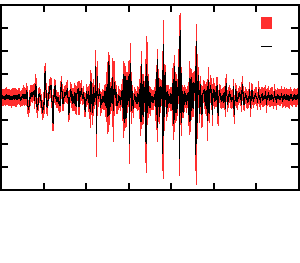
\includegraphics{voltage_0_108_gap_between_pulses_250_imaging_1st_av_with_sd_meansSub_large}}%
    \gplfronttext
  \end{picture}%
\endgroup
}
% \caption{
%     The pressure received  by the imaging transducer when the driving wave is on but the imaging wave is off (receive-only).
%     The second pulse \subref{fig:av:108:100:second} is received \unit{100}\micro\second\ after the first \subref{fig:av:108:100:first}.
%     Each image is the average of 49 images, the first standard-deviation error bars are indicated.
%   }
%   \label{fig:av:108:100_ex}
% \end{figure}

% \begin{figure}[t]%
%   \centering
%  %  \subfloat[1st pulse - 100]{
%  %    \label{fig:av:108:100_ex:first}
%  %    % GNUPLOT: LaTeX picture with Postscript
\begingroup
  \makeatletter
  \providecommand\color[2][]{%
    \GenericError{(gnuplot) \space\space\space\@spaces}{%
      Package color not loaded in conjunction with
      terminal option `colourtext'%
    }{See the gnuplot documentation for explanation.%
    }{Either use 'blacktext' in gnuplot or load the package
      color.sty in LaTeX.}%
    \renewcommand\color[2][]{}%
  }%
  \providecommand\includegraphics[2][]{%
    \GenericError{(gnuplot) \space\space\space\@spaces}{%
      Package graphicx or graphics not loaded%
    }{See the gnuplot documentation for explanation.%
    }{The gnuplot epslatex terminal needs graphicx.sty or graphics.sty.}%
    \renewcommand\includegraphics[2][]{}%
  }%
  \providecommand\rotatebox[2]{#2}%
  \@ifundefined{ifGPcolor}{%
    \newif\ifGPcolor
    \GPcolortrue
  }{}%
  \@ifundefined{ifGPblacktext}{%
    \newif\ifGPblacktext
    \GPblacktexttrue
  }{}%
  % define a \g@addto@macro without @ in the name:
  \let\gplgaddtomacro\g@addto@macro
  % define empty templates for all commands taking text:
  \gdef\gplbacktext{}%
  \gdef\gplfronttext{}%
  \makeatother
  \ifGPblacktext
    % no textcolor at all
    \def\colorrgb#1{}%
    \def\colorgray#1{}%
  \else
    % gray or color?
    \ifGPcolor
      \def\colorrgb#1{\color[rgb]{#1}}%
      \def\colorgray#1{\color[gray]{#1}}%
      \expandafter\def\csname LTw\endcsname{\color{white}}%
      \expandafter\def\csname LTb\endcsname{\color{black}}%
      \expandafter\def\csname LTa\endcsname{\color{black}}%
      \expandafter\def\csname LT0\endcsname{\color[rgb]{1,0,0}}%
      \expandafter\def\csname LT1\endcsname{\color[rgb]{0,1,0}}%
      \expandafter\def\csname LT2\endcsname{\color[rgb]{0,0,1}}%
      \expandafter\def\csname LT3\endcsname{\color[rgb]{1,0,1}}%
      \expandafter\def\csname LT4\endcsname{\color[rgb]{0,1,1}}%
      \expandafter\def\csname LT5\endcsname{\color[rgb]{1,1,0}}%
      \expandafter\def\csname LT6\endcsname{\color[rgb]{0,0,0}}%
      \expandafter\def\csname LT7\endcsname{\color[rgb]{1,0.3,0}}%
      \expandafter\def\csname LT8\endcsname{\color[rgb]{0.5,0.5,0.5}}%
    \else
      % gray
      \def\colorrgb#1{\color{black}}%
      \def\colorgray#1{\color[gray]{#1}}%
      \expandafter\def\csname LTw\endcsname{\color{white}}%
      \expandafter\def\csname LTb\endcsname{\color{black}}%
      \expandafter\def\csname LTa\endcsname{\color{black}}%
      \expandafter\def\csname LT0\endcsname{\color{black}}%
      \expandafter\def\csname LT1\endcsname{\color{black}}%
      \expandafter\def\csname LT2\endcsname{\color{black}}%
      \expandafter\def\csname LT3\endcsname{\color{black}}%
      \expandafter\def\csname LT4\endcsname{\color{black}}%
      \expandafter\def\csname LT5\endcsname{\color{black}}%
      \expandafter\def\csname LT6\endcsname{\color{black}}%
      \expandafter\def\csname LT7\endcsname{\color{black}}%
      \expandafter\def\csname LT8\endcsname{\color{black}}%
    \fi
  \fi
  \setlength{\unitlength}{0.0500bp}%
  \begin{picture}(2880.00,2520.00)%
    \gplgaddtomacro\gplbacktext{%
      \csname LTb\endcsname%
      \put(-119,704){\makebox(0,0)[r]{\strut{}-0.6}}%
      \put(-119,926){\makebox(0,0)[r]{\strut{}-0.4}}%
      \put(-119,1147){\makebox(0,0)[r]{\strut{}-0.2}}%
      \put(-119,1369){\makebox(0,0)[r]{\strut{} 0}}%
      \put(-119,1590){\makebox(0,0)[r]{\strut{} 0.2}}%
      \put(-119,1812){\makebox(0,0)[r]{\strut{} 0.4}}%
      \put(-119,2033){\makebox(0,0)[r]{\strut{} 0.6}}%
      \put(-119,2255){\makebox(0,0)[r]{\strut{} 0.8}}%
      \put(-119,2476){\makebox(0,0)[r]{\strut{} 1}}%
      \put(13,484){\makebox(0,0){\strut{} 17.5}}%
      \put(584,484){\makebox(0,0){\strut{} 18}}%
      \put(1154,484){\makebox(0,0){\strut{} 18.5}}%
      \put(1725,484){\makebox(0,0){\strut{} 19}}%
      \put(2295,484){\makebox(0,0){\strut{} 19.5}}%
      \put(2866,484){\makebox(0,0){\strut{} 20}}%
      \put(-889,1590){\rotatebox{-270}{\makebox(0,0){\strut{}voltage (V)}}}%
      \put(1439,154){\makebox(0,0){\strut{}time ($\mu$ s)}}%
    }%
    \gplgaddtomacro\gplfronttext{%
      \csname LTb\endcsname%
      \put(2381,2303){\makebox(0,0)[r]{\strut{}1-$\sigma$}}%
      \csname LTb\endcsname%
      \put(2381,2083){\makebox(0,0)[r]{\strut{}av.}}%
    }%
    \gplbacktext
    \put(0,0){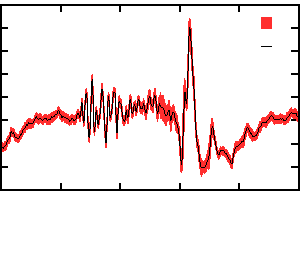
\includegraphics{voltage_0_108_gap_between_pulses_100_imaging_1st_av_with_sd_means1_large2}}%
    \gplfronttext
  \end{picture}%
\endgroup
}
%  % \quad
%  %  \subfloat[2nd pulse - 100]{
%  %    \label{fig:av:108:100_ex:second}
%  %    % GNUPLOT: LaTeX picture with Postscript
\begingroup
  \makeatletter
  \providecommand\color[2][]{%
    \GenericError{(gnuplot) \space\space\space\@spaces}{%
      Package color not loaded in conjunction with
      terminal option `colourtext'%
    }{See the gnuplot documentation for explanation.%
    }{Either use 'blacktext' in gnuplot or load the package
      color.sty in LaTeX.}%
    \renewcommand\color[2][]{}%
  }%
  \providecommand\includegraphics[2][]{%
    \GenericError{(gnuplot) \space\space\space\@spaces}{%
      Package graphicx or graphics not loaded%
    }{See the gnuplot documentation for explanation.%
    }{The gnuplot epslatex terminal needs graphicx.sty or graphics.sty.}%
    \renewcommand\includegraphics[2][]{}%
  }%
  \providecommand\rotatebox[2]{#2}%
  \@ifundefined{ifGPcolor}{%
    \newif\ifGPcolor
    \GPcolortrue
  }{}%
  \@ifundefined{ifGPblacktext}{%
    \newif\ifGPblacktext
    \GPblacktexttrue
  }{}%
  % define a \g@addto@macro without @ in the name:
  \let\gplgaddtomacro\g@addto@macro
  % define empty templates for all commands taking text:
  \gdef\gplbacktext{}%
  \gdef\gplfronttext{}%
  \makeatother
  \ifGPblacktext
    % no textcolor at all
    \def\colorrgb#1{}%
    \def\colorgray#1{}%
  \else
    % gray or color?
    \ifGPcolor
      \def\colorrgb#1{\color[rgb]{#1}}%
      \def\colorgray#1{\color[gray]{#1}}%
      \expandafter\def\csname LTw\endcsname{\color{white}}%
      \expandafter\def\csname LTb\endcsname{\color{black}}%
      \expandafter\def\csname LTa\endcsname{\color{black}}%
      \expandafter\def\csname LT0\endcsname{\color[rgb]{1,0,0}}%
      \expandafter\def\csname LT1\endcsname{\color[rgb]{0,1,0}}%
      \expandafter\def\csname LT2\endcsname{\color[rgb]{0,0,1}}%
      \expandafter\def\csname LT3\endcsname{\color[rgb]{1,0,1}}%
      \expandafter\def\csname LT4\endcsname{\color[rgb]{0,1,1}}%
      \expandafter\def\csname LT5\endcsname{\color[rgb]{1,1,0}}%
      \expandafter\def\csname LT6\endcsname{\color[rgb]{0,0,0}}%
      \expandafter\def\csname LT7\endcsname{\color[rgb]{1,0.3,0}}%
      \expandafter\def\csname LT8\endcsname{\color[rgb]{0.5,0.5,0.5}}%
    \else
      % gray
      \def\colorrgb#1{\color{black}}%
      \def\colorgray#1{\color[gray]{#1}}%
      \expandafter\def\csname LTw\endcsname{\color{white}}%
      \expandafter\def\csname LTb\endcsname{\color{black}}%
      \expandafter\def\csname LTa\endcsname{\color{black}}%
      \expandafter\def\csname LT0\endcsname{\color{black}}%
      \expandafter\def\csname LT1\endcsname{\color{black}}%
      \expandafter\def\csname LT2\endcsname{\color{black}}%
      \expandafter\def\csname LT3\endcsname{\color{black}}%
      \expandafter\def\csname LT4\endcsname{\color{black}}%
      \expandafter\def\csname LT5\endcsname{\color{black}}%
      \expandafter\def\csname LT6\endcsname{\color{black}}%
      \expandafter\def\csname LT7\endcsname{\color{black}}%
      \expandafter\def\csname LT8\endcsname{\color{black}}%
    \fi
  \fi
  \setlength{\unitlength}{0.0500bp}%
  \begin{picture}(2880.00,2520.00)%
    \gplgaddtomacro\gplbacktext{%
      \csname LTb\endcsname%
      \put(-119,704){\makebox(0,0)[r]{\strut{}}}%
      \put(-119,926){\makebox(0,0)[r]{\strut{}}}%
      \put(-119,1147){\makebox(0,0)[r]{\strut{}}}%
      \put(-119,1369){\makebox(0,0)[r]{\strut{}}}%
      \put(-119,1590){\makebox(0,0)[r]{\strut{}}}%
      \put(-119,1812){\makebox(0,0)[r]{\strut{}}}%
      \put(-119,2033){\makebox(0,0)[r]{\strut{}}}%
      \put(-119,2255){\makebox(0,0)[r]{\strut{}}}%
      \put(-119,2476){\makebox(0,0)[r]{\strut{}}}%
      \put(13,484){\makebox(0,0){\strut{} 17.5}}%
      \put(584,484){\makebox(0,0){\strut{} 18}}%
      \put(1154,484){\makebox(0,0){\strut{} 18.5}}%
      \put(1725,484){\makebox(0,0){\strut{} 19}}%
      \put(2295,484){\makebox(0,0){\strut{} 19.5}}%
      \put(2866,484){\makebox(0,0){\strut{} 20}}%
      \put(1439,154){\makebox(0,0){\strut{}time ($\mu$ s)}}%
    }%
    \gplgaddtomacro\gplfronttext{%
      \csname LTb\endcsname%
      \put(2381,2303){\makebox(0,0)[r]{\strut{}1-$\sigma$}}%
      \csname LTb\endcsname%
      \put(2381,2083){\makebox(0,0)[r]{\strut{}av.}}%
    }%
    \gplbacktext
    \put(0,0){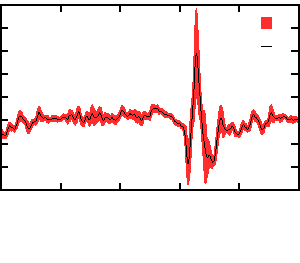
\includegraphics{voltage_0_108_gap_between_pulses_100_imaging_1st_av_with_sd_means2_large2}}%
    \gplfronttext
  \end{picture}%
\endgroup
}\\
%   \subfloat[1st pulse - 150]{
%     \label{fig:av:108:100_ex:first}
%     % GNUPLOT: LaTeX picture with Postscript
\begingroup
  \makeatletter
  \providecommand\color[2][]{%
    \GenericError{(gnuplot) \space\space\space\@spaces}{%
      Package color not loaded in conjunction with
      terminal option `colourtext'%
    }{See the gnuplot documentation for explanation.%
    }{Either use 'blacktext' in gnuplot or load the package
      color.sty in LaTeX.}%
    \renewcommand\color[2][]{}%
  }%
  \providecommand\includegraphics[2][]{%
    \GenericError{(gnuplot) \space\space\space\@spaces}{%
      Package graphicx or graphics not loaded%
    }{See the gnuplot documentation for explanation.%
    }{The gnuplot epslatex terminal needs graphicx.sty or graphics.sty.}%
    \renewcommand\includegraphics[2][]{}%
  }%
  \providecommand\rotatebox[2]{#2}%
  \@ifundefined{ifGPcolor}{%
    \newif\ifGPcolor
    \GPcolortrue
  }{}%
  \@ifundefined{ifGPblacktext}{%
    \newif\ifGPblacktext
    \GPblacktexttrue
  }{}%
  % define a \g@addto@macro without @ in the name:
  \let\gplgaddtomacro\g@addto@macro
  % define empty templates for all commands taking text:
  \gdef\gplbacktext{}%
  \gdef\gplfronttext{}%
  \makeatother
  \ifGPblacktext
    % no textcolor at all
    \def\colorrgb#1{}%
    \def\colorgray#1{}%
  \else
    % gray or color?
    \ifGPcolor
      \def\colorrgb#1{\color[rgb]{#1}}%
      \def\colorgray#1{\color[gray]{#1}}%
      \expandafter\def\csname LTw\endcsname{\color{white}}%
      \expandafter\def\csname LTb\endcsname{\color{black}}%
      \expandafter\def\csname LTa\endcsname{\color{black}}%
      \expandafter\def\csname LT0\endcsname{\color[rgb]{1,0,0}}%
      \expandafter\def\csname LT1\endcsname{\color[rgb]{0,1,0}}%
      \expandafter\def\csname LT2\endcsname{\color[rgb]{0,0,1}}%
      \expandafter\def\csname LT3\endcsname{\color[rgb]{1,0,1}}%
      \expandafter\def\csname LT4\endcsname{\color[rgb]{0,1,1}}%
      \expandafter\def\csname LT5\endcsname{\color[rgb]{1,1,0}}%
      \expandafter\def\csname LT6\endcsname{\color[rgb]{0,0,0}}%
      \expandafter\def\csname LT7\endcsname{\color[rgb]{1,0.3,0}}%
      \expandafter\def\csname LT8\endcsname{\color[rgb]{0.5,0.5,0.5}}%
    \else
      % gray
      \def\colorrgb#1{\color{black}}%
      \def\colorgray#1{\color[gray]{#1}}%
      \expandafter\def\csname LTw\endcsname{\color{white}}%
      \expandafter\def\csname LTb\endcsname{\color{black}}%
      \expandafter\def\csname LTa\endcsname{\color{black}}%
      \expandafter\def\csname LT0\endcsname{\color{black}}%
      \expandafter\def\csname LT1\endcsname{\color{black}}%
      \expandafter\def\csname LT2\endcsname{\color{black}}%
      \expandafter\def\csname LT3\endcsname{\color{black}}%
      \expandafter\def\csname LT4\endcsname{\color{black}}%
      \expandafter\def\csname LT5\endcsname{\color{black}}%
      \expandafter\def\csname LT6\endcsname{\color{black}}%
      \expandafter\def\csname LT7\endcsname{\color{black}}%
      \expandafter\def\csname LT8\endcsname{\color{black}}%
    \fi
  \fi
  \setlength{\unitlength}{0.0500bp}%
  \begin{picture}(2880.00,2520.00)%
    \gplgaddtomacro\gplbacktext{%
      \csname LTb\endcsname%
      \put(-119,704){\makebox(0,0)[r]{\strut{}-0.6}}%
      \put(-119,957){\makebox(0,0)[r]{\strut{}-0.4}}%
      \put(-119,1210){\makebox(0,0)[r]{\strut{}-0.2}}%
      \put(-119,1463){\makebox(0,0)[r]{\strut{} 0}}%
      \put(-119,1717){\makebox(0,0)[r]{\strut{} 0.2}}%
      \put(-119,1970){\makebox(0,0)[r]{\strut{} 0.4}}%
      \put(-119,2223){\makebox(0,0)[r]{\strut{} 0.6}}%
      \put(-119,2476){\makebox(0,0)[r]{\strut{} 0.8}}%
      \put(13,484){\makebox(0,0){\strut{} 17.5}}%
      \put(584,484){\makebox(0,0){\strut{} 18}}%
      \put(1154,484){\makebox(0,0){\strut{} 18.5}}%
      \put(1725,484){\makebox(0,0){\strut{} 19}}%
      \put(2295,484){\makebox(0,0){\strut{} 19.5}}%
      \put(2866,484){\makebox(0,0){\strut{} 20}}%
      \put(-889,1590){\rotatebox{-270}{\makebox(0,0){\strut{}}}}%
      \put(1439,154){\makebox(0,0){\strut{}time ($\mu$ s)}}%
    }%
    \gplgaddtomacro\gplfronttext{%
      \csname LTb\endcsname%
      \put(2381,2303){\makebox(0,0)[r]{\strut{}1-$\sigma$}}%
      \csname LTb\endcsname%
      \put(2381,2083){\makebox(0,0)[r]{\strut{}av.}}%
    }%
    \gplbacktext
    \put(0,0){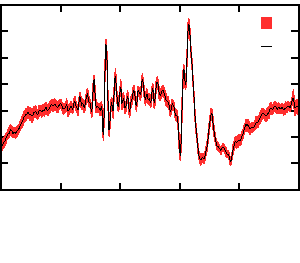
\includegraphics{voltage_0_108_gap_between_pulses_150_imaging_1st_av_with_sd_means1_large2}}%
    \gplfronttext
  \end{picture}%
\endgroup
}
%  \quad
%   \subfloat[2nd pulse - 150]{
%     \label{fig:av:108:100_ex:second}
%     % GNUPLOT: LaTeX picture with Postscript
\begingroup
  \makeatletter
  \providecommand\color[2][]{%
    \GenericError{(gnuplot) \space\space\space\@spaces}{%
      Package color not loaded in conjunction with
      terminal option `colourtext'%
    }{See the gnuplot documentation for explanation.%
    }{Either use 'blacktext' in gnuplot or load the package
      color.sty in LaTeX.}%
    \renewcommand\color[2][]{}%
  }%
  \providecommand\includegraphics[2][]{%
    \GenericError{(gnuplot) \space\space\space\@spaces}{%
      Package graphicx or graphics not loaded%
    }{See the gnuplot documentation for explanation.%
    }{The gnuplot epslatex terminal needs graphicx.sty or graphics.sty.}%
    \renewcommand\includegraphics[2][]{}%
  }%
  \providecommand\rotatebox[2]{#2}%
  \@ifundefined{ifGPcolor}{%
    \newif\ifGPcolor
    \GPcolortrue
  }{}%
  \@ifundefined{ifGPblacktext}{%
    \newif\ifGPblacktext
    \GPblacktexttrue
  }{}%
  % define a \g@addto@macro without @ in the name:
  \let\gplgaddtomacro\g@addto@macro
  % define empty templates for all commands taking text:
  \gdef\gplbacktext{}%
  \gdef\gplfronttext{}%
  \makeatother
  \ifGPblacktext
    % no textcolor at all
    \def\colorrgb#1{}%
    \def\colorgray#1{}%
  \else
    % gray or color?
    \ifGPcolor
      \def\colorrgb#1{\color[rgb]{#1}}%
      \def\colorgray#1{\color[gray]{#1}}%
      \expandafter\def\csname LTw\endcsname{\color{white}}%
      \expandafter\def\csname LTb\endcsname{\color{black}}%
      \expandafter\def\csname LTa\endcsname{\color{black}}%
      \expandafter\def\csname LT0\endcsname{\color[rgb]{1,0,0}}%
      \expandafter\def\csname LT1\endcsname{\color[rgb]{0,1,0}}%
      \expandafter\def\csname LT2\endcsname{\color[rgb]{0,0,1}}%
      \expandafter\def\csname LT3\endcsname{\color[rgb]{1,0,1}}%
      \expandafter\def\csname LT4\endcsname{\color[rgb]{0,1,1}}%
      \expandafter\def\csname LT5\endcsname{\color[rgb]{1,1,0}}%
      \expandafter\def\csname LT6\endcsname{\color[rgb]{0,0,0}}%
      \expandafter\def\csname LT7\endcsname{\color[rgb]{1,0.3,0}}%
      \expandafter\def\csname LT8\endcsname{\color[rgb]{0.5,0.5,0.5}}%
    \else
      % gray
      \def\colorrgb#1{\color{black}}%
      \def\colorgray#1{\color[gray]{#1}}%
      \expandafter\def\csname LTw\endcsname{\color{white}}%
      \expandafter\def\csname LTb\endcsname{\color{black}}%
      \expandafter\def\csname LTa\endcsname{\color{black}}%
      \expandafter\def\csname LT0\endcsname{\color{black}}%
      \expandafter\def\csname LT1\endcsname{\color{black}}%
      \expandafter\def\csname LT2\endcsname{\color{black}}%
      \expandafter\def\csname LT3\endcsname{\color{black}}%
      \expandafter\def\csname LT4\endcsname{\color{black}}%
      \expandafter\def\csname LT5\endcsname{\color{black}}%
      \expandafter\def\csname LT6\endcsname{\color{black}}%
      \expandafter\def\csname LT7\endcsname{\color{black}}%
      \expandafter\def\csname LT8\endcsname{\color{black}}%
    \fi
  \fi
  \setlength{\unitlength}{0.0500bp}%
  \begin{picture}(2880.00,2520.00)%
    \gplgaddtomacro\gplbacktext{%
      \csname LTb\endcsname%
      \put(-119,704){\makebox(0,0)[r]{\strut{}}}%
      \put(-119,926){\makebox(0,0)[r]{\strut{}}}%
      \put(-119,1147){\makebox(0,0)[r]{\strut{}}}%
      \put(-119,1369){\makebox(0,0)[r]{\strut{}}}%
      \put(-119,1590){\makebox(0,0)[r]{\strut{}}}%
      \put(-119,1812){\makebox(0,0)[r]{\strut{}}}%
      \put(-119,2033){\makebox(0,0)[r]{\strut{}}}%
      \put(-119,2255){\makebox(0,0)[r]{\strut{}}}%
      \put(-119,2476){\makebox(0,0)[r]{\strut{}}}%
      \put(13,484){\makebox(0,0){\strut{} 17.5}}%
      \put(584,484){\makebox(0,0){\strut{} 18}}%
      \put(1154,484){\makebox(0,0){\strut{} 18.5}}%
      \put(1725,484){\makebox(0,0){\strut{} 19}}%
      \put(2295,484){\makebox(0,0){\strut{} 19.5}}%
      \put(2866,484){\makebox(0,0){\strut{} 20}}%
      \put(1439,154){\makebox(0,0){\strut{}time ($\mu$ s)}}%
    }%
    \gplgaddtomacro\gplfronttext{%
      \csname LTb\endcsname%
      \put(2381,2303){\makebox(0,0)[r]{\strut{}1-$\sigma$}}%
      \csname LTb\endcsname%
      \put(2381,2083){\makebox(0,0)[r]{\strut{}av.}}%
    }%
    \gplbacktext
    \put(0,0){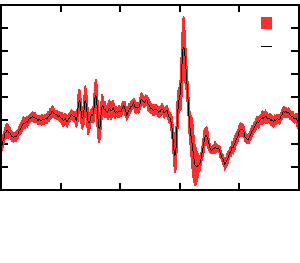
\includegraphics{voltage_0_108_gap_between_pulses_150_imaging_1st_av_with_sd_means2_large2}}%
    \gplfronttext
  \end{picture}%
\endgroup
}\\
%   \subfloat[1st pulse - 250]{
%     \label{fig:av:108:100_ex:first}
%     % GNUPLOT: LaTeX picture with Postscript
\begingroup
  \makeatletter
  \providecommand\color[2][]{%
    \GenericError{(gnuplot) \space\space\space\@spaces}{%
      Package color not loaded in conjunction with
      terminal option `colourtext'%
    }{See the gnuplot documentation for explanation.%
    }{Either use 'blacktext' in gnuplot or load the package
      color.sty in LaTeX.}%
    \renewcommand\color[2][]{}%
  }%
  \providecommand\includegraphics[2][]{%
    \GenericError{(gnuplot) \space\space\space\@spaces}{%
      Package graphicx or graphics not loaded%
    }{See the gnuplot documentation for explanation.%
    }{The gnuplot epslatex terminal needs graphicx.sty or graphics.sty.}%
    \renewcommand\includegraphics[2][]{}%
  }%
  \providecommand\rotatebox[2]{#2}%
  \@ifundefined{ifGPcolor}{%
    \newif\ifGPcolor
    \GPcolortrue
  }{}%
  \@ifundefined{ifGPblacktext}{%
    \newif\ifGPblacktext
    \GPblacktexttrue
  }{}%
  % define a \g@addto@macro without @ in the name:
  \let\gplgaddtomacro\g@addto@macro
  % define empty templates for all commands taking text:
  \gdef\gplbacktext{}%
  \gdef\gplfronttext{}%
  \makeatother
  \ifGPblacktext
    % no textcolor at all
    \def\colorrgb#1{}%
    \def\colorgray#1{}%
  \else
    % gray or color?
    \ifGPcolor
      \def\colorrgb#1{\color[rgb]{#1}}%
      \def\colorgray#1{\color[gray]{#1}}%
      \expandafter\def\csname LTw\endcsname{\color{white}}%
      \expandafter\def\csname LTb\endcsname{\color{black}}%
      \expandafter\def\csname LTa\endcsname{\color{black}}%
      \expandafter\def\csname LT0\endcsname{\color[rgb]{1,0,0}}%
      \expandafter\def\csname LT1\endcsname{\color[rgb]{0,1,0}}%
      \expandafter\def\csname LT2\endcsname{\color[rgb]{0,0,1}}%
      \expandafter\def\csname LT3\endcsname{\color[rgb]{1,0,1}}%
      \expandafter\def\csname LT4\endcsname{\color[rgb]{0,1,1}}%
      \expandafter\def\csname LT5\endcsname{\color[rgb]{1,1,0}}%
      \expandafter\def\csname LT6\endcsname{\color[rgb]{0,0,0}}%
      \expandafter\def\csname LT7\endcsname{\color[rgb]{1,0.3,0}}%
      \expandafter\def\csname LT8\endcsname{\color[rgb]{0.5,0.5,0.5}}%
    \else
      % gray
      \def\colorrgb#1{\color{black}}%
      \def\colorgray#1{\color[gray]{#1}}%
      \expandafter\def\csname LTw\endcsname{\color{white}}%
      \expandafter\def\csname LTb\endcsname{\color{black}}%
      \expandafter\def\csname LTa\endcsname{\color{black}}%
      \expandafter\def\csname LT0\endcsname{\color{black}}%
      \expandafter\def\csname LT1\endcsname{\color{black}}%
      \expandafter\def\csname LT2\endcsname{\color{black}}%
      \expandafter\def\csname LT3\endcsname{\color{black}}%
      \expandafter\def\csname LT4\endcsname{\color{black}}%
      \expandafter\def\csname LT5\endcsname{\color{black}}%
      \expandafter\def\csname LT6\endcsname{\color{black}}%
      \expandafter\def\csname LT7\endcsname{\color{black}}%
      \expandafter\def\csname LT8\endcsname{\color{black}}%
    \fi
  \fi
  \setlength{\unitlength}{0.0500bp}%
  \begin{picture}(2880.00,2520.00)%
    \gplgaddtomacro\gplbacktext{%
      \csname LTb\endcsname%
      \put(-119,704){\makebox(0,0)[r]{\strut{}-0.6}}%
      \put(-119,957){\makebox(0,0)[r]{\strut{}-0.4}}%
      \put(-119,1210){\makebox(0,0)[r]{\strut{}-0.2}}%
      \put(-119,1463){\makebox(0,0)[r]{\strut{} 0}}%
      \put(-119,1717){\makebox(0,0)[r]{\strut{} 0.2}}%
      \put(-119,1970){\makebox(0,0)[r]{\strut{} 0.4}}%
      \put(-119,2223){\makebox(0,0)[r]{\strut{} 0.6}}%
      \put(-119,2476){\makebox(0,0)[r]{\strut{} 0.8}}%
      \put(13,484){\makebox(0,0){\strut{} 17.5}}%
      \put(584,484){\makebox(0,0){\strut{} 18}}%
      \put(1154,484){\makebox(0,0){\strut{} 18.5}}%
      \put(1725,484){\makebox(0,0){\strut{} 19}}%
      \put(2295,484){\makebox(0,0){\strut{} 19.5}}%
      \put(2866,484){\makebox(0,0){\strut{} 20}}%
      \put(-889,1590){\rotatebox{-270}{\makebox(0,0){\strut{}voltage (V)}}}%
      \put(1439,154){\makebox(0,0){\strut{}time ($\mu$ s)}}%
    }%
    \gplgaddtomacro\gplfronttext{%
      \csname LTb\endcsname%
      \put(2381,2303){\makebox(0,0)[r]{\strut{}1-$\sigma$}}%
      \csname LTb\endcsname%
      \put(2381,2083){\makebox(0,0)[r]{\strut{}av.}}%
    }%
    \gplbacktext
    \put(0,0){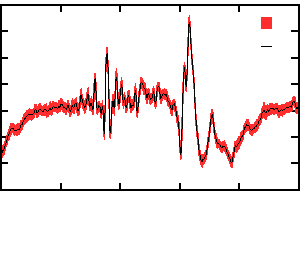
\includegraphics{voltage_0_108_gap_between_pulses_250_imaging_1st_av_with_sd_means1_large2}}%
    \gplfronttext
  \end{picture}%
\endgroup
}
%  \quad
%   \subfloat[2nd pulse - 250]{
%     \label{fig:av:108:100_ex:second}
%     % GNUPLOT: LaTeX picture with Postscript
\begingroup
  \makeatletter
  \providecommand\color[2][]{%
    \GenericError{(gnuplot) \space\space\space\@spaces}{%
      Package color not loaded in conjunction with
      terminal option `colourtext'%
    }{See the gnuplot documentation for explanation.%
    }{Either use 'blacktext' in gnuplot or load the package
      color.sty in LaTeX.}%
    \renewcommand\color[2][]{}%
  }%
  \providecommand\includegraphics[2][]{%
    \GenericError{(gnuplot) \space\space\space\@spaces}{%
      Package graphicx or graphics not loaded%
    }{See the gnuplot documentation for explanation.%
    }{The gnuplot epslatex terminal needs graphicx.sty or graphics.sty.}%
    \renewcommand\includegraphics[2][]{}%
  }%
  \providecommand\rotatebox[2]{#2}%
  \@ifundefined{ifGPcolor}{%
    \newif\ifGPcolor
    \GPcolortrue
  }{}%
  \@ifundefined{ifGPblacktext}{%
    \newif\ifGPblacktext
    \GPblacktexttrue
  }{}%
  % define a \g@addto@macro without @ in the name:
  \let\gplgaddtomacro\g@addto@macro
  % define empty templates for all commands taking text:
  \gdef\gplbacktext{}%
  \gdef\gplfronttext{}%
  \makeatother
  \ifGPblacktext
    % no textcolor at all
    \def\colorrgb#1{}%
    \def\colorgray#1{}%
  \else
    % gray or color?
    \ifGPcolor
      \def\colorrgb#1{\color[rgb]{#1}}%
      \def\colorgray#1{\color[gray]{#1}}%
      \expandafter\def\csname LTw\endcsname{\color{white}}%
      \expandafter\def\csname LTb\endcsname{\color{black}}%
      \expandafter\def\csname LTa\endcsname{\color{black}}%
      \expandafter\def\csname LT0\endcsname{\color[rgb]{1,0,0}}%
      \expandafter\def\csname LT1\endcsname{\color[rgb]{0,1,0}}%
      \expandafter\def\csname LT2\endcsname{\color[rgb]{0,0,1}}%
      \expandafter\def\csname LT3\endcsname{\color[rgb]{1,0,1}}%
      \expandafter\def\csname LT4\endcsname{\color[rgb]{0,1,1}}%
      \expandafter\def\csname LT5\endcsname{\color[rgb]{1,1,0}}%
      \expandafter\def\csname LT6\endcsname{\color[rgb]{0,0,0}}%
      \expandafter\def\csname LT7\endcsname{\color[rgb]{1,0.3,0}}%
      \expandafter\def\csname LT8\endcsname{\color[rgb]{0.5,0.5,0.5}}%
    \else
      % gray
      \def\colorrgb#1{\color{black}}%
      \def\colorgray#1{\color[gray]{#1}}%
      \expandafter\def\csname LTw\endcsname{\color{white}}%
      \expandafter\def\csname LTb\endcsname{\color{black}}%
      \expandafter\def\csname LTa\endcsname{\color{black}}%
      \expandafter\def\csname LT0\endcsname{\color{black}}%
      \expandafter\def\csname LT1\endcsname{\color{black}}%
      \expandafter\def\csname LT2\endcsname{\color{black}}%
      \expandafter\def\csname LT3\endcsname{\color{black}}%
      \expandafter\def\csname LT4\endcsname{\color{black}}%
      \expandafter\def\csname LT5\endcsname{\color{black}}%
      \expandafter\def\csname LT6\endcsname{\color{black}}%
      \expandafter\def\csname LT7\endcsname{\color{black}}%
      \expandafter\def\csname LT8\endcsname{\color{black}}%
    \fi
  \fi
  \setlength{\unitlength}{0.0500bp}%
  \begin{picture}(2880.00,2520.00)%
    \gplgaddtomacro\gplbacktext{%
      \csname LTb\endcsname%
      \put(-119,704){\makebox(0,0)[r]{\strut{}}}%
      \put(-119,926){\makebox(0,0)[r]{\strut{}}}%
      \put(-119,1147){\makebox(0,0)[r]{\strut{}}}%
      \put(-119,1369){\makebox(0,0)[r]{\strut{}}}%
      \put(-119,1590){\makebox(0,0)[r]{\strut{}}}%
      \put(-119,1812){\makebox(0,0)[r]{\strut{}}}%
      \put(-119,2033){\makebox(0,0)[r]{\strut{}}}%
      \put(-119,2255){\makebox(0,0)[r]{\strut{}}}%
      \put(-119,2476){\makebox(0,0)[r]{\strut{}}}%
      \put(13,484){\makebox(0,0){\strut{} 17.5}}%
      \put(584,484){\makebox(0,0){\strut{} 18}}%
      \put(1154,484){\makebox(0,0){\strut{} 18.5}}%
      \put(1725,484){\makebox(0,0){\strut{} 19}}%
      \put(2295,484){\makebox(0,0){\strut{} 19.5}}%
      \put(2866,484){\makebox(0,0){\strut{} 20}}%
      \put(1439,154){\makebox(0,0){\strut{}time ($\mu$ s)}}%
    }%
    \gplgaddtomacro\gplfronttext{%
      \csname LTb\endcsname%
      \put(2381,2303){\makebox(0,0)[r]{\strut{}1-$\sigma$}}%
      \csname LTb\endcsname%
      \put(2381,2083){\makebox(0,0)[r]{\strut{}av.}}%
    }%
    \gplbacktext
    \put(0,0){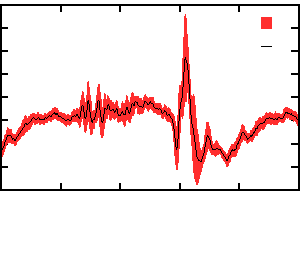
\includegraphics{voltage_0_108_gap_between_pulses_250_imaging_1st_av_with_sd_means2_large2}}%
    \gplfronttext
  \end{picture}%
\endgroup
}
% \caption{
%     The pressure received  by the imaging transducer when the driving wave is on but the imaging wave is off (receive-only).
%     The second pulse \subref{fig:av:108:100:second} is received \unit{100}\micro\second\ after the first \subref{fig:av:108:100:first}.
%     Each image is the average of 49 images, the first standard-deviation error bars are indicated.
%   }
%   \label{fig:av:108:100_ex}
% \end{figure}


% \begin{figure}[t]%
%   \centering
%  \quad
%   \subfloat[2nd pulse - 100 cross]{
%     \label{fig:av:108:100_ex:second}
%     % GNUPLOT: LaTeX picture with Postscript
\begingroup
  \makeatletter
  \providecommand\color[2][]{%
    \GenericError{(gnuplot) \space\space\space\@spaces}{%
      Package color not loaded in conjunction with
      terminal option `colourtext'%
    }{See the gnuplot documentation for explanation.%
    }{Either use 'blacktext' in gnuplot or load the package
      color.sty in LaTeX.}%
    \renewcommand\color[2][]{}%
  }%
  \providecommand\includegraphics[2][]{%
    \GenericError{(gnuplot) \space\space\space\@spaces}{%
      Package graphicx or graphics not loaded%
    }{See the gnuplot documentation for explanation.%
    }{The gnuplot epslatex terminal needs graphicx.sty or graphics.sty.}%
    \renewcommand\includegraphics[2][]{}%
  }%
  \providecommand\rotatebox[2]{#2}%
  \@ifundefined{ifGPcolor}{%
    \newif\ifGPcolor
    \GPcolortrue
  }{}%
  \@ifundefined{ifGPblacktext}{%
    \newif\ifGPblacktext
    \GPblacktexttrue
  }{}%
  % define a \g@addto@macro without @ in the name:
  \let\gplgaddtomacro\g@addto@macro
  % define empty templates for all commands taking text:
  \gdef\gplbacktext{}%
  \gdef\gplfronttext{}%
  \makeatother
  \ifGPblacktext
    % no textcolor at all
    \def\colorrgb#1{}%
    \def\colorgray#1{}%
  \else
    % gray or color?
    \ifGPcolor
      \def\colorrgb#1{\color[rgb]{#1}}%
      \def\colorgray#1{\color[gray]{#1}}%
      \expandafter\def\csname LTw\endcsname{\color{white}}%
      \expandafter\def\csname LTb\endcsname{\color{black}}%
      \expandafter\def\csname LTa\endcsname{\color{black}}%
      \expandafter\def\csname LT0\endcsname{\color[rgb]{1,0,0}}%
      \expandafter\def\csname LT1\endcsname{\color[rgb]{0,1,0}}%
      \expandafter\def\csname LT2\endcsname{\color[rgb]{0,0,1}}%
      \expandafter\def\csname LT3\endcsname{\color[rgb]{1,0,1}}%
      \expandafter\def\csname LT4\endcsname{\color[rgb]{0,1,1}}%
      \expandafter\def\csname LT5\endcsname{\color[rgb]{1,1,0}}%
      \expandafter\def\csname LT6\endcsname{\color[rgb]{0,0,0}}%
      \expandafter\def\csname LT7\endcsname{\color[rgb]{1,0.3,0}}%
      \expandafter\def\csname LT8\endcsname{\color[rgb]{0.5,0.5,0.5}}%
    \else
      % gray
      \def\colorrgb#1{\color{black}}%
      \def\colorgray#1{\color[gray]{#1}}%
      \expandafter\def\csname LTw\endcsname{\color{white}}%
      \expandafter\def\csname LTb\endcsname{\color{black}}%
      \expandafter\def\csname LTa\endcsname{\color{black}}%
      \expandafter\def\csname LT0\endcsname{\color{black}}%
      \expandafter\def\csname LT1\endcsname{\color{black}}%
      \expandafter\def\csname LT2\endcsname{\color{black}}%
      \expandafter\def\csname LT3\endcsname{\color{black}}%
      \expandafter\def\csname LT4\endcsname{\color{black}}%
      \expandafter\def\csname LT5\endcsname{\color{black}}%
      \expandafter\def\csname LT6\endcsname{\color{black}}%
      \expandafter\def\csname LT7\endcsname{\color{black}}%
      \expandafter\def\csname LT8\endcsname{\color{black}}%
    \fi
  \fi
  \setlength{\unitlength}{0.0500bp}%
  \begin{picture}(2880.00,2520.00)%
    \gplgaddtomacro\gplbacktext{%
      \csname LTb\endcsname%
      \put(-119,704){\makebox(0,0)[r]{\strut{}-1.5}}%
      \put(-119,957){\makebox(0,0)[r]{\strut{}-1}}%
      \put(-119,1210){\makebox(0,0)[r]{\strut{}-0.5}}%
      \put(-119,1463){\makebox(0,0)[r]{\strut{} 0}}%
      \put(-119,1717){\makebox(0,0)[r]{\strut{} 0.5}}%
      \put(-119,1970){\makebox(0,0)[r]{\strut{} 1}}%
      \put(-119,2223){\makebox(0,0)[r]{\strut{} 1.5}}%
      \put(-119,2476){\makebox(0,0)[r]{\strut{} 2}}%
      \put(13,484){\makebox(0,0){\strut{} 0}}%
      \put(421,484){\makebox(0,0){\strut{} 5}}%
      \put(828,484){\makebox(0,0){\strut{} 10}}%
      \put(1236,484){\makebox(0,0){\strut{} 15}}%
      \put(1643,484){\makebox(0,0){\strut{} 20}}%
      \put(2051,484){\makebox(0,0){\strut{} 25}}%
      \put(2458,484){\makebox(0,0){\strut{} 30}}%
      \put(2866,484){\makebox(0,0){\strut{} 35}}%
      \put(-889,1590){\rotatebox{-270}{\makebox(0,0){\strut{}voltage (V)}}}%
      \put(1439,154){\makebox(0,0){\strut{}time ($\mu$ s)}}%
    }%
    \gplgaddtomacro\gplfronttext{%
      \csname LTb\endcsname%
      \put(2381,2303){\makebox(0,0)[r]{\strut{}1-$\sigma$}}%
      \csname LTb\endcsname%
      \put(2381,2083){\makebox(0,0)[r]{\strut{}av.}}%
    }%
    \gplbacktext
    \put(0,0){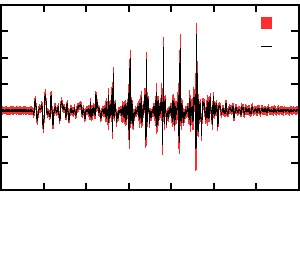
\includegraphics{voltage_0_108_gap_between_pulses_100_imaging_1st_av_with_sd_meansSub2_large_cross}}%
    \gplfronttext
  \end{picture}%
\endgroup
}\\
%  \quad
%   \subfloat[2nd pulse - 150]{
%     \label{fig:av:108:100_ex:second}
%     % GNUPLOT: LaTeX picture with Postscript
\begingroup
  \makeatletter
  \providecommand\color[2][]{%
    \GenericError{(gnuplot) \space\space\space\@spaces}{%
      Package color not loaded in conjunction with
      terminal option `colourtext'%
    }{See the gnuplot documentation for explanation.%
    }{Either use 'blacktext' in gnuplot or load the package
      color.sty in LaTeX.}%
    \renewcommand\color[2][]{}%
  }%
  \providecommand\includegraphics[2][]{%
    \GenericError{(gnuplot) \space\space\space\@spaces}{%
      Package graphicx or graphics not loaded%
    }{See the gnuplot documentation for explanation.%
    }{The gnuplot epslatex terminal needs graphicx.sty or graphics.sty.}%
    \renewcommand\includegraphics[2][]{}%
  }%
  \providecommand\rotatebox[2]{#2}%
  \@ifundefined{ifGPcolor}{%
    \newif\ifGPcolor
    \GPcolortrue
  }{}%
  \@ifundefined{ifGPblacktext}{%
    \newif\ifGPblacktext
    \GPblacktexttrue
  }{}%
  % define a \g@addto@macro without @ in the name:
  \let\gplgaddtomacro\g@addto@macro
  % define empty templates for all commands taking text:
  \gdef\gplbacktext{}%
  \gdef\gplfronttext{}%
  \makeatother
  \ifGPblacktext
    % no textcolor at all
    \def\colorrgb#1{}%
    \def\colorgray#1{}%
  \else
    % gray or color?
    \ifGPcolor
      \def\colorrgb#1{\color[rgb]{#1}}%
      \def\colorgray#1{\color[gray]{#1}}%
      \expandafter\def\csname LTw\endcsname{\color{white}}%
      \expandafter\def\csname LTb\endcsname{\color{black}}%
      \expandafter\def\csname LTa\endcsname{\color{black}}%
      \expandafter\def\csname LT0\endcsname{\color[rgb]{1,0,0}}%
      \expandafter\def\csname LT1\endcsname{\color[rgb]{0,1,0}}%
      \expandafter\def\csname LT2\endcsname{\color[rgb]{0,0,1}}%
      \expandafter\def\csname LT3\endcsname{\color[rgb]{1,0,1}}%
      \expandafter\def\csname LT4\endcsname{\color[rgb]{0,1,1}}%
      \expandafter\def\csname LT5\endcsname{\color[rgb]{1,1,0}}%
      \expandafter\def\csname LT6\endcsname{\color[rgb]{0,0,0}}%
      \expandafter\def\csname LT7\endcsname{\color[rgb]{1,0.3,0}}%
      \expandafter\def\csname LT8\endcsname{\color[rgb]{0.5,0.5,0.5}}%
    \else
      % gray
      \def\colorrgb#1{\color{black}}%
      \def\colorgray#1{\color[gray]{#1}}%
      \expandafter\def\csname LTw\endcsname{\color{white}}%
      \expandafter\def\csname LTb\endcsname{\color{black}}%
      \expandafter\def\csname LTa\endcsname{\color{black}}%
      \expandafter\def\csname LT0\endcsname{\color{black}}%
      \expandafter\def\csname LT1\endcsname{\color{black}}%
      \expandafter\def\csname LT2\endcsname{\color{black}}%
      \expandafter\def\csname LT3\endcsname{\color{black}}%
      \expandafter\def\csname LT4\endcsname{\color{black}}%
      \expandafter\def\csname LT5\endcsname{\color{black}}%
      \expandafter\def\csname LT6\endcsname{\color{black}}%
      \expandafter\def\csname LT7\endcsname{\color{black}}%
      \expandafter\def\csname LT8\endcsname{\color{black}}%
    \fi
  \fi
  \setlength{\unitlength}{0.0500bp}%
  \begin{picture}(2880.00,2520.00)%
    \gplgaddtomacro\gplbacktext{%
      \csname LTb\endcsname%
      \put(-119,704){\makebox(0,0)[r]{\strut{}-0.6}}%
      \put(-119,999){\makebox(0,0)[r]{\strut{}-0.4}}%
      \put(-119,1295){\makebox(0,0)[r]{\strut{}-0.2}}%
      \put(-119,1590){\makebox(0,0)[r]{\strut{} 0}}%
      \put(-119,1885){\makebox(0,0)[r]{\strut{} 0.2}}%
      \put(-119,2181){\makebox(0,0)[r]{\strut{} 0.4}}%
      \put(-119,2476){\makebox(0,0)[r]{\strut{} 0.6}}%
      \put(13,484){\makebox(0,0){\strut{} 0}}%
      \put(421,484){\makebox(0,0){\strut{} 5}}%
      \put(828,484){\makebox(0,0){\strut{} 10}}%
      \put(1236,484){\makebox(0,0){\strut{} 15}}%
      \put(1643,484){\makebox(0,0){\strut{} 20}}%
      \put(2051,484){\makebox(0,0){\strut{} 25}}%
      \put(2458,484){\makebox(0,0){\strut{} 30}}%
      \put(2866,484){\makebox(0,0){\strut{} 35}}%
      \put(-889,1590){\rotatebox{-270}{\makebox(0,0){\strut{}voltage (V)}}}%
      \put(1439,154){\makebox(0,0){\strut{}time ($\mu$ s)}}%
    }%
    \gplgaddtomacro\gplfronttext{%
      \csname LTb\endcsname%
      \put(2381,2303){\makebox(0,0)[r]{\strut{}1-$\sigma$}}%
      \csname LTb\endcsname%
      \put(2381,2083){\makebox(0,0)[r]{\strut{}av.}}%
    }%
    \gplbacktext
    \put(0,0){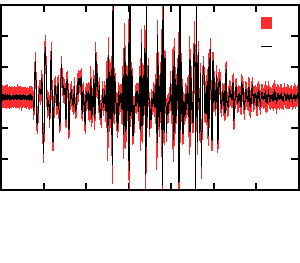
\includegraphics{voltage_0_108_gap_between_pulses_150_imaging_1st_av_with_sd_meansSub2_large_cross}}%
    \gplfronttext
  \end{picture}%
\endgroup
}\\
%  \quad
%   \subfloat[2nd pulse - 250]{
%     \label{fig:av:108:100_ex:second}
%     % GNUPLOT: LaTeX picture with Postscript
\begingroup
  \makeatletter
  \providecommand\color[2][]{%
    \GenericError{(gnuplot) \space\space\space\@spaces}{%
      Package color not loaded in conjunction with
      terminal option `colourtext'%
    }{See the gnuplot documentation for explanation.%
    }{Either use 'blacktext' in gnuplot or load the package
      color.sty in LaTeX.}%
    \renewcommand\color[2][]{}%
  }%
  \providecommand\includegraphics[2][]{%
    \GenericError{(gnuplot) \space\space\space\@spaces}{%
      Package graphicx or graphics not loaded%
    }{See the gnuplot documentation for explanation.%
    }{The gnuplot epslatex terminal needs graphicx.sty or graphics.sty.}%
    \renewcommand\includegraphics[2][]{}%
  }%
  \providecommand\rotatebox[2]{#2}%
  \@ifundefined{ifGPcolor}{%
    \newif\ifGPcolor
    \GPcolortrue
  }{}%
  \@ifundefined{ifGPblacktext}{%
    \newif\ifGPblacktext
    \GPblacktexttrue
  }{}%
  % define a \g@addto@macro without @ in the name:
  \let\gplgaddtomacro\g@addto@macro
  % define empty templates for all commands taking text:
  \gdef\gplbacktext{}%
  \gdef\gplfronttext{}%
  \makeatother
  \ifGPblacktext
    % no textcolor at all
    \def\colorrgb#1{}%
    \def\colorgray#1{}%
  \else
    % gray or color?
    \ifGPcolor
      \def\colorrgb#1{\color[rgb]{#1}}%
      \def\colorgray#1{\color[gray]{#1}}%
      \expandafter\def\csname LTw\endcsname{\color{white}}%
      \expandafter\def\csname LTb\endcsname{\color{black}}%
      \expandafter\def\csname LTa\endcsname{\color{black}}%
      \expandafter\def\csname LT0\endcsname{\color[rgb]{1,0,0}}%
      \expandafter\def\csname LT1\endcsname{\color[rgb]{0,1,0}}%
      \expandafter\def\csname LT2\endcsname{\color[rgb]{0,0,1}}%
      \expandafter\def\csname LT3\endcsname{\color[rgb]{1,0,1}}%
      \expandafter\def\csname LT4\endcsname{\color[rgb]{0,1,1}}%
      \expandafter\def\csname LT5\endcsname{\color[rgb]{1,1,0}}%
      \expandafter\def\csname LT6\endcsname{\color[rgb]{0,0,0}}%
      \expandafter\def\csname LT7\endcsname{\color[rgb]{1,0.3,0}}%
      \expandafter\def\csname LT8\endcsname{\color[rgb]{0.5,0.5,0.5}}%
    \else
      % gray
      \def\colorrgb#1{\color{black}}%
      \def\colorgray#1{\color[gray]{#1}}%
      \expandafter\def\csname LTw\endcsname{\color{white}}%
      \expandafter\def\csname LTb\endcsname{\color{black}}%
      \expandafter\def\csname LTa\endcsname{\color{black}}%
      \expandafter\def\csname LT0\endcsname{\color{black}}%
      \expandafter\def\csname LT1\endcsname{\color{black}}%
      \expandafter\def\csname LT2\endcsname{\color{black}}%
      \expandafter\def\csname LT3\endcsname{\color{black}}%
      \expandafter\def\csname LT4\endcsname{\color{black}}%
      \expandafter\def\csname LT5\endcsname{\color{black}}%
      \expandafter\def\csname LT6\endcsname{\color{black}}%
      \expandafter\def\csname LT7\endcsname{\color{black}}%
      \expandafter\def\csname LT8\endcsname{\color{black}}%
    \fi
  \fi
  \setlength{\unitlength}{0.0500bp}%
  \begin{picture}(2880.00,2520.00)%
    \gplgaddtomacro\gplbacktext{%
      \csname LTb\endcsname%
      \put(-119,704){\makebox(0,0)[r]{\strut{}-0.6}}%
      \put(-119,999){\makebox(0,0)[r]{\strut{}-0.4}}%
      \put(-119,1295){\makebox(0,0)[r]{\strut{}-0.2}}%
      \put(-119,1590){\makebox(0,0)[r]{\strut{} 0}}%
      \put(-119,1885){\makebox(0,0)[r]{\strut{} 0.2}}%
      \put(-119,2181){\makebox(0,0)[r]{\strut{} 0.4}}%
      \put(-119,2476){\makebox(0,0)[r]{\strut{} 0.6}}%
      \put(13,484){\makebox(0,0){\strut{} 0}}%
      \put(421,484){\makebox(0,0){\strut{} 5}}%
      \put(828,484){\makebox(0,0){\strut{} 10}}%
      \put(1236,484){\makebox(0,0){\strut{} 15}}%
      \put(1643,484){\makebox(0,0){\strut{} 20}}%
      \put(2051,484){\makebox(0,0){\strut{} 25}}%
      \put(2458,484){\makebox(0,0){\strut{} 30}}%
      \put(2866,484){\makebox(0,0){\strut{} 35}}%
      \put(-889,1590){\rotatebox{-270}{\makebox(0,0){\strut{}voltage (V)}}}%
      \put(1439,154){\makebox(0,0){\strut{}time ($\mu$ s)}}%
    }%
    \gplgaddtomacro\gplfronttext{%
      \csname LTb\endcsname%
      \put(2381,2303){\makebox(0,0)[r]{\strut{}1-$\sigma$}}%
      \csname LTb\endcsname%
      \put(2381,2083){\makebox(0,0)[r]{\strut{}av.}}%
    }%
    \gplbacktext
    \put(0,0){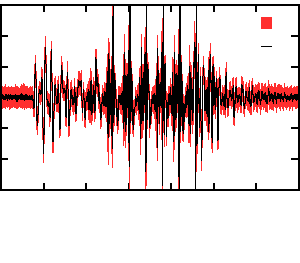
\includegraphics{voltage_0_108_gap_between_pulses_250_imaging_1st_av_with_sd_meansSub2_large_cross}}%
    \gplfronttext
  \end{picture}%
\endgroup
}
% \caption{
%     The pressure received  by the imaging transducer when the driving wave is on but the imaging wave is off (receive-only).
%     The second pulse \subref{fig:av:108:100:second} is received \unit{100}\micro\second\ after the first \subref{fig:av:108:100:first}.
%     Each image is the average of 49 images, the first standard-deviation error bars are indicated.
%   }
%   \label{fig:av:108:100_ex}
% \end{figure}

% \begin{figure}[t]%
%   \centering
%  \quad
%   \subfloat[2nd pulse - 100 cross]{
%     \label{fig:av:108:100_ex:second}
%     % GNUPLOT: LaTeX picture with Postscript
\begingroup
  \makeatletter
  \providecommand\color[2][]{%
    \GenericError{(gnuplot) \space\space\space\@spaces}{%
      Package color not loaded in conjunction with
      terminal option `colourtext'%
    }{See the gnuplot documentation for explanation.%
    }{Either use 'blacktext' in gnuplot or load the package
      color.sty in LaTeX.}%
    \renewcommand\color[2][]{}%
  }%
  \providecommand\includegraphics[2][]{%
    \GenericError{(gnuplot) \space\space\space\@spaces}{%
      Package graphicx or graphics not loaded%
    }{See the gnuplot documentation for explanation.%
    }{The gnuplot epslatex terminal needs graphicx.sty or graphics.sty.}%
    \renewcommand\includegraphics[2][]{}%
  }%
  \providecommand\rotatebox[2]{#2}%
  \@ifundefined{ifGPcolor}{%
    \newif\ifGPcolor
    \GPcolortrue
  }{}%
  \@ifundefined{ifGPblacktext}{%
    \newif\ifGPblacktext
    \GPblacktexttrue
  }{}%
  % define a \g@addto@macro without @ in the name:
  \let\gplgaddtomacro\g@addto@macro
  % define empty templates for all commands taking text:
  \gdef\gplbacktext{}%
  \gdef\gplfronttext{}%
  \makeatother
  \ifGPblacktext
    % no textcolor at all
    \def\colorrgb#1{}%
    \def\colorgray#1{}%
  \else
    % gray or color?
    \ifGPcolor
      \def\colorrgb#1{\color[rgb]{#1}}%
      \def\colorgray#1{\color[gray]{#1}}%
      \expandafter\def\csname LTw\endcsname{\color{white}}%
      \expandafter\def\csname LTb\endcsname{\color{black}}%
      \expandafter\def\csname LTa\endcsname{\color{black}}%
      \expandafter\def\csname LT0\endcsname{\color[rgb]{1,0,0}}%
      \expandafter\def\csname LT1\endcsname{\color[rgb]{0,1,0}}%
      \expandafter\def\csname LT2\endcsname{\color[rgb]{0,0,1}}%
      \expandafter\def\csname LT3\endcsname{\color[rgb]{1,0,1}}%
      \expandafter\def\csname LT4\endcsname{\color[rgb]{0,1,1}}%
      \expandafter\def\csname LT5\endcsname{\color[rgb]{1,1,0}}%
      \expandafter\def\csname LT6\endcsname{\color[rgb]{0,0,0}}%
      \expandafter\def\csname LT7\endcsname{\color[rgb]{1,0.3,0}}%
      \expandafter\def\csname LT8\endcsname{\color[rgb]{0.5,0.5,0.5}}%
    \else
      % gray
      \def\colorrgb#1{\color{black}}%
      \def\colorgray#1{\color[gray]{#1}}%
      \expandafter\def\csname LTw\endcsname{\color{white}}%
      \expandafter\def\csname LTb\endcsname{\color{black}}%
      \expandafter\def\csname LTa\endcsname{\color{black}}%
      \expandafter\def\csname LT0\endcsname{\color{black}}%
      \expandafter\def\csname LT1\endcsname{\color{black}}%
      \expandafter\def\csname LT2\endcsname{\color{black}}%
      \expandafter\def\csname LT3\endcsname{\color{black}}%
      \expandafter\def\csname LT4\endcsname{\color{black}}%
      \expandafter\def\csname LT5\endcsname{\color{black}}%
      \expandafter\def\csname LT6\endcsname{\color{black}}%
      \expandafter\def\csname LT7\endcsname{\color{black}}%
      \expandafter\def\csname LT8\endcsname{\color{black}}%
    \fi
  \fi
  \setlength{\unitlength}{0.0500bp}%
  \begin{picture}(2880.00,2520.00)%
    \gplgaddtomacro\gplbacktext{%
      \csname LTb\endcsname%
      \put(-119,704){\makebox(0,0)[r]{\strut{}-1}}%
      \put(-119,1058){\makebox(0,0)[r]{\strut{}-0.5}}%
      \put(-119,1413){\makebox(0,0)[r]{\strut{} 0}}%
      \put(-119,1767){\makebox(0,0)[r]{\strut{} 0.5}}%
      \put(-119,2122){\makebox(0,0)[r]{\strut{} 1}}%
      \put(-119,2476){\makebox(0,0)[r]{\strut{} 1.5}}%
      \put(13,484){\makebox(0,0){\strut{} 17.5}}%
      \put(584,484){\makebox(0,0){\strut{} 18}}%
      \put(1154,484){\makebox(0,0){\strut{} 18.5}}%
      \put(1725,484){\makebox(0,0){\strut{} 19}}%
      \put(2295,484){\makebox(0,0){\strut{} 19.5}}%
      \put(2866,484){\makebox(0,0){\strut{} 20}}%
      \put(-889,1590){\rotatebox{-270}{\makebox(0,0){\strut{}voltage (V)}}}%
      \put(1439,154){\makebox(0,0){\strut{}time ($\mu$ s)}}%
    }%
    \gplgaddtomacro\gplfronttext{%
      \csname LTb\endcsname%
      \put(2381,2303){\makebox(0,0)[r]{\strut{}1-$\sigma$}}%
      \csname LTb\endcsname%
      \put(2381,2083){\makebox(0,0)[r]{\strut{}av.}}%
    }%
    \gplbacktext
    \put(0,0){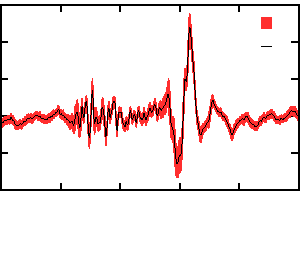
\includegraphics{voltage_0_108_gap_between_pulses_100_imaging_1st_av_with_sd_meansSub2_large2_cross}}%
    \gplfronttext
  \end{picture}%
\endgroup
}\\
%  \quad
%   \subfloat[2nd pulse - 150]{
%     \label{fig:av:108:100_ex:second}
%     % GNUPLOT: LaTeX picture with Postscript
\begingroup
  \makeatletter
  \providecommand\color[2][]{%
    \GenericError{(gnuplot) \space\space\space\@spaces}{%
      Package color not loaded in conjunction with
      terminal option `colourtext'%
    }{See the gnuplot documentation for explanation.%
    }{Either use 'blacktext' in gnuplot or load the package
      color.sty in LaTeX.}%
    \renewcommand\color[2][]{}%
  }%
  \providecommand\includegraphics[2][]{%
    \GenericError{(gnuplot) \space\space\space\@spaces}{%
      Package graphicx or graphics not loaded%
    }{See the gnuplot documentation for explanation.%
    }{The gnuplot epslatex terminal needs graphicx.sty or graphics.sty.}%
    \renewcommand\includegraphics[2][]{}%
  }%
  \providecommand\rotatebox[2]{#2}%
  \@ifundefined{ifGPcolor}{%
    \newif\ifGPcolor
    \GPcolortrue
  }{}%
  \@ifundefined{ifGPblacktext}{%
    \newif\ifGPblacktext
    \GPblacktexttrue
  }{}%
  % define a \g@addto@macro without @ in the name:
  \let\gplgaddtomacro\g@addto@macro
  % define empty templates for all commands taking text:
  \gdef\gplbacktext{}%
  \gdef\gplfronttext{}%
  \makeatother
  \ifGPblacktext
    % no textcolor at all
    \def\colorrgb#1{}%
    \def\colorgray#1{}%
  \else
    % gray or color?
    \ifGPcolor
      \def\colorrgb#1{\color[rgb]{#1}}%
      \def\colorgray#1{\color[gray]{#1}}%
      \expandafter\def\csname LTw\endcsname{\color{white}}%
      \expandafter\def\csname LTb\endcsname{\color{black}}%
      \expandafter\def\csname LTa\endcsname{\color{black}}%
      \expandafter\def\csname LT0\endcsname{\color[rgb]{1,0,0}}%
      \expandafter\def\csname LT1\endcsname{\color[rgb]{0,1,0}}%
      \expandafter\def\csname LT2\endcsname{\color[rgb]{0,0,1}}%
      \expandafter\def\csname LT3\endcsname{\color[rgb]{1,0,1}}%
      \expandafter\def\csname LT4\endcsname{\color[rgb]{0,1,1}}%
      \expandafter\def\csname LT5\endcsname{\color[rgb]{1,1,0}}%
      \expandafter\def\csname LT6\endcsname{\color[rgb]{0,0,0}}%
      \expandafter\def\csname LT7\endcsname{\color[rgb]{1,0.3,0}}%
      \expandafter\def\csname LT8\endcsname{\color[rgb]{0.5,0.5,0.5}}%
    \else
      % gray
      \def\colorrgb#1{\color{black}}%
      \def\colorgray#1{\color[gray]{#1}}%
      \expandafter\def\csname LTw\endcsname{\color{white}}%
      \expandafter\def\csname LTb\endcsname{\color{black}}%
      \expandafter\def\csname LTa\endcsname{\color{black}}%
      \expandafter\def\csname LT0\endcsname{\color{black}}%
      \expandafter\def\csname LT1\endcsname{\color{black}}%
      \expandafter\def\csname LT2\endcsname{\color{black}}%
      \expandafter\def\csname LT3\endcsname{\color{black}}%
      \expandafter\def\csname LT4\endcsname{\color{black}}%
      \expandafter\def\csname LT5\endcsname{\color{black}}%
      \expandafter\def\csname LT6\endcsname{\color{black}}%
      \expandafter\def\csname LT7\endcsname{\color{black}}%
      \expandafter\def\csname LT8\endcsname{\color{black}}%
    \fi
  \fi
  \setlength{\unitlength}{0.0500bp}%
  \begin{picture}(2880.00,2520.00)%
    \gplgaddtomacro\gplbacktext{%
      \csname LTb\endcsname%
      \put(-119,704){\makebox(0,0)[r]{\strut{}-0.6}}%
      \put(-119,999){\makebox(0,0)[r]{\strut{}-0.4}}%
      \put(-119,1295){\makebox(0,0)[r]{\strut{}-0.2}}%
      \put(-119,1590){\makebox(0,0)[r]{\strut{} 0}}%
      \put(-119,1885){\makebox(0,0)[r]{\strut{} 0.2}}%
      \put(-119,2181){\makebox(0,0)[r]{\strut{} 0.4}}%
      \put(-119,2476){\makebox(0,0)[r]{\strut{} 0.6}}%
      \put(13,484){\makebox(0,0){\strut{} 17.5}}%
      \put(584,484){\makebox(0,0){\strut{} 18}}%
      \put(1154,484){\makebox(0,0){\strut{} 18.5}}%
      \put(1725,484){\makebox(0,0){\strut{} 19}}%
      \put(2295,484){\makebox(0,0){\strut{} 19.5}}%
      \put(2866,484){\makebox(0,0){\strut{} 20}}%
      \put(1439,154){\makebox(0,0){\strut{}time ($\mu$ s)}}%
    }%
    \gplgaddtomacro\gplfronttext{%
      \csname LTb\endcsname%
      \put(2381,2303){\makebox(0,0)[r]{\strut{}1-$\sigma$}}%
      \csname LTb\endcsname%
      \put(2381,2083){\makebox(0,0)[r]{\strut{}av.}}%
    }%
    \gplbacktext
    \put(0,0){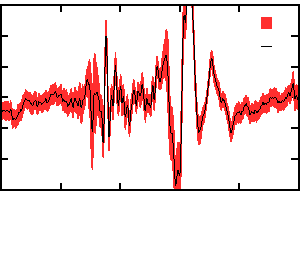
\includegraphics{voltage_0_108_gap_between_pulses_150_imaging_1st_av_with_sd_meansSub2_large2_cross}}%
    \gplfronttext
  \end{picture}%
\endgroup
}\\
%  \quad
%   \subfloat[2nd pulse - 250]{
%     \label{fig:av:108:100_ex:second}
%     % GNUPLOT: LaTeX picture with Postscript
\begingroup
  \makeatletter
  \providecommand\color[2][]{%
    \GenericError{(gnuplot) \space\space\space\@spaces}{%
      Package color not loaded in conjunction with
      terminal option `colourtext'%
    }{See the gnuplot documentation for explanation.%
    }{Either use 'blacktext' in gnuplot or load the package
      color.sty in LaTeX.}%
    \renewcommand\color[2][]{}%
  }%
  \providecommand\includegraphics[2][]{%
    \GenericError{(gnuplot) \space\space\space\@spaces}{%
      Package graphicx or graphics not loaded%
    }{See the gnuplot documentation for explanation.%
    }{The gnuplot epslatex terminal needs graphicx.sty or graphics.sty.}%
    \renewcommand\includegraphics[2][]{}%
  }%
  \providecommand\rotatebox[2]{#2}%
  \@ifundefined{ifGPcolor}{%
    \newif\ifGPcolor
    \GPcolortrue
  }{}%
  \@ifundefined{ifGPblacktext}{%
    \newif\ifGPblacktext
    \GPblacktexttrue
  }{}%
  % define a \g@addto@macro without @ in the name:
  \let\gplgaddtomacro\g@addto@macro
  % define empty templates for all commands taking text:
  \gdef\gplbacktext{}%
  \gdef\gplfronttext{}%
  \makeatother
  \ifGPblacktext
    % no textcolor at all
    \def\colorrgb#1{}%
    \def\colorgray#1{}%
  \else
    % gray or color?
    \ifGPcolor
      \def\colorrgb#1{\color[rgb]{#1}}%
      \def\colorgray#1{\color[gray]{#1}}%
      \expandafter\def\csname LTw\endcsname{\color{white}}%
      \expandafter\def\csname LTb\endcsname{\color{black}}%
      \expandafter\def\csname LTa\endcsname{\color{black}}%
      \expandafter\def\csname LT0\endcsname{\color[rgb]{1,0,0}}%
      \expandafter\def\csname LT1\endcsname{\color[rgb]{0,1,0}}%
      \expandafter\def\csname LT2\endcsname{\color[rgb]{0,0,1}}%
      \expandafter\def\csname LT3\endcsname{\color[rgb]{1,0,1}}%
      \expandafter\def\csname LT4\endcsname{\color[rgb]{0,1,1}}%
      \expandafter\def\csname LT5\endcsname{\color[rgb]{1,1,0}}%
      \expandafter\def\csname LT6\endcsname{\color[rgb]{0,0,0}}%
      \expandafter\def\csname LT7\endcsname{\color[rgb]{1,0.3,0}}%
      \expandafter\def\csname LT8\endcsname{\color[rgb]{0.5,0.5,0.5}}%
    \else
      % gray
      \def\colorrgb#1{\color{black}}%
      \def\colorgray#1{\color[gray]{#1}}%
      \expandafter\def\csname LTw\endcsname{\color{white}}%
      \expandafter\def\csname LTb\endcsname{\color{black}}%
      \expandafter\def\csname LTa\endcsname{\color{black}}%
      \expandafter\def\csname LT0\endcsname{\color{black}}%
      \expandafter\def\csname LT1\endcsname{\color{black}}%
      \expandafter\def\csname LT2\endcsname{\color{black}}%
      \expandafter\def\csname LT3\endcsname{\color{black}}%
      \expandafter\def\csname LT4\endcsname{\color{black}}%
      \expandafter\def\csname LT5\endcsname{\color{black}}%
      \expandafter\def\csname LT6\endcsname{\color{black}}%
      \expandafter\def\csname LT7\endcsname{\color{black}}%
      \expandafter\def\csname LT8\endcsname{\color{black}}%
    \fi
  \fi
  \setlength{\unitlength}{0.0500bp}%
  \begin{picture}(2880.00,2520.00)%
    \gplgaddtomacro\gplbacktext{%
      \csname LTb\endcsname%
      \put(-119,704){\makebox(0,0)[r]{\strut{}-0.6}}%
      \put(-119,999){\makebox(0,0)[r]{\strut{}-0.4}}%
      \put(-119,1295){\makebox(0,0)[r]{\strut{}-0.2}}%
      \put(-119,1590){\makebox(0,0)[r]{\strut{} 0}}%
      \put(-119,1885){\makebox(0,0)[r]{\strut{} 0.2}}%
      \put(-119,2181){\makebox(0,0)[r]{\strut{} 0.4}}%
      \put(-119,2476){\makebox(0,0)[r]{\strut{} 0.6}}%
      \put(13,484){\makebox(0,0){\strut{} 17.5}}%
      \put(584,484){\makebox(0,0){\strut{} 18}}%
      \put(1154,484){\makebox(0,0){\strut{} 18.5}}%
      \put(1725,484){\makebox(0,0){\strut{} 19}}%
      \put(2295,484){\makebox(0,0){\strut{} 19.5}}%
      \put(2866,484){\makebox(0,0){\strut{} 20}}%
      \put(1439,154){\makebox(0,0){\strut{}time ($\mu$ s)}}%
    }%
    \gplgaddtomacro\gplfronttext{%
      \csname LTb\endcsname%
      \put(2381,2303){\makebox(0,0)[r]{\strut{}1-$\sigma$}}%
      \csname LTb\endcsname%
      \put(2381,2083){\makebox(0,0)[r]{\strut{}av.}}%
    }%
    \gplbacktext
    \put(0,0){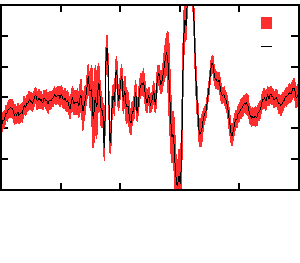
\includegraphics{voltage_0_108_gap_between_pulses_250_imaging_1st_av_with_sd_meansSub2_large2_cross}}%
    \gplfronttext
  \end{picture}%
\endgroup
}
% \caption{
%     The pressure received  by the imaging transducer when the driving wave is on but the imaging wave is off (receive-only).
%     The second pulse \subref{fig:av:108:100:second} is received \unit{100}\micro\second\ after the first \subref{fig:av:108:100:first}.
%     Each image is the average of 49 images, the first standard-deviation error bars are indicated.
%   }
%   \label{fig:av:108:100_ex}
% \end{figure}

\subsection{Pulse-echo imaging of the first driving pulse}



\begin{figure}[t]%
  \centering
 % \quad
 %  \subfloat[1st pulse - 100]{
 %    \label{fig:av:108:100_ex:first}
 %    % GNUPLOT: LaTeX picture with Postscript
\begingroup
  \makeatletter
  \providecommand\color[2][]{%
    \GenericError{(gnuplot) \space\space\space\@spaces}{%
      Package color not loaded in conjunction with
      terminal option `colourtext'%
    }{See the gnuplot documentation for explanation.%
    }{Either use 'blacktext' in gnuplot or load the package
      color.sty in LaTeX.}%
    \renewcommand\color[2][]{}%
  }%
  \providecommand\includegraphics[2][]{%
    \GenericError{(gnuplot) \space\space\space\@spaces}{%
      Package graphicx or graphics not loaded%
    }{See the gnuplot documentation for explanation.%
    }{The gnuplot epslatex terminal needs graphicx.sty or graphics.sty.}%
    \renewcommand\includegraphics[2][]{}%
  }%
  \providecommand\rotatebox[2]{#2}%
  \@ifundefined{ifGPcolor}{%
    \newif\ifGPcolor
    \GPcolortrue
  }{}%
  \@ifundefined{ifGPblacktext}{%
    \newif\ifGPblacktext
    \GPblacktexttrue
  }{}%
  % define a \g@addto@macro without @ in the name:
  \let\gplgaddtomacro\g@addto@macro
  % define empty templates for all commands taking text:
  \gdef\gplbacktext{}%
  \gdef\gplfronttext{}%
  \makeatother
  \ifGPblacktext
    % no textcolor at all
    \def\colorrgb#1{}%
    \def\colorgray#1{}%
  \else
    % gray or color?
    \ifGPcolor
      \def\colorrgb#1{\color[rgb]{#1}}%
      \def\colorgray#1{\color[gray]{#1}}%
      \expandafter\def\csname LTw\endcsname{\color{white}}%
      \expandafter\def\csname LTb\endcsname{\color{black}}%
      \expandafter\def\csname LTa\endcsname{\color{black}}%
      \expandafter\def\csname LT0\endcsname{\color[rgb]{1,0,0}}%
      \expandafter\def\csname LT1\endcsname{\color[rgb]{0,1,0}}%
      \expandafter\def\csname LT2\endcsname{\color[rgb]{0,0,1}}%
      \expandafter\def\csname LT3\endcsname{\color[rgb]{1,0,1}}%
      \expandafter\def\csname LT4\endcsname{\color[rgb]{0,1,1}}%
      \expandafter\def\csname LT5\endcsname{\color[rgb]{1,1,0}}%
      \expandafter\def\csname LT6\endcsname{\color[rgb]{0,0,0}}%
      \expandafter\def\csname LT7\endcsname{\color[rgb]{1,0.3,0}}%
      \expandafter\def\csname LT8\endcsname{\color[rgb]{0.5,0.5,0.5}}%
    \else
      % gray
      \def\colorrgb#1{\color{black}}%
      \def\colorgray#1{\color[gray]{#1}}%
      \expandafter\def\csname LTw\endcsname{\color{white}}%
      \expandafter\def\csname LTb\endcsname{\color{black}}%
      \expandafter\def\csname LTa\endcsname{\color{black}}%
      \expandafter\def\csname LT0\endcsname{\color{black}}%
      \expandafter\def\csname LT1\endcsname{\color{black}}%
      \expandafter\def\csname LT2\endcsname{\color{black}}%
      \expandafter\def\csname LT3\endcsname{\color{black}}%
      \expandafter\def\csname LT4\endcsname{\color{black}}%
      \expandafter\def\csname LT5\endcsname{\color{black}}%
      \expandafter\def\csname LT6\endcsname{\color{black}}%
      \expandafter\def\csname LT7\endcsname{\color{black}}%
      \expandafter\def\csname LT8\endcsname{\color{black}}%
    \fi
  \fi
  \setlength{\unitlength}{0.0500bp}%
  \begin{picture}(2880.00,2520.00)%
    \gplgaddtomacro\gplbacktext{%
      \csname LTb\endcsname%
      \put(-119,704){\makebox(0,0)[r]{\strut{}-0.6}}%
      \put(-119,957){\makebox(0,0)[r]{\strut{}-0.4}}%
      \put(-119,1210){\makebox(0,0)[r]{\strut{}-0.2}}%
      \put(-119,1463){\makebox(0,0)[r]{\strut{} 0}}%
      \put(-119,1717){\makebox(0,0)[r]{\strut{} 0.2}}%
      \put(-119,1970){\makebox(0,0)[r]{\strut{} 0.4}}%
      \put(-119,2223){\makebox(0,0)[r]{\strut{} 0.6}}%
      \put(-119,2476){\makebox(0,0)[r]{\strut{} 0.8}}%
      \put(13,484){\makebox(0,0){\strut{} 17.5}}%
      \put(584,484){\makebox(0,0){\strut{} 18}}%
      \put(1154,484){\makebox(0,0){\strut{} 18.5}}%
      \put(1725,484){\makebox(0,0){\strut{} 19}}%
      \put(2295,484){\makebox(0,0){\strut{} 19.5}}%
      \put(2866,484){\makebox(0,0){\strut{} 20}}%
      \put(-889,1590){\rotatebox{-270}{\makebox(0,0){\strut{}voltage (V)}}}%
      \put(1439,154){\makebox(0,0){\strut{}time ($\mu$ s)}}%
    }%
    \gplgaddtomacro\gplfronttext{%
      \csname LTb\endcsname%
      \put(2381,2303){\makebox(0,0)[r]{\strut{}1-$\sigma$}}%
      \csname LTb\endcsname%
      \put(2381,2083){\makebox(0,0)[r]{\strut{}av.}}%
    }%
    \gplbacktext
    \put(0,0){\includegraphics{voltage_0_108_gap_between_pulses_100_no_imaging_av_with_sd_means1_large2}}%
    \gplfronttext
  \end{picture}%
\endgroup
}
 %  \subfloat[2nd pulse - 100]{
 %    \label{fig:av:108:100_ex:second}
 %    % GNUPLOT: LaTeX picture with Postscript
\begingroup
  \makeatletter
  \providecommand\color[2][]{%
    \GenericError{(gnuplot) \space\space\space\@spaces}{%
      Package color not loaded in conjunction with
      terminal option `colourtext'%
    }{See the gnuplot documentation for explanation.%
    }{Either use 'blacktext' in gnuplot or load the package
      color.sty in LaTeX.}%
    \renewcommand\color[2][]{}%
  }%
  \providecommand\includegraphics[2][]{%
    \GenericError{(gnuplot) \space\space\space\@spaces}{%
      Package graphicx or graphics not loaded%
    }{See the gnuplot documentation for explanation.%
    }{The gnuplot epslatex terminal needs graphicx.sty or graphics.sty.}%
    \renewcommand\includegraphics[2][]{}%
  }%
  \providecommand\rotatebox[2]{#2}%
  \@ifundefined{ifGPcolor}{%
    \newif\ifGPcolor
    \GPcolortrue
  }{}%
  \@ifundefined{ifGPblacktext}{%
    \newif\ifGPblacktext
    \GPblacktexttrue
  }{}%
  % define a \g@addto@macro without @ in the name:
  \let\gplgaddtomacro\g@addto@macro
  % define empty templates for all commands taking text:
  \gdef\gplbacktext{}%
  \gdef\gplfronttext{}%
  \makeatother
  \ifGPblacktext
    % no textcolor at all
    \def\colorrgb#1{}%
    \def\colorgray#1{}%
  \else
    % gray or color?
    \ifGPcolor
      \def\colorrgb#1{\color[rgb]{#1}}%
      \def\colorgray#1{\color[gray]{#1}}%
      \expandafter\def\csname LTw\endcsname{\color{white}}%
      \expandafter\def\csname LTb\endcsname{\color{black}}%
      \expandafter\def\csname LTa\endcsname{\color{black}}%
      \expandafter\def\csname LT0\endcsname{\color[rgb]{1,0,0}}%
      \expandafter\def\csname LT1\endcsname{\color[rgb]{0,1,0}}%
      \expandafter\def\csname LT2\endcsname{\color[rgb]{0,0,1}}%
      \expandafter\def\csname LT3\endcsname{\color[rgb]{1,0,1}}%
      \expandafter\def\csname LT4\endcsname{\color[rgb]{0,1,1}}%
      \expandafter\def\csname LT5\endcsname{\color[rgb]{1,1,0}}%
      \expandafter\def\csname LT6\endcsname{\color[rgb]{0,0,0}}%
      \expandafter\def\csname LT7\endcsname{\color[rgb]{1,0.3,0}}%
      \expandafter\def\csname LT8\endcsname{\color[rgb]{0.5,0.5,0.5}}%
    \else
      % gray
      \def\colorrgb#1{\color{black}}%
      \def\colorgray#1{\color[gray]{#1}}%
      \expandafter\def\csname LTw\endcsname{\color{white}}%
      \expandafter\def\csname LTb\endcsname{\color{black}}%
      \expandafter\def\csname LTa\endcsname{\color{black}}%
      \expandafter\def\csname LT0\endcsname{\color{black}}%
      \expandafter\def\csname LT1\endcsname{\color{black}}%
      \expandafter\def\csname LT2\endcsname{\color{black}}%
      \expandafter\def\csname LT3\endcsname{\color{black}}%
      \expandafter\def\csname LT4\endcsname{\color{black}}%
      \expandafter\def\csname LT5\endcsname{\color{black}}%
      \expandafter\def\csname LT6\endcsname{\color{black}}%
      \expandafter\def\csname LT7\endcsname{\color{black}}%
      \expandafter\def\csname LT8\endcsname{\color{black}}%
    \fi
  \fi
  \setlength{\unitlength}{0.0500bp}%
  \begin{picture}(2880.00,2520.00)%
    \gplgaddtomacro\gplbacktext{%
      \csname LTb\endcsname%
      \put(-119,704){\makebox(0,0)[r]{\strut{}-0.6}}%
      \put(-119,926){\makebox(0,0)[r]{\strut{}-0.4}}%
      \put(-119,1147){\makebox(0,0)[r]{\strut{}-0.2}}%
      \put(-119,1369){\makebox(0,0)[r]{\strut{} 0}}%
      \put(-119,1590){\makebox(0,0)[r]{\strut{} 0.2}}%
      \put(-119,1812){\makebox(0,0)[r]{\strut{} 0.4}}%
      \put(-119,2033){\makebox(0,0)[r]{\strut{} 0.6}}%
      \put(-119,2255){\makebox(0,0)[r]{\strut{} 0.8}}%
      \put(-119,2476){\makebox(0,0)[r]{\strut{} 1}}%
      \put(13,484){\makebox(0,0){\strut{} 17.5}}%
      \put(584,484){\makebox(0,0){\strut{} 18}}%
      \put(1154,484){\makebox(0,0){\strut{} 18.5}}%
      \put(1725,484){\makebox(0,0){\strut{} 19}}%
      \put(2295,484){\makebox(0,0){\strut{} 19.5}}%
      \put(2866,484){\makebox(0,0){\strut{} 20}}%
      \put(-889,1590){\rotatebox{-270}{\makebox(0,0){\strut{}voltage (V)}}}%
      \put(1439,154){\makebox(0,0){\strut{}time ($\mu$ s)}}%
    }%
    \gplgaddtomacro\gplfronttext{%
      \csname LTb\endcsname%
      \put(2381,2303){\makebox(0,0)[r]{\strut{}1-$\sigma$}}%
      \csname LTb\endcsname%
      \put(2381,2083){\makebox(0,0)[r]{\strut{}av.}}%
    }%
    \gplbacktext
    \put(0,0){\includegraphics{voltage_0_108_gap_between_pulses_100_imaging_1st_av_with_sd_means1_large2}}%
    \gplfronttext
  \end{picture}%
\endgroup
}\\
  \subfloat[1st pulse - \unit{150}\microsecond]{
    \label{fig:1st:av:time:150:comp:control:c1st}
    % GNUPLOT: LaTeX picture with Postscript
\begingroup
  \makeatletter
  \providecommand\color[2][]{%
    \GenericError{(gnuplot) \space\space\space\@spaces}{%
      Package color not loaded in conjunction with
      terminal option `colourtext'%
    }{See the gnuplot documentation for explanation.%
    }{Either use 'blacktext' in gnuplot or load the package
      color.sty in LaTeX.}%
    \renewcommand\color[2][]{}%
  }%
  \providecommand\includegraphics[2][]{%
    \GenericError{(gnuplot) \space\space\space\@spaces}{%
      Package graphicx or graphics not loaded%
    }{See the gnuplot documentation for explanation.%
    }{The gnuplot epslatex terminal needs graphicx.sty or graphics.sty.}%
    \renewcommand\includegraphics[2][]{}%
  }%
  \providecommand\rotatebox[2]{#2}%
  \@ifundefined{ifGPcolor}{%
    \newif\ifGPcolor
    \GPcolortrue
  }{}%
  \@ifundefined{ifGPblacktext}{%
    \newif\ifGPblacktext
    \GPblacktexttrue
  }{}%
  % define a \g@addto@macro without @ in the name:
  \let\gplgaddtomacro\g@addto@macro
  % define empty templates for all commands taking text:
  \gdef\gplbacktext{}%
  \gdef\gplfronttext{}%
  \makeatother
  \ifGPblacktext
    % no textcolor at all
    \def\colorrgb#1{}%
    \def\colorgray#1{}%
  \else
    % gray or color?
    \ifGPcolor
      \def\colorrgb#1{\color[rgb]{#1}}%
      \def\colorgray#1{\color[gray]{#1}}%
      \expandafter\def\csname LTw\endcsname{\color{white}}%
      \expandafter\def\csname LTb\endcsname{\color{black}}%
      \expandafter\def\csname LTa\endcsname{\color{black}}%
      \expandafter\def\csname LT0\endcsname{\color[rgb]{1,0,0}}%
      \expandafter\def\csname LT1\endcsname{\color[rgb]{0,1,0}}%
      \expandafter\def\csname LT2\endcsname{\color[rgb]{0,0,1}}%
      \expandafter\def\csname LT3\endcsname{\color[rgb]{1,0,1}}%
      \expandafter\def\csname LT4\endcsname{\color[rgb]{0,1,1}}%
      \expandafter\def\csname LT5\endcsname{\color[rgb]{1,1,0}}%
      \expandafter\def\csname LT6\endcsname{\color[rgb]{0,0,0}}%
      \expandafter\def\csname LT7\endcsname{\color[rgb]{1,0.3,0}}%
      \expandafter\def\csname LT8\endcsname{\color[rgb]{0.5,0.5,0.5}}%
    \else
      % gray
      \def\colorrgb#1{\color{black}}%
      \def\colorgray#1{\color[gray]{#1}}%
      \expandafter\def\csname LTw\endcsname{\color{white}}%
      \expandafter\def\csname LTb\endcsname{\color{black}}%
      \expandafter\def\csname LTa\endcsname{\color{black}}%
      \expandafter\def\csname LT0\endcsname{\color{black}}%
      \expandafter\def\csname LT1\endcsname{\color{black}}%
      \expandafter\def\csname LT2\endcsname{\color{black}}%
      \expandafter\def\csname LT3\endcsname{\color{black}}%
      \expandafter\def\csname LT4\endcsname{\color{black}}%
      \expandafter\def\csname LT5\endcsname{\color{black}}%
      \expandafter\def\csname LT6\endcsname{\color{black}}%
      \expandafter\def\csname LT7\endcsname{\color{black}}%
      \expandafter\def\csname LT8\endcsname{\color{black}}%
    \fi
  \fi
  \setlength{\unitlength}{0.0500bp}%
  \begin{picture}(2880.00,2520.00)%
    \gplgaddtomacro\gplbacktext{%
      \csname LTb\endcsname%
      \put(-119,704){\makebox(0,0)[r]{\strut{}-0.6}}%
      \put(-119,957){\makebox(0,0)[r]{\strut{}-0.4}}%
      \put(-119,1210){\makebox(0,0)[r]{\strut{}-0.2}}%
      \put(-119,1463){\makebox(0,0)[r]{\strut{} 0}}%
      \put(-119,1717){\makebox(0,0)[r]{\strut{} 0.2}}%
      \put(-119,1970){\makebox(0,0)[r]{\strut{} 0.4}}%
      \put(-119,2223){\makebox(0,0)[r]{\strut{} 0.6}}%
      \put(-119,2476){\makebox(0,0)[r]{\strut{} 0.8}}%
      \put(13,484){\makebox(0,0){\strut{} 17.5}}%
      \put(584,484){\makebox(0,0){\strut{} 18}}%
      \put(1154,484){\makebox(0,0){\strut{} 18.5}}%
      \put(1725,484){\makebox(0,0){\strut{} 19}}%
      \put(2295,484){\makebox(0,0){\strut{} 19.5}}%
      \put(2866,484){\makebox(0,0){\strut{} 20}}%
      \put(-889,1590){\rotatebox{-270}{\makebox(0,0){\strut{}voltage (V)}}}%
      \put(1439,154){\makebox(0,0){\strut{}time ($\mu$ s)}}%
    }%
    \gplgaddtomacro\gplfronttext{%
      \csname LTb\endcsname%
      \put(2381,2303){\makebox(0,0)[r]{\strut{}1-$\sigma$}}%
      \csname LTb\endcsname%
      \put(2381,2083){\makebox(0,0)[r]{\strut{}av.}}%
    }%
    \gplbacktext
    \put(0,0){\includegraphics{voltage_0_108_gap_between_pulses_150_no_imaging_av_with_sd_means1_large2}}%
    \gplfronttext
  \end{picture}%
\endgroup
}
 \quad
  \subfloat[1st pulse - \unit{150}\microsecond]{
    \label{fig:1st:av:time:150:comp:control:i1st}
    % GNUPLOT: LaTeX picture with Postscript
\begingroup
  \makeatletter
  \providecommand\color[2][]{%
    \GenericError{(gnuplot) \space\space\space\@spaces}{%
      Package color not loaded in conjunction with
      terminal option `colourtext'%
    }{See the gnuplot documentation for explanation.%
    }{Either use 'blacktext' in gnuplot or load the package
      color.sty in LaTeX.}%
    \renewcommand\color[2][]{}%
  }%
  \providecommand\includegraphics[2][]{%
    \GenericError{(gnuplot) \space\space\space\@spaces}{%
      Package graphicx or graphics not loaded%
    }{See the gnuplot documentation for explanation.%
    }{The gnuplot epslatex terminal needs graphicx.sty or graphics.sty.}%
    \renewcommand\includegraphics[2][]{}%
  }%
  \providecommand\rotatebox[2]{#2}%
  \@ifundefined{ifGPcolor}{%
    \newif\ifGPcolor
    \GPcolortrue
  }{}%
  \@ifundefined{ifGPblacktext}{%
    \newif\ifGPblacktext
    \GPblacktexttrue
  }{}%
  % define a \g@addto@macro without @ in the name:
  \let\gplgaddtomacro\g@addto@macro
  % define empty templates for all commands taking text:
  \gdef\gplbacktext{}%
  \gdef\gplfronttext{}%
  \makeatother
  \ifGPblacktext
    % no textcolor at all
    \def\colorrgb#1{}%
    \def\colorgray#1{}%
  \else
    % gray or color?
    \ifGPcolor
      \def\colorrgb#1{\color[rgb]{#1}}%
      \def\colorgray#1{\color[gray]{#1}}%
      \expandafter\def\csname LTw\endcsname{\color{white}}%
      \expandafter\def\csname LTb\endcsname{\color{black}}%
      \expandafter\def\csname LTa\endcsname{\color{black}}%
      \expandafter\def\csname LT0\endcsname{\color[rgb]{1,0,0}}%
      \expandafter\def\csname LT1\endcsname{\color[rgb]{0,1,0}}%
      \expandafter\def\csname LT2\endcsname{\color[rgb]{0,0,1}}%
      \expandafter\def\csname LT3\endcsname{\color[rgb]{1,0,1}}%
      \expandafter\def\csname LT4\endcsname{\color[rgb]{0,1,1}}%
      \expandafter\def\csname LT5\endcsname{\color[rgb]{1,1,0}}%
      \expandafter\def\csname LT6\endcsname{\color[rgb]{0,0,0}}%
      \expandafter\def\csname LT7\endcsname{\color[rgb]{1,0.3,0}}%
      \expandafter\def\csname LT8\endcsname{\color[rgb]{0.5,0.5,0.5}}%
    \else
      % gray
      \def\colorrgb#1{\color{black}}%
      \def\colorgray#1{\color[gray]{#1}}%
      \expandafter\def\csname LTw\endcsname{\color{white}}%
      \expandafter\def\csname LTb\endcsname{\color{black}}%
      \expandafter\def\csname LTa\endcsname{\color{black}}%
      \expandafter\def\csname LT0\endcsname{\color{black}}%
      \expandafter\def\csname LT1\endcsname{\color{black}}%
      \expandafter\def\csname LT2\endcsname{\color{black}}%
      \expandafter\def\csname LT3\endcsname{\color{black}}%
      \expandafter\def\csname LT4\endcsname{\color{black}}%
      \expandafter\def\csname LT5\endcsname{\color{black}}%
      \expandafter\def\csname LT6\endcsname{\color{black}}%
      \expandafter\def\csname LT7\endcsname{\color{black}}%
      \expandafter\def\csname LT8\endcsname{\color{black}}%
    \fi
  \fi
  \setlength{\unitlength}{0.0500bp}%
  \begin{picture}(2880.00,2520.00)%
    \gplgaddtomacro\gplbacktext{%
      \csname LTb\endcsname%
      \put(-119,704){\makebox(0,0)[r]{\strut{}-0.6}}%
      \put(-119,957){\makebox(0,0)[r]{\strut{}-0.4}}%
      \put(-119,1210){\makebox(0,0)[r]{\strut{}-0.2}}%
      \put(-119,1463){\makebox(0,0)[r]{\strut{} 0}}%
      \put(-119,1717){\makebox(0,0)[r]{\strut{} 0.2}}%
      \put(-119,1970){\makebox(0,0)[r]{\strut{} 0.4}}%
      \put(-119,2223){\makebox(0,0)[r]{\strut{} 0.6}}%
      \put(-119,2476){\makebox(0,0)[r]{\strut{} 0.8}}%
      \put(13,484){\makebox(0,0){\strut{} 17.5}}%
      \put(584,484){\makebox(0,0){\strut{} 18}}%
      \put(1154,484){\makebox(0,0){\strut{} 18.5}}%
      \put(1725,484){\makebox(0,0){\strut{} 19}}%
      \put(2295,484){\makebox(0,0){\strut{} 19.5}}%
      \put(2866,484){\makebox(0,0){\strut{} 20}}%
      \put(-889,1590){\rotatebox{-270}{\makebox(0,0){\strut{}}}}%
      \put(1439,154){\makebox(0,0){\strut{}time ($\mu$ s)}}%
    }%
    \gplgaddtomacro\gplfronttext{%
      \csname LTb\endcsname%
      \put(2381,2303){\makebox(0,0)[r]{\strut{}1-$\sigma$}}%
      \csname LTb\endcsname%
      \put(2381,2083){\makebox(0,0)[r]{\strut{}av.}}%
    }%
    \gplbacktext
    \put(0,0){\includegraphics{voltage_0_108_gap_between_pulses_150_imaging_1st_av_with_sd_means1_large2}}%
    \gplfronttext
  \end{picture}%
\endgroup
}\\
  \subfloat[1st pulse - \unit{250}\microsecond]{
    \label{fig:1st:av:time:250:comp:control:c1st}
    % GNUPLOT: LaTeX picture with Postscript
\begingroup
  \makeatletter
  \providecommand\color[2][]{%
    \GenericError{(gnuplot) \space\space\space\@spaces}{%
      Package color not loaded in conjunction with
      terminal option `colourtext'%
    }{See the gnuplot documentation for explanation.%
    }{Either use 'blacktext' in gnuplot or load the package
      color.sty in LaTeX.}%
    \renewcommand\color[2][]{}%
  }%
  \providecommand\includegraphics[2][]{%
    \GenericError{(gnuplot) \space\space\space\@spaces}{%
      Package graphicx or graphics not loaded%
    }{See the gnuplot documentation for explanation.%
    }{The gnuplot epslatex terminal needs graphicx.sty or graphics.sty.}%
    \renewcommand\includegraphics[2][]{}%
  }%
  \providecommand\rotatebox[2]{#2}%
  \@ifundefined{ifGPcolor}{%
    \newif\ifGPcolor
    \GPcolortrue
  }{}%
  \@ifundefined{ifGPblacktext}{%
    \newif\ifGPblacktext
    \GPblacktexttrue
  }{}%
  % define a \g@addto@macro without @ in the name:
  \let\gplgaddtomacro\g@addto@macro
  % define empty templates for all commands taking text:
  \gdef\gplbacktext{}%
  \gdef\gplfronttext{}%
  \makeatother
  \ifGPblacktext
    % no textcolor at all
    \def\colorrgb#1{}%
    \def\colorgray#1{}%
  \else
    % gray or color?
    \ifGPcolor
      \def\colorrgb#1{\color[rgb]{#1}}%
      \def\colorgray#1{\color[gray]{#1}}%
      \expandafter\def\csname LTw\endcsname{\color{white}}%
      \expandafter\def\csname LTb\endcsname{\color{black}}%
      \expandafter\def\csname LTa\endcsname{\color{black}}%
      \expandafter\def\csname LT0\endcsname{\color[rgb]{1,0,0}}%
      \expandafter\def\csname LT1\endcsname{\color[rgb]{0,1,0}}%
      \expandafter\def\csname LT2\endcsname{\color[rgb]{0,0,1}}%
      \expandafter\def\csname LT3\endcsname{\color[rgb]{1,0,1}}%
      \expandafter\def\csname LT4\endcsname{\color[rgb]{0,1,1}}%
      \expandafter\def\csname LT5\endcsname{\color[rgb]{1,1,0}}%
      \expandafter\def\csname LT6\endcsname{\color[rgb]{0,0,0}}%
      \expandafter\def\csname LT7\endcsname{\color[rgb]{1,0.3,0}}%
      \expandafter\def\csname LT8\endcsname{\color[rgb]{0.5,0.5,0.5}}%
    \else
      % gray
      \def\colorrgb#1{\color{black}}%
      \def\colorgray#1{\color[gray]{#1}}%
      \expandafter\def\csname LTw\endcsname{\color{white}}%
      \expandafter\def\csname LTb\endcsname{\color{black}}%
      \expandafter\def\csname LTa\endcsname{\color{black}}%
      \expandafter\def\csname LT0\endcsname{\color{black}}%
      \expandafter\def\csname LT1\endcsname{\color{black}}%
      \expandafter\def\csname LT2\endcsname{\color{black}}%
      \expandafter\def\csname LT3\endcsname{\color{black}}%
      \expandafter\def\csname LT4\endcsname{\color{black}}%
      \expandafter\def\csname LT5\endcsname{\color{black}}%
      \expandafter\def\csname LT6\endcsname{\color{black}}%
      \expandafter\def\csname LT7\endcsname{\color{black}}%
      \expandafter\def\csname LT8\endcsname{\color{black}}%
    \fi
  \fi
  \setlength{\unitlength}{0.0500bp}%
  \begin{picture}(2880.00,2520.00)%
    \gplgaddtomacro\gplbacktext{%
      \csname LTb\endcsname%
      \put(-119,704){\makebox(0,0)[r]{\strut{}-0.6}}%
      \put(-119,957){\makebox(0,0)[r]{\strut{}-0.4}}%
      \put(-119,1210){\makebox(0,0)[r]{\strut{}-0.2}}%
      \put(-119,1463){\makebox(0,0)[r]{\strut{} 0}}%
      \put(-119,1717){\makebox(0,0)[r]{\strut{} 0.2}}%
      \put(-119,1970){\makebox(0,0)[r]{\strut{} 0.4}}%
      \put(-119,2223){\makebox(0,0)[r]{\strut{} 0.6}}%
      \put(-119,2476){\makebox(0,0)[r]{\strut{} 0.8}}%
      \put(13,484){\makebox(0,0){\strut{} 17.5}}%
      \put(584,484){\makebox(0,0){\strut{} 18}}%
      \put(1154,484){\makebox(0,0){\strut{} 18.5}}%
      \put(1725,484){\makebox(0,0){\strut{} 19}}%
      \put(2295,484){\makebox(0,0){\strut{} 19.5}}%
      \put(2866,484){\makebox(0,0){\strut{} 20}}%
      \put(-889,1590){\rotatebox{-270}{\makebox(0,0){\strut{}voltage (V)}}}%
      \put(1439,154){\makebox(0,0){\strut{}time ($\mu$ s)}}%
    }%
    \gplgaddtomacro\gplfronttext{%
      \csname LTb\endcsname%
      \put(2381,2303){\makebox(0,0)[r]{\strut{}1-$\sigma$}}%
      \csname LTb\endcsname%
      \put(2381,2083){\makebox(0,0)[r]{\strut{}av.}}%
    }%
    \gplbacktext
    \put(0,0){\includegraphics{voltage_0_108_gap_between_pulses_250_no_imaging_av_with_sd_means1_large2}}%
    \gplfronttext
  \end{picture}%
\endgroup
}
 \quad
  \subfloat[1st pulse - \unit{250}\microsecond]{
    \label{fig:1st:av:time:250:comp:control:i1st}
    % GNUPLOT: LaTeX picture with Postscript
\begingroup
  \makeatletter
  \providecommand\color[2][]{%
    \GenericError{(gnuplot) \space\space\space\@spaces}{%
      Package color not loaded in conjunction with
      terminal option `colourtext'%
    }{See the gnuplot documentation for explanation.%
    }{Either use 'blacktext' in gnuplot or load the package
      color.sty in LaTeX.}%
    \renewcommand\color[2][]{}%
  }%
  \providecommand\includegraphics[2][]{%
    \GenericError{(gnuplot) \space\space\space\@spaces}{%
      Package graphicx or graphics not loaded%
    }{See the gnuplot documentation for explanation.%
    }{The gnuplot epslatex terminal needs graphicx.sty or graphics.sty.}%
    \renewcommand\includegraphics[2][]{}%
  }%
  \providecommand\rotatebox[2]{#2}%
  \@ifundefined{ifGPcolor}{%
    \newif\ifGPcolor
    \GPcolortrue
  }{}%
  \@ifundefined{ifGPblacktext}{%
    \newif\ifGPblacktext
    \GPblacktexttrue
  }{}%
  % define a \g@addto@macro without @ in the name:
  \let\gplgaddtomacro\g@addto@macro
  % define empty templates for all commands taking text:
  \gdef\gplbacktext{}%
  \gdef\gplfronttext{}%
  \makeatother
  \ifGPblacktext
    % no textcolor at all
    \def\colorrgb#1{}%
    \def\colorgray#1{}%
  \else
    % gray or color?
    \ifGPcolor
      \def\colorrgb#1{\color[rgb]{#1}}%
      \def\colorgray#1{\color[gray]{#1}}%
      \expandafter\def\csname LTw\endcsname{\color{white}}%
      \expandafter\def\csname LTb\endcsname{\color{black}}%
      \expandafter\def\csname LTa\endcsname{\color{black}}%
      \expandafter\def\csname LT0\endcsname{\color[rgb]{1,0,0}}%
      \expandafter\def\csname LT1\endcsname{\color[rgb]{0,1,0}}%
      \expandafter\def\csname LT2\endcsname{\color[rgb]{0,0,1}}%
      \expandafter\def\csname LT3\endcsname{\color[rgb]{1,0,1}}%
      \expandafter\def\csname LT4\endcsname{\color[rgb]{0,1,1}}%
      \expandafter\def\csname LT5\endcsname{\color[rgb]{1,1,0}}%
      \expandafter\def\csname LT6\endcsname{\color[rgb]{0,0,0}}%
      \expandafter\def\csname LT7\endcsname{\color[rgb]{1,0.3,0}}%
      \expandafter\def\csname LT8\endcsname{\color[rgb]{0.5,0.5,0.5}}%
    \else
      % gray
      \def\colorrgb#1{\color{black}}%
      \def\colorgray#1{\color[gray]{#1}}%
      \expandafter\def\csname LTw\endcsname{\color{white}}%
      \expandafter\def\csname LTb\endcsname{\color{black}}%
      \expandafter\def\csname LTa\endcsname{\color{black}}%
      \expandafter\def\csname LT0\endcsname{\color{black}}%
      \expandafter\def\csname LT1\endcsname{\color{black}}%
      \expandafter\def\csname LT2\endcsname{\color{black}}%
      \expandafter\def\csname LT3\endcsname{\color{black}}%
      \expandafter\def\csname LT4\endcsname{\color{black}}%
      \expandafter\def\csname LT5\endcsname{\color{black}}%
      \expandafter\def\csname LT6\endcsname{\color{black}}%
      \expandafter\def\csname LT7\endcsname{\color{black}}%
      \expandafter\def\csname LT8\endcsname{\color{black}}%
    \fi
  \fi
  \setlength{\unitlength}{0.0500bp}%
  \begin{picture}(2880.00,2520.00)%
    \gplgaddtomacro\gplbacktext{%
      \csname LTb\endcsname%
      \put(-119,704){\makebox(0,0)[r]{\strut{}-0.6}}%
      \put(-119,957){\makebox(0,0)[r]{\strut{}-0.4}}%
      \put(-119,1210){\makebox(0,0)[r]{\strut{}-0.2}}%
      \put(-119,1463){\makebox(0,0)[r]{\strut{} 0}}%
      \put(-119,1717){\makebox(0,0)[r]{\strut{} 0.2}}%
      \put(-119,1970){\makebox(0,0)[r]{\strut{} 0.4}}%
      \put(-119,2223){\makebox(0,0)[r]{\strut{} 0.6}}%
      \put(-119,2476){\makebox(0,0)[r]{\strut{} 0.8}}%
      \put(13,484){\makebox(0,0){\strut{} 17.5}}%
      \put(584,484){\makebox(0,0){\strut{} 18}}%
      \put(1154,484){\makebox(0,0){\strut{} 18.5}}%
      \put(1725,484){\makebox(0,0){\strut{} 19}}%
      \put(2295,484){\makebox(0,0){\strut{} 19.5}}%
      \put(2866,484){\makebox(0,0){\strut{} 20}}%
      \put(-889,1590){\rotatebox{-270}{\makebox(0,0){\strut{}voltage (V)}}}%
      \put(1439,154){\makebox(0,0){\strut{}time ($\mu$ s)}}%
    }%
    \gplgaddtomacro\gplfronttext{%
      \csname LTb\endcsname%
      \put(2381,2303){\makebox(0,0)[r]{\strut{}1-$\sigma$}}%
      \csname LTb\endcsname%
      \put(2381,2083){\makebox(0,0)[r]{\strut{}av.}}%
    }%
    \gplbacktext
    \put(0,0){\includegraphics{voltage_0_108_gap_between_pulses_250_imaging_1st_av_with_sd_means1_large2}}%
    \gplfronttext
  \end{picture}%
\endgroup
}
\caption{
    Comparison of the  receive only signal from the first pulse of the control experiment,
    with the pulse-echo signal of the first pulse.
    All signals are averaged over 49 repetitions, and are taken for the pressure \pOOE.
    The delay between the two pulses is shown.
  }
  \label{fig:1st:av:time:comp:control}
\end{figure}

 \figref{1st:av:time:comp:control} compares the first pulse from the control experiment (\figref{exp:control:av:time:detail}) with the signal from when both the driving and imaging waves are on.
The signals for a delay of \unit{150}\micro\second\ and \unit{250}\micro\second\ are shown.
The two pulses are very similar.
The most notable differences are:
\nlist{
  \item the doublet in the principle pulse at approximately \unit{19.2}\micro\second,
  \item the phase of the two signals.
    There is again a phase shift with the pulse-echo image occurring slightly later than the receive only trace.
    Unlike \figref{exp:control:av:time:detail}, however, the rest of the image, including the feature
    at approximately \unit{18.3}\micro\second\ is very similar between the two pulses.    
  \item the signal to noise ratio of the pulse-echo image.
    The reason for an improved signal to noise ratio in pulse-receive mode over receive only mode in the \DPR500\ is not clear.
    However, it seems to be a feature across experiments.
}


\begin{figure}[t]%
  \centering
 % \quad
 %  \subfloat[1st pulse - 100 cross xcor]{
 %    \label{fig:av:108:100_ex:second}
 %    % GNUPLOT: LaTeX picture with Postscript
\begingroup
  \makeatletter
  \providecommand\color[2][]{%
    \GenericError{(gnuplot) \space\space\space\@spaces}{%
      Package color not loaded in conjunction with
      terminal option `colourtext'%
    }{See the gnuplot documentation for explanation.%
    }{Either use 'blacktext' in gnuplot or load the package
      color.sty in LaTeX.}%
    \renewcommand\color[2][]{}%
  }%
  \providecommand\includegraphics[2][]{%
    \GenericError{(gnuplot) \space\space\space\@spaces}{%
      Package graphicx or graphics not loaded%
    }{See the gnuplot documentation for explanation.%
    }{The gnuplot epslatex terminal needs graphicx.sty or graphics.sty.}%
    \renewcommand\includegraphics[2][]{}%
  }%
  \providecommand\rotatebox[2]{#2}%
  \@ifundefined{ifGPcolor}{%
    \newif\ifGPcolor
    \GPcolortrue
  }{}%
  \@ifundefined{ifGPblacktext}{%
    \newif\ifGPblacktext
    \GPblacktexttrue
  }{}%
  % define a \g@addto@macro without @ in the name:
  \let\gplgaddtomacro\g@addto@macro
  % define empty templates for all commands taking text:
  \gdef\gplbacktext{}%
  \gdef\gplfronttext{}%
  \makeatother
  \ifGPblacktext
    % no textcolor at all
    \def\colorrgb#1{}%
    \def\colorgray#1{}%
  \else
    % gray or color?
    \ifGPcolor
      \def\colorrgb#1{\color[rgb]{#1}}%
      \def\colorgray#1{\color[gray]{#1}}%
      \expandafter\def\csname LTw\endcsname{\color{white}}%
      \expandafter\def\csname LTb\endcsname{\color{black}}%
      \expandafter\def\csname LTa\endcsname{\color{black}}%
      \expandafter\def\csname LT0\endcsname{\color[rgb]{1,0,0}}%
      \expandafter\def\csname LT1\endcsname{\color[rgb]{0,1,0}}%
      \expandafter\def\csname LT2\endcsname{\color[rgb]{0,0,1}}%
      \expandafter\def\csname LT3\endcsname{\color[rgb]{1,0,1}}%
      \expandafter\def\csname LT4\endcsname{\color[rgb]{0,1,1}}%
      \expandafter\def\csname LT5\endcsname{\color[rgb]{1,1,0}}%
      \expandafter\def\csname LT6\endcsname{\color[rgb]{0,0,0}}%
      \expandafter\def\csname LT7\endcsname{\color[rgb]{1,0.3,0}}%
      \expandafter\def\csname LT8\endcsname{\color[rgb]{0.5,0.5,0.5}}%
    \else
      % gray
      \def\colorrgb#1{\color{black}}%
      \def\colorgray#1{\color[gray]{#1}}%
      \expandafter\def\csname LTw\endcsname{\color{white}}%
      \expandafter\def\csname LTb\endcsname{\color{black}}%
      \expandafter\def\csname LTa\endcsname{\color{black}}%
      \expandafter\def\csname LT0\endcsname{\color{black}}%
      \expandafter\def\csname LT1\endcsname{\color{black}}%
      \expandafter\def\csname LT2\endcsname{\color{black}}%
      \expandafter\def\csname LT3\endcsname{\color{black}}%
      \expandafter\def\csname LT4\endcsname{\color{black}}%
      \expandafter\def\csname LT5\endcsname{\color{black}}%
      \expandafter\def\csname LT6\endcsname{\color{black}}%
      \expandafter\def\csname LT7\endcsname{\color{black}}%
      \expandafter\def\csname LT8\endcsname{\color{black}}%
    \fi
  \fi
  \setlength{\unitlength}{0.0500bp}%
  \begin{picture}(2880.00,2520.00)%
    \gplgaddtomacro\gplbacktext{%
      \csname LTb\endcsname%
      \put(-119,704){\makebox(0,0)[r]{\strut{}-1.5}}%
      \put(-119,1058){\makebox(0,0)[r]{\strut{}-1}}%
      \put(-119,1413){\makebox(0,0)[r]{\strut{}-0.5}}%
      \put(-119,1767){\makebox(0,0)[r]{\strut{} 0}}%
      \put(-119,2122){\makebox(0,0)[r]{\strut{} 0.5}}%
      \put(-119,2476){\makebox(0,0)[r]{\strut{} 1}}%
      \put(13,484){\makebox(0,0){\strut{} 0}}%
      \put(421,484){\makebox(0,0){\strut{} 5}}%
      \put(828,484){\makebox(0,0){\strut{} 10}}%
      \put(1236,484){\makebox(0,0){\strut{} 15}}%
      \put(1643,484){\makebox(0,0){\strut{} 20}}%
      \put(2051,484){\makebox(0,0){\strut{} 25}}%
      \put(2458,484){\makebox(0,0){\strut{} 30}}%
      \put(2866,484){\makebox(0,0){\strut{} 35}}%
      \put(-889,1590){\rotatebox{-270}{\makebox(0,0){\strut{}voltage (V)}}}%
      \put(1439,154){\makebox(0,0){\strut{}time ($\mu$ s)}}%
    }%
    \gplgaddtomacro\gplfronttext{%
      \csname LTb\endcsname%
      \put(2381,2303){\makebox(0,0)[r]{\strut{}1-$\sigma$}}%
      \csname LTb\endcsname%
      \put(2381,2083){\makebox(0,0)[r]{\strut{}av.}}%
    }%
    \gplbacktext
    \put(0,0){\includegraphics{voltage_0_108_gap_between_pulses_100_imaging_1st_av_with_sd_meansSub3_large_cross}}%
    \gplfronttext
  \end{picture}%
\endgroup
}
 % \quad
 %  \subfloat[1st pulse - 100 cross xcor]{
 %    \label{fig:av:108:100_ex:second}
 %    % GNUPLOT: LaTeX picture with Postscript
\begingroup
  \makeatletter
  \providecommand\color[2][]{%
    \GenericError{(gnuplot) \space\space\space\@spaces}{%
      Package color not loaded in conjunction with
      terminal option `colourtext'%
    }{See the gnuplot documentation for explanation.%
    }{Either use 'blacktext' in gnuplot or load the package
      color.sty in LaTeX.}%
    \renewcommand\color[2][]{}%
  }%
  \providecommand\includegraphics[2][]{%
    \GenericError{(gnuplot) \space\space\space\@spaces}{%
      Package graphicx or graphics not loaded%
    }{See the gnuplot documentation for explanation.%
    }{The gnuplot epslatex terminal needs graphicx.sty or graphics.sty.}%
    \renewcommand\includegraphics[2][]{}%
  }%
  \providecommand\rotatebox[2]{#2}%
  \@ifundefined{ifGPcolor}{%
    \newif\ifGPcolor
    \GPcolortrue
  }{}%
  \@ifundefined{ifGPblacktext}{%
    \newif\ifGPblacktext
    \GPblacktexttrue
  }{}%
  % define a \g@addto@macro without @ in the name:
  \let\gplgaddtomacro\g@addto@macro
  % define empty templates for all commands taking text:
  \gdef\gplbacktext{}%
  \gdef\gplfronttext{}%
  \makeatother
  \ifGPblacktext
    % no textcolor at all
    \def\colorrgb#1{}%
    \def\colorgray#1{}%
  \else
    % gray or color?
    \ifGPcolor
      \def\colorrgb#1{\color[rgb]{#1}}%
      \def\colorgray#1{\color[gray]{#1}}%
      \expandafter\def\csname LTw\endcsname{\color{white}}%
      \expandafter\def\csname LTb\endcsname{\color{black}}%
      \expandafter\def\csname LTa\endcsname{\color{black}}%
      \expandafter\def\csname LT0\endcsname{\color[rgb]{1,0,0}}%
      \expandafter\def\csname LT1\endcsname{\color[rgb]{0,1,0}}%
      \expandafter\def\csname LT2\endcsname{\color[rgb]{0,0,1}}%
      \expandafter\def\csname LT3\endcsname{\color[rgb]{1,0,1}}%
      \expandafter\def\csname LT4\endcsname{\color[rgb]{0,1,1}}%
      \expandafter\def\csname LT5\endcsname{\color[rgb]{1,1,0}}%
      \expandafter\def\csname LT6\endcsname{\color[rgb]{0,0,0}}%
      \expandafter\def\csname LT7\endcsname{\color[rgb]{1,0.3,0}}%
      \expandafter\def\csname LT8\endcsname{\color[rgb]{0.5,0.5,0.5}}%
    \else
      % gray
      \def\colorrgb#1{\color{black}}%
      \def\colorgray#1{\color[gray]{#1}}%
      \expandafter\def\csname LTw\endcsname{\color{white}}%
      \expandafter\def\csname LTb\endcsname{\color{black}}%
      \expandafter\def\csname LTa\endcsname{\color{black}}%
      \expandafter\def\csname LT0\endcsname{\color{black}}%
      \expandafter\def\csname LT1\endcsname{\color{black}}%
      \expandafter\def\csname LT2\endcsname{\color{black}}%
      \expandafter\def\csname LT3\endcsname{\color{black}}%
      \expandafter\def\csname LT4\endcsname{\color{black}}%
      \expandafter\def\csname LT5\endcsname{\color{black}}%
      \expandafter\def\csname LT6\endcsname{\color{black}}%
      \expandafter\def\csname LT7\endcsname{\color{black}}%
      \expandafter\def\csname LT8\endcsname{\color{black}}%
    \fi
  \fi
  \setlength{\unitlength}{0.0500bp}%
  \begin{picture}(2880.00,2520.00)%
    \gplgaddtomacro\gplbacktext{%
      \csname LTb\endcsname%
      \put(-119,704){\makebox(0,0)[r]{\strut{}-0.5}}%
      \put(-119,881){\makebox(0,0)[r]{\strut{}-0.4}}%
      \put(-119,1058){\makebox(0,0)[r]{\strut{}-0.3}}%
      \put(-119,1236){\makebox(0,0)[r]{\strut{}-0.2}}%
      \put(-119,1413){\makebox(0,0)[r]{\strut{}-0.1}}%
      \put(-119,1590){\makebox(0,0)[r]{\strut{} 0}}%
      \put(-119,1767){\makebox(0,0)[r]{\strut{} 0.1}}%
      \put(-119,1944){\makebox(0,0)[r]{\strut{} 0.2}}%
      \put(-119,2122){\makebox(0,0)[r]{\strut{} 0.3}}%
      \put(-119,2299){\makebox(0,0)[r]{\strut{} 0.4}}%
      \put(-119,2476){\makebox(0,0)[r]{\strut{} 0.5}}%
      \put(13,484){\makebox(0,0){\strut{} 17.5}}%
      \put(584,484){\makebox(0,0){\strut{} 18}}%
      \put(1154,484){\makebox(0,0){\strut{} 18.5}}%
      \put(1725,484){\makebox(0,0){\strut{} 19}}%
      \put(2295,484){\makebox(0,0){\strut{} 19.5}}%
      \put(2866,484){\makebox(0,0){\strut{} 20}}%
      \put(-889,1590){\rotatebox{-270}{\makebox(0,0){\strut{}voltage (V)}}}%
      \put(1439,154){\makebox(0,0){\strut{}time ($\mu$ s)}}%
    }%
    \gplgaddtomacro\gplfronttext{%
      \csname LTb\endcsname%
      \put(2381,2303){\makebox(0,0)[r]{\strut{}1-$\sigma$}}%
      \csname LTb\endcsname%
      \put(2381,2083){\makebox(0,0)[r]{\strut{}av.}}%
    }%
    \gplbacktext
    \put(0,0){\includegraphics{voltage_0_108_gap_between_pulses_100_imaging_1st_av_with_sd_meansSub3_large2_cross}}%
    \gplfronttext
  \end{picture}%
\endgroup
}\\
 \quad
  \subfloat[1st pulse - \unit{150}\micro\second]{
    \label{fig:exp:1st:av:time:150:comp:control:cross:full}
    % GNUPLOT: LaTeX picture with Postscript
\begingroup
  \makeatletter
  \providecommand\color[2][]{%
    \GenericError{(gnuplot) \space\space\space\@spaces}{%
      Package color not loaded in conjunction with
      terminal option `colourtext'%
    }{See the gnuplot documentation for explanation.%
    }{Either use 'blacktext' in gnuplot or load the package
      color.sty in LaTeX.}%
    \renewcommand\color[2][]{}%
  }%
  \providecommand\includegraphics[2][]{%
    \GenericError{(gnuplot) \space\space\space\@spaces}{%
      Package graphicx or graphics not loaded%
    }{See the gnuplot documentation for explanation.%
    }{The gnuplot epslatex terminal needs graphicx.sty or graphics.sty.}%
    \renewcommand\includegraphics[2][]{}%
  }%
  \providecommand\rotatebox[2]{#2}%
  \@ifundefined{ifGPcolor}{%
    \newif\ifGPcolor
    \GPcolortrue
  }{}%
  \@ifundefined{ifGPblacktext}{%
    \newif\ifGPblacktext
    \GPblacktexttrue
  }{}%
  % define a \g@addto@macro without @ in the name:
  \let\gplgaddtomacro\g@addto@macro
  % define empty templates for all commands taking text:
  \gdef\gplbacktext{}%
  \gdef\gplfronttext{}%
  \makeatother
  \ifGPblacktext
    % no textcolor at all
    \def\colorrgb#1{}%
    \def\colorgray#1{}%
  \else
    % gray or color?
    \ifGPcolor
      \def\colorrgb#1{\color[rgb]{#1}}%
      \def\colorgray#1{\color[gray]{#1}}%
      \expandafter\def\csname LTw\endcsname{\color{white}}%
      \expandafter\def\csname LTb\endcsname{\color{black}}%
      \expandafter\def\csname LTa\endcsname{\color{black}}%
      \expandafter\def\csname LT0\endcsname{\color[rgb]{1,0,0}}%
      \expandafter\def\csname LT1\endcsname{\color[rgb]{0,1,0}}%
      \expandafter\def\csname LT2\endcsname{\color[rgb]{0,0,1}}%
      \expandafter\def\csname LT3\endcsname{\color[rgb]{1,0,1}}%
      \expandafter\def\csname LT4\endcsname{\color[rgb]{0,1,1}}%
      \expandafter\def\csname LT5\endcsname{\color[rgb]{1,1,0}}%
      \expandafter\def\csname LT6\endcsname{\color[rgb]{0,0,0}}%
      \expandafter\def\csname LT7\endcsname{\color[rgb]{1,0.3,0}}%
      \expandafter\def\csname LT8\endcsname{\color[rgb]{0.5,0.5,0.5}}%
    \else
      % gray
      \def\colorrgb#1{\color{black}}%
      \def\colorgray#1{\color[gray]{#1}}%
      \expandafter\def\csname LTw\endcsname{\color{white}}%
      \expandafter\def\csname LTb\endcsname{\color{black}}%
      \expandafter\def\csname LTa\endcsname{\color{black}}%
      \expandafter\def\csname LT0\endcsname{\color{black}}%
      \expandafter\def\csname LT1\endcsname{\color{black}}%
      \expandafter\def\csname LT2\endcsname{\color{black}}%
      \expandafter\def\csname LT3\endcsname{\color{black}}%
      \expandafter\def\csname LT4\endcsname{\color{black}}%
      \expandafter\def\csname LT5\endcsname{\color{black}}%
      \expandafter\def\csname LT6\endcsname{\color{black}}%
      \expandafter\def\csname LT7\endcsname{\color{black}}%
      \expandafter\def\csname LT8\endcsname{\color{black}}%
    \fi
  \fi
  \setlength{\unitlength}{0.0500bp}%
  \begin{picture}(2880.00,2520.00)%
    \gplgaddtomacro\gplbacktext{%
      \csname LTb\endcsname%
      \put(-119,704){\makebox(0,0)[r]{\strut{}-0.6}}%
      \put(-119,999){\makebox(0,0)[r]{\strut{}-0.4}}%
      \put(-119,1295){\makebox(0,0)[r]{\strut{}-0.2}}%
      \put(-119,1590){\makebox(0,0)[r]{\strut{} 0}}%
      \put(-119,1885){\makebox(0,0)[r]{\strut{} 0.2}}%
      \put(-119,2181){\makebox(0,0)[r]{\strut{} 0.4}}%
      \put(-119,2476){\makebox(0,0)[r]{\strut{} 0.6}}%
      \put(13,484){\makebox(0,0){\strut{} 0}}%
      \put(421,484){\makebox(0,0){\strut{} 5}}%
      \put(828,484){\makebox(0,0){\strut{} 10}}%
      \put(1236,484){\makebox(0,0){\strut{} 15}}%
      \put(1643,484){\makebox(0,0){\strut{} 20}}%
      \put(2051,484){\makebox(0,0){\strut{} 25}}%
      \put(2458,484){\makebox(0,0){\strut{} 30}}%
      \put(2866,484){\makebox(0,0){\strut{} 35}}%
      \put(-889,1590){\rotatebox{-270}{\makebox(0,0){\strut{}voltage (V)}}}%
      \put(1439,154){\makebox(0,0){\strut{}time ($\mu$ s)}}%
    }%
    \gplgaddtomacro\gplfronttext{%
      \csname LTb\endcsname%
      \put(2381,2303){\makebox(0,0)[r]{\strut{}1-$\sigma$}}%
      \csname LTb\endcsname%
      \put(2381,2083){\makebox(0,0)[r]{\strut{}av.}}%
    }%
    \gplbacktext
    \put(0,0){\includegraphics{voltage_0_108_gap_between_pulses_150_imaging_1st_av_with_sd_meansSub3_large_cross}}%
    \gplfronttext
  \end{picture}%
\endgroup
}
 \quad
  \subfloat[1st pulse - \unit{150}\micro\second]{
    \label{fig:exp:1st:av:time:150:comp:control:cross:det}
    % GNUPLOT: LaTeX picture with Postscript
\begingroup
  \makeatletter
  \providecommand\color[2][]{%
    \GenericError{(gnuplot) \space\space\space\@spaces}{%
      Package color not loaded in conjunction with
      terminal option `colourtext'%
    }{See the gnuplot documentation for explanation.%
    }{Either use 'blacktext' in gnuplot or load the package
      color.sty in LaTeX.}%
    \renewcommand\color[2][]{}%
  }%
  \providecommand\includegraphics[2][]{%
    \GenericError{(gnuplot) \space\space\space\@spaces}{%
      Package graphicx or graphics not loaded%
    }{See the gnuplot documentation for explanation.%
    }{The gnuplot epslatex terminal needs graphicx.sty or graphics.sty.}%
    \renewcommand\includegraphics[2][]{}%
  }%
  \providecommand\rotatebox[2]{#2}%
  \@ifundefined{ifGPcolor}{%
    \newif\ifGPcolor
    \GPcolortrue
  }{}%
  \@ifundefined{ifGPblacktext}{%
    \newif\ifGPblacktext
    \GPblacktexttrue
  }{}%
  % define a \g@addto@macro without @ in the name:
  \let\gplgaddtomacro\g@addto@macro
  % define empty templates for all commands taking text:
  \gdef\gplbacktext{}%
  \gdef\gplfronttext{}%
  \makeatother
  \ifGPblacktext
    % no textcolor at all
    \def\colorrgb#1{}%
    \def\colorgray#1{}%
  \else
    % gray or color?
    \ifGPcolor
      \def\colorrgb#1{\color[rgb]{#1}}%
      \def\colorgray#1{\color[gray]{#1}}%
      \expandafter\def\csname LTw\endcsname{\color{white}}%
      \expandafter\def\csname LTb\endcsname{\color{black}}%
      \expandafter\def\csname LTa\endcsname{\color{black}}%
      \expandafter\def\csname LT0\endcsname{\color[rgb]{1,0,0}}%
      \expandafter\def\csname LT1\endcsname{\color[rgb]{0,1,0}}%
      \expandafter\def\csname LT2\endcsname{\color[rgb]{0,0,1}}%
      \expandafter\def\csname LT3\endcsname{\color[rgb]{1,0,1}}%
      \expandafter\def\csname LT4\endcsname{\color[rgb]{0,1,1}}%
      \expandafter\def\csname LT5\endcsname{\color[rgb]{1,1,0}}%
      \expandafter\def\csname LT6\endcsname{\color[rgb]{0,0,0}}%
      \expandafter\def\csname LT7\endcsname{\color[rgb]{1,0.3,0}}%
      \expandafter\def\csname LT8\endcsname{\color[rgb]{0.5,0.5,0.5}}%
    \else
      % gray
      \def\colorrgb#1{\color{black}}%
      \def\colorgray#1{\color[gray]{#1}}%
      \expandafter\def\csname LTw\endcsname{\color{white}}%
      \expandafter\def\csname LTb\endcsname{\color{black}}%
      \expandafter\def\csname LTa\endcsname{\color{black}}%
      \expandafter\def\csname LT0\endcsname{\color{black}}%
      \expandafter\def\csname LT1\endcsname{\color{black}}%
      \expandafter\def\csname LT2\endcsname{\color{black}}%
      \expandafter\def\csname LT3\endcsname{\color{black}}%
      \expandafter\def\csname LT4\endcsname{\color{black}}%
      \expandafter\def\csname LT5\endcsname{\color{black}}%
      \expandafter\def\csname LT6\endcsname{\color{black}}%
      \expandafter\def\csname LT7\endcsname{\color{black}}%
      \expandafter\def\csname LT8\endcsname{\color{black}}%
    \fi
  \fi
  \setlength{\unitlength}{0.0500bp}%
  \begin{picture}(2880.00,2520.00)%
    \gplgaddtomacro\gplbacktext{%
      \csname LTb\endcsname%
      \put(-119,704){\makebox(0,0)[r]{\strut{}-0.6}}%
      \put(-119,999){\makebox(0,0)[r]{\strut{}-0.4}}%
      \put(-119,1295){\makebox(0,0)[r]{\strut{}-0.2}}%
      \put(-119,1590){\makebox(0,0)[r]{\strut{} 0}}%
      \put(-119,1885){\makebox(0,0)[r]{\strut{} 0.2}}%
      \put(-119,2181){\makebox(0,0)[r]{\strut{} 0.4}}%
      \put(-119,2476){\makebox(0,0)[r]{\strut{} 0.6}}%
      \put(13,484){\makebox(0,0){\strut{} 17.5}}%
      \put(584,484){\makebox(0,0){\strut{} 18}}%
      \put(1154,484){\makebox(0,0){\strut{} 18.5}}%
      \put(1725,484){\makebox(0,0){\strut{} 19}}%
      \put(2295,484){\makebox(0,0){\strut{} 19.5}}%
      \put(2866,484){\makebox(0,0){\strut{} 20}}%
      \put(1439,154){\makebox(0,0){\strut{}time ($\mu$ s)}}%
    }%
    \gplgaddtomacro\gplfronttext{%
      \csname LTb\endcsname%
      \put(2381,2303){\makebox(0,0)[r]{\strut{}1-$\sigma$}}%
      \csname LTb\endcsname%
      \put(2381,2083){\makebox(0,0)[r]{\strut{}av.}}%
    }%
    \gplbacktext
    \put(0,0){\includegraphics{voltage_0_108_gap_between_pulses_150_imaging_1st_av_with_sd_meansSub3_large2_cross}}%
    \gplfronttext
  \end{picture}%
\endgroup
}\\
 \quad
  \subfloat[1st pulse - \unit{250}\micro\second]{
    \label{fig:exp:1st:av:time:250:comp:control:cross:full}
    % GNUPLOT: LaTeX picture with Postscript
\begingroup
  \makeatletter
  \providecommand\color[2][]{%
    \GenericError{(gnuplot) \space\space\space\@spaces}{%
      Package color not loaded in conjunction with
      terminal option `colourtext'%
    }{See the gnuplot documentation for explanation.%
    }{Either use 'blacktext' in gnuplot or load the package
      color.sty in LaTeX.}%
    \renewcommand\color[2][]{}%
  }%
  \providecommand\includegraphics[2][]{%
    \GenericError{(gnuplot) \space\space\space\@spaces}{%
      Package graphicx or graphics not loaded%
    }{See the gnuplot documentation for explanation.%
    }{The gnuplot epslatex terminal needs graphicx.sty or graphics.sty.}%
    \renewcommand\includegraphics[2][]{}%
  }%
  \providecommand\rotatebox[2]{#2}%
  \@ifundefined{ifGPcolor}{%
    \newif\ifGPcolor
    \GPcolortrue
  }{}%
  \@ifundefined{ifGPblacktext}{%
    \newif\ifGPblacktext
    \GPblacktexttrue
  }{}%
  % define a \g@addto@macro without @ in the name:
  \let\gplgaddtomacro\g@addto@macro
  % define empty templates for all commands taking text:
  \gdef\gplbacktext{}%
  \gdef\gplfronttext{}%
  \makeatother
  \ifGPblacktext
    % no textcolor at all
    \def\colorrgb#1{}%
    \def\colorgray#1{}%
  \else
    % gray or color?
    \ifGPcolor
      \def\colorrgb#1{\color[rgb]{#1}}%
      \def\colorgray#1{\color[gray]{#1}}%
      \expandafter\def\csname LTw\endcsname{\color{white}}%
      \expandafter\def\csname LTb\endcsname{\color{black}}%
      \expandafter\def\csname LTa\endcsname{\color{black}}%
      \expandafter\def\csname LT0\endcsname{\color[rgb]{1,0,0}}%
      \expandafter\def\csname LT1\endcsname{\color[rgb]{0,1,0}}%
      \expandafter\def\csname LT2\endcsname{\color[rgb]{0,0,1}}%
      \expandafter\def\csname LT3\endcsname{\color[rgb]{1,0,1}}%
      \expandafter\def\csname LT4\endcsname{\color[rgb]{0,1,1}}%
      \expandafter\def\csname LT5\endcsname{\color[rgb]{1,1,0}}%
      \expandafter\def\csname LT6\endcsname{\color[rgb]{0,0,0}}%
      \expandafter\def\csname LT7\endcsname{\color[rgb]{1,0.3,0}}%
      \expandafter\def\csname LT8\endcsname{\color[rgb]{0.5,0.5,0.5}}%
    \else
      % gray
      \def\colorrgb#1{\color{black}}%
      \def\colorgray#1{\color[gray]{#1}}%
      \expandafter\def\csname LTw\endcsname{\color{white}}%
      \expandafter\def\csname LTb\endcsname{\color{black}}%
      \expandafter\def\csname LTa\endcsname{\color{black}}%
      \expandafter\def\csname LT0\endcsname{\color{black}}%
      \expandafter\def\csname LT1\endcsname{\color{black}}%
      \expandafter\def\csname LT2\endcsname{\color{black}}%
      \expandafter\def\csname LT3\endcsname{\color{black}}%
      \expandafter\def\csname LT4\endcsname{\color{black}}%
      \expandafter\def\csname LT5\endcsname{\color{black}}%
      \expandafter\def\csname LT6\endcsname{\color{black}}%
      \expandafter\def\csname LT7\endcsname{\color{black}}%
      \expandafter\def\csname LT8\endcsname{\color{black}}%
    \fi
  \fi
  \setlength{\unitlength}{0.0500bp}%
  \begin{picture}(2880.00,2520.00)%
    \gplgaddtomacro\gplbacktext{%
      \csname LTb\endcsname%
      \put(-119,704){\makebox(0,0)[r]{\strut{}-0.6}}%
      \put(-119,999){\makebox(0,0)[r]{\strut{}-0.4}}%
      \put(-119,1295){\makebox(0,0)[r]{\strut{}-0.2}}%
      \put(-119,1590){\makebox(0,0)[r]{\strut{} 0}}%
      \put(-119,1885){\makebox(0,0)[r]{\strut{} 0.2}}%
      \put(-119,2181){\makebox(0,0)[r]{\strut{} 0.4}}%
      \put(-119,2476){\makebox(0,0)[r]{\strut{} 0.6}}%
      \put(13,484){\makebox(0,0){\strut{} 0}}%
      \put(421,484){\makebox(0,0){\strut{} 5}}%
      \put(828,484){\makebox(0,0){\strut{} 10}}%
      \put(1236,484){\makebox(0,0){\strut{} 15}}%
      \put(1643,484){\makebox(0,0){\strut{} 20}}%
      \put(2051,484){\makebox(0,0){\strut{} 25}}%
      \put(2458,484){\makebox(0,0){\strut{} 30}}%
      \put(2866,484){\makebox(0,0){\strut{} 35}}%
      \put(-889,1590){\rotatebox{-270}{\makebox(0,0){\strut{}voltage (V)}}}%
      \put(1439,154){\makebox(0,0){\strut{}time ($\mu$ s)}}%
    }%
    \gplgaddtomacro\gplfronttext{%
      \csname LTb\endcsname%
      \put(2381,2303){\makebox(0,0)[r]{\strut{}1-$\sigma$}}%
      \csname LTb\endcsname%
      \put(2381,2083){\makebox(0,0)[r]{\strut{}av.}}%
    }%
    \gplbacktext
    \put(0,0){\includegraphics{voltage_0_108_gap_between_pulses_250_imaging_1st_av_with_sd_meansSub3_large_cross}}%
    \gplfronttext
  \end{picture}%
\endgroup
}
 \quad
  \subfloat[1st pulse - \unit{250}\micro\secnod]{
    \label{fig:exp:1st:av:time:250:comp:control:cross:det}
    % GNUPLOT: LaTeX picture with Postscript
\begingroup
  \makeatletter
  \providecommand\color[2][]{%
    \GenericError{(gnuplot) \space\space\space\@spaces}{%
      Package color not loaded in conjunction with
      terminal option `colourtext'%
    }{See the gnuplot documentation for explanation.%
    }{Either use 'blacktext' in gnuplot or load the package
      color.sty in LaTeX.}%
    \renewcommand\color[2][]{}%
  }%
  \providecommand\includegraphics[2][]{%
    \GenericError{(gnuplot) \space\space\space\@spaces}{%
      Package graphicx or graphics not loaded%
    }{See the gnuplot documentation for explanation.%
    }{The gnuplot epslatex terminal needs graphicx.sty or graphics.sty.}%
    \renewcommand\includegraphics[2][]{}%
  }%
  \providecommand\rotatebox[2]{#2}%
  \@ifundefined{ifGPcolor}{%
    \newif\ifGPcolor
    \GPcolortrue
  }{}%
  \@ifundefined{ifGPblacktext}{%
    \newif\ifGPblacktext
    \GPblacktexttrue
  }{}%
  % define a \g@addto@macro without @ in the name:
  \let\gplgaddtomacro\g@addto@macro
  % define empty templates for all commands taking text:
  \gdef\gplbacktext{}%
  \gdef\gplfronttext{}%
  \makeatother
  \ifGPblacktext
    % no textcolor at all
    \def\colorrgb#1{}%
    \def\colorgray#1{}%
  \else
    % gray or color?
    \ifGPcolor
      \def\colorrgb#1{\color[rgb]{#1}}%
      \def\colorgray#1{\color[gray]{#1}}%
      \expandafter\def\csname LTw\endcsname{\color{white}}%
      \expandafter\def\csname LTb\endcsname{\color{black}}%
      \expandafter\def\csname LTa\endcsname{\color{black}}%
      \expandafter\def\csname LT0\endcsname{\color[rgb]{1,0,0}}%
      \expandafter\def\csname LT1\endcsname{\color[rgb]{0,1,0}}%
      \expandafter\def\csname LT2\endcsname{\color[rgb]{0,0,1}}%
      \expandafter\def\csname LT3\endcsname{\color[rgb]{1,0,1}}%
      \expandafter\def\csname LT4\endcsname{\color[rgb]{0,1,1}}%
      \expandafter\def\csname LT5\endcsname{\color[rgb]{1,1,0}}%
      \expandafter\def\csname LT6\endcsname{\color[rgb]{0,0,0}}%
      \expandafter\def\csname LT7\endcsname{\color[rgb]{1,0.3,0}}%
      \expandafter\def\csname LT8\endcsname{\color[rgb]{0.5,0.5,0.5}}%
    \else
      % gray
      \def\colorrgb#1{\color{black}}%
      \def\colorgray#1{\color[gray]{#1}}%
      \expandafter\def\csname LTw\endcsname{\color{white}}%
      \expandafter\def\csname LTb\endcsname{\color{black}}%
      \expandafter\def\csname LTa\endcsname{\color{black}}%
      \expandafter\def\csname LT0\endcsname{\color{black}}%
      \expandafter\def\csname LT1\endcsname{\color{black}}%
      \expandafter\def\csname LT2\endcsname{\color{black}}%
      \expandafter\def\csname LT3\endcsname{\color{black}}%
      \expandafter\def\csname LT4\endcsname{\color{black}}%
      \expandafter\def\csname LT5\endcsname{\color{black}}%
      \expandafter\def\csname LT6\endcsname{\color{black}}%
      \expandafter\def\csname LT7\endcsname{\color{black}}%
      \expandafter\def\csname LT8\endcsname{\color{black}}%
    \fi
  \fi
  \setlength{\unitlength}{0.0500bp}%
  \begin{picture}(2880.00,2520.00)%
    \gplgaddtomacro\gplbacktext{%
      \csname LTb\endcsname%
      \put(-119,704){\makebox(0,0)[r]{\strut{}-0.6}}%
      \put(-119,999){\makebox(0,0)[r]{\strut{}-0.4}}%
      \put(-119,1295){\makebox(0,0)[r]{\strut{}-0.2}}%
      \put(-119,1590){\makebox(0,0)[r]{\strut{} 0}}%
      \put(-119,1885){\makebox(0,0)[r]{\strut{} 0.2}}%
      \put(-119,2181){\makebox(0,0)[r]{\strut{} 0.4}}%
      \put(-119,2476){\makebox(0,0)[r]{\strut{} 0.6}}%
      \put(13,484){\makebox(0,0){\strut{} 17.5}}%
      \put(584,484){\makebox(0,0){\strut{} 18}}%
      \put(1154,484){\makebox(0,0){\strut{} 18.5}}%
      \put(1725,484){\makebox(0,0){\strut{} 19}}%
      \put(2295,484){\makebox(0,0){\strut{} 19.5}}%
      \put(2866,484){\makebox(0,0){\strut{} 20}}%
      \put(1439,154){\makebox(0,0){\strut{}time ($\mu$ s)}}%
    }%
    \gplgaddtomacro\gplfronttext{%
      \csname LTb\endcsname%
      \put(2381,2303){\makebox(0,0)[r]{\strut{}1-$\sigma$}}%
      \csname LTb\endcsname%
      \put(2381,2083){\makebox(0,0)[r]{\strut{}av.}}%
    }%
    \gplbacktext
    \put(0,0){\includegraphics{voltage_0_108_gap_between_pulses_250_imaging_1st_av_with_sd_meansSub3_large2_cross}}%
    \gplfronttext
  \end{picture}%
\endgroup
}
\caption{
    The excess pressure evaluated for the first pulse.  
    The pressure received when only the driving wave has was on has been subtracted from the pressure received when both the imaging and driving transducers were transmitting.
    The phase difference between the two images has been removed in a processing step by cross-correlation.
  }
  \label{fig:exp:1st:av:time:comp:control:cross}
\end{figure}

To account for the change in phase between the pulse-echo and receive only images,
a lag is added to the receive only image in a processing step so that the images 
overlap as best they can.  
This is achieved by means of maximising the cross-correlation between the traces.
The results are shown in \figref{exp:1st:av:time:comp:control:cross}.
For both time lags the results are very similar.
It is seen that the transmit features of the image (such as those around \unit{5}\micro\second) 
have been successfully removed, leaving a high frequency signal on top of a flat baseline.

\subsection{Pulse-echo imaging of the second driving pulse}




\begin{figure}[t]%
  \centering
 % \quad
 %  \subfloat[2nd pulse - 100]{
 %    \label{fig:av:108:100_ex:first}
 %    % GNUPLOT: LaTeX picture with Postscript
\begingroup
  \makeatletter
  \providecommand\color[2][]{%
    \GenericError{(gnuplot) \space\space\space\@spaces}{%
      Package color not loaded in conjunction with
      terminal option `colourtext'%
    }{See the gnuplot documentation for explanation.%
    }{Either use 'blacktext' in gnuplot or load the package
      color.sty in LaTeX.}%
    \renewcommand\color[2][]{}%
  }%
  \providecommand\includegraphics[2][]{%
    \GenericError{(gnuplot) \space\space\space\@spaces}{%
      Package graphicx or graphics not loaded%
    }{See the gnuplot documentation for explanation.%
    }{The gnuplot epslatex terminal needs graphicx.sty or graphics.sty.}%
    \renewcommand\includegraphics[2][]{}%
  }%
  \providecommand\rotatebox[2]{#2}%
  \@ifundefined{ifGPcolor}{%
    \newif\ifGPcolor
    \GPcolortrue
  }{}%
  \@ifundefined{ifGPblacktext}{%
    \newif\ifGPblacktext
    \GPblacktexttrue
  }{}%
  % define a \g@addto@macro without @ in the name:
  \let\gplgaddtomacro\g@addto@macro
  % define empty templates for all commands taking text:
  \gdef\gplbacktext{}%
  \gdef\gplfronttext{}%
  \makeatother
  \ifGPblacktext
    % no textcolor at all
    \def\colorrgb#1{}%
    \def\colorgray#1{}%
  \else
    % gray or color?
    \ifGPcolor
      \def\colorrgb#1{\color[rgb]{#1}}%
      \def\colorgray#1{\color[gray]{#1}}%
      \expandafter\def\csname LTw\endcsname{\color{white}}%
      \expandafter\def\csname LTb\endcsname{\color{black}}%
      \expandafter\def\csname LTa\endcsname{\color{black}}%
      \expandafter\def\csname LT0\endcsname{\color[rgb]{1,0,0}}%
      \expandafter\def\csname LT1\endcsname{\color[rgb]{0,1,0}}%
      \expandafter\def\csname LT2\endcsname{\color[rgb]{0,0,1}}%
      \expandafter\def\csname LT3\endcsname{\color[rgb]{1,0,1}}%
      \expandafter\def\csname LT4\endcsname{\color[rgb]{0,1,1}}%
      \expandafter\def\csname LT5\endcsname{\color[rgb]{1,1,0}}%
      \expandafter\def\csname LT6\endcsname{\color[rgb]{0,0,0}}%
      \expandafter\def\csname LT7\endcsname{\color[rgb]{1,0.3,0}}%
      \expandafter\def\csname LT8\endcsname{\color[rgb]{0.5,0.5,0.5}}%
    \else
      % gray
      \def\colorrgb#1{\color{black}}%
      \def\colorgray#1{\color[gray]{#1}}%
      \expandafter\def\csname LTw\endcsname{\color{white}}%
      \expandafter\def\csname LTb\endcsname{\color{black}}%
      \expandafter\def\csname LTa\endcsname{\color{black}}%
      \expandafter\def\csname LT0\endcsname{\color{black}}%
      \expandafter\def\csname LT1\endcsname{\color{black}}%
      \expandafter\def\csname LT2\endcsname{\color{black}}%
      \expandafter\def\csname LT3\endcsname{\color{black}}%
      \expandafter\def\csname LT4\endcsname{\color{black}}%
      \expandafter\def\csname LT5\endcsname{\color{black}}%
      \expandafter\def\csname LT6\endcsname{\color{black}}%
      \expandafter\def\csname LT7\endcsname{\color{black}}%
      \expandafter\def\csname LT8\endcsname{\color{black}}%
    \fi
  \fi
  \setlength{\unitlength}{0.0500bp}%
  \begin{picture}(2880.00,2520.00)%
    \gplgaddtomacro\gplbacktext{%
      \csname LTb\endcsname%
      \put(-119,704){\makebox(0,0)[r]{\strut{}-0.6}}%
      \put(-119,957){\makebox(0,0)[r]{\strut{}-0.4}}%
      \put(-119,1210){\makebox(0,0)[r]{\strut{}-0.2}}%
      \put(-119,1463){\makebox(0,0)[r]{\strut{} 0}}%
      \put(-119,1717){\makebox(0,0)[r]{\strut{} 0.2}}%
      \put(-119,1970){\makebox(0,0)[r]{\strut{} 0.4}}%
      \put(-119,2223){\makebox(0,0)[r]{\strut{} 0.6}}%
      \put(-119,2476){\makebox(0,0)[r]{\strut{} 0.8}}%
      \put(13,484){\makebox(0,0){\strut{} 17.5}}%
      \put(584,484){\makebox(0,0){\strut{} 18}}%
      \put(1154,484){\makebox(0,0){\strut{} 18.5}}%
      \put(1725,484){\makebox(0,0){\strut{} 19}}%
      \put(2295,484){\makebox(0,0){\strut{} 19.5}}%
      \put(2866,484){\makebox(0,0){\strut{} 20}}%
      \put(-889,1590){\rotatebox{-270}{\makebox(0,0){\strut{}voltage (V)}}}%
      \put(1439,154){\makebox(0,0){\strut{}time ($\mu$ s)}}%
    }%
    \gplgaddtomacro\gplfronttext{%
      \csname LTb\endcsname%
      \put(2381,2303){\makebox(0,0)[r]{\strut{}1-$\sigma$}}%
      \csname LTb\endcsname%
      \put(2381,2083){\makebox(0,0)[r]{\strut{}av.}}%
    }%
    \gplbacktext
    \put(0,0){\includegraphics{voltage_0_108_gap_between_pulses_100_no_imaging_av_with_sd_means1_large2}}%
    \gplfronttext
  \end{picture}%
\endgroup
}
 %  \subfloat[2nd pulse - 100]{
 %    \label{fig:av:108:100_ex:second}
 %    % GNUPLOT: LaTeX picture with Postscript
\begingroup
  \makeatletter
  \providecommand\color[2][]{%
    \GenericError{(gnuplot) \space\space\space\@spaces}{%
      Package color not loaded in conjunction with
      terminal option `colourtext'%
    }{See the gnuplot documentation for explanation.%
    }{Either use 'blacktext' in gnuplot or load the package
      color.sty in LaTeX.}%
    \renewcommand\color[2][]{}%
  }%
  \providecommand\includegraphics[2][]{%
    \GenericError{(gnuplot) \space\space\space\@spaces}{%
      Package graphicx or graphics not loaded%
    }{See the gnuplot documentation for explanation.%
    }{The gnuplot epslatex terminal needs graphicx.sty or graphics.sty.}%
    \renewcommand\includegraphics[2][]{}%
  }%
  \providecommand\rotatebox[2]{#2}%
  \@ifundefined{ifGPcolor}{%
    \newif\ifGPcolor
    \GPcolortrue
  }{}%
  \@ifundefined{ifGPblacktext}{%
    \newif\ifGPblacktext
    \GPblacktexttrue
  }{}%
  % define a \g@addto@macro without @ in the name:
  \let\gplgaddtomacro\g@addto@macro
  % define empty templates for all commands taking text:
  \gdef\gplbacktext{}%
  \gdef\gplfronttext{}%
  \makeatother
  \ifGPblacktext
    % no textcolor at all
    \def\colorrgb#1{}%
    \def\colorgray#1{}%
  \else
    % gray or color?
    \ifGPcolor
      \def\colorrgb#1{\color[rgb]{#1}}%
      \def\colorgray#1{\color[gray]{#1}}%
      \expandafter\def\csname LTw\endcsname{\color{white}}%
      \expandafter\def\csname LTb\endcsname{\color{black}}%
      \expandafter\def\csname LTa\endcsname{\color{black}}%
      \expandafter\def\csname LT0\endcsname{\color[rgb]{1,0,0}}%
      \expandafter\def\csname LT1\endcsname{\color[rgb]{0,1,0}}%
      \expandafter\def\csname LT2\endcsname{\color[rgb]{0,0,1}}%
      \expandafter\def\csname LT3\endcsname{\color[rgb]{1,0,1}}%
      \expandafter\def\csname LT4\endcsname{\color[rgb]{0,1,1}}%
      \expandafter\def\csname LT5\endcsname{\color[rgb]{1,1,0}}%
      \expandafter\def\csname LT6\endcsname{\color[rgb]{0,0,0}}%
      \expandafter\def\csname LT7\endcsname{\color[rgb]{1,0.3,0}}%
      \expandafter\def\csname LT8\endcsname{\color[rgb]{0.5,0.5,0.5}}%
    \else
      % gray
      \def\colorrgb#1{\color{black}}%
      \def\colorgray#1{\color[gray]{#1}}%
      \expandafter\def\csname LTw\endcsname{\color{white}}%
      \expandafter\def\csname LTb\endcsname{\color{black}}%
      \expandafter\def\csname LTa\endcsname{\color{black}}%
      \expandafter\def\csname LT0\endcsname{\color{black}}%
      \expandafter\def\csname LT1\endcsname{\color{black}}%
      \expandafter\def\csname LT2\endcsname{\color{black}}%
      \expandafter\def\csname LT3\endcsname{\color{black}}%
      \expandafter\def\csname LT4\endcsname{\color{black}}%
      \expandafter\def\csname LT5\endcsname{\color{black}}%
      \expandafter\def\csname LT6\endcsname{\color{black}}%
      \expandafter\def\csname LT7\endcsname{\color{black}}%
      \expandafter\def\csname LT8\endcsname{\color{black}}%
    \fi
  \fi
  \setlength{\unitlength}{0.0500bp}%
  \begin{picture}(2880.00,2520.00)%
    \gplgaddtomacro\gplbacktext{%
      \csname LTb\endcsname%
      \put(-119,704){\makebox(0,0)[r]{\strut{}-0.6}}%
      \put(-119,926){\makebox(0,0)[r]{\strut{}-0.4}}%
      \put(-119,1147){\makebox(0,0)[r]{\strut{}-0.2}}%
      \put(-119,1369){\makebox(0,0)[r]{\strut{} 0}}%
      \put(-119,1590){\makebox(0,0)[r]{\strut{} 0.2}}%
      \put(-119,1812){\makebox(0,0)[r]{\strut{} 0.4}}%
      \put(-119,2033){\makebox(0,0)[r]{\strut{} 0.6}}%
      \put(-119,2255){\makebox(0,0)[r]{\strut{} 0.8}}%
      \put(-119,2476){\makebox(0,0)[r]{\strut{} 1}}%
      \put(13,484){\makebox(0,0){\strut{} 17.5}}%
      \put(584,484){\makebox(0,0){\strut{} 18}}%
      \put(1154,484){\makebox(0,0){\strut{} 18.5}}%
      \put(1725,484){\makebox(0,0){\strut{} 19}}%
      \put(2295,484){\makebox(0,0){\strut{} 19.5}}%
      \put(2866,484){\makebox(0,0){\strut{} 20}}%
      \put(-889,1590){\rotatebox{-270}{\makebox(0,0){\strut{}voltage (V)}}}%
      \put(1439,154){\makebox(0,0){\strut{}time ($\mu$ s)}}%
    }%
    \gplgaddtomacro\gplfronttext{%
      \csname LTb\endcsname%
      \put(2381,2303){\makebox(0,0)[r]{\strut{}1-$\sigma$}}%
      \csname LTb\endcsname%
      \put(2381,2083){\makebox(0,0)[r]{\strut{}av.}}%
    }%
    \gplbacktext
    \put(0,0){\includegraphics{voltage_0_108_gap_between_pulses_100_imaging_2nd_av_with_sd_means1_large2}}%
    \gplfronttext
  \end{picture}%
\endgroup
}\\
  \subfloat[2nd pulse - \unit{150}\micro\second]{
    \label{fig:2nd:av:time:150:comp:control:c2nd}
    % GNUPLOT: LaTeX picture with Postscript
\begingroup
  \makeatletter
  \providecommand\color[2][]{%
    \GenericError{(gnuplot) \space\space\space\@spaces}{%
      Package color not loaded in conjunction with
      terminal option `colourtext'%
    }{See the gnuplot documentation for explanation.%
    }{Either use 'blacktext' in gnuplot or load the package
      color.sty in LaTeX.}%
    \renewcommand\color[2][]{}%
  }%
  \providecommand\includegraphics[2][]{%
    \GenericError{(gnuplot) \space\space\space\@spaces}{%
      Package graphicx or graphics not loaded%
    }{See the gnuplot documentation for explanation.%
    }{The gnuplot epslatex terminal needs graphicx.sty or graphics.sty.}%
    \renewcommand\includegraphics[2][]{}%
  }%
  \providecommand\rotatebox[2]{#2}%
  \@ifundefined{ifGPcolor}{%
    \newif\ifGPcolor
    \GPcolortrue
  }{}%
  \@ifundefined{ifGPblacktext}{%
    \newif\ifGPblacktext
    \GPblacktexttrue
  }{}%
  % define a \g@addto@macro without @ in the name:
  \let\gplgaddtomacro\g@addto@macro
  % define empty templates for all commands taking text:
  \gdef\gplbacktext{}%
  \gdef\gplfronttext{}%
  \makeatother
  \ifGPblacktext
    % no textcolor at all
    \def\colorrgb#1{}%
    \def\colorgray#1{}%
  \else
    % gray or color?
    \ifGPcolor
      \def\colorrgb#1{\color[rgb]{#1}}%
      \def\colorgray#1{\color[gray]{#1}}%
      \expandafter\def\csname LTw\endcsname{\color{white}}%
      \expandafter\def\csname LTb\endcsname{\color{black}}%
      \expandafter\def\csname LTa\endcsname{\color{black}}%
      \expandafter\def\csname LT0\endcsname{\color[rgb]{1,0,0}}%
      \expandafter\def\csname LT1\endcsname{\color[rgb]{0,1,0}}%
      \expandafter\def\csname LT2\endcsname{\color[rgb]{0,0,1}}%
      \expandafter\def\csname LT3\endcsname{\color[rgb]{1,0,1}}%
      \expandafter\def\csname LT4\endcsname{\color[rgb]{0,1,1}}%
      \expandafter\def\csname LT5\endcsname{\color[rgb]{1,1,0}}%
      \expandafter\def\csname LT6\endcsname{\color[rgb]{0,0,0}}%
      \expandafter\def\csname LT7\endcsname{\color[rgb]{1,0.3,0}}%
      \expandafter\def\csname LT8\endcsname{\color[rgb]{0.5,0.5,0.5}}%
    \else
      % gray
      \def\colorrgb#1{\color{black}}%
      \def\colorgray#1{\color[gray]{#1}}%
      \expandafter\def\csname LTw\endcsname{\color{white}}%
      \expandafter\def\csname LTb\endcsname{\color{black}}%
      \expandafter\def\csname LTa\endcsname{\color{black}}%
      \expandafter\def\csname LT0\endcsname{\color{black}}%
      \expandafter\def\csname LT1\endcsname{\color{black}}%
      \expandafter\def\csname LT2\endcsname{\color{black}}%
      \expandafter\def\csname LT3\endcsname{\color{black}}%
      \expandafter\def\csname LT4\endcsname{\color{black}}%
      \expandafter\def\csname LT5\endcsname{\color{black}}%
      \expandafter\def\csname LT6\endcsname{\color{black}}%
      \expandafter\def\csname LT7\endcsname{\color{black}}%
      \expandafter\def\csname LT8\endcsname{\color{black}}%
    \fi
  \fi
  \setlength{\unitlength}{0.0500bp}%
  \begin{picture}(2880.00,2520.00)%
    \gplgaddtomacro\gplbacktext{%
      \csname LTb\endcsname%
      \put(-119,704){\makebox(0,0)[r]{\strut{}-0.6}}%
      \put(-119,957){\makebox(0,0)[r]{\strut{}-0.4}}%
      \put(-119,1210){\makebox(0,0)[r]{\strut{}-0.2}}%
      \put(-119,1463){\makebox(0,0)[r]{\strut{} 0}}%
      \put(-119,1717){\makebox(0,0)[r]{\strut{} 0.2}}%
      \put(-119,1970){\makebox(0,0)[r]{\strut{} 0.4}}%
      \put(-119,2223){\makebox(0,0)[r]{\strut{} 0.6}}%
      \put(-119,2476){\makebox(0,0)[r]{\strut{} 0.8}}%
      \put(13,484){\makebox(0,0){\strut{} 17.5}}%
      \put(584,484){\makebox(0,0){\strut{} 18}}%
      \put(1154,484){\makebox(0,0){\strut{} 18.5}}%
      \put(1725,484){\makebox(0,0){\strut{} 19}}%
      \put(2295,484){\makebox(0,0){\strut{} 19.5}}%
      \put(2866,484){\makebox(0,0){\strut{} 20}}%
      \put(-889,1590){\rotatebox{-270}{\makebox(0,0){\strut{}voltage (V)}}}%
      \put(1439,154){\makebox(0,0){\strut{}time ($\mu$ s)}}%
    }%
    \gplgaddtomacro\gplfronttext{%
      \csname LTb\endcsname%
      \put(2381,2303){\makebox(0,0)[r]{\strut{}1-$\sigma$}}%
      \csname LTb\endcsname%
      \put(2381,2083){\makebox(0,0)[r]{\strut{}av.}}%
    }%
    \gplbacktext
    \put(0,0){\includegraphics{voltage_0_108_gap_between_pulses_150_no_imaging_av_with_sd_means1_large2}}%
    \gplfronttext
  \end{picture}%
\endgroup
}
 \quad
  \subfloat[2nd pulse - \unit{150}\micro\second]{
    \label{fig:2nd:av:time:150:comp:control:i2nd}
    % GNUPLOT: LaTeX picture with Postscript
\begingroup
  \makeatletter
  \providecommand\color[2][]{%
    \GenericError{(gnuplot) \space\space\space\@spaces}{%
      Package color not loaded in conjunction with
      terminal option `colourtext'%
    }{See the gnuplot documentation for explanation.%
    }{Either use 'blacktext' in gnuplot or load the package
      color.sty in LaTeX.}%
    \renewcommand\color[2][]{}%
  }%
  \providecommand\includegraphics[2][]{%
    \GenericError{(gnuplot) \space\space\space\@spaces}{%
      Package graphicx or graphics not loaded%
    }{See the gnuplot documentation for explanation.%
    }{The gnuplot epslatex terminal needs graphicx.sty or graphics.sty.}%
    \renewcommand\includegraphics[2][]{}%
  }%
  \providecommand\rotatebox[2]{#2}%
  \@ifundefined{ifGPcolor}{%
    \newif\ifGPcolor
    \GPcolortrue
  }{}%
  \@ifundefined{ifGPblacktext}{%
    \newif\ifGPblacktext
    \GPblacktexttrue
  }{}%
  % define a \g@addto@macro without @ in the name:
  \let\gplgaddtomacro\g@addto@macro
  % define empty templates for all commands taking text:
  \gdef\gplbacktext{}%
  \gdef\gplfronttext{}%
  \makeatother
  \ifGPblacktext
    % no textcolor at all
    \def\colorrgb#1{}%
    \def\colorgray#1{}%
  \else
    % gray or color?
    \ifGPcolor
      \def\colorrgb#1{\color[rgb]{#1}}%
      \def\colorgray#1{\color[gray]{#1}}%
      \expandafter\def\csname LTw\endcsname{\color{white}}%
      \expandafter\def\csname LTb\endcsname{\color{black}}%
      \expandafter\def\csname LTa\endcsname{\color{black}}%
      \expandafter\def\csname LT0\endcsname{\color[rgb]{1,0,0}}%
      \expandafter\def\csname LT1\endcsname{\color[rgb]{0,1,0}}%
      \expandafter\def\csname LT2\endcsname{\color[rgb]{0,0,1}}%
      \expandafter\def\csname LT3\endcsname{\color[rgb]{1,0,1}}%
      \expandafter\def\csname LT4\endcsname{\color[rgb]{0,1,1}}%
      \expandafter\def\csname LT5\endcsname{\color[rgb]{1,1,0}}%
      \expandafter\def\csname LT6\endcsname{\color[rgb]{0,0,0}}%
      \expandafter\def\csname LT7\endcsname{\color[rgb]{1,0.3,0}}%
      \expandafter\def\csname LT8\endcsname{\color[rgb]{0.5,0.5,0.5}}%
    \else
      % gray
      \def\colorrgb#1{\color{black}}%
      \def\colorgray#1{\color[gray]{#1}}%
      \expandafter\def\csname LTw\endcsname{\color{white}}%
      \expandafter\def\csname LTb\endcsname{\color{black}}%
      \expandafter\def\csname LTa\endcsname{\color{black}}%
      \expandafter\def\csname LT0\endcsname{\color{black}}%
      \expandafter\def\csname LT1\endcsname{\color{black}}%
      \expandafter\def\csname LT2\endcsname{\color{black}}%
      \expandafter\def\csname LT3\endcsname{\color{black}}%
      \expandafter\def\csname LT4\endcsname{\color{black}}%
      \expandafter\def\csname LT5\endcsname{\color{black}}%
      \expandafter\def\csname LT6\endcsname{\color{black}}%
      \expandafter\def\csname LT7\endcsname{\color{black}}%
      \expandafter\def\csname LT8\endcsname{\color{black}}%
    \fi
  \fi
  \setlength{\unitlength}{0.0500bp}%
  \begin{picture}(2880.00,2520.00)%
    \gplgaddtomacro\gplbacktext{%
      \csname LTb\endcsname%
      \put(-119,704){\makebox(0,0)[r]{\strut{}-0.6}}%
      \put(-119,957){\makebox(0,0)[r]{\strut{}-0.4}}%
      \put(-119,1210){\makebox(0,0)[r]{\strut{}-0.2}}%
      \put(-119,1463){\makebox(0,0)[r]{\strut{} 0}}%
      \put(-119,1717){\makebox(0,0)[r]{\strut{} 0.2}}%
      \put(-119,1970){\makebox(0,0)[r]{\strut{} 0.4}}%
      \put(-119,2223){\makebox(0,0)[r]{\strut{} 0.6}}%
      \put(-119,2476){\makebox(0,0)[r]{\strut{} 0.8}}%
      \put(13,484){\makebox(0,0){\strut{} 17.5}}%
      \put(584,484){\makebox(0,0){\strut{} 18}}%
      \put(1154,484){\makebox(0,0){\strut{} 18.5}}%
      \put(1725,484){\makebox(0,0){\strut{} 19}}%
      \put(2295,484){\makebox(0,0){\strut{} 19.5}}%
      \put(2866,484){\makebox(0,0){\strut{} 20}}%
      \put(-889,1590){\rotatebox{-270}{\makebox(0,0){\strut{}}}}%
      \put(1439,154){\makebox(0,0){\strut{}time ($\mu$ s)}}%
    }%
    \gplgaddtomacro\gplfronttext{%
      \csname LTb\endcsname%
      \put(2381,2303){\makebox(0,0)[r]{\strut{}1-$\sigma$}}%
      \csname LTb\endcsname%
      \put(2381,2083){\makebox(0,0)[r]{\strut{}av.}}%
    }%
    \gplbacktext
    \put(0,0){\includegraphics{voltage_0_108_gap_between_pulses_150_imaging_2nd_av_with_sd_means1_large2}}%
    \gplfronttext
  \end{picture}%
\endgroup
}\\
  \subfloat[2nd pulse - \unit{250}\micro\second]{
    \label{fig:2nd:av:time:250:comp:control:c2nd}
    % GNUPLOT: LaTeX picture with Postscript
\begingroup
  \makeatletter
  \providecommand\color[2][]{%
    \GenericError{(gnuplot) \space\space\space\@spaces}{%
      Package color not loaded in conjunction with
      terminal option `colourtext'%
    }{See the gnuplot documentation for explanation.%
    }{Either use 'blacktext' in gnuplot or load the package
      color.sty in LaTeX.}%
    \renewcommand\color[2][]{}%
  }%
  \providecommand\includegraphics[2][]{%
    \GenericError{(gnuplot) \space\space\space\@spaces}{%
      Package graphicx or graphics not loaded%
    }{See the gnuplot documentation for explanation.%
    }{The gnuplot epslatex terminal needs graphicx.sty or graphics.sty.}%
    \renewcommand\includegraphics[2][]{}%
  }%
  \providecommand\rotatebox[2]{#2}%
  \@ifundefined{ifGPcolor}{%
    \newif\ifGPcolor
    \GPcolortrue
  }{}%
  \@ifundefined{ifGPblacktext}{%
    \newif\ifGPblacktext
    \GPblacktexttrue
  }{}%
  % define a \g@addto@macro without @ in the name:
  \let\gplgaddtomacro\g@addto@macro
  % define empty templates for all commands taking text:
  \gdef\gplbacktext{}%
  \gdef\gplfronttext{}%
  \makeatother
  \ifGPblacktext
    % no textcolor at all
    \def\colorrgb#1{}%
    \def\colorgray#1{}%
  \else
    % gray or color?
    \ifGPcolor
      \def\colorrgb#1{\color[rgb]{#1}}%
      \def\colorgray#1{\color[gray]{#1}}%
      \expandafter\def\csname LTw\endcsname{\color{white}}%
      \expandafter\def\csname LTb\endcsname{\color{black}}%
      \expandafter\def\csname LTa\endcsname{\color{black}}%
      \expandafter\def\csname LT0\endcsname{\color[rgb]{1,0,0}}%
      \expandafter\def\csname LT1\endcsname{\color[rgb]{0,1,0}}%
      \expandafter\def\csname LT2\endcsname{\color[rgb]{0,0,1}}%
      \expandafter\def\csname LT3\endcsname{\color[rgb]{1,0,1}}%
      \expandafter\def\csname LT4\endcsname{\color[rgb]{0,1,1}}%
      \expandafter\def\csname LT5\endcsname{\color[rgb]{1,1,0}}%
      \expandafter\def\csname LT6\endcsname{\color[rgb]{0,0,0}}%
      \expandafter\def\csname LT7\endcsname{\color[rgb]{1,0.3,0}}%
      \expandafter\def\csname LT8\endcsname{\color[rgb]{0.5,0.5,0.5}}%
    \else
      % gray
      \def\colorrgb#1{\color{black}}%
      \def\colorgray#1{\color[gray]{#1}}%
      \expandafter\def\csname LTw\endcsname{\color{white}}%
      \expandafter\def\csname LTb\endcsname{\color{black}}%
      \expandafter\def\csname LTa\endcsname{\color{black}}%
      \expandafter\def\csname LT0\endcsname{\color{black}}%
      \expandafter\def\csname LT1\endcsname{\color{black}}%
      \expandafter\def\csname LT2\endcsname{\color{black}}%
      \expandafter\def\csname LT3\endcsname{\color{black}}%
      \expandafter\def\csname LT4\endcsname{\color{black}}%
      \expandafter\def\csname LT5\endcsname{\color{black}}%
      \expandafter\def\csname LT6\endcsname{\color{black}}%
      \expandafter\def\csname LT7\endcsname{\color{black}}%
      \expandafter\def\csname LT8\endcsname{\color{black}}%
    \fi
  \fi
  \setlength{\unitlength}{0.0500bp}%
  \begin{picture}(2880.00,2520.00)%
    \gplgaddtomacro\gplbacktext{%
      \csname LTb\endcsname%
      \put(-119,704){\makebox(0,0)[r]{\strut{}-0.6}}%
      \put(-119,957){\makebox(0,0)[r]{\strut{}-0.4}}%
      \put(-119,1210){\makebox(0,0)[r]{\strut{}-0.2}}%
      \put(-119,1463){\makebox(0,0)[r]{\strut{} 0}}%
      \put(-119,1717){\makebox(0,0)[r]{\strut{} 0.2}}%
      \put(-119,1970){\makebox(0,0)[r]{\strut{} 0.4}}%
      \put(-119,2223){\makebox(0,0)[r]{\strut{} 0.6}}%
      \put(-119,2476){\makebox(0,0)[r]{\strut{} 0.8}}%
      \put(13,484){\makebox(0,0){\strut{} 17.5}}%
      \put(584,484){\makebox(0,0){\strut{} 18}}%
      \put(1154,484){\makebox(0,0){\strut{} 18.5}}%
      \put(1725,484){\makebox(0,0){\strut{} 19}}%
      \put(2295,484){\makebox(0,0){\strut{} 19.5}}%
      \put(2866,484){\makebox(0,0){\strut{} 20}}%
      \put(-889,1590){\rotatebox{-270}{\makebox(0,0){\strut{}voltage (V)}}}%
      \put(1439,154){\makebox(0,0){\strut{}time ($\mu$ s)}}%
    }%
    \gplgaddtomacro\gplfronttext{%
      \csname LTb\endcsname%
      \put(2381,2303){\makebox(0,0)[r]{\strut{}1-$\sigma$}}%
      \csname LTb\endcsname%
      \put(2381,2083){\makebox(0,0)[r]{\strut{}av.}}%
    }%
    \gplbacktext
    \put(0,0){\includegraphics{voltage_0_108_gap_between_pulses_250_no_imaging_av_with_sd_means1_large2}}%
    \gplfronttext
  \end{picture}%
\endgroup
}
 \quad
  \subfloat[2nd pulse - \unit{250}\micro\second]{
    \label{fig:2nd:av:time:250:comp:control:i2nd}
    % GNUPLOT: LaTeX picture with Postscript
\begingroup
  \makeatletter
  \providecommand\color[2][]{%
    \GenericError{(gnuplot) \space\space\space\@spaces}{%
      Package color not loaded in conjunction with
      terminal option `colourtext'%
    }{See the gnuplot documentation for explanation.%
    }{Either use 'blacktext' in gnuplot or load the package
      color.sty in LaTeX.}%
    \renewcommand\color[2][]{}%
  }%
  \providecommand\includegraphics[2][]{%
    \GenericError{(gnuplot) \space\space\space\@spaces}{%
      Package graphicx or graphics not loaded%
    }{See the gnuplot documentation for explanation.%
    }{The gnuplot epslatex terminal needs graphicx.sty or graphics.sty.}%
    \renewcommand\includegraphics[2][]{}%
  }%
  \providecommand\rotatebox[2]{#2}%
  \@ifundefined{ifGPcolor}{%
    \newif\ifGPcolor
    \GPcolortrue
  }{}%
  \@ifundefined{ifGPblacktext}{%
    \newif\ifGPblacktext
    \GPblacktexttrue
  }{}%
  % define a \g@addto@macro without @ in the name:
  \let\gplgaddtomacro\g@addto@macro
  % define empty templates for all commands taking text:
  \gdef\gplbacktext{}%
  \gdef\gplfronttext{}%
  \makeatother
  \ifGPblacktext
    % no textcolor at all
    \def\colorrgb#1{}%
    \def\colorgray#1{}%
  \else
    % gray or color?
    \ifGPcolor
      \def\colorrgb#1{\color[rgb]{#1}}%
      \def\colorgray#1{\color[gray]{#1}}%
      \expandafter\def\csname LTw\endcsname{\color{white}}%
      \expandafter\def\csname LTb\endcsname{\color{black}}%
      \expandafter\def\csname LTa\endcsname{\color{black}}%
      \expandafter\def\csname LT0\endcsname{\color[rgb]{1,0,0}}%
      \expandafter\def\csname LT1\endcsname{\color[rgb]{0,1,0}}%
      \expandafter\def\csname LT2\endcsname{\color[rgb]{0,0,1}}%
      \expandafter\def\csname LT3\endcsname{\color[rgb]{1,0,1}}%
      \expandafter\def\csname LT4\endcsname{\color[rgb]{0,1,1}}%
      \expandafter\def\csname LT5\endcsname{\color[rgb]{1,1,0}}%
      \expandafter\def\csname LT6\endcsname{\color[rgb]{0,0,0}}%
      \expandafter\def\csname LT7\endcsname{\color[rgb]{1,0.3,0}}%
      \expandafter\def\csname LT8\endcsname{\color[rgb]{0.5,0.5,0.5}}%
    \else
      % gray
      \def\colorrgb#1{\color{black}}%
      \def\colorgray#1{\color[gray]{#1}}%
      \expandafter\def\csname LTw\endcsname{\color{white}}%
      \expandafter\def\csname LTb\endcsname{\color{black}}%
      \expandafter\def\csname LTa\endcsname{\color{black}}%
      \expandafter\def\csname LT0\endcsname{\color{black}}%
      \expandafter\def\csname LT1\endcsname{\color{black}}%
      \expandafter\def\csname LT2\endcsname{\color{black}}%
      \expandafter\def\csname LT3\endcsname{\color{black}}%
      \expandafter\def\csname LT4\endcsname{\color{black}}%
      \expandafter\def\csname LT5\endcsname{\color{black}}%
      \expandafter\def\csname LT6\endcsname{\color{black}}%
      \expandafter\def\csname LT7\endcsname{\color{black}}%
      \expandafter\def\csname LT8\endcsname{\color{black}}%
    \fi
  \fi
  \setlength{\unitlength}{0.0500bp}%
  \begin{picture}(2880.00,2520.00)%
    \gplgaddtomacro\gplbacktext{%
      \csname LTb\endcsname%
      \put(-119,704){\makebox(0,0)[r]{\strut{}-0.6}}%
      \put(-119,926){\makebox(0,0)[r]{\strut{}-0.4}}%
      \put(-119,1147){\makebox(0,0)[r]{\strut{}-0.2}}%
      \put(-119,1369){\makebox(0,0)[r]{\strut{} 0}}%
      \put(-119,1590){\makebox(0,0)[r]{\strut{} 0.2}}%
      \put(-119,1812){\makebox(0,0)[r]{\strut{} 0.4}}%
      \put(-119,2033){\makebox(0,0)[r]{\strut{} 0.6}}%
      \put(-119,2255){\makebox(0,0)[r]{\strut{} 0.8}}%
      \put(-119,2476){\makebox(0,0)[r]{\strut{} 1}}%
      \put(13,484){\makebox(0,0){\strut{} 17.5}}%
      \put(584,484){\makebox(0,0){\strut{} 18}}%
      \put(1154,484){\makebox(0,0){\strut{} 18.5}}%
      \put(1725,484){\makebox(0,0){\strut{} 19}}%
      \put(2295,484){\makebox(0,0){\strut{} 19.5}}%
      \put(2866,484){\makebox(0,0){\strut{} 20}}%
      \put(-889,1590){\rotatebox{-270}{\makebox(0,0){\strut{}}}}%
      \put(1439,154){\makebox(0,0){\strut{}time ($\mu$ s)}}%
    }%
    \gplgaddtomacro\gplfronttext{%
      \csname LTb\endcsname%
      \put(2381,2303){\makebox(0,0)[r]{\strut{}1-$\sigma$}}%
      \csname LTb\endcsname%
      \put(2381,2083){\makebox(0,0)[r]{\strut{}av.}}%
    }%
    \gplbacktext
    \put(0,0){\includegraphics{voltage_0_108_gap_between_pulses_250_imaging_2nd_av_with_sd_means1_large2}}%
    \gplfronttext
  \end{picture}%
\endgroup
}
\caption{
    Comparison of the  receive only signal from the first pulse of the control experiment,
    with the pulse-echo signal of the first pulse.
    All signals are averaged over 49 repetitions, and are taken for the pressure \pOOE.
    The delay between the two pulses is shown.
  }
  \label{fig:2nd:av:time:comp:control}
\end{figure}




\begin{figure}[t]%
  \centering
 % \quad
 %  \subfloat[2nd pulse - 100 cross xcor]{
 %    \label{fig:av:108:100_ex:second}
 %    % GNUPLOT: LaTeX picture with Postscript
\begingroup
  \makeatletter
  \providecommand\color[2][]{%
    \GenericError{(gnuplot) \space\space\space\@spaces}{%
      Package color not loaded in conjunction with
      terminal option `colourtext'%
    }{See the gnuplot documentation for explanation.%
    }{Either use 'blacktext' in gnuplot or load the package
      color.sty in LaTeX.}%
    \renewcommand\color[2][]{}%
  }%
  \providecommand\includegraphics[2][]{%
    \GenericError{(gnuplot) \space\space\space\@spaces}{%
      Package graphicx or graphics not loaded%
    }{See the gnuplot documentation for explanation.%
    }{The gnuplot epslatex terminal needs graphicx.sty or graphics.sty.}%
    \renewcommand\includegraphics[2][]{}%
  }%
  \providecommand\rotatebox[2]{#2}%
  \@ifundefined{ifGPcolor}{%
    \newif\ifGPcolor
    \GPcolortrue
  }{}%
  \@ifundefined{ifGPblacktext}{%
    \newif\ifGPblacktext
    \GPblacktexttrue
  }{}%
  % define a \g@addto@macro without @ in the name:
  \let\gplgaddtomacro\g@addto@macro
  % define empty templates for all commands taking text:
  \gdef\gplbacktext{}%
  \gdef\gplfronttext{}%
  \makeatother
  \ifGPblacktext
    % no textcolor at all
    \def\colorrgb#1{}%
    \def\colorgray#1{}%
  \else
    % gray or color?
    \ifGPcolor
      \def\colorrgb#1{\color[rgb]{#1}}%
      \def\colorgray#1{\color[gray]{#1}}%
      \expandafter\def\csname LTw\endcsname{\color{white}}%
      \expandafter\def\csname LTb\endcsname{\color{black}}%
      \expandafter\def\csname LTa\endcsname{\color{black}}%
      \expandafter\def\csname LT0\endcsname{\color[rgb]{1,0,0}}%
      \expandafter\def\csname LT1\endcsname{\color[rgb]{0,1,0}}%
      \expandafter\def\csname LT2\endcsname{\color[rgb]{0,0,1}}%
      \expandafter\def\csname LT3\endcsname{\color[rgb]{1,0,1}}%
      \expandafter\def\csname LT4\endcsname{\color[rgb]{0,1,1}}%
      \expandafter\def\csname LT5\endcsname{\color[rgb]{1,1,0}}%
      \expandafter\def\csname LT6\endcsname{\color[rgb]{0,0,0}}%
      \expandafter\def\csname LT7\endcsname{\color[rgb]{1,0.3,0}}%
      \expandafter\def\csname LT8\endcsname{\color[rgb]{0.5,0.5,0.5}}%
    \else
      % gray
      \def\colorrgb#1{\color{black}}%
      \def\colorgray#1{\color[gray]{#1}}%
      \expandafter\def\csname LTw\endcsname{\color{white}}%
      \expandafter\def\csname LTb\endcsname{\color{black}}%
      \expandafter\def\csname LTa\endcsname{\color{black}}%
      \expandafter\def\csname LT0\endcsname{\color{black}}%
      \expandafter\def\csname LT1\endcsname{\color{black}}%
      \expandafter\def\csname LT2\endcsname{\color{black}}%
      \expandafter\def\csname LT3\endcsname{\color{black}}%
      \expandafter\def\csname LT4\endcsname{\color{black}}%
      \expandafter\def\csname LT5\endcsname{\color{black}}%
      \expandafter\def\csname LT6\endcsname{\color{black}}%
      \expandafter\def\csname LT7\endcsname{\color{black}}%
      \expandafter\def\csname LT8\endcsname{\color{black}}%
    \fi
  \fi
  \setlength{\unitlength}{0.0500bp}%
  \begin{picture}(2880.00,2520.00)%
    \gplgaddtomacro\gplbacktext{%
      \csname LTb\endcsname%
      \put(-119,704){\makebox(0,0)[r]{\strut{}-2}}%
      \put(-119,926){\makebox(0,0)[r]{\strut{}-1.5}}%
      \put(-119,1147){\makebox(0,0)[r]{\strut{}-1}}%
      \put(-119,1369){\makebox(0,0)[r]{\strut{}-0.5}}%
      \put(-119,1590){\makebox(0,0)[r]{\strut{} 0}}%
      \put(-119,1812){\makebox(0,0)[r]{\strut{} 0.5}}%
      \put(-119,2033){\makebox(0,0)[r]{\strut{} 1}}%
      \put(-119,2255){\makebox(0,0)[r]{\strut{} 1.5}}%
      \put(-119,2476){\makebox(0,0)[r]{\strut{} 2}}%
      \put(13,484){\makebox(0,0){\strut{} 0}}%
      \put(421,484){\makebox(0,0){\strut{} 5}}%
      \put(828,484){\makebox(0,0){\strut{} 10}}%
      \put(1236,484){\makebox(0,0){\strut{} 15}}%
      \put(1643,484){\makebox(0,0){\strut{} 20}}%
      \put(2051,484){\makebox(0,0){\strut{} 25}}%
      \put(2458,484){\makebox(0,0){\strut{} 30}}%
      \put(2866,484){\makebox(0,0){\strut{} 35}}%
      \put(-889,1590){\rotatebox{-270}{\makebox(0,0){\strut{}voltage (V)}}}%
      \put(1439,154){\makebox(0,0){\strut{}time ($\mu$ s)}}%
    }%
    \gplgaddtomacro\gplfronttext{%
      \csname LTb\endcsname%
      \put(2381,2303){\makebox(0,0)[r]{\strut{}1-$\sigma$}}%
      \csname LTb\endcsname%
      \put(2381,2083){\makebox(0,0)[r]{\strut{}av.}}%
    }%
    \gplbacktext
    \put(0,0){\includegraphics{voltage_0_108_gap_between_pulses_100_imaging_2nd_av_with_sd_meansSub3_large_cross}}%
    \gplfronttext
  \end{picture}%
\endgroup
}
 % \quad
 %  \subfloat[2nd pulse - 100 cross xcor]{
 %    \label{fig:av:108:100_ex:second}
 %    % GNUPLOT: LaTeX picture with Postscript
\begingroup
  \makeatletter
  \providecommand\color[2][]{%
    \GenericError{(gnuplot) \space\space\space\@spaces}{%
      Package color not loaded in conjunction with
      terminal option `colourtext'%
    }{See the gnuplot documentation for explanation.%
    }{Either use 'blacktext' in gnuplot or load the package
      color.sty in LaTeX.}%
    \renewcommand\color[2][]{}%
  }%
  \providecommand\includegraphics[2][]{%
    \GenericError{(gnuplot) \space\space\space\@spaces}{%
      Package graphicx or graphics not loaded%
    }{See the gnuplot documentation for explanation.%
    }{The gnuplot epslatex terminal needs graphicx.sty or graphics.sty.}%
    \renewcommand\includegraphics[2][]{}%
  }%
  \providecommand\rotatebox[2]{#2}%
  \@ifundefined{ifGPcolor}{%
    \newif\ifGPcolor
    \GPcolortrue
  }{}%
  \@ifundefined{ifGPblacktext}{%
    \newif\ifGPblacktext
    \GPblacktexttrue
  }{}%
  % define a \g@addto@macro without @ in the name:
  \let\gplgaddtomacro\g@addto@macro
  % define empty templates for all commands taking text:
  \gdef\gplbacktext{}%
  \gdef\gplfronttext{}%
  \makeatother
  \ifGPblacktext
    % no textcolor at all
    \def\colorrgb#1{}%
    \def\colorgray#1{}%
  \else
    % gray or color?
    \ifGPcolor
      \def\colorrgb#1{\color[rgb]{#1}}%
      \def\colorgray#1{\color[gray]{#1}}%
      \expandafter\def\csname LTw\endcsname{\color{white}}%
      \expandafter\def\csname LTb\endcsname{\color{black}}%
      \expandafter\def\csname LTa\endcsname{\color{black}}%
      \expandafter\def\csname LT0\endcsname{\color[rgb]{1,0,0}}%
      \expandafter\def\csname LT1\endcsname{\color[rgb]{0,1,0}}%
      \expandafter\def\csname LT2\endcsname{\color[rgb]{0,0,1}}%
      \expandafter\def\csname LT3\endcsname{\color[rgb]{1,0,1}}%
      \expandafter\def\csname LT4\endcsname{\color[rgb]{0,1,1}}%
      \expandafter\def\csname LT5\endcsname{\color[rgb]{1,1,0}}%
      \expandafter\def\csname LT6\endcsname{\color[rgb]{0,0,0}}%
      \expandafter\def\csname LT7\endcsname{\color[rgb]{1,0.3,0}}%
      \expandafter\def\csname LT8\endcsname{\color[rgb]{0.5,0.5,0.5}}%
    \else
      % gray
      \def\colorrgb#1{\color{black}}%
      \def\colorgray#1{\color[gray]{#1}}%
      \expandafter\def\csname LTw\endcsname{\color{white}}%
      \expandafter\def\csname LTb\endcsname{\color{black}}%
      \expandafter\def\csname LTa\endcsname{\color{black}}%
      \expandafter\def\csname LT0\endcsname{\color{black}}%
      \expandafter\def\csname LT1\endcsname{\color{black}}%
      \expandafter\def\csname LT2\endcsname{\color{black}}%
      \expandafter\def\csname LT3\endcsname{\color{black}}%
      \expandafter\def\csname LT4\endcsname{\color{black}}%
      \expandafter\def\csname LT5\endcsname{\color{black}}%
      \expandafter\def\csname LT6\endcsname{\color{black}}%
      \expandafter\def\csname LT7\endcsname{\color{black}}%
      \expandafter\def\csname LT8\endcsname{\color{black}}%
    \fi
  \fi
  \setlength{\unitlength}{0.0500bp}%
  \begin{picture}(2880.00,2520.00)%
    \gplgaddtomacro\gplbacktext{%
      \csname LTb\endcsname%
      \put(-119,704){\makebox(0,0)[r]{\strut{}-1.5}}%
      \put(-119,957){\makebox(0,0)[r]{\strut{}-1}}%
      \put(-119,1210){\makebox(0,0)[r]{\strut{}-0.5}}%
      \put(-119,1463){\makebox(0,0)[r]{\strut{} 0}}%
      \put(-119,1717){\makebox(0,0)[r]{\strut{} 0.5}}%
      \put(-119,1970){\makebox(0,0)[r]{\strut{} 1}}%
      \put(-119,2223){\makebox(0,0)[r]{\strut{} 1.5}}%
      \put(-119,2476){\makebox(0,0)[r]{\strut{} 2}}%
      \put(13,484){\makebox(0,0){\strut{} 17.5}}%
      \put(584,484){\makebox(0,0){\strut{} 18}}%
      \put(1154,484){\makebox(0,0){\strut{} 18.5}}%
      \put(1725,484){\makebox(0,0){\strut{} 19}}%
      \put(2295,484){\makebox(0,0){\strut{} 19.5}}%
      \put(2866,484){\makebox(0,0){\strut{} 20}}%
      \put(-889,1590){\rotatebox{-270}{\makebox(0,0){\strut{}voltage (V)}}}%
      \put(1439,154){\makebox(0,0){\strut{}time ($\mu$ s)}}%
    }%
    \gplgaddtomacro\gplfronttext{%
      \csname LTb\endcsname%
      \put(2381,2303){\makebox(0,0)[r]{\strut{}1-$\sigma$}}%
      \csname LTb\endcsname%
      \put(2381,2083){\makebox(0,0)[r]{\strut{}av.}}%
    }%
    \gplbacktext
    \put(0,0){\includegraphics{voltage_0_108_gap_between_pulses_100_imaging_2nd_av_with_sd_meansSub3_large2_cross}}%
    \gplfronttext
  \end{picture}%
\endgroup
}\\
 \quad
  \subfloat[2nd pulse - \unit{150}\micro\second]{
    \label{fig:exp:2nd:av:time:150:comp:control:cross:full}
    % GNUPLOT: LaTeX picture with Postscript
\begingroup
  \makeatletter
  \providecommand\color[2][]{%
    \GenericError{(gnuplot) \space\space\space\@spaces}{%
      Package color not loaded in conjunction with
      terminal option `colourtext'%
    }{See the gnuplot documentation for explanation.%
    }{Either use 'blacktext' in gnuplot or load the package
      color.sty in LaTeX.}%
    \renewcommand\color[2][]{}%
  }%
  \providecommand\includegraphics[2][]{%
    \GenericError{(gnuplot) \space\space\space\@spaces}{%
      Package graphicx or graphics not loaded%
    }{See the gnuplot documentation for explanation.%
    }{The gnuplot epslatex terminal needs graphicx.sty or graphics.sty.}%
    \renewcommand\includegraphics[2][]{}%
  }%
  \providecommand\rotatebox[2]{#2}%
  \@ifundefined{ifGPcolor}{%
    \newif\ifGPcolor
    \GPcolortrue
  }{}%
  \@ifundefined{ifGPblacktext}{%
    \newif\ifGPblacktext
    \GPblacktexttrue
  }{}%
  % define a \g@addto@macro without @ in the name:
  \let\gplgaddtomacro\g@addto@macro
  % define empty templates for all commands taking text:
  \gdef\gplbacktext{}%
  \gdef\gplfronttext{}%
  \makeatother
  \ifGPblacktext
    % no textcolor at all
    \def\colorrgb#1{}%
    \def\colorgray#1{}%
  \else
    % gray or color?
    \ifGPcolor
      \def\colorrgb#1{\color[rgb]{#1}}%
      \def\colorgray#1{\color[gray]{#1}}%
      \expandafter\def\csname LTw\endcsname{\color{white}}%
      \expandafter\def\csname LTb\endcsname{\color{black}}%
      \expandafter\def\csname LTa\endcsname{\color{black}}%
      \expandafter\def\csname LT0\endcsname{\color[rgb]{1,0,0}}%
      \expandafter\def\csname LT1\endcsname{\color[rgb]{0,1,0}}%
      \expandafter\def\csname LT2\endcsname{\color[rgb]{0,0,1}}%
      \expandafter\def\csname LT3\endcsname{\color[rgb]{1,0,1}}%
      \expandafter\def\csname LT4\endcsname{\color[rgb]{0,1,1}}%
      \expandafter\def\csname LT5\endcsname{\color[rgb]{1,1,0}}%
      \expandafter\def\csname LT6\endcsname{\color[rgb]{0,0,0}}%
      \expandafter\def\csname LT7\endcsname{\color[rgb]{1,0.3,0}}%
      \expandafter\def\csname LT8\endcsname{\color[rgb]{0.5,0.5,0.5}}%
    \else
      % gray
      \def\colorrgb#1{\color{black}}%
      \def\colorgray#1{\color[gray]{#1}}%
      \expandafter\def\csname LTw\endcsname{\color{white}}%
      \expandafter\def\csname LTb\endcsname{\color{black}}%
      \expandafter\def\csname LTa\endcsname{\color{black}}%
      \expandafter\def\csname LT0\endcsname{\color{black}}%
      \expandafter\def\csname LT1\endcsname{\color{black}}%
      \expandafter\def\csname LT2\endcsname{\color{black}}%
      \expandafter\def\csname LT3\endcsname{\color{black}}%
      \expandafter\def\csname LT4\endcsname{\color{black}}%
      \expandafter\def\csname LT5\endcsname{\color{black}}%
      \expandafter\def\csname LT6\endcsname{\color{black}}%
      \expandafter\def\csname LT7\endcsname{\color{black}}%
      \expandafter\def\csname LT8\endcsname{\color{black}}%
    \fi
  \fi
  \setlength{\unitlength}{0.0500bp}%
  \begin{picture}(2880.00,2520.00)%
    \gplgaddtomacro\gplbacktext{%
      \csname LTb\endcsname%
      \put(-119,704){\makebox(0,0)[r]{\strut{}-0.5}}%
      \put(-119,881){\makebox(0,0)[r]{\strut{}-0.4}}%
      \put(-119,1058){\makebox(0,0)[r]{\strut{}-0.3}}%
      \put(-119,1236){\makebox(0,0)[r]{\strut{}-0.2}}%
      \put(-119,1413){\makebox(0,0)[r]{\strut{}-0.1}}%
      \put(-119,1590){\makebox(0,0)[r]{\strut{} 0}}%
      \put(-119,1767){\makebox(0,0)[r]{\strut{} 0.1}}%
      \put(-119,1944){\makebox(0,0)[r]{\strut{} 0.2}}%
      \put(-119,2122){\makebox(0,0)[r]{\strut{} 0.3}}%
      \put(-119,2299){\makebox(0,0)[r]{\strut{} 0.4}}%
      \put(-119,2476){\makebox(0,0)[r]{\strut{} 0.5}}%
      \put(13,484){\makebox(0,0){\strut{} 0}}%
      \put(421,484){\makebox(0,0){\strut{} 5}}%
      \put(828,484){\makebox(0,0){\strut{} 10}}%
      \put(1236,484){\makebox(0,0){\strut{} 15}}%
      \put(1643,484){\makebox(0,0){\strut{} 20}}%
      \put(2051,484){\makebox(0,0){\strut{} 25}}%
      \put(2458,484){\makebox(0,0){\strut{} 30}}%
      \put(2866,484){\makebox(0,0){\strut{} 35}}%
      \put(-889,1590){\rotatebox{-270}{\makebox(0,0){\strut{}voltage (V)}}}%
      \put(1439,154){\makebox(0,0){\strut{}time ($\mu$ s)}}%
    }%
    \gplgaddtomacro\gplfronttext{%
      \csname LTb\endcsname%
      \put(2381,2303){\makebox(0,0)[r]{\strut{}1-$\sigma$}}%
      \csname LTb\endcsname%
      \put(2381,2083){\makebox(0,0)[r]{\strut{}av.}}%
    }%
    \gplbacktext
    \put(0,0){\includegraphics{voltage_0_108_gap_between_pulses_150_imaging_2nd_av_with_sd_meansSub3_large_cross}}%
    \gplfronttext
  \end{picture}%
\endgroup
}
 \quad
  \subfloat[2nd pulse - \unit{150}\micro\second]{
    \label{fig:exp:2nd:av:time:150:comp:control:cross:det}
    % GNUPLOT: LaTeX picture with Postscript
\begingroup
  \makeatletter
  \providecommand\color[2][]{%
    \GenericError{(gnuplot) \space\space\space\@spaces}{%
      Package color not loaded in conjunction with
      terminal option `colourtext'%
    }{See the gnuplot documentation for explanation.%
    }{Either use 'blacktext' in gnuplot or load the package
      color.sty in LaTeX.}%
    \renewcommand\color[2][]{}%
  }%
  \providecommand\includegraphics[2][]{%
    \GenericError{(gnuplot) \space\space\space\@spaces}{%
      Package graphicx or graphics not loaded%
    }{See the gnuplot documentation for explanation.%
    }{The gnuplot epslatex terminal needs graphicx.sty or graphics.sty.}%
    \renewcommand\includegraphics[2][]{}%
  }%
  \providecommand\rotatebox[2]{#2}%
  \@ifundefined{ifGPcolor}{%
    \newif\ifGPcolor
    \GPcolortrue
  }{}%
  \@ifundefined{ifGPblacktext}{%
    \newif\ifGPblacktext
    \GPblacktexttrue
  }{}%
  % define a \g@addto@macro without @ in the name:
  \let\gplgaddtomacro\g@addto@macro
  % define empty templates for all commands taking text:
  \gdef\gplbacktext{}%
  \gdef\gplfronttext{}%
  \makeatother
  \ifGPblacktext
    % no textcolor at all
    \def\colorrgb#1{}%
    \def\colorgray#1{}%
  \else
    % gray or color?
    \ifGPcolor
      \def\colorrgb#1{\color[rgb]{#1}}%
      \def\colorgray#1{\color[gray]{#1}}%
      \expandafter\def\csname LTw\endcsname{\color{white}}%
      \expandafter\def\csname LTb\endcsname{\color{black}}%
      \expandafter\def\csname LTa\endcsname{\color{black}}%
      \expandafter\def\csname LT0\endcsname{\color[rgb]{1,0,0}}%
      \expandafter\def\csname LT1\endcsname{\color[rgb]{0,1,0}}%
      \expandafter\def\csname LT2\endcsname{\color[rgb]{0,0,1}}%
      \expandafter\def\csname LT3\endcsname{\color[rgb]{1,0,1}}%
      \expandafter\def\csname LT4\endcsname{\color[rgb]{0,1,1}}%
      \expandafter\def\csname LT5\endcsname{\color[rgb]{1,1,0}}%
      \expandafter\def\csname LT6\endcsname{\color[rgb]{0,0,0}}%
      \expandafter\def\csname LT7\endcsname{\color[rgb]{1,0.3,0}}%
      \expandafter\def\csname LT8\endcsname{\color[rgb]{0.5,0.5,0.5}}%
    \else
      % gray
      \def\colorrgb#1{\color{black}}%
      \def\colorgray#1{\color[gray]{#1}}%
      \expandafter\def\csname LTw\endcsname{\color{white}}%
      \expandafter\def\csname LTb\endcsname{\color{black}}%
      \expandafter\def\csname LTa\endcsname{\color{black}}%
      \expandafter\def\csname LT0\endcsname{\color{black}}%
      \expandafter\def\csname LT1\endcsname{\color{black}}%
      \expandafter\def\csname LT2\endcsname{\color{black}}%
      \expandafter\def\csname LT3\endcsname{\color{black}}%
      \expandafter\def\csname LT4\endcsname{\color{black}}%
      \expandafter\def\csname LT5\endcsname{\color{black}}%
      \expandafter\def\csname LT6\endcsname{\color{black}}%
      \expandafter\def\csname LT7\endcsname{\color{black}}%
      \expandafter\def\csname LT8\endcsname{\color{black}}%
    \fi
  \fi
  \setlength{\unitlength}{0.0500bp}%
  \begin{picture}(2880.00,2520.00)%
    \gplgaddtomacro\gplbacktext{%
      \csname LTb\endcsname%
      \put(-119,704){\makebox(0,0)[r]{\strut{}-0.5}}%
      \put(-119,881){\makebox(0,0)[r]{\strut{}-0.4}}%
      \put(-119,1058){\makebox(0,0)[r]{\strut{}-0.3}}%
      \put(-119,1236){\makebox(0,0)[r]{\strut{}-0.2}}%
      \put(-119,1413){\makebox(0,0)[r]{\strut{}-0.1}}%
      \put(-119,1590){\makebox(0,0)[r]{\strut{} 0}}%
      \put(-119,1767){\makebox(0,0)[r]{\strut{} 0.1}}%
      \put(-119,1944){\makebox(0,0)[r]{\strut{} 0.2}}%
      \put(-119,2122){\makebox(0,0)[r]{\strut{} 0.3}}%
      \put(-119,2299){\makebox(0,0)[r]{\strut{} 0.4}}%
      \put(-119,2476){\makebox(0,0)[r]{\strut{} 0.5}}%
      \put(13,484){\makebox(0,0){\strut{} 17.5}}%
      \put(584,484){\makebox(0,0){\strut{} 18}}%
      \put(1154,484){\makebox(0,0){\strut{} 18.5}}%
      \put(1725,484){\makebox(0,0){\strut{} 19}}%
      \put(2295,484){\makebox(0,0){\strut{} 19.5}}%
      \put(2866,484){\makebox(0,0){\strut{} 20}}%
      \put(-889,1590){\rotatebox{-270}{\makebox(0,0){\strut{}voltage (V)}}}%
      \put(1439,154){\makebox(0,0){\strut{}time ($\mu$ s)}}%
    }%
    \gplgaddtomacro\gplfronttext{%
      \csname LTb\endcsname%
      \put(2381,2303){\makebox(0,0)[r]{\strut{}1-$\sigma$}}%
      \csname LTb\endcsname%
      \put(2381,2083){\makebox(0,0)[r]{\strut{}av.}}%
    }%
    \gplbacktext
    \put(0,0){\includegraphics{voltage_0_108_gap_between_pulses_150_imaging_2nd_av_with_sd_meansSub3_large2_cross}}%
    \gplfronttext
  \end{picture}%
\endgroup
}\\
 \quad
  \subfloat[2nd pulse - \unit{250}\micro\second]{
    \label{fig:exp:2nd:av:time:250:comp:control:cross:full}
    % GNUPLOT: LaTeX picture with Postscript
\begingroup
  \makeatletter
  \providecommand\color[2][]{%
    \GenericError{(gnuplot) \space\space\space\@spaces}{%
      Package color not loaded in conjunction with
      terminal option `colourtext'%
    }{See the gnuplot documentation for explanation.%
    }{Either use 'blacktext' in gnuplot or load the package
      color.sty in LaTeX.}%
    \renewcommand\color[2][]{}%
  }%
  \providecommand\includegraphics[2][]{%
    \GenericError{(gnuplot) \space\space\space\@spaces}{%
      Package graphicx or graphics not loaded%
    }{See the gnuplot documentation for explanation.%
    }{The gnuplot epslatex terminal needs graphicx.sty or graphics.sty.}%
    \renewcommand\includegraphics[2][]{}%
  }%
  \providecommand\rotatebox[2]{#2}%
  \@ifundefined{ifGPcolor}{%
    \newif\ifGPcolor
    \GPcolortrue
  }{}%
  \@ifundefined{ifGPblacktext}{%
    \newif\ifGPblacktext
    \GPblacktexttrue
  }{}%
  % define a \g@addto@macro without @ in the name:
  \let\gplgaddtomacro\g@addto@macro
  % define empty templates for all commands taking text:
  \gdef\gplbacktext{}%
  \gdef\gplfronttext{}%
  \makeatother
  \ifGPblacktext
    % no textcolor at all
    \def\colorrgb#1{}%
    \def\colorgray#1{}%
  \else
    % gray or color?
    \ifGPcolor
      \def\colorrgb#1{\color[rgb]{#1}}%
      \def\colorgray#1{\color[gray]{#1}}%
      \expandafter\def\csname LTw\endcsname{\color{white}}%
      \expandafter\def\csname LTb\endcsname{\color{black}}%
      \expandafter\def\csname LTa\endcsname{\color{black}}%
      \expandafter\def\csname LT0\endcsname{\color[rgb]{1,0,0}}%
      \expandafter\def\csname LT1\endcsname{\color[rgb]{0,1,0}}%
      \expandafter\def\csname LT2\endcsname{\color[rgb]{0,0,1}}%
      \expandafter\def\csname LT3\endcsname{\color[rgb]{1,0,1}}%
      \expandafter\def\csname LT4\endcsname{\color[rgb]{0,1,1}}%
      \expandafter\def\csname LT5\endcsname{\color[rgb]{1,1,0}}%
      \expandafter\def\csname LT6\endcsname{\color[rgb]{0,0,0}}%
      \expandafter\def\csname LT7\endcsname{\color[rgb]{1,0.3,0}}%
      \expandafter\def\csname LT8\endcsname{\color[rgb]{0.5,0.5,0.5}}%
    \else
      % gray
      \def\colorrgb#1{\color{black}}%
      \def\colorgray#1{\color[gray]{#1}}%
      \expandafter\def\csname LTw\endcsname{\color{white}}%
      \expandafter\def\csname LTb\endcsname{\color{black}}%
      \expandafter\def\csname LTa\endcsname{\color{black}}%
      \expandafter\def\csname LT0\endcsname{\color{black}}%
      \expandafter\def\csname LT1\endcsname{\color{black}}%
      \expandafter\def\csname LT2\endcsname{\color{black}}%
      \expandafter\def\csname LT3\endcsname{\color{black}}%
      \expandafter\def\csname LT4\endcsname{\color{black}}%
      \expandafter\def\csname LT5\endcsname{\color{black}}%
      \expandafter\def\csname LT6\endcsname{\color{black}}%
      \expandafter\def\csname LT7\endcsname{\color{black}}%
      \expandafter\def\csname LT8\endcsname{\color{black}}%
    \fi
  \fi
  \setlength{\unitlength}{0.0500bp}%
  \begin{picture}(2880.00,2520.00)%
    \gplgaddtomacro\gplbacktext{%
      \csname LTb\endcsname%
      \put(-119,704){\makebox(0,0)[r]{\strut{}-0.6}}%
      \put(-119,999){\makebox(0,0)[r]{\strut{}-0.4}}%
      \put(-119,1295){\makebox(0,0)[r]{\strut{}-0.2}}%
      \put(-119,1590){\makebox(0,0)[r]{\strut{} 0}}%
      \put(-119,1885){\makebox(0,0)[r]{\strut{} 0.2}}%
      \put(-119,2181){\makebox(0,0)[r]{\strut{} 0.4}}%
      \put(-119,2476){\makebox(0,0)[r]{\strut{} 0.6}}%
      \put(13,484){\makebox(0,0){\strut{} 0}}%
      \put(421,484){\makebox(0,0){\strut{} 5}}%
      \put(828,484){\makebox(0,0){\strut{} 10}}%
      \put(1236,484){\makebox(0,0){\strut{} 15}}%
      \put(1643,484){\makebox(0,0){\strut{} 20}}%
      \put(2051,484){\makebox(0,0){\strut{} 25}}%
      \put(2458,484){\makebox(0,0){\strut{} 30}}%
      \put(2866,484){\makebox(0,0){\strut{} 35}}%
      \put(-889,1590){\rotatebox{-270}{\makebox(0,0){\strut{}voltage (V)}}}%
      \put(1439,154){\makebox(0,0){\strut{}time ($\mu$ s)}}%
    }%
    \gplgaddtomacro\gplfronttext{%
      \csname LTb\endcsname%
      \put(2381,2303){\makebox(0,0)[r]{\strut{}1-$\sigma$}}%
      \csname LTb\endcsname%
      \put(2381,2083){\makebox(0,0)[r]{\strut{}av.}}%
    }%
    \gplbacktext
    \put(0,0){\includegraphics{voltage_0_108_gap_between_pulses_250_imaging_2nd_av_with_sd_meansSub3_large_cross}}%
    \gplfronttext
  \end{picture}%
\endgroup
}
 \quad
  \subfloat[2nd pulse - \unit{250}\micro\second]{
    \label{fig:exp:2nd:av:time:250:comp:control:cross:det}
    % GNUPLOT: LaTeX picture with Postscript
\begingroup
  \makeatletter
  \providecommand\color[2][]{%
    \GenericError{(gnuplot) \space\space\space\@spaces}{%
      Package color not loaded in conjunction with
      terminal option `colourtext'%
    }{See the gnuplot documentation for explanation.%
    }{Either use 'blacktext' in gnuplot or load the package
      color.sty in LaTeX.}%
    \renewcommand\color[2][]{}%
  }%
  \providecommand\includegraphics[2][]{%
    \GenericError{(gnuplot) \space\space\space\@spaces}{%
      Package graphicx or graphics not loaded%
    }{See the gnuplot documentation for explanation.%
    }{The gnuplot epslatex terminal needs graphicx.sty or graphics.sty.}%
    \renewcommand\includegraphics[2][]{}%
  }%
  \providecommand\rotatebox[2]{#2}%
  \@ifundefined{ifGPcolor}{%
    \newif\ifGPcolor
    \GPcolortrue
  }{}%
  \@ifundefined{ifGPblacktext}{%
    \newif\ifGPblacktext
    \GPblacktexttrue
  }{}%
  % define a \g@addto@macro without @ in the name:
  \let\gplgaddtomacro\g@addto@macro
  % define empty templates for all commands taking text:
  \gdef\gplbacktext{}%
  \gdef\gplfronttext{}%
  \makeatother
  \ifGPblacktext
    % no textcolor at all
    \def\colorrgb#1{}%
    \def\colorgray#1{}%
  \else
    % gray or color?
    \ifGPcolor
      \def\colorrgb#1{\color[rgb]{#1}}%
      \def\colorgray#1{\color[gray]{#1}}%
      \expandafter\def\csname LTw\endcsname{\color{white}}%
      \expandafter\def\csname LTb\endcsname{\color{black}}%
      \expandafter\def\csname LTa\endcsname{\color{black}}%
      \expandafter\def\csname LT0\endcsname{\color[rgb]{1,0,0}}%
      \expandafter\def\csname LT1\endcsname{\color[rgb]{0,1,0}}%
      \expandafter\def\csname LT2\endcsname{\color[rgb]{0,0,1}}%
      \expandafter\def\csname LT3\endcsname{\color[rgb]{1,0,1}}%
      \expandafter\def\csname LT4\endcsname{\color[rgb]{0,1,1}}%
      \expandafter\def\csname LT5\endcsname{\color[rgb]{1,1,0}}%
      \expandafter\def\csname LT6\endcsname{\color[rgb]{0,0,0}}%
      \expandafter\def\csname LT7\endcsname{\color[rgb]{1,0.3,0}}%
      \expandafter\def\csname LT8\endcsname{\color[rgb]{0.5,0.5,0.5}}%
    \else
      % gray
      \def\colorrgb#1{\color{black}}%
      \def\colorgray#1{\color[gray]{#1}}%
      \expandafter\def\csname LTw\endcsname{\color{white}}%
      \expandafter\def\csname LTb\endcsname{\color{black}}%
      \expandafter\def\csname LTa\endcsname{\color{black}}%
      \expandafter\def\csname LT0\endcsname{\color{black}}%
      \expandafter\def\csname LT1\endcsname{\color{black}}%
      \expandafter\def\csname LT2\endcsname{\color{black}}%
      \expandafter\def\csname LT3\endcsname{\color{black}}%
      \expandafter\def\csname LT4\endcsname{\color{black}}%
      \expandafter\def\csname LT5\endcsname{\color{black}}%
      \expandafter\def\csname LT6\endcsname{\color{black}}%
      \expandafter\def\csname LT7\endcsname{\color{black}}%
      \expandafter\def\csname LT8\endcsname{\color{black}}%
    \fi
  \fi
  \setlength{\unitlength}{0.0500bp}%
  \begin{picture}(2880.00,2520.00)%
    \gplgaddtomacro\gplbacktext{%
      \csname LTb\endcsname%
      \put(-119,704){\makebox(0,0)[r]{\strut{}-0.6}}%
      \put(-119,999){\makebox(0,0)[r]{\strut{}-0.4}}%
      \put(-119,1295){\makebox(0,0)[r]{\strut{}-0.2}}%
      \put(-119,1590){\makebox(0,0)[r]{\strut{} 0}}%
      \put(-119,1885){\makebox(0,0)[r]{\strut{} 0.2}}%
      \put(-119,2181){\makebox(0,0)[r]{\strut{} 0.4}}%
      \put(-119,2476){\makebox(0,0)[r]{\strut{} 0.6}}%
      \put(13,484){\makebox(0,0){\strut{} 17.5}}%
      \put(584,484){\makebox(0,0){\strut{} 18}}%
      \put(1154,484){\makebox(0,0){\strut{} 18.5}}%
      \put(1725,484){\makebox(0,0){\strut{} 19}}%
      \put(2295,484){\makebox(0,0){\strut{} 19.5}}%
      \put(2866,484){\makebox(0,0){\strut{} 20}}%
      \put(1439,154){\makebox(0,0){\strut{}time ($\mu$ s)}}%
    }%
    \gplgaddtomacro\gplfronttext{%
      \csname LTb\endcsname%
      \put(2381,2303){\makebox(0,0)[r]{\strut{}1-$\sigma$}}%
      \csname LTb\endcsname%
      \put(2381,2083){\makebox(0,0)[r]{\strut{}av.}}%
    }%
    \gplbacktext
    \put(0,0){\includegraphics{voltage_0_108_gap_between_pulses_250_imaging_2nd_av_with_sd_meansSub3_large2_cross}}%
    \gplfronttext
  \end{picture}%
\endgroup
}
\caption{
    The excess pressure evaluated for the first pulse.  
    The pressure recieved when only the driving wave has was on has been subtracted from the pressure received when both the imaging and driving trasducers were transmitting.
    The phase difference between the two images has been removed in a processing step by cross-correlation.
  }
  \label{fig:exp:2nd:av:time:comp:control:cross}
\end{figure}

To check results of \figref{exp:1st:av:time:comp:control:cross} we repeat the analysis 
for when the imaging wave is coincident with the second driving wave.
The results should be qualitatively similar, although there could be 
differences in detail due to the different bubble environments that
exist between the first and second pulse (as is reflected in \figref{exp:control:av:time}.

% it was found that the characteristic of the first and second pulses was different,
%and this was interpreted as being due to slightly different populations of bubbles existing for the first and second driving waves.

%The excess pressure for the second drivng pulse should therefore be similar as for the first.
%There should, however, be small differences that reflect the difference in the size and condition of the imaged bubbles.

The detail of the pulse echo image for the second pulse is drawn in \figref{2nd:av:time:comp:control}.
The subtraction image (again with the phase difference removed by a cross correlation processing step)
is shown in \figref{exp:2nd:av:time:comp:control:cross}.

% \begin{figure}[t]%
%   \centering
%   \subfloat[1st pulse - 100]{
%     \label{fig:av:108:100_ex:first}
%     % GNUPLOT: LaTeX picture with Postscript
\begingroup
  \makeatletter
  \providecommand\color[2][]{%
    \GenericError{(gnuplot) \space\space\space\@spaces}{%
      Package color not loaded in conjunction with
      terminal option `colourtext'%
    }{See the gnuplot documentation for explanation.%
    }{Either use 'blacktext' in gnuplot or load the package
      color.sty in LaTeX.}%
    \renewcommand\color[2][]{}%
  }%
  \providecommand\includegraphics[2][]{%
    \GenericError{(gnuplot) \space\space\space\@spaces}{%
      Package graphicx or graphics not loaded%
    }{See the gnuplot documentation for explanation.%
    }{The gnuplot epslatex terminal needs graphicx.sty or graphics.sty.}%
    \renewcommand\includegraphics[2][]{}%
  }%
  \providecommand\rotatebox[2]{#2}%
  \@ifundefined{ifGPcolor}{%
    \newif\ifGPcolor
    \GPcolortrue
  }{}%
  \@ifundefined{ifGPblacktext}{%
    \newif\ifGPblacktext
    \GPblacktexttrue
  }{}%
  % define a \g@addto@macro without @ in the name:
  \let\gplgaddtomacro\g@addto@macro
  % define empty templates for all commands taking text:
  \gdef\gplbacktext{}%
  \gdef\gplfronttext{}%
  \makeatother
  \ifGPblacktext
    % no textcolor at all
    \def\colorrgb#1{}%
    \def\colorgray#1{}%
  \else
    % gray or color?
    \ifGPcolor
      \def\colorrgb#1{\color[rgb]{#1}}%
      \def\colorgray#1{\color[gray]{#1}}%
      \expandafter\def\csname LTw\endcsname{\color{white}}%
      \expandafter\def\csname LTb\endcsname{\color{black}}%
      \expandafter\def\csname LTa\endcsname{\color{black}}%
      \expandafter\def\csname LT0\endcsname{\color[rgb]{1,0,0}}%
      \expandafter\def\csname LT1\endcsname{\color[rgb]{0,1,0}}%
      \expandafter\def\csname LT2\endcsname{\color[rgb]{0,0,1}}%
      \expandafter\def\csname LT3\endcsname{\color[rgb]{1,0,1}}%
      \expandafter\def\csname LT4\endcsname{\color[rgb]{0,1,1}}%
      \expandafter\def\csname LT5\endcsname{\color[rgb]{1,1,0}}%
      \expandafter\def\csname LT6\endcsname{\color[rgb]{0,0,0}}%
      \expandafter\def\csname LT7\endcsname{\color[rgb]{1,0.3,0}}%
      \expandafter\def\csname LT8\endcsname{\color[rgb]{0.5,0.5,0.5}}%
    \else
      % gray
      \def\colorrgb#1{\color{black}}%
      \def\colorgray#1{\color[gray]{#1}}%
      \expandafter\def\csname LTw\endcsname{\color{white}}%
      \expandafter\def\csname LTb\endcsname{\color{black}}%
      \expandafter\def\csname LTa\endcsname{\color{black}}%
      \expandafter\def\csname LT0\endcsname{\color{black}}%
      \expandafter\def\csname LT1\endcsname{\color{black}}%
      \expandafter\def\csname LT2\endcsname{\color{black}}%
      \expandafter\def\csname LT3\endcsname{\color{black}}%
      \expandafter\def\csname LT4\endcsname{\color{black}}%
      \expandafter\def\csname LT5\endcsname{\color{black}}%
      \expandafter\def\csname LT6\endcsname{\color{black}}%
      \expandafter\def\csname LT7\endcsname{\color{black}}%
      \expandafter\def\csname LT8\endcsname{\color{black}}%
    \fi
  \fi
  \setlength{\unitlength}{0.0500bp}%
  \begin{picture}(2880.00,2520.00)%
    \gplgaddtomacro\gplbacktext{%
      \csname LTb\endcsname%
      \put(-119,704){\makebox(0,0)[r]{\strut{}-1}}%
      \put(-119,1058){\makebox(0,0)[r]{\strut{}-0.5}}%
      \put(-119,1413){\makebox(0,0)[r]{\strut{} 0}}%
      \put(-119,1767){\makebox(0,0)[r]{\strut{} 0.5}}%
      \put(-119,2122){\makebox(0,0)[r]{\strut{} 1}}%
      \put(-119,2476){\makebox(0,0)[r]{\strut{} 1.5}}%
      \put(13,484){\makebox(0,0){\strut{} 0}}%
      \put(421,484){\makebox(0,0){\strut{} 5}}%
      \put(828,484){\makebox(0,0){\strut{} 10}}%
      \put(1236,484){\makebox(0,0){\strut{} 15}}%
      \put(1643,484){\makebox(0,0){\strut{} 20}}%
      \put(2051,484){\makebox(0,0){\strut{} 25}}%
      \put(2458,484){\makebox(0,0){\strut{} 30}}%
      \put(2866,484){\makebox(0,0){\strut{} 35}}%
      \put(-889,1590){\rotatebox{-270}{\makebox(0,0){\strut{}voltage (V)}}}%
      \put(1439,154){\makebox(0,0){\strut{}time ($\mu$ s)}}%
    }%
    \gplgaddtomacro\gplfronttext{%
      \csname LTb\endcsname%
      \put(2381,2303){\makebox(0,0)[r]{\strut{}1-$\sigma$}}%
      \csname LTb\endcsname%
      \put(2381,2083){\makebox(0,0)[r]{\strut{}av.}}%
    }%
    \gplbacktext
    \put(0,0){\includegraphics{voltage_0_108_gap_between_pulses_100_imaging_2nd_av_with_sd_means1_large}}%
    \gplfronttext
  \end{picture}%
\endgroup
}
%  \quad
%   \subfloat[2nd pulse - 100]{
%     \label{fig:av:108:100_ex:second}
%     % GNUPLOT: LaTeX picture with Postscript
\begingroup
  \makeatletter
  \providecommand\color[2][]{%
    \GenericError{(gnuplot) \space\space\space\@spaces}{%
      Package color not loaded in conjunction with
      terminal option `colourtext'%
    }{See the gnuplot documentation for explanation.%
    }{Either use 'blacktext' in gnuplot or load the package
      color.sty in LaTeX.}%
    \renewcommand\color[2][]{}%
  }%
  \providecommand\includegraphics[2][]{%
    \GenericError{(gnuplot) \space\space\space\@spaces}{%
      Package graphicx or graphics not loaded%
    }{See the gnuplot documentation for explanation.%
    }{The gnuplot epslatex terminal needs graphicx.sty or graphics.sty.}%
    \renewcommand\includegraphics[2][]{}%
  }%
  \providecommand\rotatebox[2]{#2}%
  \@ifundefined{ifGPcolor}{%
    \newif\ifGPcolor
    \GPcolortrue
  }{}%
  \@ifundefined{ifGPblacktext}{%
    \newif\ifGPblacktext
    \GPblacktexttrue
  }{}%
  % define a \g@addto@macro without @ in the name:
  \let\gplgaddtomacro\g@addto@macro
  % define empty templates for all commands taking text:
  \gdef\gplbacktext{}%
  \gdef\gplfronttext{}%
  \makeatother
  \ifGPblacktext
    % no textcolor at all
    \def\colorrgb#1{}%
    \def\colorgray#1{}%
  \else
    % gray or color?
    \ifGPcolor
      \def\colorrgb#1{\color[rgb]{#1}}%
      \def\colorgray#1{\color[gray]{#1}}%
      \expandafter\def\csname LTw\endcsname{\color{white}}%
      \expandafter\def\csname LTb\endcsname{\color{black}}%
      \expandafter\def\csname LTa\endcsname{\color{black}}%
      \expandafter\def\csname LT0\endcsname{\color[rgb]{1,0,0}}%
      \expandafter\def\csname LT1\endcsname{\color[rgb]{0,1,0}}%
      \expandafter\def\csname LT2\endcsname{\color[rgb]{0,0,1}}%
      \expandafter\def\csname LT3\endcsname{\color[rgb]{1,0,1}}%
      \expandafter\def\csname LT4\endcsname{\color[rgb]{0,1,1}}%
      \expandafter\def\csname LT5\endcsname{\color[rgb]{1,1,0}}%
      \expandafter\def\csname LT6\endcsname{\color[rgb]{0,0,0}}%
      \expandafter\def\csname LT7\endcsname{\color[rgb]{1,0.3,0}}%
      \expandafter\def\csname LT8\endcsname{\color[rgb]{0.5,0.5,0.5}}%
    \else
      % gray
      \def\colorrgb#1{\color{black}}%
      \def\colorgray#1{\color[gray]{#1}}%
      \expandafter\def\csname LTw\endcsname{\color{white}}%
      \expandafter\def\csname LTb\endcsname{\color{black}}%
      \expandafter\def\csname LTa\endcsname{\color{black}}%
      \expandafter\def\csname LT0\endcsname{\color{black}}%
      \expandafter\def\csname LT1\endcsname{\color{black}}%
      \expandafter\def\csname LT2\endcsname{\color{black}}%
      \expandafter\def\csname LT3\endcsname{\color{black}}%
      \expandafter\def\csname LT4\endcsname{\color{black}}%
      \expandafter\def\csname LT5\endcsname{\color{black}}%
      \expandafter\def\csname LT6\endcsname{\color{black}}%
      \expandafter\def\csname LT7\endcsname{\color{black}}%
      \expandafter\def\csname LT8\endcsname{\color{black}}%
    \fi
  \fi
  \setlength{\unitlength}{0.0500bp}%
  \begin{picture}(2880.00,2520.00)%
    \gplgaddtomacro\gplbacktext{%
      \csname LTb\endcsname%
      \put(-119,704){\makebox(0,0)[r]{\strut{}}}%
      \put(-119,901){\makebox(0,0)[r]{\strut{}}}%
      \put(-119,1098){\makebox(0,0)[r]{\strut{}}}%
      \put(-119,1295){\makebox(0,0)[r]{\strut{}}}%
      \put(-119,1492){\makebox(0,0)[r]{\strut{}}}%
      \put(-119,1688){\makebox(0,0)[r]{\strut{}}}%
      \put(-119,1885){\makebox(0,0)[r]{\strut{}}}%
      \put(-119,2082){\makebox(0,0)[r]{\strut{}}}%
      \put(-119,2279){\makebox(0,0)[r]{\strut{}}}%
      \put(-119,2476){\makebox(0,0)[r]{\strut{}}}%
      \put(13,484){\makebox(0,0){\strut{} 0}}%
      \put(421,484){\makebox(0,0){\strut{} 5}}%
      \put(828,484){\makebox(0,0){\strut{} 10}}%
      \put(1236,484){\makebox(0,0){\strut{} 15}}%
      \put(1643,484){\makebox(0,0){\strut{} 20}}%
      \put(2051,484){\makebox(0,0){\strut{} 25}}%
      \put(2458,484){\makebox(0,0){\strut{} 30}}%
      \put(2866,484){\makebox(0,0){\strut{} 35}}%
      \put(1439,154){\makebox(0,0){\strut{}time ($\mu$ s)}}%
    }%
    \gplgaddtomacro\gplfronttext{%
      \csname LTb\endcsname%
      \put(2381,2303){\makebox(0,0)[r]{\strut{}1-$\sigma$}}%
      \csname LTb\endcsname%
      \put(2381,2083){\makebox(0,0)[r]{\strut{}av.}}%
    }%
    \gplbacktext
    \put(0,0){\includegraphics{voltage_0_108_gap_between_pulses_100_imaging_2nd_av_with_sd_means2_large}}%
    \gplfronttext
  \end{picture}%
\endgroup
}\\
%   \subfloat[1st pulse - 150]{
%     \label{fig:av:108:100_ex:first}
%     % GNUPLOT: LaTeX picture with Postscript
\begingroup
  \makeatletter
  \providecommand\color[2][]{%
    \GenericError{(gnuplot) \space\space\space\@spaces}{%
      Package color not loaded in conjunction with
      terminal option `colourtext'%
    }{See the gnuplot documentation for explanation.%
    }{Either use 'blacktext' in gnuplot or load the package
      color.sty in LaTeX.}%
    \renewcommand\color[2][]{}%
  }%
  \providecommand\includegraphics[2][]{%
    \GenericError{(gnuplot) \space\space\space\@spaces}{%
      Package graphicx or graphics not loaded%
    }{See the gnuplot documentation for explanation.%
    }{The gnuplot epslatex terminal needs graphicx.sty or graphics.sty.}%
    \renewcommand\includegraphics[2][]{}%
  }%
  \providecommand\rotatebox[2]{#2}%
  \@ifundefined{ifGPcolor}{%
    \newif\ifGPcolor
    \GPcolortrue
  }{}%
  \@ifundefined{ifGPblacktext}{%
    \newif\ifGPblacktext
    \GPblacktexttrue
  }{}%
  % define a \g@addto@macro without @ in the name:
  \let\gplgaddtomacro\g@addto@macro
  % define empty templates for all commands taking text:
  \gdef\gplbacktext{}%
  \gdef\gplfronttext{}%
  \makeatother
  \ifGPblacktext
    % no textcolor at all
    \def\colorrgb#1{}%
    \def\colorgray#1{}%
  \else
    % gray or color?
    \ifGPcolor
      \def\colorrgb#1{\color[rgb]{#1}}%
      \def\colorgray#1{\color[gray]{#1}}%
      \expandafter\def\csname LTw\endcsname{\color{white}}%
      \expandafter\def\csname LTb\endcsname{\color{black}}%
      \expandafter\def\csname LTa\endcsname{\color{black}}%
      \expandafter\def\csname LT0\endcsname{\color[rgb]{1,0,0}}%
      \expandafter\def\csname LT1\endcsname{\color[rgb]{0,1,0}}%
      \expandafter\def\csname LT2\endcsname{\color[rgb]{0,0,1}}%
      \expandafter\def\csname LT3\endcsname{\color[rgb]{1,0,1}}%
      \expandafter\def\csname LT4\endcsname{\color[rgb]{0,1,1}}%
      \expandafter\def\csname LT5\endcsname{\color[rgb]{1,1,0}}%
      \expandafter\def\csname LT6\endcsname{\color[rgb]{0,0,0}}%
      \expandafter\def\csname LT7\endcsname{\color[rgb]{1,0.3,0}}%
      \expandafter\def\csname LT8\endcsname{\color[rgb]{0.5,0.5,0.5}}%
    \else
      % gray
      \def\colorrgb#1{\color{black}}%
      \def\colorgray#1{\color[gray]{#1}}%
      \expandafter\def\csname LTw\endcsname{\color{white}}%
      \expandafter\def\csname LTb\endcsname{\color{black}}%
      \expandafter\def\csname LTa\endcsname{\color{black}}%
      \expandafter\def\csname LT0\endcsname{\color{black}}%
      \expandafter\def\csname LT1\endcsname{\color{black}}%
      \expandafter\def\csname LT2\endcsname{\color{black}}%
      \expandafter\def\csname LT3\endcsname{\color{black}}%
      \expandafter\def\csname LT4\endcsname{\color{black}}%
      \expandafter\def\csname LT5\endcsname{\color{black}}%
      \expandafter\def\csname LT6\endcsname{\color{black}}%
      \expandafter\def\csname LT7\endcsname{\color{black}}%
      \expandafter\def\csname LT8\endcsname{\color{black}}%
    \fi
  \fi
  \setlength{\unitlength}{0.0500bp}%
  \begin{picture}(2880.00,2520.00)%
    \gplgaddtomacro\gplbacktext{%
      \csname LTb\endcsname%
      \put(-119,704){\makebox(0,0)[r]{\strut{}-0.6}}%
      \put(-119,957){\makebox(0,0)[r]{\strut{}-0.4}}%
      \put(-119,1210){\makebox(0,0)[r]{\strut{}-0.2}}%
      \put(-119,1463){\makebox(0,0)[r]{\strut{} 0}}%
      \put(-119,1717){\makebox(0,0)[r]{\strut{} 0.2}}%
      \put(-119,1970){\makebox(0,0)[r]{\strut{} 0.4}}%
      \put(-119,2223){\makebox(0,0)[r]{\strut{} 0.6}}%
      \put(-119,2476){\makebox(0,0)[r]{\strut{} 0.8}}%
      \put(13,484){\makebox(0,0){\strut{} 0}}%
      \put(421,484){\makebox(0,0){\strut{} 5}}%
      \put(828,484){\makebox(0,0){\strut{} 10}}%
      \put(1236,484){\makebox(0,0){\strut{} 15}}%
      \put(1643,484){\makebox(0,0){\strut{} 20}}%
      \put(2051,484){\makebox(0,0){\strut{} 25}}%
      \put(2458,484){\makebox(0,0){\strut{} 30}}%
      \put(2866,484){\makebox(0,0){\strut{} 35}}%
      \put(-889,1590){\rotatebox{-270}{\makebox(0,0){\strut{}}}}%
      \put(1439,154){\makebox(0,0){\strut{}time ($\mu$ s)}}%
    }%
    \gplgaddtomacro\gplfronttext{%
      \csname LTb\endcsname%
      \put(2381,2303){\makebox(0,0)[r]{\strut{}1-$\sigma$}}%
      \csname LTb\endcsname%
      \put(2381,2083){\makebox(0,0)[r]{\strut{}av.}}%
    }%
    \gplbacktext
    \put(0,0){\includegraphics{voltage_0_108_gap_between_pulses_150_imaging_2nd_av_with_sd_means1_large}}%
    \gplfronttext
  \end{picture}%
\endgroup
}
%  \quad
%   \subfloat[2nd pulse - 150]{
%     \label{fig:av:108:100_ex:second}
%     % GNUPLOT: LaTeX picture with Postscript
\begingroup
  \makeatletter
  \providecommand\color[2][]{%
    \GenericError{(gnuplot) \space\space\space\@spaces}{%
      Package color not loaded in conjunction with
      terminal option `colourtext'%
    }{See the gnuplot documentation for explanation.%
    }{Either use 'blacktext' in gnuplot or load the package
      color.sty in LaTeX.}%
    \renewcommand\color[2][]{}%
  }%
  \providecommand\includegraphics[2][]{%
    \GenericError{(gnuplot) \space\space\space\@spaces}{%
      Package graphicx or graphics not loaded%
    }{See the gnuplot documentation for explanation.%
    }{The gnuplot epslatex terminal needs graphicx.sty or graphics.sty.}%
    \renewcommand\includegraphics[2][]{}%
  }%
  \providecommand\rotatebox[2]{#2}%
  \@ifundefined{ifGPcolor}{%
    \newif\ifGPcolor
    \GPcolortrue
  }{}%
  \@ifundefined{ifGPblacktext}{%
    \newif\ifGPblacktext
    \GPblacktexttrue
  }{}%
  % define a \g@addto@macro without @ in the name:
  \let\gplgaddtomacro\g@addto@macro
  % define empty templates for all commands taking text:
  \gdef\gplbacktext{}%
  \gdef\gplfronttext{}%
  \makeatother
  \ifGPblacktext
    % no textcolor at all
    \def\colorrgb#1{}%
    \def\colorgray#1{}%
  \else
    % gray or color?
    \ifGPcolor
      \def\colorrgb#1{\color[rgb]{#1}}%
      \def\colorgray#1{\color[gray]{#1}}%
      \expandafter\def\csname LTw\endcsname{\color{white}}%
      \expandafter\def\csname LTb\endcsname{\color{black}}%
      \expandafter\def\csname LTa\endcsname{\color{black}}%
      \expandafter\def\csname LT0\endcsname{\color[rgb]{1,0,0}}%
      \expandafter\def\csname LT1\endcsname{\color[rgb]{0,1,0}}%
      \expandafter\def\csname LT2\endcsname{\color[rgb]{0,0,1}}%
      \expandafter\def\csname LT3\endcsname{\color[rgb]{1,0,1}}%
      \expandafter\def\csname LT4\endcsname{\color[rgb]{0,1,1}}%
      \expandafter\def\csname LT5\endcsname{\color[rgb]{1,1,0}}%
      \expandafter\def\csname LT6\endcsname{\color[rgb]{0,0,0}}%
      \expandafter\def\csname LT7\endcsname{\color[rgb]{1,0.3,0}}%
      \expandafter\def\csname LT8\endcsname{\color[rgb]{0.5,0.5,0.5}}%
    \else
      % gray
      \def\colorrgb#1{\color{black}}%
      \def\colorgray#1{\color[gray]{#1}}%
      \expandafter\def\csname LTw\endcsname{\color{white}}%
      \expandafter\def\csname LTb\endcsname{\color{black}}%
      \expandafter\def\csname LTa\endcsname{\color{black}}%
      \expandafter\def\csname LT0\endcsname{\color{black}}%
      \expandafter\def\csname LT1\endcsname{\color{black}}%
      \expandafter\def\csname LT2\endcsname{\color{black}}%
      \expandafter\def\csname LT3\endcsname{\color{black}}%
      \expandafter\def\csname LT4\endcsname{\color{black}}%
      \expandafter\def\csname LT5\endcsname{\color{black}}%
      \expandafter\def\csname LT6\endcsname{\color{black}}%
      \expandafter\def\csname LT7\endcsname{\color{black}}%
      \expandafter\def\csname LT8\endcsname{\color{black}}%
    \fi
  \fi
  \setlength{\unitlength}{0.0500bp}%
  \begin{picture}(2880.00,2520.00)%
    \gplgaddtomacro\gplbacktext{%
      \csname LTb\endcsname%
      \put(-119,704){\makebox(0,0)[r]{\strut{}}}%
      \put(-119,901){\makebox(0,0)[r]{\strut{}}}%
      \put(-119,1098){\makebox(0,0)[r]{\strut{}}}%
      \put(-119,1295){\makebox(0,0)[r]{\strut{}}}%
      \put(-119,1492){\makebox(0,0)[r]{\strut{}}}%
      \put(-119,1688){\makebox(0,0)[r]{\strut{}}}%
      \put(-119,1885){\makebox(0,0)[r]{\strut{}}}%
      \put(-119,2082){\makebox(0,0)[r]{\strut{}}}%
      \put(-119,2279){\makebox(0,0)[r]{\strut{}}}%
      \put(-119,2476){\makebox(0,0)[r]{\strut{}}}%
      \put(13,484){\makebox(0,0){\strut{} 0}}%
      \put(421,484){\makebox(0,0){\strut{} 5}}%
      \put(828,484){\makebox(0,0){\strut{} 10}}%
      \put(1236,484){\makebox(0,0){\strut{} 15}}%
      \put(1643,484){\makebox(0,0){\strut{} 20}}%
      \put(2051,484){\makebox(0,0){\strut{} 25}}%
      \put(2458,484){\makebox(0,0){\strut{} 30}}%
      \put(2866,484){\makebox(0,0){\strut{} 35}}%
      \put(1439,154){\makebox(0,0){\strut{}time ($\mu$ s)}}%
    }%
    \gplgaddtomacro\gplfronttext{%
      \csname LTb\endcsname%
      \put(2381,2303){\makebox(0,0)[r]{\strut{}1-$\sigma$}}%
      \csname LTb\endcsname%
      \put(2381,2083){\makebox(0,0)[r]{\strut{}av.}}%
    }%
    \gplbacktext
    \put(0,0){\includegraphics{voltage_0_108_gap_between_pulses_150_imaging_2nd_av_with_sd_means2_large}}%
    \gplfronttext
  \end{picture}%
\endgroup
}\\
%   \subfloat[1st pulse - 250]{
%     \label{fig:av:108:100_ex:first}
%     % GNUPLOT: LaTeX picture with Postscript
\begingroup
  \makeatletter
  \providecommand\color[2][]{%
    \GenericError{(gnuplot) \space\space\space\@spaces}{%
      Package color not loaded in conjunction with
      terminal option `colourtext'%
    }{See the gnuplot documentation for explanation.%
    }{Either use 'blacktext' in gnuplot or load the package
      color.sty in LaTeX.}%
    \renewcommand\color[2][]{}%
  }%
  \providecommand\includegraphics[2][]{%
    \GenericError{(gnuplot) \space\space\space\@spaces}{%
      Package graphicx or graphics not loaded%
    }{See the gnuplot documentation for explanation.%
    }{The gnuplot epslatex terminal needs graphicx.sty or graphics.sty.}%
    \renewcommand\includegraphics[2][]{}%
  }%
  \providecommand\rotatebox[2]{#2}%
  \@ifundefined{ifGPcolor}{%
    \newif\ifGPcolor
    \GPcolortrue
  }{}%
  \@ifundefined{ifGPblacktext}{%
    \newif\ifGPblacktext
    \GPblacktexttrue
  }{}%
  % define a \g@addto@macro without @ in the name:
  \let\gplgaddtomacro\g@addto@macro
  % define empty templates for all commands taking text:
  \gdef\gplbacktext{}%
  \gdef\gplfronttext{}%
  \makeatother
  \ifGPblacktext
    % no textcolor at all
    \def\colorrgb#1{}%
    \def\colorgray#1{}%
  \else
    % gray or color?
    \ifGPcolor
      \def\colorrgb#1{\color[rgb]{#1}}%
      \def\colorgray#1{\color[gray]{#1}}%
      \expandafter\def\csname LTw\endcsname{\color{white}}%
      \expandafter\def\csname LTb\endcsname{\color{black}}%
      \expandafter\def\csname LTa\endcsname{\color{black}}%
      \expandafter\def\csname LT0\endcsname{\color[rgb]{1,0,0}}%
      \expandafter\def\csname LT1\endcsname{\color[rgb]{0,1,0}}%
      \expandafter\def\csname LT2\endcsname{\color[rgb]{0,0,1}}%
      \expandafter\def\csname LT3\endcsname{\color[rgb]{1,0,1}}%
      \expandafter\def\csname LT4\endcsname{\color[rgb]{0,1,1}}%
      \expandafter\def\csname LT5\endcsname{\color[rgb]{1,1,0}}%
      \expandafter\def\csname LT6\endcsname{\color[rgb]{0,0,0}}%
      \expandafter\def\csname LT7\endcsname{\color[rgb]{1,0.3,0}}%
      \expandafter\def\csname LT8\endcsname{\color[rgb]{0.5,0.5,0.5}}%
    \else
      % gray
      \def\colorrgb#1{\color{black}}%
      \def\colorgray#1{\color[gray]{#1}}%
      \expandafter\def\csname LTw\endcsname{\color{white}}%
      \expandafter\def\csname LTb\endcsname{\color{black}}%
      \expandafter\def\csname LTa\endcsname{\color{black}}%
      \expandafter\def\csname LT0\endcsname{\color{black}}%
      \expandafter\def\csname LT1\endcsname{\color{black}}%
      \expandafter\def\csname LT2\endcsname{\color{black}}%
      \expandafter\def\csname LT3\endcsname{\color{black}}%
      \expandafter\def\csname LT4\endcsname{\color{black}}%
      \expandafter\def\csname LT5\endcsname{\color{black}}%
      \expandafter\def\csname LT6\endcsname{\color{black}}%
      \expandafter\def\csname LT7\endcsname{\color{black}}%
      \expandafter\def\csname LT8\endcsname{\color{black}}%
    \fi
  \fi
  \setlength{\unitlength}{0.0500bp}%
  \begin{picture}(2880.00,2520.00)%
    \gplgaddtomacro\gplbacktext{%
      \csname LTb\endcsname%
      \put(-119,704){\makebox(0,0)[r]{\strut{}-0.6}}%
      \put(-119,926){\makebox(0,0)[r]{\strut{}-0.4}}%
      \put(-119,1147){\makebox(0,0)[r]{\strut{}-0.2}}%
      \put(-119,1369){\makebox(0,0)[r]{\strut{} 0}}%
      \put(-119,1590){\makebox(0,0)[r]{\strut{} 0.2}}%
      \put(-119,1812){\makebox(0,0)[r]{\strut{} 0.4}}%
      \put(-119,2033){\makebox(0,0)[r]{\strut{} 0.6}}%
      \put(-119,2255){\makebox(0,0)[r]{\strut{} 0.8}}%
      \put(-119,2476){\makebox(0,0)[r]{\strut{} 1}}%
      \put(13,484){\makebox(0,0){\strut{} 0}}%
      \put(421,484){\makebox(0,0){\strut{} 5}}%
      \put(828,484){\makebox(0,0){\strut{} 10}}%
      \put(1236,484){\makebox(0,0){\strut{} 15}}%
      \put(1643,484){\makebox(0,0){\strut{} 20}}%
      \put(2051,484){\makebox(0,0){\strut{} 25}}%
      \put(2458,484){\makebox(0,0){\strut{} 30}}%
      \put(2866,484){\makebox(0,0){\strut{} 35}}%
      \put(-889,1590){\rotatebox{-270}{\makebox(0,0){\strut{}voltage (V)}}}%
      \put(1439,154){\makebox(0,0){\strut{}time ($\mu$ s)}}%
    }%
    \gplgaddtomacro\gplfronttext{%
      \csname LTb\endcsname%
      \put(2381,2303){\makebox(0,0)[r]{\strut{}1-$\sigma$}}%
      \csname LTb\endcsname%
      \put(2381,2083){\makebox(0,0)[r]{\strut{}av.}}%
    }%
    \gplbacktext
    \put(0,0){\includegraphics{voltage_0_108_gap_between_pulses_250_imaging_2nd_av_with_sd_means1_large}}%
    \gplfronttext
  \end{picture}%
\endgroup
}
%  \quad
%   \subfloat[2nd pulse - 250]{
%     \label{fig:av:108:100_ex:second}
%     % GNUPLOT: LaTeX picture with Postscript
\begingroup
  \makeatletter
  \providecommand\color[2][]{%
    \GenericError{(gnuplot) \space\space\space\@spaces}{%
      Package color not loaded in conjunction with
      terminal option `colourtext'%
    }{See the gnuplot documentation for explanation.%
    }{Either use 'blacktext' in gnuplot or load the package
      color.sty in LaTeX.}%
    \renewcommand\color[2][]{}%
  }%
  \providecommand\includegraphics[2][]{%
    \GenericError{(gnuplot) \space\space\space\@spaces}{%
      Package graphicx or graphics not loaded%
    }{See the gnuplot documentation for explanation.%
    }{The gnuplot epslatex terminal needs graphicx.sty or graphics.sty.}%
    \renewcommand\includegraphics[2][]{}%
  }%
  \providecommand\rotatebox[2]{#2}%
  \@ifundefined{ifGPcolor}{%
    \newif\ifGPcolor
    \GPcolortrue
  }{}%
  \@ifundefined{ifGPblacktext}{%
    \newif\ifGPblacktext
    \GPblacktexttrue
  }{}%
  % define a \g@addto@macro without @ in the name:
  \let\gplgaddtomacro\g@addto@macro
  % define empty templates for all commands taking text:
  \gdef\gplbacktext{}%
  \gdef\gplfronttext{}%
  \makeatother
  \ifGPblacktext
    % no textcolor at all
    \def\colorrgb#1{}%
    \def\colorgray#1{}%
  \else
    % gray or color?
    \ifGPcolor
      \def\colorrgb#1{\color[rgb]{#1}}%
      \def\colorgray#1{\color[gray]{#1}}%
      \expandafter\def\csname LTw\endcsname{\color{white}}%
      \expandafter\def\csname LTb\endcsname{\color{black}}%
      \expandafter\def\csname LTa\endcsname{\color{black}}%
      \expandafter\def\csname LT0\endcsname{\color[rgb]{1,0,0}}%
      \expandafter\def\csname LT1\endcsname{\color[rgb]{0,1,0}}%
      \expandafter\def\csname LT2\endcsname{\color[rgb]{0,0,1}}%
      \expandafter\def\csname LT3\endcsname{\color[rgb]{1,0,1}}%
      \expandafter\def\csname LT4\endcsname{\color[rgb]{0,1,1}}%
      \expandafter\def\csname LT5\endcsname{\color[rgb]{1,1,0}}%
      \expandafter\def\csname LT6\endcsname{\color[rgb]{0,0,0}}%
      \expandafter\def\csname LT7\endcsname{\color[rgb]{1,0.3,0}}%
      \expandafter\def\csname LT8\endcsname{\color[rgb]{0.5,0.5,0.5}}%
    \else
      % gray
      \def\colorrgb#1{\color{black}}%
      \def\colorgray#1{\color[gray]{#1}}%
      \expandafter\def\csname LTw\endcsname{\color{white}}%
      \expandafter\def\csname LTb\endcsname{\color{black}}%
      \expandafter\def\csname LTa\endcsname{\color{black}}%
      \expandafter\def\csname LT0\endcsname{\color{black}}%
      \expandafter\def\csname LT1\endcsname{\color{black}}%
      \expandafter\def\csname LT2\endcsname{\color{black}}%
      \expandafter\def\csname LT3\endcsname{\color{black}}%
      \expandafter\def\csname LT4\endcsname{\color{black}}%
      \expandafter\def\csname LT5\endcsname{\color{black}}%
      \expandafter\def\csname LT6\endcsname{\color{black}}%
      \expandafter\def\csname LT7\endcsname{\color{black}}%
      \expandafter\def\csname LT8\endcsname{\color{black}}%
    \fi
  \fi
  \setlength{\unitlength}{0.0500bp}%
  \begin{picture}(2880.00,2520.00)%
    \gplgaddtomacro\gplbacktext{%
      \csname LTb\endcsname%
      \put(-119,704){\makebox(0,0)[r]{\strut{}}}%
      \put(-119,901){\makebox(0,0)[r]{\strut{}}}%
      \put(-119,1098){\makebox(0,0)[r]{\strut{}}}%
      \put(-119,1295){\makebox(0,0)[r]{\strut{}}}%
      \put(-119,1492){\makebox(0,0)[r]{\strut{}}}%
      \put(-119,1688){\makebox(0,0)[r]{\strut{}}}%
      \put(-119,1885){\makebox(0,0)[r]{\strut{}}}%
      \put(-119,2082){\makebox(0,0)[r]{\strut{}}}%
      \put(-119,2279){\makebox(0,0)[r]{\strut{}}}%
      \put(-119,2476){\makebox(0,0)[r]{\strut{}}}%
      \put(13,484){\makebox(0,0){\strut{} 0}}%
      \put(421,484){\makebox(0,0){\strut{} 5}}%
      \put(828,484){\makebox(0,0){\strut{} 10}}%
      \put(1236,484){\makebox(0,0){\strut{} 15}}%
      \put(1643,484){\makebox(0,0){\strut{} 20}}%
      \put(2051,484){\makebox(0,0){\strut{} 25}}%
      \put(2458,484){\makebox(0,0){\strut{} 30}}%
      \put(2866,484){\makebox(0,0){\strut{} 35}}%
      \put(1439,154){\makebox(0,0){\strut{}time ($\mu$ s)}}%
    }%
    \gplgaddtomacro\gplfronttext{%
      \csname LTb\endcsname%
      \put(2381,2303){\makebox(0,0)[r]{\strut{}1-$\sigma$}}%
      \csname LTb\endcsname%
      \put(2381,2083){\makebox(0,0)[r]{\strut{}av.}}%
    }%
    \gplbacktext
    \put(0,0){\includegraphics{voltage_0_108_gap_between_pulses_250_imaging_2nd_av_with_sd_means2_large}}%
    \gplfronttext
  \end{picture}%
\endgroup
}
% \caption{
%     The pressure received  by the imaging transducer when the driving wave is on but the imaging wave is off (receive-only).
%     The second pulse \subref{fig:av:108:100:second} is received \unit{100}\micro\second\ after the first \subref{fig:av:108:100:first}.
%     Each image is the average of 49 images, the first standard-deviation error bars are indicated.
%   }
%   \label{fig:av:108:100_ex}
% \end{figure}
% \subsubsection{subs}

% \begin{figure}[t]%
%   \centering
%  \quad
%   \subfloat[2nd pulse - 100]{
%     \label{fig:av:108:100_ex:second}
%     % GNUPLOT: LaTeX picture with Postscript
\begingroup
  \makeatletter
  \providecommand\color[2][]{%
    \GenericError{(gnuplot) \space\space\space\@spaces}{%
      Package color not loaded in conjunction with
      terminal option `colourtext'%
    }{See the gnuplot documentation for explanation.%
    }{Either use 'blacktext' in gnuplot or load the package
      color.sty in LaTeX.}%
    \renewcommand\color[2][]{}%
  }%
  \providecommand\includegraphics[2][]{%
    \GenericError{(gnuplot) \space\space\space\@spaces}{%
      Package graphicx or graphics not loaded%
    }{See the gnuplot documentation for explanation.%
    }{The gnuplot epslatex terminal needs graphicx.sty or graphics.sty.}%
    \renewcommand\includegraphics[2][]{}%
  }%
  \providecommand\rotatebox[2]{#2}%
  \@ifundefined{ifGPcolor}{%
    \newif\ifGPcolor
    \GPcolortrue
  }{}%
  \@ifundefined{ifGPblacktext}{%
    \newif\ifGPblacktext
    \GPblacktexttrue
  }{}%
  % define a \g@addto@macro without @ in the name:
  \let\gplgaddtomacro\g@addto@macro
  % define empty templates for all commands taking text:
  \gdef\gplbacktext{}%
  \gdef\gplfronttext{}%
  \makeatother
  \ifGPblacktext
    % no textcolor at all
    \def\colorrgb#1{}%
    \def\colorgray#1{}%
  \else
    % gray or color?
    \ifGPcolor
      \def\colorrgb#1{\color[rgb]{#1}}%
      \def\colorgray#1{\color[gray]{#1}}%
      \expandafter\def\csname LTw\endcsname{\color{white}}%
      \expandafter\def\csname LTb\endcsname{\color{black}}%
      \expandafter\def\csname LTa\endcsname{\color{black}}%
      \expandafter\def\csname LT0\endcsname{\color[rgb]{1,0,0}}%
      \expandafter\def\csname LT1\endcsname{\color[rgb]{0,1,0}}%
      \expandafter\def\csname LT2\endcsname{\color[rgb]{0,0,1}}%
      \expandafter\def\csname LT3\endcsname{\color[rgb]{1,0,1}}%
      \expandafter\def\csname LT4\endcsname{\color[rgb]{0,1,1}}%
      \expandafter\def\csname LT5\endcsname{\color[rgb]{1,1,0}}%
      \expandafter\def\csname LT6\endcsname{\color[rgb]{0,0,0}}%
      \expandafter\def\csname LT7\endcsname{\color[rgb]{1,0.3,0}}%
      \expandafter\def\csname LT8\endcsname{\color[rgb]{0.5,0.5,0.5}}%
    \else
      % gray
      \def\colorrgb#1{\color{black}}%
      \def\colorgray#1{\color[gray]{#1}}%
      \expandafter\def\csname LTw\endcsname{\color{white}}%
      \expandafter\def\csname LTb\endcsname{\color{black}}%
      \expandafter\def\csname LTa\endcsname{\color{black}}%
      \expandafter\def\csname LT0\endcsname{\color{black}}%
      \expandafter\def\csname LT1\endcsname{\color{black}}%
      \expandafter\def\csname LT2\endcsname{\color{black}}%
      \expandafter\def\csname LT3\endcsname{\color{black}}%
      \expandafter\def\csname LT4\endcsname{\color{black}}%
      \expandafter\def\csname LT5\endcsname{\color{black}}%
      \expandafter\def\csname LT6\endcsname{\color{black}}%
      \expandafter\def\csname LT7\endcsname{\color{black}}%
      \expandafter\def\csname LT8\endcsname{\color{black}}%
    \fi
  \fi
  \setlength{\unitlength}{0.0500bp}%
  \begin{picture}(2880.00,2520.00)%
    \gplgaddtomacro\gplbacktext{%
      \csname LTb\endcsname%
      \put(-119,704){\makebox(0,0)[r]{\strut{}-3}}%
      \put(-119,901){\makebox(0,0)[r]{\strut{}-2.5}}%
      \put(-119,1098){\makebox(0,0)[r]{\strut{}-2}}%
      \put(-119,1295){\makebox(0,0)[r]{\strut{}-1.5}}%
      \put(-119,1492){\makebox(0,0)[r]{\strut{}-1}}%
      \put(-119,1688){\makebox(0,0)[r]{\strut{}-0.5}}%
      \put(-119,1885){\makebox(0,0)[r]{\strut{} 0}}%
      \put(-119,2082){\makebox(0,0)[r]{\strut{} 0.5}}%
      \put(-119,2279){\makebox(0,0)[r]{\strut{} 1}}%
      \put(-119,2476){\makebox(0,0)[r]{\strut{} 1.5}}%
      \put(13,484){\makebox(0,0){\strut{} 0}}%
      \put(421,484){\makebox(0,0){\strut{} 5}}%
      \put(828,484){\makebox(0,0){\strut{} 10}}%
      \put(1236,484){\makebox(0,0){\strut{} 15}}%
      \put(1643,484){\makebox(0,0){\strut{} 20}}%
      \put(2051,484){\makebox(0,0){\strut{} 25}}%
      \put(2458,484){\makebox(0,0){\strut{} 30}}%
      \put(2866,484){\makebox(0,0){\strut{} 35}}%
      \put(-889,1590){\rotatebox{-270}{\makebox(0,0){\strut{}voltage (V)}}}%
      \put(1439,154){\makebox(0,0){\strut{}time ($\mu$ s)}}%
    }%
    \gplgaddtomacro\gplfronttext{%
      \csname LTb\endcsname%
      \put(2381,2303){\makebox(0,0)[r]{\strut{}1-$\sigma$}}%
      \csname LTb\endcsname%
      \put(2381,2083){\makebox(0,0)[r]{\strut{}av.}}%
    }%
    \gplbacktext
    \put(0,0){\includegraphics{voltage_0_108_gap_between_pulses_100_imaging_2nd_av_with_sd_meansSub_large}}%
    \gplfronttext
  \end{picture}%
\endgroup
}\\
%  \quad
%   \subfloat[2nd pulse - 150]{
%     \label{fig:av:108:100_ex:second}
%     % GNUPLOT: LaTeX picture with Postscript
\begingroup
  \makeatletter
  \providecommand\color[2][]{%
    \GenericError{(gnuplot) \space\space\space\@spaces}{%
      Package color not loaded in conjunction with
      terminal option `colourtext'%
    }{See the gnuplot documentation for explanation.%
    }{Either use 'blacktext' in gnuplot or load the package
      color.sty in LaTeX.}%
    \renewcommand\color[2][]{}%
  }%
  \providecommand\includegraphics[2][]{%
    \GenericError{(gnuplot) \space\space\space\@spaces}{%
      Package graphicx or graphics not loaded%
    }{See the gnuplot documentation for explanation.%
    }{The gnuplot epslatex terminal needs graphicx.sty or graphics.sty.}%
    \renewcommand\includegraphics[2][]{}%
  }%
  \providecommand\rotatebox[2]{#2}%
  \@ifundefined{ifGPcolor}{%
    \newif\ifGPcolor
    \GPcolortrue
  }{}%
  \@ifundefined{ifGPblacktext}{%
    \newif\ifGPblacktext
    \GPblacktexttrue
  }{}%
  % define a \g@addto@macro without @ in the name:
  \let\gplgaddtomacro\g@addto@macro
  % define empty templates for all commands taking text:
  \gdef\gplbacktext{}%
  \gdef\gplfronttext{}%
  \makeatother
  \ifGPblacktext
    % no textcolor at all
    \def\colorrgb#1{}%
    \def\colorgray#1{}%
  \else
    % gray or color?
    \ifGPcolor
      \def\colorrgb#1{\color[rgb]{#1}}%
      \def\colorgray#1{\color[gray]{#1}}%
      \expandafter\def\csname LTw\endcsname{\color{white}}%
      \expandafter\def\csname LTb\endcsname{\color{black}}%
      \expandafter\def\csname LTa\endcsname{\color{black}}%
      \expandafter\def\csname LT0\endcsname{\color[rgb]{1,0,0}}%
      \expandafter\def\csname LT1\endcsname{\color[rgb]{0,1,0}}%
      \expandafter\def\csname LT2\endcsname{\color[rgb]{0,0,1}}%
      \expandafter\def\csname LT3\endcsname{\color[rgb]{1,0,1}}%
      \expandafter\def\csname LT4\endcsname{\color[rgb]{0,1,1}}%
      \expandafter\def\csname LT5\endcsname{\color[rgb]{1,1,0}}%
      \expandafter\def\csname LT6\endcsname{\color[rgb]{0,0,0}}%
      \expandafter\def\csname LT7\endcsname{\color[rgb]{1,0.3,0}}%
      \expandafter\def\csname LT8\endcsname{\color[rgb]{0.5,0.5,0.5}}%
    \else
      % gray
      \def\colorrgb#1{\color{black}}%
      \def\colorgray#1{\color[gray]{#1}}%
      \expandafter\def\csname LTw\endcsname{\color{white}}%
      \expandafter\def\csname LTb\endcsname{\color{black}}%
      \expandafter\def\csname LTa\endcsname{\color{black}}%
      \expandafter\def\csname LT0\endcsname{\color{black}}%
      \expandafter\def\csname LT1\endcsname{\color{black}}%
      \expandafter\def\csname LT2\endcsname{\color{black}}%
      \expandafter\def\csname LT3\endcsname{\color{black}}%
      \expandafter\def\csname LT4\endcsname{\color{black}}%
      \expandafter\def\csname LT5\endcsname{\color{black}}%
      \expandafter\def\csname LT6\endcsname{\color{black}}%
      \expandafter\def\csname LT7\endcsname{\color{black}}%
      \expandafter\def\csname LT8\endcsname{\color{black}}%
    \fi
  \fi
  \setlength{\unitlength}{0.0500bp}%
  \begin{picture}(2880.00,2520.00)%
    \gplgaddtomacro\gplbacktext{%
      \csname LTb\endcsname%
      \put(-119,704){\makebox(0,0)[r]{\strut{}-1.5}}%
      \put(-119,1058){\makebox(0,0)[r]{\strut{}-1}}%
      \put(-119,1413){\makebox(0,0)[r]{\strut{}-0.5}}%
      \put(-119,1767){\makebox(0,0)[r]{\strut{} 0}}%
      \put(-119,2122){\makebox(0,0)[r]{\strut{} 0.5}}%
      \put(-119,2476){\makebox(0,0)[r]{\strut{} 1}}%
      \put(13,484){\makebox(0,0){\strut{} 0}}%
      \put(421,484){\makebox(0,0){\strut{} 5}}%
      \put(828,484){\makebox(0,0){\strut{} 10}}%
      \put(1236,484){\makebox(0,0){\strut{} 15}}%
      \put(1643,484){\makebox(0,0){\strut{} 20}}%
      \put(2051,484){\makebox(0,0){\strut{} 25}}%
      \put(2458,484){\makebox(0,0){\strut{} 30}}%
      \put(2866,484){\makebox(0,0){\strut{} 35}}%
      \put(-889,1590){\rotatebox{-270}{\makebox(0,0){\strut{}voltage (V)}}}%
      \put(1439,154){\makebox(0,0){\strut{}time ($\mu$ s)}}%
    }%
    \gplgaddtomacro\gplfronttext{%
      \csname LTb\endcsname%
      \put(2381,2303){\makebox(0,0)[r]{\strut{}1-$\sigma$}}%
      \csname LTb\endcsname%
      \put(2381,2083){\makebox(0,0)[r]{\strut{}av.}}%
    }%
    \gplbacktext
    \put(0,0){\includegraphics{voltage_0_108_gap_between_pulses_150_imaging_2nd_av_with_sd_meansSub_large}}%
    \gplfronttext
  \end{picture}%
\endgroup
}\\
%  \quad
%   \subfloat[2nd pulse - 250]{
%     \label{fig:av:108:100_ex:second}
%     % GNUPLOT: LaTeX picture with Postscript
\begingroup
  \makeatletter
  \providecommand\color[2][]{%
    \GenericError{(gnuplot) \space\space\space\@spaces}{%
      Package color not loaded in conjunction with
      terminal option `colourtext'%
    }{See the gnuplot documentation for explanation.%
    }{Either use 'blacktext' in gnuplot or load the package
      color.sty in LaTeX.}%
    \renewcommand\color[2][]{}%
  }%
  \providecommand\includegraphics[2][]{%
    \GenericError{(gnuplot) \space\space\space\@spaces}{%
      Package graphicx or graphics not loaded%
    }{See the gnuplot documentation for explanation.%
    }{The gnuplot epslatex terminal needs graphicx.sty or graphics.sty.}%
    \renewcommand\includegraphics[2][]{}%
  }%
  \providecommand\rotatebox[2]{#2}%
  \@ifundefined{ifGPcolor}{%
    \newif\ifGPcolor
    \GPcolortrue
  }{}%
  \@ifundefined{ifGPblacktext}{%
    \newif\ifGPblacktext
    \GPblacktexttrue
  }{}%
  % define a \g@addto@macro without @ in the name:
  \let\gplgaddtomacro\g@addto@macro
  % define empty templates for all commands taking text:
  \gdef\gplbacktext{}%
  \gdef\gplfronttext{}%
  \makeatother
  \ifGPblacktext
    % no textcolor at all
    \def\colorrgb#1{}%
    \def\colorgray#1{}%
  \else
    % gray or color?
    \ifGPcolor
      \def\colorrgb#1{\color[rgb]{#1}}%
      \def\colorgray#1{\color[gray]{#1}}%
      \expandafter\def\csname LTw\endcsname{\color{white}}%
      \expandafter\def\csname LTb\endcsname{\color{black}}%
      \expandafter\def\csname LTa\endcsname{\color{black}}%
      \expandafter\def\csname LT0\endcsname{\color[rgb]{1,0,0}}%
      \expandafter\def\csname LT1\endcsname{\color[rgb]{0,1,0}}%
      \expandafter\def\csname LT2\endcsname{\color[rgb]{0,0,1}}%
      \expandafter\def\csname LT3\endcsname{\color[rgb]{1,0,1}}%
      \expandafter\def\csname LT4\endcsname{\color[rgb]{0,1,1}}%
      \expandafter\def\csname LT5\endcsname{\color[rgb]{1,1,0}}%
      \expandafter\def\csname LT6\endcsname{\color[rgb]{0,0,0}}%
      \expandafter\def\csname LT7\endcsname{\color[rgb]{1,0.3,0}}%
      \expandafter\def\csname LT8\endcsname{\color[rgb]{0.5,0.5,0.5}}%
    \else
      % gray
      \def\colorrgb#1{\color{black}}%
      \def\colorgray#1{\color[gray]{#1}}%
      \expandafter\def\csname LTw\endcsname{\color{white}}%
      \expandafter\def\csname LTb\endcsname{\color{black}}%
      \expandafter\def\csname LTa\endcsname{\color{black}}%
      \expandafter\def\csname LT0\endcsname{\color{black}}%
      \expandafter\def\csname LT1\endcsname{\color{black}}%
      \expandafter\def\csname LT2\endcsname{\color{black}}%
      \expandafter\def\csname LT3\endcsname{\color{black}}%
      \expandafter\def\csname LT4\endcsname{\color{black}}%
      \expandafter\def\csname LT5\endcsname{\color{black}}%
      \expandafter\def\csname LT6\endcsname{\color{black}}%
      \expandafter\def\csname LT7\endcsname{\color{black}}%
      \expandafter\def\csname LT8\endcsname{\color{black}}%
    \fi
  \fi
  \setlength{\unitlength}{0.0500bp}%
  \begin{picture}(2880.00,2520.00)%
    \gplgaddtomacro\gplbacktext{%
      \csname LTb\endcsname%
      \put(-119,704){\makebox(0,0)[r]{\strut{}-1.5}}%
      \put(-119,1058){\makebox(0,0)[r]{\strut{}-1}}%
      \put(-119,1413){\makebox(0,0)[r]{\strut{}-0.5}}%
      \put(-119,1767){\makebox(0,0)[r]{\strut{} 0}}%
      \put(-119,2122){\makebox(0,0)[r]{\strut{} 0.5}}%
      \put(-119,2476){\makebox(0,0)[r]{\strut{} 1}}%
      \put(13,484){\makebox(0,0){\strut{} 0}}%
      \put(421,484){\makebox(0,0){\strut{} 5}}%
      \put(828,484){\makebox(0,0){\strut{} 10}}%
      \put(1236,484){\makebox(0,0){\strut{} 15}}%
      \put(1643,484){\makebox(0,0){\strut{} 20}}%
      \put(2051,484){\makebox(0,0){\strut{} 25}}%
      \put(2458,484){\makebox(0,0){\strut{} 30}}%
      \put(2866,484){\makebox(0,0){\strut{} 35}}%
      \put(-889,1590){\rotatebox{-270}{\makebox(0,0){\strut{}voltage (V)}}}%
      \put(1439,154){\makebox(0,0){\strut{}time ($\mu$ s)}}%
    }%
    \gplgaddtomacro\gplfronttext{%
      \csname LTb\endcsname%
      \put(2381,2303){\makebox(0,0)[r]{\strut{}1-$\sigma$}}%
      \csname LTb\endcsname%
      \put(2381,2083){\makebox(0,0)[r]{\strut{}av.}}%
    }%
    \gplbacktext
    \put(0,0){\includegraphics{voltage_0_108_gap_between_pulses_250_imaging_2nd_av_with_sd_meansSub_large}}%
    \gplfronttext
  \end{picture}%
\endgroup
}
% \caption{
%     The pressure received  by the imaging transducer when the driving wave is on but the imaging wave is off (receive-only).
%     The second pulse \subref{fig:av:108:100:second} is received \unit{100}\micro\second\ after the first \subref{fig:av:108:100:first}.
%     Each image is the average of 49 images, the first standard-deviation error bars are indicated.
%   }
%   \label{fig:av:108:100_ex}
% \end{figure}


% \begin{figure}[t]%
%   \centering
%   \subfloat[1st pulse - 100]{
%     \label{fig:av:108:100_ex:first}
%     % GNUPLOT: LaTeX picture with Postscript
\begingroup
  \makeatletter
  \providecommand\color[2][]{%
    \GenericError{(gnuplot) \space\space\space\@spaces}{%
      Package color not loaded in conjunction with
      terminal option `colourtext'%
    }{See the gnuplot documentation for explanation.%
    }{Either use 'blacktext' in gnuplot or load the package
      color.sty in LaTeX.}%
    \renewcommand\color[2][]{}%
  }%
  \providecommand\includegraphics[2][]{%
    \GenericError{(gnuplot) \space\space\space\@spaces}{%
      Package graphicx or graphics not loaded%
    }{See the gnuplot documentation for explanation.%
    }{The gnuplot epslatex terminal needs graphicx.sty or graphics.sty.}%
    \renewcommand\includegraphics[2][]{}%
  }%
  \providecommand\rotatebox[2]{#2}%
  \@ifundefined{ifGPcolor}{%
    \newif\ifGPcolor
    \GPcolortrue
  }{}%
  \@ifundefined{ifGPblacktext}{%
    \newif\ifGPblacktext
    \GPblacktexttrue
  }{}%
  % define a \g@addto@macro without @ in the name:
  \let\gplgaddtomacro\g@addto@macro
  % define empty templates for all commands taking text:
  \gdef\gplbacktext{}%
  \gdef\gplfronttext{}%
  \makeatother
  \ifGPblacktext
    % no textcolor at all
    \def\colorrgb#1{}%
    \def\colorgray#1{}%
  \else
    % gray or color?
    \ifGPcolor
      \def\colorrgb#1{\color[rgb]{#1}}%
      \def\colorgray#1{\color[gray]{#1}}%
      \expandafter\def\csname LTw\endcsname{\color{white}}%
      \expandafter\def\csname LTb\endcsname{\color{black}}%
      \expandafter\def\csname LTa\endcsname{\color{black}}%
      \expandafter\def\csname LT0\endcsname{\color[rgb]{1,0,0}}%
      \expandafter\def\csname LT1\endcsname{\color[rgb]{0,1,0}}%
      \expandafter\def\csname LT2\endcsname{\color[rgb]{0,0,1}}%
      \expandafter\def\csname LT3\endcsname{\color[rgb]{1,0,1}}%
      \expandafter\def\csname LT4\endcsname{\color[rgb]{0,1,1}}%
      \expandafter\def\csname LT5\endcsname{\color[rgb]{1,1,0}}%
      \expandafter\def\csname LT6\endcsname{\color[rgb]{0,0,0}}%
      \expandafter\def\csname LT7\endcsname{\color[rgb]{1,0.3,0}}%
      \expandafter\def\csname LT8\endcsname{\color[rgb]{0.5,0.5,0.5}}%
    \else
      % gray
      \def\colorrgb#1{\color{black}}%
      \def\colorgray#1{\color[gray]{#1}}%
      \expandafter\def\csname LTw\endcsname{\color{white}}%
      \expandafter\def\csname LTb\endcsname{\color{black}}%
      \expandafter\def\csname LTa\endcsname{\color{black}}%
      \expandafter\def\csname LT0\endcsname{\color{black}}%
      \expandafter\def\csname LT1\endcsname{\color{black}}%
      \expandafter\def\csname LT2\endcsname{\color{black}}%
      \expandafter\def\csname LT3\endcsname{\color{black}}%
      \expandafter\def\csname LT4\endcsname{\color{black}}%
      \expandafter\def\csname LT5\endcsname{\color{black}}%
      \expandafter\def\csname LT6\endcsname{\color{black}}%
      \expandafter\def\csname LT7\endcsname{\color{black}}%
      \expandafter\def\csname LT8\endcsname{\color{black}}%
    \fi
  \fi
  \setlength{\unitlength}{0.0500bp}%
  \begin{picture}(2880.00,2520.00)%
    \gplgaddtomacro\gplbacktext{%
      \csname LTb\endcsname%
      \put(-119,704){\makebox(0,0)[r]{\strut{}-0.6}}%
      \put(-119,926){\makebox(0,0)[r]{\strut{}-0.4}}%
      \put(-119,1147){\makebox(0,0)[r]{\strut{}-0.2}}%
      \put(-119,1369){\makebox(0,0)[r]{\strut{} 0}}%
      \put(-119,1590){\makebox(0,0)[r]{\strut{} 0.2}}%
      \put(-119,1812){\makebox(0,0)[r]{\strut{} 0.4}}%
      \put(-119,2033){\makebox(0,0)[r]{\strut{} 0.6}}%
      \put(-119,2255){\makebox(0,0)[r]{\strut{} 0.8}}%
      \put(-119,2476){\makebox(0,0)[r]{\strut{} 1}}%
      \put(13,484){\makebox(0,0){\strut{} 17.5}}%
      \put(584,484){\makebox(0,0){\strut{} 18}}%
      \put(1154,484){\makebox(0,0){\strut{} 18.5}}%
      \put(1725,484){\makebox(0,0){\strut{} 19}}%
      \put(2295,484){\makebox(0,0){\strut{} 19.5}}%
      \put(2866,484){\makebox(0,0){\strut{} 20}}%
      \put(-889,1590){\rotatebox{-270}{\makebox(0,0){\strut{}voltage (V)}}}%
      \put(1439,154){\makebox(0,0){\strut{}time ($\mu$ s)}}%
    }%
    \gplgaddtomacro\gplfronttext{%
      \csname LTb\endcsname%
      \put(2381,2303){\makebox(0,0)[r]{\strut{}1-$\sigma$}}%
      \csname LTb\endcsname%
      \put(2381,2083){\makebox(0,0)[r]{\strut{}av.}}%
    }%
    \gplbacktext
    \put(0,0){\includegraphics{voltage_0_108_gap_between_pulses_100_imaging_2nd_av_with_sd_means1_large2}}%
    \gplfronttext
  \end{picture}%
\endgroup
}
%  \quad
%   \subfloat[2nd pulse - 100]{
%     \label{fig:av:108:100_ex:second}
%     % GNUPLOT: LaTeX picture with Postscript
\begingroup
  \makeatletter
  \providecommand\color[2][]{%
    \GenericError{(gnuplot) \space\space\space\@spaces}{%
      Package color not loaded in conjunction with
      terminal option `colourtext'%
    }{See the gnuplot documentation for explanation.%
    }{Either use 'blacktext' in gnuplot or load the package
      color.sty in LaTeX.}%
    \renewcommand\color[2][]{}%
  }%
  \providecommand\includegraphics[2][]{%
    \GenericError{(gnuplot) \space\space\space\@spaces}{%
      Package graphicx or graphics not loaded%
    }{See the gnuplot documentation for explanation.%
    }{The gnuplot epslatex terminal needs graphicx.sty or graphics.sty.}%
    \renewcommand\includegraphics[2][]{}%
  }%
  \providecommand\rotatebox[2]{#2}%
  \@ifundefined{ifGPcolor}{%
    \newif\ifGPcolor
    \GPcolortrue
  }{}%
  \@ifundefined{ifGPblacktext}{%
    \newif\ifGPblacktext
    \GPblacktexttrue
  }{}%
  % define a \g@addto@macro without @ in the name:
  \let\gplgaddtomacro\g@addto@macro
  % define empty templates for all commands taking text:
  \gdef\gplbacktext{}%
  \gdef\gplfronttext{}%
  \makeatother
  \ifGPblacktext
    % no textcolor at all
    \def\colorrgb#1{}%
    \def\colorgray#1{}%
  \else
    % gray or color?
    \ifGPcolor
      \def\colorrgb#1{\color[rgb]{#1}}%
      \def\colorgray#1{\color[gray]{#1}}%
      \expandafter\def\csname LTw\endcsname{\color{white}}%
      \expandafter\def\csname LTb\endcsname{\color{black}}%
      \expandafter\def\csname LTa\endcsname{\color{black}}%
      \expandafter\def\csname LT0\endcsname{\color[rgb]{1,0,0}}%
      \expandafter\def\csname LT1\endcsname{\color[rgb]{0,1,0}}%
      \expandafter\def\csname LT2\endcsname{\color[rgb]{0,0,1}}%
      \expandafter\def\csname LT3\endcsname{\color[rgb]{1,0,1}}%
      \expandafter\def\csname LT4\endcsname{\color[rgb]{0,1,1}}%
      \expandafter\def\csname LT5\endcsname{\color[rgb]{1,1,0}}%
      \expandafter\def\csname LT6\endcsname{\color[rgb]{0,0,0}}%
      \expandafter\def\csname LT7\endcsname{\color[rgb]{1,0.3,0}}%
      \expandafter\def\csname LT8\endcsname{\color[rgb]{0.5,0.5,0.5}}%
    \else
      % gray
      \def\colorrgb#1{\color{black}}%
      \def\colorgray#1{\color[gray]{#1}}%
      \expandafter\def\csname LTw\endcsname{\color{white}}%
      \expandafter\def\csname LTb\endcsname{\color{black}}%
      \expandafter\def\csname LTa\endcsname{\color{black}}%
      \expandafter\def\csname LT0\endcsname{\color{black}}%
      \expandafter\def\csname LT1\endcsname{\color{black}}%
      \expandafter\def\csname LT2\endcsname{\color{black}}%
      \expandafter\def\csname LT3\endcsname{\color{black}}%
      \expandafter\def\csname LT4\endcsname{\color{black}}%
      \expandafter\def\csname LT5\endcsname{\color{black}}%
      \expandafter\def\csname LT6\endcsname{\color{black}}%
      \expandafter\def\csname LT7\endcsname{\color{black}}%
      \expandafter\def\csname LT8\endcsname{\color{black}}%
    \fi
  \fi
  \setlength{\unitlength}{0.0500bp}%
  \begin{picture}(2880.00,2520.00)%
    \gplgaddtomacro\gplbacktext{%
      \csname LTb\endcsname%
      \put(-119,704){\makebox(0,0)[r]{\strut{}}}%
      \put(-119,926){\makebox(0,0)[r]{\strut{}}}%
      \put(-119,1147){\makebox(0,0)[r]{\strut{}}}%
      \put(-119,1369){\makebox(0,0)[r]{\strut{}}}%
      \put(-119,1590){\makebox(0,0)[r]{\strut{}}}%
      \put(-119,1812){\makebox(0,0)[r]{\strut{}}}%
      \put(-119,2033){\makebox(0,0)[r]{\strut{}}}%
      \put(-119,2255){\makebox(0,0)[r]{\strut{}}}%
      \put(-119,2476){\makebox(0,0)[r]{\strut{}}}%
      \put(13,484){\makebox(0,0){\strut{} 17.5}}%
      \put(584,484){\makebox(0,0){\strut{} 18}}%
      \put(1154,484){\makebox(0,0){\strut{} 18.5}}%
      \put(1725,484){\makebox(0,0){\strut{} 19}}%
      \put(2295,484){\makebox(0,0){\strut{} 19.5}}%
      \put(2866,484){\makebox(0,0){\strut{} 20}}%
      \put(1439,154){\makebox(0,0){\strut{}time ($\mu$ s)}}%
    }%
    \gplgaddtomacro\gplfronttext{%
      \csname LTb\endcsname%
      \put(2381,2303){\makebox(0,0)[r]{\strut{}1-$\sigma$}}%
      \csname LTb\endcsname%
      \put(2381,2083){\makebox(0,0)[r]{\strut{}av.}}%
    }%
    \gplbacktext
    \put(0,0){\includegraphics{voltage_0_108_gap_between_pulses_100_imaging_2nd_av_with_sd_means2_large2}}%
    \gplfronttext
  \end{picture}%
\endgroup
}\\
%   \subfloat[1st pulse - 150]{
%     \label{fig:av:108:100_ex:first}
%     % GNUPLOT: LaTeX picture with Postscript
\begingroup
  \makeatletter
  \providecommand\color[2][]{%
    \GenericError{(gnuplot) \space\space\space\@spaces}{%
      Package color not loaded in conjunction with
      terminal option `colourtext'%
    }{See the gnuplot documentation for explanation.%
    }{Either use 'blacktext' in gnuplot or load the package
      color.sty in LaTeX.}%
    \renewcommand\color[2][]{}%
  }%
  \providecommand\includegraphics[2][]{%
    \GenericError{(gnuplot) \space\space\space\@spaces}{%
      Package graphicx or graphics not loaded%
    }{See the gnuplot documentation for explanation.%
    }{The gnuplot epslatex terminal needs graphicx.sty or graphics.sty.}%
    \renewcommand\includegraphics[2][]{}%
  }%
  \providecommand\rotatebox[2]{#2}%
  \@ifundefined{ifGPcolor}{%
    \newif\ifGPcolor
    \GPcolortrue
  }{}%
  \@ifundefined{ifGPblacktext}{%
    \newif\ifGPblacktext
    \GPblacktexttrue
  }{}%
  % define a \g@addto@macro without @ in the name:
  \let\gplgaddtomacro\g@addto@macro
  % define empty templates for all commands taking text:
  \gdef\gplbacktext{}%
  \gdef\gplfronttext{}%
  \makeatother
  \ifGPblacktext
    % no textcolor at all
    \def\colorrgb#1{}%
    \def\colorgray#1{}%
  \else
    % gray or color?
    \ifGPcolor
      \def\colorrgb#1{\color[rgb]{#1}}%
      \def\colorgray#1{\color[gray]{#1}}%
      \expandafter\def\csname LTw\endcsname{\color{white}}%
      \expandafter\def\csname LTb\endcsname{\color{black}}%
      \expandafter\def\csname LTa\endcsname{\color{black}}%
      \expandafter\def\csname LT0\endcsname{\color[rgb]{1,0,0}}%
      \expandafter\def\csname LT1\endcsname{\color[rgb]{0,1,0}}%
      \expandafter\def\csname LT2\endcsname{\color[rgb]{0,0,1}}%
      \expandafter\def\csname LT3\endcsname{\color[rgb]{1,0,1}}%
      \expandafter\def\csname LT4\endcsname{\color[rgb]{0,1,1}}%
      \expandafter\def\csname LT5\endcsname{\color[rgb]{1,1,0}}%
      \expandafter\def\csname LT6\endcsname{\color[rgb]{0,0,0}}%
      \expandafter\def\csname LT7\endcsname{\color[rgb]{1,0.3,0}}%
      \expandafter\def\csname LT8\endcsname{\color[rgb]{0.5,0.5,0.5}}%
    \else
      % gray
      \def\colorrgb#1{\color{black}}%
      \def\colorgray#1{\color[gray]{#1}}%
      \expandafter\def\csname LTw\endcsname{\color{white}}%
      \expandafter\def\csname LTb\endcsname{\color{black}}%
      \expandafter\def\csname LTa\endcsname{\color{black}}%
      \expandafter\def\csname LT0\endcsname{\color{black}}%
      \expandafter\def\csname LT1\endcsname{\color{black}}%
      \expandafter\def\csname LT2\endcsname{\color{black}}%
      \expandafter\def\csname LT3\endcsname{\color{black}}%
      \expandafter\def\csname LT4\endcsname{\color{black}}%
      \expandafter\def\csname LT5\endcsname{\color{black}}%
      \expandafter\def\csname LT6\endcsname{\color{black}}%
      \expandafter\def\csname LT7\endcsname{\color{black}}%
      \expandafter\def\csname LT8\endcsname{\color{black}}%
    \fi
  \fi
  \setlength{\unitlength}{0.0500bp}%
  \begin{picture}(2880.00,2520.00)%
    \gplgaddtomacro\gplbacktext{%
      \csname LTb\endcsname%
      \put(-119,704){\makebox(0,0)[r]{\strut{}-0.6}}%
      \put(-119,957){\makebox(0,0)[r]{\strut{}-0.4}}%
      \put(-119,1210){\makebox(0,0)[r]{\strut{}-0.2}}%
      \put(-119,1463){\makebox(0,0)[r]{\strut{} 0}}%
      \put(-119,1717){\makebox(0,0)[r]{\strut{} 0.2}}%
      \put(-119,1970){\makebox(0,0)[r]{\strut{} 0.4}}%
      \put(-119,2223){\makebox(0,0)[r]{\strut{} 0.6}}%
      \put(-119,2476){\makebox(0,0)[r]{\strut{} 0.8}}%
      \put(13,484){\makebox(0,0){\strut{} 17.5}}%
      \put(584,484){\makebox(0,0){\strut{} 18}}%
      \put(1154,484){\makebox(0,0){\strut{} 18.5}}%
      \put(1725,484){\makebox(0,0){\strut{} 19}}%
      \put(2295,484){\makebox(0,0){\strut{} 19.5}}%
      \put(2866,484){\makebox(0,0){\strut{} 20}}%
      \put(-889,1590){\rotatebox{-270}{\makebox(0,0){\strut{}}}}%
      \put(1439,154){\makebox(0,0){\strut{}time ($\mu$ s)}}%
    }%
    \gplgaddtomacro\gplfronttext{%
      \csname LTb\endcsname%
      \put(2381,2303){\makebox(0,0)[r]{\strut{}1-$\sigma$}}%
      \csname LTb\endcsname%
      \put(2381,2083){\makebox(0,0)[r]{\strut{}av.}}%
    }%
    \gplbacktext
    \put(0,0){\includegraphics{voltage_0_108_gap_between_pulses_150_imaging_2nd_av_with_sd_means1_large2}}%
    \gplfronttext
  \end{picture}%
\endgroup
}
%  \quad
%   \subfloat[2nd pulse - 150]{
%     \label{fig:av:108:100_ex:second}
%     % GNUPLOT: LaTeX picture with Postscript
\begingroup
  \makeatletter
  \providecommand\color[2][]{%
    \GenericError{(gnuplot) \space\space\space\@spaces}{%
      Package color not loaded in conjunction with
      terminal option `colourtext'%
    }{See the gnuplot documentation for explanation.%
    }{Either use 'blacktext' in gnuplot or load the package
      color.sty in LaTeX.}%
    \renewcommand\color[2][]{}%
  }%
  \providecommand\includegraphics[2][]{%
    \GenericError{(gnuplot) \space\space\space\@spaces}{%
      Package graphicx or graphics not loaded%
    }{See the gnuplot documentation for explanation.%
    }{The gnuplot epslatex terminal needs graphicx.sty or graphics.sty.}%
    \renewcommand\includegraphics[2][]{}%
  }%
  \providecommand\rotatebox[2]{#2}%
  \@ifundefined{ifGPcolor}{%
    \newif\ifGPcolor
    \GPcolortrue
  }{}%
  \@ifundefined{ifGPblacktext}{%
    \newif\ifGPblacktext
    \GPblacktexttrue
  }{}%
  % define a \g@addto@macro without @ in the name:
  \let\gplgaddtomacro\g@addto@macro
  % define empty templates for all commands taking text:
  \gdef\gplbacktext{}%
  \gdef\gplfronttext{}%
  \makeatother
  \ifGPblacktext
    % no textcolor at all
    \def\colorrgb#1{}%
    \def\colorgray#1{}%
  \else
    % gray or color?
    \ifGPcolor
      \def\colorrgb#1{\color[rgb]{#1}}%
      \def\colorgray#1{\color[gray]{#1}}%
      \expandafter\def\csname LTw\endcsname{\color{white}}%
      \expandafter\def\csname LTb\endcsname{\color{black}}%
      \expandafter\def\csname LTa\endcsname{\color{black}}%
      \expandafter\def\csname LT0\endcsname{\color[rgb]{1,0,0}}%
      \expandafter\def\csname LT1\endcsname{\color[rgb]{0,1,0}}%
      \expandafter\def\csname LT2\endcsname{\color[rgb]{0,0,1}}%
      \expandafter\def\csname LT3\endcsname{\color[rgb]{1,0,1}}%
      \expandafter\def\csname LT4\endcsname{\color[rgb]{0,1,1}}%
      \expandafter\def\csname LT5\endcsname{\color[rgb]{1,1,0}}%
      \expandafter\def\csname LT6\endcsname{\color[rgb]{0,0,0}}%
      \expandafter\def\csname LT7\endcsname{\color[rgb]{1,0.3,0}}%
      \expandafter\def\csname LT8\endcsname{\color[rgb]{0.5,0.5,0.5}}%
    \else
      % gray
      \def\colorrgb#1{\color{black}}%
      \def\colorgray#1{\color[gray]{#1}}%
      \expandafter\def\csname LTw\endcsname{\color{white}}%
      \expandafter\def\csname LTb\endcsname{\color{black}}%
      \expandafter\def\csname LTa\endcsname{\color{black}}%
      \expandafter\def\csname LT0\endcsname{\color{black}}%
      \expandafter\def\csname LT1\endcsname{\color{black}}%
      \expandafter\def\csname LT2\endcsname{\color{black}}%
      \expandafter\def\csname LT3\endcsname{\color{black}}%
      \expandafter\def\csname LT4\endcsname{\color{black}}%
      \expandafter\def\csname LT5\endcsname{\color{black}}%
      \expandafter\def\csname LT6\endcsname{\color{black}}%
      \expandafter\def\csname LT7\endcsname{\color{black}}%
      \expandafter\def\csname LT8\endcsname{\color{black}}%
    \fi
  \fi
  \setlength{\unitlength}{0.0500bp}%
  \begin{picture}(2880.00,2520.00)%
    \gplgaddtomacro\gplbacktext{%
      \csname LTb\endcsname%
      \put(-119,704){\makebox(0,0)[r]{\strut{}}}%
      \put(-119,926){\makebox(0,0)[r]{\strut{}}}%
      \put(-119,1147){\makebox(0,0)[r]{\strut{}}}%
      \put(-119,1369){\makebox(0,0)[r]{\strut{}}}%
      \put(-119,1590){\makebox(0,0)[r]{\strut{}}}%
      \put(-119,1812){\makebox(0,0)[r]{\strut{}}}%
      \put(-119,2033){\makebox(0,0)[r]{\strut{}}}%
      \put(-119,2255){\makebox(0,0)[r]{\strut{}}}%
      \put(-119,2476){\makebox(0,0)[r]{\strut{}}}%
      \put(13,484){\makebox(0,0){\strut{} 17.5}}%
      \put(584,484){\makebox(0,0){\strut{} 18}}%
      \put(1154,484){\makebox(0,0){\strut{} 18.5}}%
      \put(1725,484){\makebox(0,0){\strut{} 19}}%
      \put(2295,484){\makebox(0,0){\strut{} 19.5}}%
      \put(2866,484){\makebox(0,0){\strut{} 20}}%
      \put(1439,154){\makebox(0,0){\strut{}time ($\mu$ s)}}%
    }%
    \gplgaddtomacro\gplfronttext{%
      \csname LTb\endcsname%
      \put(2381,2303){\makebox(0,0)[r]{\strut{}1-$\sigma$}}%
      \csname LTb\endcsname%
      \put(2381,2083){\makebox(0,0)[r]{\strut{}av.}}%
    }%
    \gplbacktext
    \put(0,0){\includegraphics{voltage_0_108_gap_between_pulses_150_imaging_2nd_av_with_sd_means2_large2}}%
    \gplfronttext
  \end{picture}%
\endgroup
}\\
%   \subfloat[1st pulse - 250]{
%     \label{fig:av:108:100_ex:first}
%     % GNUPLOT: LaTeX picture with Postscript
\begingroup
  \makeatletter
  \providecommand\color[2][]{%
    \GenericError{(gnuplot) \space\space\space\@spaces}{%
      Package color not loaded in conjunction with
      terminal option `colourtext'%
    }{See the gnuplot documentation for explanation.%
    }{Either use 'blacktext' in gnuplot or load the package
      color.sty in LaTeX.}%
    \renewcommand\color[2][]{}%
  }%
  \providecommand\includegraphics[2][]{%
    \GenericError{(gnuplot) \space\space\space\@spaces}{%
      Package graphicx or graphics not loaded%
    }{See the gnuplot documentation for explanation.%
    }{The gnuplot epslatex terminal needs graphicx.sty or graphics.sty.}%
    \renewcommand\includegraphics[2][]{}%
  }%
  \providecommand\rotatebox[2]{#2}%
  \@ifundefined{ifGPcolor}{%
    \newif\ifGPcolor
    \GPcolortrue
  }{}%
  \@ifundefined{ifGPblacktext}{%
    \newif\ifGPblacktext
    \GPblacktexttrue
  }{}%
  % define a \g@addto@macro without @ in the name:
  \let\gplgaddtomacro\g@addto@macro
  % define empty templates for all commands taking text:
  \gdef\gplbacktext{}%
  \gdef\gplfronttext{}%
  \makeatother
  \ifGPblacktext
    % no textcolor at all
    \def\colorrgb#1{}%
    \def\colorgray#1{}%
  \else
    % gray or color?
    \ifGPcolor
      \def\colorrgb#1{\color[rgb]{#1}}%
      \def\colorgray#1{\color[gray]{#1}}%
      \expandafter\def\csname LTw\endcsname{\color{white}}%
      \expandafter\def\csname LTb\endcsname{\color{black}}%
      \expandafter\def\csname LTa\endcsname{\color{black}}%
      \expandafter\def\csname LT0\endcsname{\color[rgb]{1,0,0}}%
      \expandafter\def\csname LT1\endcsname{\color[rgb]{0,1,0}}%
      \expandafter\def\csname LT2\endcsname{\color[rgb]{0,0,1}}%
      \expandafter\def\csname LT3\endcsname{\color[rgb]{1,0,1}}%
      \expandafter\def\csname LT4\endcsname{\color[rgb]{0,1,1}}%
      \expandafter\def\csname LT5\endcsname{\color[rgb]{1,1,0}}%
      \expandafter\def\csname LT6\endcsname{\color[rgb]{0,0,0}}%
      \expandafter\def\csname LT7\endcsname{\color[rgb]{1,0.3,0}}%
      \expandafter\def\csname LT8\endcsname{\color[rgb]{0.5,0.5,0.5}}%
    \else
      % gray
      \def\colorrgb#1{\color{black}}%
      \def\colorgray#1{\color[gray]{#1}}%
      \expandafter\def\csname LTw\endcsname{\color{white}}%
      \expandafter\def\csname LTb\endcsname{\color{black}}%
      \expandafter\def\csname LTa\endcsname{\color{black}}%
      \expandafter\def\csname LT0\endcsname{\color{black}}%
      \expandafter\def\csname LT1\endcsname{\color{black}}%
      \expandafter\def\csname LT2\endcsname{\color{black}}%
      \expandafter\def\csname LT3\endcsname{\color{black}}%
      \expandafter\def\csname LT4\endcsname{\color{black}}%
      \expandafter\def\csname LT5\endcsname{\color{black}}%
      \expandafter\def\csname LT6\endcsname{\color{black}}%
      \expandafter\def\csname LT7\endcsname{\color{black}}%
      \expandafter\def\csname LT8\endcsname{\color{black}}%
    \fi
  \fi
  \setlength{\unitlength}{0.0500bp}%
  \begin{picture}(2880.00,2520.00)%
    \gplgaddtomacro\gplbacktext{%
      \csname LTb\endcsname%
      \put(-119,704){\makebox(0,0)[r]{\strut{}-0.6}}%
      \put(-119,926){\makebox(0,0)[r]{\strut{}-0.4}}%
      \put(-119,1147){\makebox(0,0)[r]{\strut{}-0.2}}%
      \put(-119,1369){\makebox(0,0)[r]{\strut{} 0}}%
      \put(-119,1590){\makebox(0,0)[r]{\strut{} 0.2}}%
      \put(-119,1812){\makebox(0,0)[r]{\strut{} 0.4}}%
      \put(-119,2033){\makebox(0,0)[r]{\strut{} 0.6}}%
      \put(-119,2255){\makebox(0,0)[r]{\strut{} 0.8}}%
      \put(-119,2476){\makebox(0,0)[r]{\strut{} 1}}%
      \put(13,484){\makebox(0,0){\strut{} 17.5}}%
      \put(584,484){\makebox(0,0){\strut{} 18}}%
      \put(1154,484){\makebox(0,0){\strut{} 18.5}}%
      \put(1725,484){\makebox(0,0){\strut{} 19}}%
      \put(2295,484){\makebox(0,0){\strut{} 19.5}}%
      \put(2866,484){\makebox(0,0){\strut{} 20}}%
      \put(-889,1590){\rotatebox{-270}{\makebox(0,0){\strut{}}}}%
      \put(1439,154){\makebox(0,0){\strut{}time ($\mu$ s)}}%
    }%
    \gplgaddtomacro\gplfronttext{%
      \csname LTb\endcsname%
      \put(2381,2303){\makebox(0,0)[r]{\strut{}1-$\sigma$}}%
      \csname LTb\endcsname%
      \put(2381,2083){\makebox(0,0)[r]{\strut{}av.}}%
    }%
    \gplbacktext
    \put(0,0){\includegraphics{voltage_0_108_gap_between_pulses_250_imaging_2nd_av_with_sd_means1_large2}}%
    \gplfronttext
  \end{picture}%
\endgroup
}
%  \quad
%   \subfloat[2nd pulse - 250]{
%     \label{fig:av:108:100_ex:second}
%     % GNUPLOT: LaTeX picture with Postscript
\begingroup
  \makeatletter
  \providecommand\color[2][]{%
    \GenericError{(gnuplot) \space\space\space\@spaces}{%
      Package color not loaded in conjunction with
      terminal option `colourtext'%
    }{See the gnuplot documentation for explanation.%
    }{Either use 'blacktext' in gnuplot or load the package
      color.sty in LaTeX.}%
    \renewcommand\color[2][]{}%
  }%
  \providecommand\includegraphics[2][]{%
    \GenericError{(gnuplot) \space\space\space\@spaces}{%
      Package graphicx or graphics not loaded%
    }{See the gnuplot documentation for explanation.%
    }{The gnuplot epslatex terminal needs graphicx.sty or graphics.sty.}%
    \renewcommand\includegraphics[2][]{}%
  }%
  \providecommand\rotatebox[2]{#2}%
  \@ifundefined{ifGPcolor}{%
    \newif\ifGPcolor
    \GPcolortrue
  }{}%
  \@ifundefined{ifGPblacktext}{%
    \newif\ifGPblacktext
    \GPblacktexttrue
  }{}%
  % define a \g@addto@macro without @ in the name:
  \let\gplgaddtomacro\g@addto@macro
  % define empty templates for all commands taking text:
  \gdef\gplbacktext{}%
  \gdef\gplfronttext{}%
  \makeatother
  \ifGPblacktext
    % no textcolor at all
    \def\colorrgb#1{}%
    \def\colorgray#1{}%
  \else
    % gray or color?
    \ifGPcolor
      \def\colorrgb#1{\color[rgb]{#1}}%
      \def\colorgray#1{\color[gray]{#1}}%
      \expandafter\def\csname LTw\endcsname{\color{white}}%
      \expandafter\def\csname LTb\endcsname{\color{black}}%
      \expandafter\def\csname LTa\endcsname{\color{black}}%
      \expandafter\def\csname LT0\endcsname{\color[rgb]{1,0,0}}%
      \expandafter\def\csname LT1\endcsname{\color[rgb]{0,1,0}}%
      \expandafter\def\csname LT2\endcsname{\color[rgb]{0,0,1}}%
      \expandafter\def\csname LT3\endcsname{\color[rgb]{1,0,1}}%
      \expandafter\def\csname LT4\endcsname{\color[rgb]{0,1,1}}%
      \expandafter\def\csname LT5\endcsname{\color[rgb]{1,1,0}}%
      \expandafter\def\csname LT6\endcsname{\color[rgb]{0,0,0}}%
      \expandafter\def\csname LT7\endcsname{\color[rgb]{1,0.3,0}}%
      \expandafter\def\csname LT8\endcsname{\color[rgb]{0.5,0.5,0.5}}%
    \else
      % gray
      \def\colorrgb#1{\color{black}}%
      \def\colorgray#1{\color[gray]{#1}}%
      \expandafter\def\csname LTw\endcsname{\color{white}}%
      \expandafter\def\csname LTb\endcsname{\color{black}}%
      \expandafter\def\csname LTa\endcsname{\color{black}}%
      \expandafter\def\csname LT0\endcsname{\color{black}}%
      \expandafter\def\csname LT1\endcsname{\color{black}}%
      \expandafter\def\csname LT2\endcsname{\color{black}}%
      \expandafter\def\csname LT3\endcsname{\color{black}}%
      \expandafter\def\csname LT4\endcsname{\color{black}}%
      \expandafter\def\csname LT5\endcsname{\color{black}}%
      \expandafter\def\csname LT6\endcsname{\color{black}}%
      \expandafter\def\csname LT7\endcsname{\color{black}}%
      \expandafter\def\csname LT8\endcsname{\color{black}}%
    \fi
  \fi
  \setlength{\unitlength}{0.0500bp}%
  \begin{picture}(2880.00,2520.00)%
    \gplgaddtomacro\gplbacktext{%
      \csname LTb\endcsname%
      \put(-119,704){\makebox(0,0)[r]{\strut{}}}%
      \put(-119,926){\makebox(0,0)[r]{\strut{}}}%
      \put(-119,1147){\makebox(0,0)[r]{\strut{}}}%
      \put(-119,1369){\makebox(0,0)[r]{\strut{}}}%
      \put(-119,1590){\makebox(0,0)[r]{\strut{}}}%
      \put(-119,1812){\makebox(0,0)[r]{\strut{}}}%
      \put(-119,2033){\makebox(0,0)[r]{\strut{}}}%
      \put(-119,2255){\makebox(0,0)[r]{\strut{}}}%
      \put(-119,2476){\makebox(0,0)[r]{\strut{}}}%
      \put(13,484){\makebox(0,0){\strut{} 17.5}}%
      \put(584,484){\makebox(0,0){\strut{} 18}}%
      \put(1154,484){\makebox(0,0){\strut{} 18.5}}%
      \put(1725,484){\makebox(0,0){\strut{} 19}}%
      \put(2295,484){\makebox(0,0){\strut{} 19.5}}%
      \put(2866,484){\makebox(0,0){\strut{} 20}}%
      \put(1439,154){\makebox(0,0){\strut{}time ($\mu$ s)}}%
    }%
    \gplgaddtomacro\gplfronttext{%
      \csname LTb\endcsname%
      \put(2381,2303){\makebox(0,0)[r]{\strut{}1-$\sigma$}}%
      \csname LTb\endcsname%
      \put(2381,2083){\makebox(0,0)[r]{\strut{}av.}}%
    }%
    \gplbacktext
    \put(0,0){\includegraphics{voltage_0_108_gap_between_pulses_250_imaging_2nd_av_with_sd_means2_large2}}%
    \gplfronttext
  \end{picture}%
\endgroup
}
% \caption{
%     The pressure received  by the imaging transducer when the driving wave is on but the imaging wave is off (receive-only).
%     The second pulse \subref{fig:av:108:100:second} is received \unit{100}\micro\second\ after the first \subref{fig:av:108:100:first}.
%     Each image is the average of 49 images, the first standard-deviation error bars are indicated.
%   }
%   \label{fig:av:108:100_ex}
% \end{figure}

% \clearpage
% \subsubsection{subs2}

% \begin{figure}[t]%
%   \centering
%   \subfloat[1st pulse - 100]{
%     \label{fig:av:108:100_ex:first}
%     % GNUPLOT: LaTeX picture with Postscript
\begingroup
  \makeatletter
  \providecommand\color[2][]{%
    \GenericError{(gnuplot) \space\space\space\@spaces}{%
      Package color not loaded in conjunction with
      terminal option `colourtext'%
    }{See the gnuplot documentation for explanation.%
    }{Either use 'blacktext' in gnuplot or load the package
      color.sty in LaTeX.}%
    \renewcommand\color[2][]{}%
  }%
  \providecommand\includegraphics[2][]{%
    \GenericError{(gnuplot) \space\space\space\@spaces}{%
      Package graphicx or graphics not loaded%
    }{See the gnuplot documentation for explanation.%
    }{The gnuplot epslatex terminal needs graphicx.sty or graphics.sty.}%
    \renewcommand\includegraphics[2][]{}%
  }%
  \providecommand\rotatebox[2]{#2}%
  \@ifundefined{ifGPcolor}{%
    \newif\ifGPcolor
    \GPcolortrue
  }{}%
  \@ifundefined{ifGPblacktext}{%
    \newif\ifGPblacktext
    \GPblacktexttrue
  }{}%
  % define a \g@addto@macro without @ in the name:
  \let\gplgaddtomacro\g@addto@macro
  % define empty templates for all commands taking text:
  \gdef\gplbacktext{}%
  \gdef\gplfronttext{}%
  \makeatother
  \ifGPblacktext
    % no textcolor at all
    \def\colorrgb#1{}%
    \def\colorgray#1{}%
  \else
    % gray or color?
    \ifGPcolor
      \def\colorrgb#1{\color[rgb]{#1}}%
      \def\colorgray#1{\color[gray]{#1}}%
      \expandafter\def\csname LTw\endcsname{\color{white}}%
      \expandafter\def\csname LTb\endcsname{\color{black}}%
      \expandafter\def\csname LTa\endcsname{\color{black}}%
      \expandafter\def\csname LT0\endcsname{\color[rgb]{1,0,0}}%
      \expandafter\def\csname LT1\endcsname{\color[rgb]{0,1,0}}%
      \expandafter\def\csname LT2\endcsname{\color[rgb]{0,0,1}}%
      \expandafter\def\csname LT3\endcsname{\color[rgb]{1,0,1}}%
      \expandafter\def\csname LT4\endcsname{\color[rgb]{0,1,1}}%
      \expandafter\def\csname LT5\endcsname{\color[rgb]{1,1,0}}%
      \expandafter\def\csname LT6\endcsname{\color[rgb]{0,0,0}}%
      \expandafter\def\csname LT7\endcsname{\color[rgb]{1,0.3,0}}%
      \expandafter\def\csname LT8\endcsname{\color[rgb]{0.5,0.5,0.5}}%
    \else
      % gray
      \def\colorrgb#1{\color{black}}%
      \def\colorgray#1{\color[gray]{#1}}%
      \expandafter\def\csname LTw\endcsname{\color{white}}%
      \expandafter\def\csname LTb\endcsname{\color{black}}%
      \expandafter\def\csname LTa\endcsname{\color{black}}%
      \expandafter\def\csname LT0\endcsname{\color{black}}%
      \expandafter\def\csname LT1\endcsname{\color{black}}%
      \expandafter\def\csname LT2\endcsname{\color{black}}%
      \expandafter\def\csname LT3\endcsname{\color{black}}%
      \expandafter\def\csname LT4\endcsname{\color{black}}%
      \expandafter\def\csname LT5\endcsname{\color{black}}%
      \expandafter\def\csname LT6\endcsname{\color{black}}%
      \expandafter\def\csname LT7\endcsname{\color{black}}%
      \expandafter\def\csname LT8\endcsname{\color{black}}%
    \fi
  \fi
  \setlength{\unitlength}{0.0500bp}%
  \begin{picture}(2880.00,2520.00)%
    \gplgaddtomacro\gplbacktext{%
      \csname LTb\endcsname%
      \put(-119,704){\makebox(0,0)[r]{\strut{}}}%
      \put(-119,926){\makebox(0,0)[r]{\strut{}}}%
      \put(-119,1147){\makebox(0,0)[r]{\strut{}}}%
      \put(-119,1369){\makebox(0,0)[r]{\strut{}}}%
      \put(-119,1590){\makebox(0,0)[r]{\strut{}}}%
      \put(-119,1812){\makebox(0,0)[r]{\strut{}}}%
      \put(-119,2033){\makebox(0,0)[r]{\strut{}}}%
      \put(-119,2255){\makebox(0,0)[r]{\strut{}}}%
      \put(-119,2476){\makebox(0,0)[r]{\strut{}}}%
      \put(13,484){\makebox(0,0){\strut{} 17.5}}%
      \put(584,484){\makebox(0,0){\strut{} 18}}%
      \put(1154,484){\makebox(0,0){\strut{} 18.5}}%
      \put(1725,484){\makebox(0,0){\strut{} 19}}%
      \put(2295,484){\makebox(0,0){\strut{} 19.5}}%
      \put(2866,484){\makebox(0,0){\strut{} 20}}%
      \put(1439,154){\makebox(0,0){\strut{}time ($\mu$ s)}}%
    }%
    \gplgaddtomacro\gplfronttext{%
      \csname LTb\endcsname%
      \put(2381,2303){\makebox(0,0)[r]{\strut{}1-$\sigma$}}%
      \csname LTb\endcsname%
      \put(2381,2083){\makebox(0,0)[r]{\strut{}av.}}%
    }%
    \gplbacktext
    \put(0,0){\includegraphics{voltage_0_108_gap_between_pulses_100_no_imaging_av_with_sd_means2_large2}}%
    \gplfronttext
  \end{picture}%
\endgroup
}
%  \quad
%   \subfloat[2nd pulse - 100]{
%     \label{fig:av:108:100_ex:second}
%     % GNUPLOT: LaTeX picture with Postscript
\begingroup
  \makeatletter
  \providecommand\color[2][]{%
    \GenericError{(gnuplot) \space\space\space\@spaces}{%
      Package color not loaded in conjunction with
      terminal option `colourtext'%
    }{See the gnuplot documentation for explanation.%
    }{Either use 'blacktext' in gnuplot or load the package
      color.sty in LaTeX.}%
    \renewcommand\color[2][]{}%
  }%
  \providecommand\includegraphics[2][]{%
    \GenericError{(gnuplot) \space\space\space\@spaces}{%
      Package graphicx or graphics not loaded%
    }{See the gnuplot documentation for explanation.%
    }{The gnuplot epslatex terminal needs graphicx.sty or graphics.sty.}%
    \renewcommand\includegraphics[2][]{}%
  }%
  \providecommand\rotatebox[2]{#2}%
  \@ifundefined{ifGPcolor}{%
    \newif\ifGPcolor
    \GPcolortrue
  }{}%
  \@ifundefined{ifGPblacktext}{%
    \newif\ifGPblacktext
    \GPblacktexttrue
  }{}%
  % define a \g@addto@macro without @ in the name:
  \let\gplgaddtomacro\g@addto@macro
  % define empty templates for all commands taking text:
  \gdef\gplbacktext{}%
  \gdef\gplfronttext{}%
  \makeatother
  \ifGPblacktext
    % no textcolor at all
    \def\colorrgb#1{}%
    \def\colorgray#1{}%
  \else
    % gray or color?
    \ifGPcolor
      \def\colorrgb#1{\color[rgb]{#1}}%
      \def\colorgray#1{\color[gray]{#1}}%
      \expandafter\def\csname LTw\endcsname{\color{white}}%
      \expandafter\def\csname LTb\endcsname{\color{black}}%
      \expandafter\def\csname LTa\endcsname{\color{black}}%
      \expandafter\def\csname LT0\endcsname{\color[rgb]{1,0,0}}%
      \expandafter\def\csname LT1\endcsname{\color[rgb]{0,1,0}}%
      \expandafter\def\csname LT2\endcsname{\color[rgb]{0,0,1}}%
      \expandafter\def\csname LT3\endcsname{\color[rgb]{1,0,1}}%
      \expandafter\def\csname LT4\endcsname{\color[rgb]{0,1,1}}%
      \expandafter\def\csname LT5\endcsname{\color[rgb]{1,1,0}}%
      \expandafter\def\csname LT6\endcsname{\color[rgb]{0,0,0}}%
      \expandafter\def\csname LT7\endcsname{\color[rgb]{1,0.3,0}}%
      \expandafter\def\csname LT8\endcsname{\color[rgb]{0.5,0.5,0.5}}%
    \else
      % gray
      \def\colorrgb#1{\color{black}}%
      \def\colorgray#1{\color[gray]{#1}}%
      \expandafter\def\csname LTw\endcsname{\color{white}}%
      \expandafter\def\csname LTb\endcsname{\color{black}}%
      \expandafter\def\csname LTa\endcsname{\color{black}}%
      \expandafter\def\csname LT0\endcsname{\color{black}}%
      \expandafter\def\csname LT1\endcsname{\color{black}}%
      \expandafter\def\csname LT2\endcsname{\color{black}}%
      \expandafter\def\csname LT3\endcsname{\color{black}}%
      \expandafter\def\csname LT4\endcsname{\color{black}}%
      \expandafter\def\csname LT5\endcsname{\color{black}}%
      \expandafter\def\csname LT6\endcsname{\color{black}}%
      \expandafter\def\csname LT7\endcsname{\color{black}}%
      \expandafter\def\csname LT8\endcsname{\color{black}}%
    \fi
  \fi
  \setlength{\unitlength}{0.0500bp}%
  \begin{picture}(2880.00,2520.00)%
    \gplgaddtomacro\gplbacktext{%
      \csname LTb\endcsname%
      \put(-119,704){\makebox(0,0)[r]{\strut{}}}%
      \put(-119,926){\makebox(0,0)[r]{\strut{}}}%
      \put(-119,1147){\makebox(0,0)[r]{\strut{}}}%
      \put(-119,1369){\makebox(0,0)[r]{\strut{}}}%
      \put(-119,1590){\makebox(0,0)[r]{\strut{}}}%
      \put(-119,1812){\makebox(0,0)[r]{\strut{}}}%
      \put(-119,2033){\makebox(0,0)[r]{\strut{}}}%
      \put(-119,2255){\makebox(0,0)[r]{\strut{}}}%
      \put(-119,2476){\makebox(0,0)[r]{\strut{}}}%
      \put(13,484){\makebox(0,0){\strut{} 17.5}}%
      \put(584,484){\makebox(0,0){\strut{} 18}}%
      \put(1154,484){\makebox(0,0){\strut{} 18.5}}%
      \put(1725,484){\makebox(0,0){\strut{} 19}}%
      \put(2295,484){\makebox(0,0){\strut{} 19.5}}%
      \put(2866,484){\makebox(0,0){\strut{} 20}}%
      \put(1439,154){\makebox(0,0){\strut{}time ($\mu$ s)}}%
    }%
    \gplgaddtomacro\gplfronttext{%
      \csname LTb\endcsname%
      \put(2381,2303){\makebox(0,0)[r]{\strut{}1-$\sigma$}}%
      \csname LTb\endcsname%
      \put(2381,2083){\makebox(0,0)[r]{\strut{}av.}}%
    }%
    \gplbacktext
    \put(0,0){\includegraphics{voltage_0_108_gap_between_pulses_100_imaging_2nd_av_with_sd_means2_large2}}%
    \gplfronttext
  \end{picture}%
\endgroup
}\\
%   \subfloat[1st pulse - 150]{
%     \label{fig:av:108:100_ex:first}
%     % GNUPLOT: LaTeX picture with Postscript
\begingroup
  \makeatletter
  \providecommand\color[2][]{%
    \GenericError{(gnuplot) \space\space\space\@spaces}{%
      Package color not loaded in conjunction with
      terminal option `colourtext'%
    }{See the gnuplot documentation for explanation.%
    }{Either use 'blacktext' in gnuplot or load the package
      color.sty in LaTeX.}%
    \renewcommand\color[2][]{}%
  }%
  \providecommand\includegraphics[2][]{%
    \GenericError{(gnuplot) \space\space\space\@spaces}{%
      Package graphicx or graphics not loaded%
    }{See the gnuplot documentation for explanation.%
    }{The gnuplot epslatex terminal needs graphicx.sty or graphics.sty.}%
    \renewcommand\includegraphics[2][]{}%
  }%
  \providecommand\rotatebox[2]{#2}%
  \@ifundefined{ifGPcolor}{%
    \newif\ifGPcolor
    \GPcolortrue
  }{}%
  \@ifundefined{ifGPblacktext}{%
    \newif\ifGPblacktext
    \GPblacktexttrue
  }{}%
  % define a \g@addto@macro without @ in the name:
  \let\gplgaddtomacro\g@addto@macro
  % define empty templates for all commands taking text:
  \gdef\gplbacktext{}%
  \gdef\gplfronttext{}%
  \makeatother
  \ifGPblacktext
    % no textcolor at all
    \def\colorrgb#1{}%
    \def\colorgray#1{}%
  \else
    % gray or color?
    \ifGPcolor
      \def\colorrgb#1{\color[rgb]{#1}}%
      \def\colorgray#1{\color[gray]{#1}}%
      \expandafter\def\csname LTw\endcsname{\color{white}}%
      \expandafter\def\csname LTb\endcsname{\color{black}}%
      \expandafter\def\csname LTa\endcsname{\color{black}}%
      \expandafter\def\csname LT0\endcsname{\color[rgb]{1,0,0}}%
      \expandafter\def\csname LT1\endcsname{\color[rgb]{0,1,0}}%
      \expandafter\def\csname LT2\endcsname{\color[rgb]{0,0,1}}%
      \expandafter\def\csname LT3\endcsname{\color[rgb]{1,0,1}}%
      \expandafter\def\csname LT4\endcsname{\color[rgb]{0,1,1}}%
      \expandafter\def\csname LT5\endcsname{\color[rgb]{1,1,0}}%
      \expandafter\def\csname LT6\endcsname{\color[rgb]{0,0,0}}%
      \expandafter\def\csname LT7\endcsname{\color[rgb]{1,0.3,0}}%
      \expandafter\def\csname LT8\endcsname{\color[rgb]{0.5,0.5,0.5}}%
    \else
      % gray
      \def\colorrgb#1{\color{black}}%
      \def\colorgray#1{\color[gray]{#1}}%
      \expandafter\def\csname LTw\endcsname{\color{white}}%
      \expandafter\def\csname LTb\endcsname{\color{black}}%
      \expandafter\def\csname LTa\endcsname{\color{black}}%
      \expandafter\def\csname LT0\endcsname{\color{black}}%
      \expandafter\def\csname LT1\endcsname{\color{black}}%
      \expandafter\def\csname LT2\endcsname{\color{black}}%
      \expandafter\def\csname LT3\endcsname{\color{black}}%
      \expandafter\def\csname LT4\endcsname{\color{black}}%
      \expandafter\def\csname LT5\endcsname{\color{black}}%
      \expandafter\def\csname LT6\endcsname{\color{black}}%
      \expandafter\def\csname LT7\endcsname{\color{black}}%
      \expandafter\def\csname LT8\endcsname{\color{black}}%
    \fi
  \fi
  \setlength{\unitlength}{0.0500bp}%
  \begin{picture}(2880.00,2520.00)%
    \gplgaddtomacro\gplbacktext{%
      \csname LTb\endcsname%
      \put(-119,704){\makebox(0,0)[r]{\strut{}}}%
      \put(-119,926){\makebox(0,0)[r]{\strut{}}}%
      \put(-119,1147){\makebox(0,0)[r]{\strut{}}}%
      \put(-119,1369){\makebox(0,0)[r]{\strut{}}}%
      \put(-119,1590){\makebox(0,0)[r]{\strut{}}}%
      \put(-119,1812){\makebox(0,0)[r]{\strut{}}}%
      \put(-119,2033){\makebox(0,0)[r]{\strut{}}}%
      \put(-119,2255){\makebox(0,0)[r]{\strut{}}}%
      \put(-119,2476){\makebox(0,0)[r]{\strut{}}}%
      \put(13,484){\makebox(0,0){\strut{} 17.5}}%
      \put(584,484){\makebox(0,0){\strut{} 18}}%
      \put(1154,484){\makebox(0,0){\strut{} 18.5}}%
      \put(1725,484){\makebox(0,0){\strut{} 19}}%
      \put(2295,484){\makebox(0,0){\strut{} 19.5}}%
      \put(2866,484){\makebox(0,0){\strut{} 20}}%
      \put(1439,154){\makebox(0,0){\strut{}time ($\mu$ s)}}%
    }%
    \gplgaddtomacro\gplfronttext{%
      \csname LTb\endcsname%
      \put(2381,2303){\makebox(0,0)[r]{\strut{}1-$\sigma$}}%
      \csname LTb\endcsname%
      \put(2381,2083){\makebox(0,0)[r]{\strut{}av.}}%
    }%
    \gplbacktext
    \put(0,0){\includegraphics{voltage_0_108_gap_between_pulses_150_no_imaging_av_with_sd_means2_large2}}%
    \gplfronttext
  \end{picture}%
\endgroup
}
%  \quad
%   \subfloat[2nd pulse - 150]{
%     \label{fig:av:108:100_ex:second}
%     % GNUPLOT: LaTeX picture with Postscript
\begingroup
  \makeatletter
  \providecommand\color[2][]{%
    \GenericError{(gnuplot) \space\space\space\@spaces}{%
      Package color not loaded in conjunction with
      terminal option `colourtext'%
    }{See the gnuplot documentation for explanation.%
    }{Either use 'blacktext' in gnuplot or load the package
      color.sty in LaTeX.}%
    \renewcommand\color[2][]{}%
  }%
  \providecommand\includegraphics[2][]{%
    \GenericError{(gnuplot) \space\space\space\@spaces}{%
      Package graphicx or graphics not loaded%
    }{See the gnuplot documentation for explanation.%
    }{The gnuplot epslatex terminal needs graphicx.sty or graphics.sty.}%
    \renewcommand\includegraphics[2][]{}%
  }%
  \providecommand\rotatebox[2]{#2}%
  \@ifundefined{ifGPcolor}{%
    \newif\ifGPcolor
    \GPcolortrue
  }{}%
  \@ifundefined{ifGPblacktext}{%
    \newif\ifGPblacktext
    \GPblacktexttrue
  }{}%
  % define a \g@addto@macro without @ in the name:
  \let\gplgaddtomacro\g@addto@macro
  % define empty templates for all commands taking text:
  \gdef\gplbacktext{}%
  \gdef\gplfronttext{}%
  \makeatother
  \ifGPblacktext
    % no textcolor at all
    \def\colorrgb#1{}%
    \def\colorgray#1{}%
  \else
    % gray or color?
    \ifGPcolor
      \def\colorrgb#1{\color[rgb]{#1}}%
      \def\colorgray#1{\color[gray]{#1}}%
      \expandafter\def\csname LTw\endcsname{\color{white}}%
      \expandafter\def\csname LTb\endcsname{\color{black}}%
      \expandafter\def\csname LTa\endcsname{\color{black}}%
      \expandafter\def\csname LT0\endcsname{\color[rgb]{1,0,0}}%
      \expandafter\def\csname LT1\endcsname{\color[rgb]{0,1,0}}%
      \expandafter\def\csname LT2\endcsname{\color[rgb]{0,0,1}}%
      \expandafter\def\csname LT3\endcsname{\color[rgb]{1,0,1}}%
      \expandafter\def\csname LT4\endcsname{\color[rgb]{0,1,1}}%
      \expandafter\def\csname LT5\endcsname{\color[rgb]{1,1,0}}%
      \expandafter\def\csname LT6\endcsname{\color[rgb]{0,0,0}}%
      \expandafter\def\csname LT7\endcsname{\color[rgb]{1,0.3,0}}%
      \expandafter\def\csname LT8\endcsname{\color[rgb]{0.5,0.5,0.5}}%
    \else
      % gray
      \def\colorrgb#1{\color{black}}%
      \def\colorgray#1{\color[gray]{#1}}%
      \expandafter\def\csname LTw\endcsname{\color{white}}%
      \expandafter\def\csname LTb\endcsname{\color{black}}%
      \expandafter\def\csname LTa\endcsname{\color{black}}%
      \expandafter\def\csname LT0\endcsname{\color{black}}%
      \expandafter\def\csname LT1\endcsname{\color{black}}%
      \expandafter\def\csname LT2\endcsname{\color{black}}%
      \expandafter\def\csname LT3\endcsname{\color{black}}%
      \expandafter\def\csname LT4\endcsname{\color{black}}%
      \expandafter\def\csname LT5\endcsname{\color{black}}%
      \expandafter\def\csname LT6\endcsname{\color{black}}%
      \expandafter\def\csname LT7\endcsname{\color{black}}%
      \expandafter\def\csname LT8\endcsname{\color{black}}%
    \fi
  \fi
  \setlength{\unitlength}{0.0500bp}%
  \begin{picture}(2880.00,2520.00)%
    \gplgaddtomacro\gplbacktext{%
      \csname LTb\endcsname%
      \put(-119,704){\makebox(0,0)[r]{\strut{}}}%
      \put(-119,926){\makebox(0,0)[r]{\strut{}}}%
      \put(-119,1147){\makebox(0,0)[r]{\strut{}}}%
      \put(-119,1369){\makebox(0,0)[r]{\strut{}}}%
      \put(-119,1590){\makebox(0,0)[r]{\strut{}}}%
      \put(-119,1812){\makebox(0,0)[r]{\strut{}}}%
      \put(-119,2033){\makebox(0,0)[r]{\strut{}}}%
      \put(-119,2255){\makebox(0,0)[r]{\strut{}}}%
      \put(-119,2476){\makebox(0,0)[r]{\strut{}}}%
      \put(13,484){\makebox(0,0){\strut{} 17.5}}%
      \put(584,484){\makebox(0,0){\strut{} 18}}%
      \put(1154,484){\makebox(0,0){\strut{} 18.5}}%
      \put(1725,484){\makebox(0,0){\strut{} 19}}%
      \put(2295,484){\makebox(0,0){\strut{} 19.5}}%
      \put(2866,484){\makebox(0,0){\strut{} 20}}%
      \put(1439,154){\makebox(0,0){\strut{}time ($\mu$ s)}}%
    }%
    \gplgaddtomacro\gplfronttext{%
      \csname LTb\endcsname%
      \put(2381,2303){\makebox(0,0)[r]{\strut{}1-$\sigma$}}%
      \csname LTb\endcsname%
      \put(2381,2083){\makebox(0,0)[r]{\strut{}av.}}%
    }%
    \gplbacktext
    \put(0,0){\includegraphics{voltage_0_108_gap_between_pulses_150_imaging_2nd_av_with_sd_means2_large2}}%
    \gplfronttext
  \end{picture}%
\endgroup
}\\
%   \subfloat[1st pulse - 250]{
%     \label{fig:av:108:100_ex:first}
%     % GNUPLOT: LaTeX picture with Postscript
\begingroup
  \makeatletter
  \providecommand\color[2][]{%
    \GenericError{(gnuplot) \space\space\space\@spaces}{%
      Package color not loaded in conjunction with
      terminal option `colourtext'%
    }{See the gnuplot documentation for explanation.%
    }{Either use 'blacktext' in gnuplot or load the package
      color.sty in LaTeX.}%
    \renewcommand\color[2][]{}%
  }%
  \providecommand\includegraphics[2][]{%
    \GenericError{(gnuplot) \space\space\space\@spaces}{%
      Package graphicx or graphics not loaded%
    }{See the gnuplot documentation for explanation.%
    }{The gnuplot epslatex terminal needs graphicx.sty or graphics.sty.}%
    \renewcommand\includegraphics[2][]{}%
  }%
  \providecommand\rotatebox[2]{#2}%
  \@ifundefined{ifGPcolor}{%
    \newif\ifGPcolor
    \GPcolortrue
  }{}%
  \@ifundefined{ifGPblacktext}{%
    \newif\ifGPblacktext
    \GPblacktexttrue
  }{}%
  % define a \g@addto@macro without @ in the name:
  \let\gplgaddtomacro\g@addto@macro
  % define empty templates for all commands taking text:
  \gdef\gplbacktext{}%
  \gdef\gplfronttext{}%
  \makeatother
  \ifGPblacktext
    % no textcolor at all
    \def\colorrgb#1{}%
    \def\colorgray#1{}%
  \else
    % gray or color?
    \ifGPcolor
      \def\colorrgb#1{\color[rgb]{#1}}%
      \def\colorgray#1{\color[gray]{#1}}%
      \expandafter\def\csname LTw\endcsname{\color{white}}%
      \expandafter\def\csname LTb\endcsname{\color{black}}%
      \expandafter\def\csname LTa\endcsname{\color{black}}%
      \expandafter\def\csname LT0\endcsname{\color[rgb]{1,0,0}}%
      \expandafter\def\csname LT1\endcsname{\color[rgb]{0,1,0}}%
      \expandafter\def\csname LT2\endcsname{\color[rgb]{0,0,1}}%
      \expandafter\def\csname LT3\endcsname{\color[rgb]{1,0,1}}%
      \expandafter\def\csname LT4\endcsname{\color[rgb]{0,1,1}}%
      \expandafter\def\csname LT5\endcsname{\color[rgb]{1,1,0}}%
      \expandafter\def\csname LT6\endcsname{\color[rgb]{0,0,0}}%
      \expandafter\def\csname LT7\endcsname{\color[rgb]{1,0.3,0}}%
      \expandafter\def\csname LT8\endcsname{\color[rgb]{0.5,0.5,0.5}}%
    \else
      % gray
      \def\colorrgb#1{\color{black}}%
      \def\colorgray#1{\color[gray]{#1}}%
      \expandafter\def\csname LTw\endcsname{\color{white}}%
      \expandafter\def\csname LTb\endcsname{\color{black}}%
      \expandafter\def\csname LTa\endcsname{\color{black}}%
      \expandafter\def\csname LT0\endcsname{\color{black}}%
      \expandafter\def\csname LT1\endcsname{\color{black}}%
      \expandafter\def\csname LT2\endcsname{\color{black}}%
      \expandafter\def\csname LT3\endcsname{\color{black}}%
      \expandafter\def\csname LT4\endcsname{\color{black}}%
      \expandafter\def\csname LT5\endcsname{\color{black}}%
      \expandafter\def\csname LT6\endcsname{\color{black}}%
      \expandafter\def\csname LT7\endcsname{\color{black}}%
      \expandafter\def\csname LT8\endcsname{\color{black}}%
    \fi
  \fi
  \setlength{\unitlength}{0.0500bp}%
  \begin{picture}(2880.00,2520.00)%
    \gplgaddtomacro\gplbacktext{%
      \csname LTb\endcsname%
      \put(-119,704){\makebox(0,0)[r]{\strut{}}}%
      \put(-119,926){\makebox(0,0)[r]{\strut{}}}%
      \put(-119,1147){\makebox(0,0)[r]{\strut{}}}%
      \put(-119,1369){\makebox(0,0)[r]{\strut{}}}%
      \put(-119,1590){\makebox(0,0)[r]{\strut{}}}%
      \put(-119,1812){\makebox(0,0)[r]{\strut{}}}%
      \put(-119,2033){\makebox(0,0)[r]{\strut{}}}%
      \put(-119,2255){\makebox(0,0)[r]{\strut{}}}%
      \put(-119,2476){\makebox(0,0)[r]{\strut{}}}%
      \put(13,484){\makebox(0,0){\strut{} 17.5}}%
      \put(584,484){\makebox(0,0){\strut{} 18}}%
      \put(1154,484){\makebox(0,0){\strut{} 18.5}}%
      \put(1725,484){\makebox(0,0){\strut{} 19}}%
      \put(2295,484){\makebox(0,0){\strut{} 19.5}}%
      \put(2866,484){\makebox(0,0){\strut{} 20}}%
      \put(1439,154){\makebox(0,0){\strut{}time ($\mu$ s)}}%
    }%
    \gplgaddtomacro\gplfronttext{%
      \csname LTb\endcsname%
      \put(2381,2303){\makebox(0,0)[r]{\strut{}1-$\sigma$}}%
      \csname LTb\endcsname%
      \put(2381,2083){\makebox(0,0)[r]{\strut{}av.}}%
    }%
    \gplbacktext
    \put(0,0){\includegraphics{voltage_0_108_gap_between_pulses_250_no_imaging_av_with_sd_means2_large2}}%
    \gplfronttext
  \end{picture}%
\endgroup
}
%  \quad
%   \subfloat[2nd pulse - 250]{
%     \label{fig:av:108:100_ex:second}
%     % GNUPLOT: LaTeX picture with Postscript
\begingroup
  \makeatletter
  \providecommand\color[2][]{%
    \GenericError{(gnuplot) \space\space\space\@spaces}{%
      Package color not loaded in conjunction with
      terminal option `colourtext'%
    }{See the gnuplot documentation for explanation.%
    }{Either use 'blacktext' in gnuplot or load the package
      color.sty in LaTeX.}%
    \renewcommand\color[2][]{}%
  }%
  \providecommand\includegraphics[2][]{%
    \GenericError{(gnuplot) \space\space\space\@spaces}{%
      Package graphicx or graphics not loaded%
    }{See the gnuplot documentation for explanation.%
    }{The gnuplot epslatex terminal needs graphicx.sty or graphics.sty.}%
    \renewcommand\includegraphics[2][]{}%
  }%
  \providecommand\rotatebox[2]{#2}%
  \@ifundefined{ifGPcolor}{%
    \newif\ifGPcolor
    \GPcolortrue
  }{}%
  \@ifundefined{ifGPblacktext}{%
    \newif\ifGPblacktext
    \GPblacktexttrue
  }{}%
  % define a \g@addto@macro without @ in the name:
  \let\gplgaddtomacro\g@addto@macro
  % define empty templates for all commands taking text:
  \gdef\gplbacktext{}%
  \gdef\gplfronttext{}%
  \makeatother
  \ifGPblacktext
    % no textcolor at all
    \def\colorrgb#1{}%
    \def\colorgray#1{}%
  \else
    % gray or color?
    \ifGPcolor
      \def\colorrgb#1{\color[rgb]{#1}}%
      \def\colorgray#1{\color[gray]{#1}}%
      \expandafter\def\csname LTw\endcsname{\color{white}}%
      \expandafter\def\csname LTb\endcsname{\color{black}}%
      \expandafter\def\csname LTa\endcsname{\color{black}}%
      \expandafter\def\csname LT0\endcsname{\color[rgb]{1,0,0}}%
      \expandafter\def\csname LT1\endcsname{\color[rgb]{0,1,0}}%
      \expandafter\def\csname LT2\endcsname{\color[rgb]{0,0,1}}%
      \expandafter\def\csname LT3\endcsname{\color[rgb]{1,0,1}}%
      \expandafter\def\csname LT4\endcsname{\color[rgb]{0,1,1}}%
      \expandafter\def\csname LT5\endcsname{\color[rgb]{1,1,0}}%
      \expandafter\def\csname LT6\endcsname{\color[rgb]{0,0,0}}%
      \expandafter\def\csname LT7\endcsname{\color[rgb]{1,0.3,0}}%
      \expandafter\def\csname LT8\endcsname{\color[rgb]{0.5,0.5,0.5}}%
    \else
      % gray
      \def\colorrgb#1{\color{black}}%
      \def\colorgray#1{\color[gray]{#1}}%
      \expandafter\def\csname LTw\endcsname{\color{white}}%
      \expandafter\def\csname LTb\endcsname{\color{black}}%
      \expandafter\def\csname LTa\endcsname{\color{black}}%
      \expandafter\def\csname LT0\endcsname{\color{black}}%
      \expandafter\def\csname LT1\endcsname{\color{black}}%
      \expandafter\def\csname LT2\endcsname{\color{black}}%
      \expandafter\def\csname LT3\endcsname{\color{black}}%
      \expandafter\def\csname LT4\endcsname{\color{black}}%
      \expandafter\def\csname LT5\endcsname{\color{black}}%
      \expandafter\def\csname LT6\endcsname{\color{black}}%
      \expandafter\def\csname LT7\endcsname{\color{black}}%
      \expandafter\def\csname LT8\endcsname{\color{black}}%
    \fi
  \fi
  \setlength{\unitlength}{0.0500bp}%
  \begin{picture}(2880.00,2520.00)%
    \gplgaddtomacro\gplbacktext{%
      \csname LTb\endcsname%
      \put(-119,704){\makebox(0,0)[r]{\strut{}}}%
      \put(-119,926){\makebox(0,0)[r]{\strut{}}}%
      \put(-119,1147){\makebox(0,0)[r]{\strut{}}}%
      \put(-119,1369){\makebox(0,0)[r]{\strut{}}}%
      \put(-119,1590){\makebox(0,0)[r]{\strut{}}}%
      \put(-119,1812){\makebox(0,0)[r]{\strut{}}}%
      \put(-119,2033){\makebox(0,0)[r]{\strut{}}}%
      \put(-119,2255){\makebox(0,0)[r]{\strut{}}}%
      \put(-119,2476){\makebox(0,0)[r]{\strut{}}}%
      \put(13,484){\makebox(0,0){\strut{} 17.5}}%
      \put(584,484){\makebox(0,0){\strut{} 18}}%
      \put(1154,484){\makebox(0,0){\strut{} 18.5}}%
      \put(1725,484){\makebox(0,0){\strut{} 19}}%
      \put(2295,484){\makebox(0,0){\strut{} 19.5}}%
      \put(2866,484){\makebox(0,0){\strut{} 20}}%
      \put(1439,154){\makebox(0,0){\strut{}time ($\mu$ s)}}%
    }%
    \gplgaddtomacro\gplfronttext{%
      \csname LTb\endcsname%
      \put(2381,2303){\makebox(0,0)[r]{\strut{}1-$\sigma$}}%
      \csname LTb\endcsname%
      \put(2381,2083){\makebox(0,0)[r]{\strut{}av.}}%
    }%
    \gplbacktext
    \put(0,0){\includegraphics{voltage_0_108_gap_between_pulses_250_imaging_2nd_av_with_sd_means2_large2}}%
    \gplfronttext
  \end{picture}%
\endgroup
}
% \caption{
%     The pressure received  by the imaging transducer when the driving wave is on but the imaging wave is off (receive-only).
%     The second pulse \subref{fig:av:108:100:second} is received \unit{100}\micro\second\ after the first \subref{fig:av:108:100:first}.
%     Each image is the average of 49 images, the first standard-deviation error bars are indicated.
%   }
%   \label{fig:av:108:100_ex}
% \end{figure}



% \begin{figure}[t]%
%   \centering
%  \quad
%   \subfloat[2nd pulse - 100 cross]{
%     \label{fig:av:108:100_ex:second}
%     % GNUPLOT: LaTeX picture with Postscript
\begingroup
  \makeatletter
  \providecommand\color[2][]{%
    \GenericError{(gnuplot) \space\space\space\@spaces}{%
      Package color not loaded in conjunction with
      terminal option `colourtext'%
    }{See the gnuplot documentation for explanation.%
    }{Either use 'blacktext' in gnuplot or load the package
      color.sty in LaTeX.}%
    \renewcommand\color[2][]{}%
  }%
  \providecommand\includegraphics[2][]{%
    \GenericError{(gnuplot) \space\space\space\@spaces}{%
      Package graphicx or graphics not loaded%
    }{See the gnuplot documentation for explanation.%
    }{The gnuplot epslatex terminal needs graphicx.sty or graphics.sty.}%
    \renewcommand\includegraphics[2][]{}%
  }%
  \providecommand\rotatebox[2]{#2}%
  \@ifundefined{ifGPcolor}{%
    \newif\ifGPcolor
    \GPcolortrue
  }{}%
  \@ifundefined{ifGPblacktext}{%
    \newif\ifGPblacktext
    \GPblacktexttrue
  }{}%
  % define a \g@addto@macro without @ in the name:
  \let\gplgaddtomacro\g@addto@macro
  % define empty templates for all commands taking text:
  \gdef\gplbacktext{}%
  \gdef\gplfronttext{}%
  \makeatother
  \ifGPblacktext
    % no textcolor at all
    \def\colorrgb#1{}%
    \def\colorgray#1{}%
  \else
    % gray or color?
    \ifGPcolor
      \def\colorrgb#1{\color[rgb]{#1}}%
      \def\colorgray#1{\color[gray]{#1}}%
      \expandafter\def\csname LTw\endcsname{\color{white}}%
      \expandafter\def\csname LTb\endcsname{\color{black}}%
      \expandafter\def\csname LTa\endcsname{\color{black}}%
      \expandafter\def\csname LT0\endcsname{\color[rgb]{1,0,0}}%
      \expandafter\def\csname LT1\endcsname{\color[rgb]{0,1,0}}%
      \expandafter\def\csname LT2\endcsname{\color[rgb]{0,0,1}}%
      \expandafter\def\csname LT3\endcsname{\color[rgb]{1,0,1}}%
      \expandafter\def\csname LT4\endcsname{\color[rgb]{0,1,1}}%
      \expandafter\def\csname LT5\endcsname{\color[rgb]{1,1,0}}%
      \expandafter\def\csname LT6\endcsname{\color[rgb]{0,0,0}}%
      \expandafter\def\csname LT7\endcsname{\color[rgb]{1,0.3,0}}%
      \expandafter\def\csname LT8\endcsname{\color[rgb]{0.5,0.5,0.5}}%
    \else
      % gray
      \def\colorrgb#1{\color{black}}%
      \def\colorgray#1{\color[gray]{#1}}%
      \expandafter\def\csname LTw\endcsname{\color{white}}%
      \expandafter\def\csname LTb\endcsname{\color{black}}%
      \expandafter\def\csname LTa\endcsname{\color{black}}%
      \expandafter\def\csname LT0\endcsname{\color{black}}%
      \expandafter\def\csname LT1\endcsname{\color{black}}%
      \expandafter\def\csname LT2\endcsname{\color{black}}%
      \expandafter\def\csname LT3\endcsname{\color{black}}%
      \expandafter\def\csname LT4\endcsname{\color{black}}%
      \expandafter\def\csname LT5\endcsname{\color{black}}%
      \expandafter\def\csname LT6\endcsname{\color{black}}%
      \expandafter\def\csname LT7\endcsname{\color{black}}%
      \expandafter\def\csname LT8\endcsname{\color{black}}%
    \fi
  \fi
  \setlength{\unitlength}{0.0500bp}%
  \begin{picture}(2880.00,2520.00)%
    \gplgaddtomacro\gplbacktext{%
      \csname LTb\endcsname%
      \put(-119,704){\makebox(0,0)[r]{\strut{}-3}}%
      \put(-119,957){\makebox(0,0)[r]{\strut{}-2}}%
      \put(-119,1210){\makebox(0,0)[r]{\strut{}-1}}%
      \put(-119,1463){\makebox(0,0)[r]{\strut{} 0}}%
      \put(-119,1717){\makebox(0,0)[r]{\strut{} 1}}%
      \put(-119,1970){\makebox(0,0)[r]{\strut{} 2}}%
      \put(-119,2223){\makebox(0,0)[r]{\strut{} 3}}%
      \put(-119,2476){\makebox(0,0)[r]{\strut{} 4}}%
      \put(13,484){\makebox(0,0){\strut{} 0}}%
      \put(421,484){\makebox(0,0){\strut{} 5}}%
      \put(828,484){\makebox(0,0){\strut{} 10}}%
      \put(1236,484){\makebox(0,0){\strut{} 15}}%
      \put(1643,484){\makebox(0,0){\strut{} 20}}%
      \put(2051,484){\makebox(0,0){\strut{} 25}}%
      \put(2458,484){\makebox(0,0){\strut{} 30}}%
      \put(2866,484){\makebox(0,0){\strut{} 35}}%
      \put(-625,1590){\rotatebox{-270}{\makebox(0,0){\strut{}voltage (V)}}}%
      \put(1439,154){\makebox(0,0){\strut{}time ($\mu$ s)}}%
    }%
    \gplgaddtomacro\gplfronttext{%
      \csname LTb\endcsname%
      \put(2381,2303){\makebox(0,0)[r]{\strut{}1-$\sigma$}}%
      \csname LTb\endcsname%
      \put(2381,2083){\makebox(0,0)[r]{\strut{}av.}}%
    }%
    \gplbacktext
    \put(0,0){\includegraphics{voltage_0_108_gap_between_pulses_100_imaging_2nd_av_with_sd_meansSub2_large_cross}}%
    \gplfronttext
  \end{picture}%
\endgroup
}\\
%  \quad
%   \subfloat[2nd pulse - 150]{
%     \label{fig:av:108:100_ex:second}
%     % GNUPLOT: LaTeX picture with Postscript
\begingroup
  \makeatletter
  \providecommand\color[2][]{%
    \GenericError{(gnuplot) \space\space\space\@spaces}{%
      Package color not loaded in conjunction with
      terminal option `colourtext'%
    }{See the gnuplot documentation for explanation.%
    }{Either use 'blacktext' in gnuplot or load the package
      color.sty in LaTeX.}%
    \renewcommand\color[2][]{}%
  }%
  \providecommand\includegraphics[2][]{%
    \GenericError{(gnuplot) \space\space\space\@spaces}{%
      Package graphicx or graphics not loaded%
    }{See the gnuplot documentation for explanation.%
    }{The gnuplot epslatex terminal needs graphicx.sty or graphics.sty.}%
    \renewcommand\includegraphics[2][]{}%
  }%
  \providecommand\rotatebox[2]{#2}%
  \@ifundefined{ifGPcolor}{%
    \newif\ifGPcolor
    \GPcolortrue
  }{}%
  \@ifundefined{ifGPblacktext}{%
    \newif\ifGPblacktext
    \GPblacktexttrue
  }{}%
  % define a \g@addto@macro without @ in the name:
  \let\gplgaddtomacro\g@addto@macro
  % define empty templates for all commands taking text:
  \gdef\gplbacktext{}%
  \gdef\gplfronttext{}%
  \makeatother
  \ifGPblacktext
    % no textcolor at all
    \def\colorrgb#1{}%
    \def\colorgray#1{}%
  \else
    % gray or color?
    \ifGPcolor
      \def\colorrgb#1{\color[rgb]{#1}}%
      \def\colorgray#1{\color[gray]{#1}}%
      \expandafter\def\csname LTw\endcsname{\color{white}}%
      \expandafter\def\csname LTb\endcsname{\color{black}}%
      \expandafter\def\csname LTa\endcsname{\color{black}}%
      \expandafter\def\csname LT0\endcsname{\color[rgb]{1,0,0}}%
      \expandafter\def\csname LT1\endcsname{\color[rgb]{0,1,0}}%
      \expandafter\def\csname LT2\endcsname{\color[rgb]{0,0,1}}%
      \expandafter\def\csname LT3\endcsname{\color[rgb]{1,0,1}}%
      \expandafter\def\csname LT4\endcsname{\color[rgb]{0,1,1}}%
      \expandafter\def\csname LT5\endcsname{\color[rgb]{1,1,0}}%
      \expandafter\def\csname LT6\endcsname{\color[rgb]{0,0,0}}%
      \expandafter\def\csname LT7\endcsname{\color[rgb]{1,0.3,0}}%
      \expandafter\def\csname LT8\endcsname{\color[rgb]{0.5,0.5,0.5}}%
    \else
      % gray
      \def\colorrgb#1{\color{black}}%
      \def\colorgray#1{\color[gray]{#1}}%
      \expandafter\def\csname LTw\endcsname{\color{white}}%
      \expandafter\def\csname LTb\endcsname{\color{black}}%
      \expandafter\def\csname LTa\endcsname{\color{black}}%
      \expandafter\def\csname LT0\endcsname{\color{black}}%
      \expandafter\def\csname LT1\endcsname{\color{black}}%
      \expandafter\def\csname LT2\endcsname{\color{black}}%
      \expandafter\def\csname LT3\endcsname{\color{black}}%
      \expandafter\def\csname LT4\endcsname{\color{black}}%
      \expandafter\def\csname LT5\endcsname{\color{black}}%
      \expandafter\def\csname LT6\endcsname{\color{black}}%
      \expandafter\def\csname LT7\endcsname{\color{black}}%
      \expandafter\def\csname LT8\endcsname{\color{black}}%
    \fi
  \fi
  \setlength{\unitlength}{0.0500bp}%
  \begin{picture}(2880.00,2520.00)%
    \gplgaddtomacro\gplbacktext{%
      \csname LTb\endcsname%
      \put(-119,704){\makebox(0,0)[r]{\strut{}-0.8}}%
      \put(-119,926){\makebox(0,0)[r]{\strut{}-0.6}}%
      \put(-119,1147){\makebox(0,0)[r]{\strut{}-0.4}}%
      \put(-119,1369){\makebox(0,0)[r]{\strut{}-0.2}}%
      \put(-119,1590){\makebox(0,0)[r]{\strut{} 0}}%
      \put(-119,1812){\makebox(0,0)[r]{\strut{} 0.2}}%
      \put(-119,2033){\makebox(0,0)[r]{\strut{} 0.4}}%
      \put(-119,2255){\makebox(0,0)[r]{\strut{} 0.6}}%
      \put(-119,2476){\makebox(0,0)[r]{\strut{} 0.8}}%
      \put(13,484){\makebox(0,0){\strut{} 0}}%
      \put(421,484){\makebox(0,0){\strut{} 5}}%
      \put(828,484){\makebox(0,0){\strut{} 10}}%
      \put(1236,484){\makebox(0,0){\strut{} 15}}%
      \put(1643,484){\makebox(0,0){\strut{} 20}}%
      \put(2051,484){\makebox(0,0){\strut{} 25}}%
      \put(2458,484){\makebox(0,0){\strut{} 30}}%
      \put(2866,484){\makebox(0,0){\strut{} 35}}%
      \put(-889,1590){\rotatebox{-270}{\makebox(0,0){\strut{}voltage (V)}}}%
      \put(1439,154){\makebox(0,0){\strut{}time ($\mu$ s)}}%
    }%
    \gplgaddtomacro\gplfronttext{%
      \csname LTb\endcsname%
      \put(2381,2303){\makebox(0,0)[r]{\strut{}1-$\sigma$}}%
      \csname LTb\endcsname%
      \put(2381,2083){\makebox(0,0)[r]{\strut{}av.}}%
    }%
    \gplbacktext
    \put(0,0){\includegraphics{voltage_0_108_gap_between_pulses_150_imaging_2nd_av_with_sd_meansSub2_large_cross}}%
    \gplfronttext
  \end{picture}%
\endgroup
}\\
%  \quad
%   \subfloat[2nd pulse - 250]{
%     \label{fig:av:108:100_ex:second}
%     % GNUPLOT: LaTeX picture with Postscript
\begingroup
  \makeatletter
  \providecommand\color[2][]{%
    \GenericError{(gnuplot) \space\space\space\@spaces}{%
      Package color not loaded in conjunction with
      terminal option `colourtext'%
    }{See the gnuplot documentation for explanation.%
    }{Either use 'blacktext' in gnuplot or load the package
      color.sty in LaTeX.}%
    \renewcommand\color[2][]{}%
  }%
  \providecommand\includegraphics[2][]{%
    \GenericError{(gnuplot) \space\space\space\@spaces}{%
      Package graphicx or graphics not loaded%
    }{See the gnuplot documentation for explanation.%
    }{The gnuplot epslatex terminal needs graphicx.sty or graphics.sty.}%
    \renewcommand\includegraphics[2][]{}%
  }%
  \providecommand\rotatebox[2]{#2}%
  \@ifundefined{ifGPcolor}{%
    \newif\ifGPcolor
    \GPcolortrue
  }{}%
  \@ifundefined{ifGPblacktext}{%
    \newif\ifGPblacktext
    \GPblacktexttrue
  }{}%
  % define a \g@addto@macro without @ in the name:
  \let\gplgaddtomacro\g@addto@macro
  % define empty templates for all commands taking text:
  \gdef\gplbacktext{}%
  \gdef\gplfronttext{}%
  \makeatother
  \ifGPblacktext
    % no textcolor at all
    \def\colorrgb#1{}%
    \def\colorgray#1{}%
  \else
    % gray or color?
    \ifGPcolor
      \def\colorrgb#1{\color[rgb]{#1}}%
      \def\colorgray#1{\color[gray]{#1}}%
      \expandafter\def\csname LTw\endcsname{\color{white}}%
      \expandafter\def\csname LTb\endcsname{\color{black}}%
      \expandafter\def\csname LTa\endcsname{\color{black}}%
      \expandafter\def\csname LT0\endcsname{\color[rgb]{1,0,0}}%
      \expandafter\def\csname LT1\endcsname{\color[rgb]{0,1,0}}%
      \expandafter\def\csname LT2\endcsname{\color[rgb]{0,0,1}}%
      \expandafter\def\csname LT3\endcsname{\color[rgb]{1,0,1}}%
      \expandafter\def\csname LT4\endcsname{\color[rgb]{0,1,1}}%
      \expandafter\def\csname LT5\endcsname{\color[rgb]{1,1,0}}%
      \expandafter\def\csname LT6\endcsname{\color[rgb]{0,0,0}}%
      \expandafter\def\csname LT7\endcsname{\color[rgb]{1,0.3,0}}%
      \expandafter\def\csname LT8\endcsname{\color[rgb]{0.5,0.5,0.5}}%
    \else
      % gray
      \def\colorrgb#1{\color{black}}%
      \def\colorgray#1{\color[gray]{#1}}%
      \expandafter\def\csname LTw\endcsname{\color{white}}%
      \expandafter\def\csname LTb\endcsname{\color{black}}%
      \expandafter\def\csname LTa\endcsname{\color{black}}%
      \expandafter\def\csname LT0\endcsname{\color{black}}%
      \expandafter\def\csname LT1\endcsname{\color{black}}%
      \expandafter\def\csname LT2\endcsname{\color{black}}%
      \expandafter\def\csname LT3\endcsname{\color{black}}%
      \expandafter\def\csname LT4\endcsname{\color{black}}%
      \expandafter\def\csname LT5\endcsname{\color{black}}%
      \expandafter\def\csname LT6\endcsname{\color{black}}%
      \expandafter\def\csname LT7\endcsname{\color{black}}%
      \expandafter\def\csname LT8\endcsname{\color{black}}%
    \fi
  \fi
  \setlength{\unitlength}{0.0500bp}%
  \begin{picture}(2880.00,2520.00)%
    \gplgaddtomacro\gplbacktext{%
      \csname LTb\endcsname%
      \put(-119,704){\makebox(0,0)[r]{\strut{}-0.6}}%
      \put(-119,999){\makebox(0,0)[r]{\strut{}-0.4}}%
      \put(-119,1295){\makebox(0,0)[r]{\strut{}-0.2}}%
      \put(-119,1590){\makebox(0,0)[r]{\strut{} 0}}%
      \put(-119,1885){\makebox(0,0)[r]{\strut{} 0.2}}%
      \put(-119,2181){\makebox(0,0)[r]{\strut{} 0.4}}%
      \put(-119,2476){\makebox(0,0)[r]{\strut{} 0.6}}%
      \put(13,484){\makebox(0,0){\strut{} 0}}%
      \put(421,484){\makebox(0,0){\strut{} 5}}%
      \put(828,484){\makebox(0,0){\strut{} 10}}%
      \put(1236,484){\makebox(0,0){\strut{} 15}}%
      \put(1643,484){\makebox(0,0){\strut{} 20}}%
      \put(2051,484){\makebox(0,0){\strut{} 25}}%
      \put(2458,484){\makebox(0,0){\strut{} 30}}%
      \put(2866,484){\makebox(0,0){\strut{} 35}}%
      \put(-889,1590){\rotatebox{-270}{\makebox(0,0){\strut{}voltage (V)}}}%
      \put(1439,154){\makebox(0,0){\strut{}time ($\mu$ s)}}%
    }%
    \gplgaddtomacro\gplfronttext{%
      \csname LTb\endcsname%
      \put(2381,2303){\makebox(0,0)[r]{\strut{}1-$\sigma$}}%
      \csname LTb\endcsname%
      \put(2381,2083){\makebox(0,0)[r]{\strut{}av.}}%
    }%
    \gplbacktext
    \put(0,0){\includegraphics{voltage_0_108_gap_between_pulses_250_imaging_2nd_av_with_sd_meansSub2_large_cross}}%
    \gplfronttext
  \end{picture}%
\endgroup
}
% \caption{
%     The pressure received  by the imaging transducer when the driving wave is on but the imaging wave is off (receive-only).
%     The second pulse \subref{fig:av:108:100:second} is received \unit{100}\micro\second\ after the first \subref{fig:av:108:100:first}.
%     Each image is the average of 49 images, the first standard-deviation error bars are indicated.
%   }
%   \label{fig:av:108:100_ex}
% \end{figure}
% \begin{figure}[t]%
%   \centering
%  \quad
%   \subfloat[2nd pulse - 100 cross]{
%     \label{fig:av:108:100_ex:second}
%     % GNUPLOT: LaTeX picture with Postscript
\begingroup
  \makeatletter
  \providecommand\color[2][]{%
    \GenericError{(gnuplot) \space\space\space\@spaces}{%
      Package color not loaded in conjunction with
      terminal option `colourtext'%
    }{See the gnuplot documentation for explanation.%
    }{Either use 'blacktext' in gnuplot or load the package
      color.sty in LaTeX.}%
    \renewcommand\color[2][]{}%
  }%
  \providecommand\includegraphics[2][]{%
    \GenericError{(gnuplot) \space\space\space\@spaces}{%
      Package graphicx or graphics not loaded%
    }{See the gnuplot documentation for explanation.%
    }{The gnuplot epslatex terminal needs graphicx.sty or graphics.sty.}%
    \renewcommand\includegraphics[2][]{}%
  }%
  \providecommand\rotatebox[2]{#2}%
  \@ifundefined{ifGPcolor}{%
    \newif\ifGPcolor
    \GPcolortrue
  }{}%
  \@ifundefined{ifGPblacktext}{%
    \newif\ifGPblacktext
    \GPblacktexttrue
  }{}%
  % define a \g@addto@macro without @ in the name:
  \let\gplgaddtomacro\g@addto@macro
  % define empty templates for all commands taking text:
  \gdef\gplbacktext{}%
  \gdef\gplfronttext{}%
  \makeatother
  \ifGPblacktext
    % no textcolor at all
    \def\colorrgb#1{}%
    \def\colorgray#1{}%
  \else
    % gray or color?
    \ifGPcolor
      \def\colorrgb#1{\color[rgb]{#1}}%
      \def\colorgray#1{\color[gray]{#1}}%
      \expandafter\def\csname LTw\endcsname{\color{white}}%
      \expandafter\def\csname LTb\endcsname{\color{black}}%
      \expandafter\def\csname LTa\endcsname{\color{black}}%
      \expandafter\def\csname LT0\endcsname{\color[rgb]{1,0,0}}%
      \expandafter\def\csname LT1\endcsname{\color[rgb]{0,1,0}}%
      \expandafter\def\csname LT2\endcsname{\color[rgb]{0,0,1}}%
      \expandafter\def\csname LT3\endcsname{\color[rgb]{1,0,1}}%
      \expandafter\def\csname LT4\endcsname{\color[rgb]{0,1,1}}%
      \expandafter\def\csname LT5\endcsname{\color[rgb]{1,1,0}}%
      \expandafter\def\csname LT6\endcsname{\color[rgb]{0,0,0}}%
      \expandafter\def\csname LT7\endcsname{\color[rgb]{1,0.3,0}}%
      \expandafter\def\csname LT8\endcsname{\color[rgb]{0.5,0.5,0.5}}%
    \else
      % gray
      \def\colorrgb#1{\color{black}}%
      \def\colorgray#1{\color[gray]{#1}}%
      \expandafter\def\csname LTw\endcsname{\color{white}}%
      \expandafter\def\csname LTb\endcsname{\color{black}}%
      \expandafter\def\csname LTa\endcsname{\color{black}}%
      \expandafter\def\csname LT0\endcsname{\color{black}}%
      \expandafter\def\csname LT1\endcsname{\color{black}}%
      \expandafter\def\csname LT2\endcsname{\color{black}}%
      \expandafter\def\csname LT3\endcsname{\color{black}}%
      \expandafter\def\csname LT4\endcsname{\color{black}}%
      \expandafter\def\csname LT5\endcsname{\color{black}}%
      \expandafter\def\csname LT6\endcsname{\color{black}}%
      \expandafter\def\csname LT7\endcsname{\color{black}}%
      \expandafter\def\csname LT8\endcsname{\color{black}}%
    \fi
  \fi
  \setlength{\unitlength}{0.0500bp}%
  \begin{picture}(2880.00,2520.00)%
    \gplgaddtomacro\gplbacktext{%
      \csname LTb\endcsname%
      \put(-119,704){\makebox(0,0)[r]{\strut{}-2}}%
      \put(-119,926){\makebox(0,0)[r]{\strut{}-1.5}}%
      \put(-119,1147){\makebox(0,0)[r]{\strut{}-1}}%
      \put(-119,1369){\makebox(0,0)[r]{\strut{}-0.5}}%
      \put(-119,1590){\makebox(0,0)[r]{\strut{} 0}}%
      \put(-119,1812){\makebox(0,0)[r]{\strut{} 0.5}}%
      \put(-119,2033){\makebox(0,0)[r]{\strut{} 1}}%
      \put(-119,2255){\makebox(0,0)[r]{\strut{} 1.5}}%
      \put(-119,2476){\makebox(0,0)[r]{\strut{} 2}}%
      \put(13,484){\makebox(0,0){\strut{} 0}}%
      \put(421,484){\makebox(0,0){\strut{} 5}}%
      \put(828,484){\makebox(0,0){\strut{} 10}}%
      \put(1236,484){\makebox(0,0){\strut{} 15}}%
      \put(1643,484){\makebox(0,0){\strut{} 20}}%
      \put(2051,484){\makebox(0,0){\strut{} 25}}%
      \put(2458,484){\makebox(0,0){\strut{} 30}}%
      \put(2866,484){\makebox(0,0){\strut{} 35}}%
      \put(-889,1590){\rotatebox{-270}{\makebox(0,0){\strut{}voltage (V)}}}%
      \put(1439,154){\makebox(0,0){\strut{}time ($\mu$ s)}}%
    }%
    \gplgaddtomacro\gplfronttext{%
      \csname LTb\endcsname%
      \put(2381,2303){\makebox(0,0)[r]{\strut{}1-$\sigma$}}%
      \csname LTb\endcsname%
      \put(2381,2083){\makebox(0,0)[r]{\strut{}av.}}%
    }%
    \gplbacktext
    \put(0,0){\includegraphics{voltage_0_108_gap_between_pulses_100_imaging_2nd_av_with_sd_meansSub3_large_cross}}%
    \gplfronttext
  \end{picture}%
\endgroup
}\\
%  \quad
%   \subfloat[2nd pulse - 150]{
%     \label{fig:av:108:100_ex:second}
%     % GNUPLOT: LaTeX picture with Postscript
\begingroup
  \makeatletter
  \providecommand\color[2][]{%
    \GenericError{(gnuplot) \space\space\space\@spaces}{%
      Package color not loaded in conjunction with
      terminal option `colourtext'%
    }{See the gnuplot documentation for explanation.%
    }{Either use 'blacktext' in gnuplot or load the package
      color.sty in LaTeX.}%
    \renewcommand\color[2][]{}%
  }%
  \providecommand\includegraphics[2][]{%
    \GenericError{(gnuplot) \space\space\space\@spaces}{%
      Package graphicx or graphics not loaded%
    }{See the gnuplot documentation for explanation.%
    }{The gnuplot epslatex terminal needs graphicx.sty or graphics.sty.}%
    \renewcommand\includegraphics[2][]{}%
  }%
  \providecommand\rotatebox[2]{#2}%
  \@ifundefined{ifGPcolor}{%
    \newif\ifGPcolor
    \GPcolortrue
  }{}%
  \@ifundefined{ifGPblacktext}{%
    \newif\ifGPblacktext
    \GPblacktexttrue
  }{}%
  % define a \g@addto@macro without @ in the name:
  \let\gplgaddtomacro\g@addto@macro
  % define empty templates for all commands taking text:
  \gdef\gplbacktext{}%
  \gdef\gplfronttext{}%
  \makeatother
  \ifGPblacktext
    % no textcolor at all
    \def\colorrgb#1{}%
    \def\colorgray#1{}%
  \else
    % gray or color?
    \ifGPcolor
      \def\colorrgb#1{\color[rgb]{#1}}%
      \def\colorgray#1{\color[gray]{#1}}%
      \expandafter\def\csname LTw\endcsname{\color{white}}%
      \expandafter\def\csname LTb\endcsname{\color{black}}%
      \expandafter\def\csname LTa\endcsname{\color{black}}%
      \expandafter\def\csname LT0\endcsname{\color[rgb]{1,0,0}}%
      \expandafter\def\csname LT1\endcsname{\color[rgb]{0,1,0}}%
      \expandafter\def\csname LT2\endcsname{\color[rgb]{0,0,1}}%
      \expandafter\def\csname LT3\endcsname{\color[rgb]{1,0,1}}%
      \expandafter\def\csname LT4\endcsname{\color[rgb]{0,1,1}}%
      \expandafter\def\csname LT5\endcsname{\color[rgb]{1,1,0}}%
      \expandafter\def\csname LT6\endcsname{\color[rgb]{0,0,0}}%
      \expandafter\def\csname LT7\endcsname{\color[rgb]{1,0.3,0}}%
      \expandafter\def\csname LT8\endcsname{\color[rgb]{0.5,0.5,0.5}}%
    \else
      % gray
      \def\colorrgb#1{\color{black}}%
      \def\colorgray#1{\color[gray]{#1}}%
      \expandafter\def\csname LTw\endcsname{\color{white}}%
      \expandafter\def\csname LTb\endcsname{\color{black}}%
      \expandafter\def\csname LTa\endcsname{\color{black}}%
      \expandafter\def\csname LT0\endcsname{\color{black}}%
      \expandafter\def\csname LT1\endcsname{\color{black}}%
      \expandafter\def\csname LT2\endcsname{\color{black}}%
      \expandafter\def\csname LT3\endcsname{\color{black}}%
      \expandafter\def\csname LT4\endcsname{\color{black}}%
      \expandafter\def\csname LT5\endcsname{\color{black}}%
      \expandafter\def\csname LT6\endcsname{\color{black}}%
      \expandafter\def\csname LT7\endcsname{\color{black}}%
      \expandafter\def\csname LT8\endcsname{\color{black}}%
    \fi
  \fi
  \setlength{\unitlength}{0.0500bp}%
  \begin{picture}(2880.00,2520.00)%
    \gplgaddtomacro\gplbacktext{%
      \csname LTb\endcsname%
      \put(-119,704){\makebox(0,0)[r]{\strut{}-0.5}}%
      \put(-119,881){\makebox(0,0)[r]{\strut{}-0.4}}%
      \put(-119,1058){\makebox(0,0)[r]{\strut{}-0.3}}%
      \put(-119,1236){\makebox(0,0)[r]{\strut{}-0.2}}%
      \put(-119,1413){\makebox(0,0)[r]{\strut{}-0.1}}%
      \put(-119,1590){\makebox(0,0)[r]{\strut{} 0}}%
      \put(-119,1767){\makebox(0,0)[r]{\strut{} 0.1}}%
      \put(-119,1944){\makebox(0,0)[r]{\strut{} 0.2}}%
      \put(-119,2122){\makebox(0,0)[r]{\strut{} 0.3}}%
      \put(-119,2299){\makebox(0,0)[r]{\strut{} 0.4}}%
      \put(-119,2476){\makebox(0,0)[r]{\strut{} 0.5}}%
      \put(13,484){\makebox(0,0){\strut{} 0}}%
      \put(421,484){\makebox(0,0){\strut{} 5}}%
      \put(828,484){\makebox(0,0){\strut{} 10}}%
      \put(1236,484){\makebox(0,0){\strut{} 15}}%
      \put(1643,484){\makebox(0,0){\strut{} 20}}%
      \put(2051,484){\makebox(0,0){\strut{} 25}}%
      \put(2458,484){\makebox(0,0){\strut{} 30}}%
      \put(2866,484){\makebox(0,0){\strut{} 35}}%
      \put(-889,1590){\rotatebox{-270}{\makebox(0,0){\strut{}voltage (V)}}}%
      \put(1439,154){\makebox(0,0){\strut{}time ($\mu$ s)}}%
    }%
    \gplgaddtomacro\gplfronttext{%
      \csname LTb\endcsname%
      \put(2381,2303){\makebox(0,0)[r]{\strut{}1-$\sigma$}}%
      \csname LTb\endcsname%
      \put(2381,2083){\makebox(0,0)[r]{\strut{}av.}}%
    }%
    \gplbacktext
    \put(0,0){\includegraphics{voltage_0_108_gap_between_pulses_150_imaging_2nd_av_with_sd_meansSub3_large_cross}}%
    \gplfronttext
  \end{picture}%
\endgroup
}\\
%  \quad
%   \subfloat[2nd pulse - 250]{
%     \label{fig:av:108:100_ex:second}
%     % GNUPLOT: LaTeX picture with Postscript
\begingroup
  \makeatletter
  \providecommand\color[2][]{%
    \GenericError{(gnuplot) \space\space\space\@spaces}{%
      Package color not loaded in conjunction with
      terminal option `colourtext'%
    }{See the gnuplot documentation for explanation.%
    }{Either use 'blacktext' in gnuplot or load the package
      color.sty in LaTeX.}%
    \renewcommand\color[2][]{}%
  }%
  \providecommand\includegraphics[2][]{%
    \GenericError{(gnuplot) \space\space\space\@spaces}{%
      Package graphicx or graphics not loaded%
    }{See the gnuplot documentation for explanation.%
    }{The gnuplot epslatex terminal needs graphicx.sty or graphics.sty.}%
    \renewcommand\includegraphics[2][]{}%
  }%
  \providecommand\rotatebox[2]{#2}%
  \@ifundefined{ifGPcolor}{%
    \newif\ifGPcolor
    \GPcolortrue
  }{}%
  \@ifundefined{ifGPblacktext}{%
    \newif\ifGPblacktext
    \GPblacktexttrue
  }{}%
  % define a \g@addto@macro without @ in the name:
  \let\gplgaddtomacro\g@addto@macro
  % define empty templates for all commands taking text:
  \gdef\gplbacktext{}%
  \gdef\gplfronttext{}%
  \makeatother
  \ifGPblacktext
    % no textcolor at all
    \def\colorrgb#1{}%
    \def\colorgray#1{}%
  \else
    % gray or color?
    \ifGPcolor
      \def\colorrgb#1{\color[rgb]{#1}}%
      \def\colorgray#1{\color[gray]{#1}}%
      \expandafter\def\csname LTw\endcsname{\color{white}}%
      \expandafter\def\csname LTb\endcsname{\color{black}}%
      \expandafter\def\csname LTa\endcsname{\color{black}}%
      \expandafter\def\csname LT0\endcsname{\color[rgb]{1,0,0}}%
      \expandafter\def\csname LT1\endcsname{\color[rgb]{0,1,0}}%
      \expandafter\def\csname LT2\endcsname{\color[rgb]{0,0,1}}%
      \expandafter\def\csname LT3\endcsname{\color[rgb]{1,0,1}}%
      \expandafter\def\csname LT4\endcsname{\color[rgb]{0,1,1}}%
      \expandafter\def\csname LT5\endcsname{\color[rgb]{1,1,0}}%
      \expandafter\def\csname LT6\endcsname{\color[rgb]{0,0,0}}%
      \expandafter\def\csname LT7\endcsname{\color[rgb]{1,0.3,0}}%
      \expandafter\def\csname LT8\endcsname{\color[rgb]{0.5,0.5,0.5}}%
    \else
      % gray
      \def\colorrgb#1{\color{black}}%
      \def\colorgray#1{\color[gray]{#1}}%
      \expandafter\def\csname LTw\endcsname{\color{white}}%
      \expandafter\def\csname LTb\endcsname{\color{black}}%
      \expandafter\def\csname LTa\endcsname{\color{black}}%
      \expandafter\def\csname LT0\endcsname{\color{black}}%
      \expandafter\def\csname LT1\endcsname{\color{black}}%
      \expandafter\def\csname LT2\endcsname{\color{black}}%
      \expandafter\def\csname LT3\endcsname{\color{black}}%
      \expandafter\def\csname LT4\endcsname{\color{black}}%
      \expandafter\def\csname LT5\endcsname{\color{black}}%
      \expandafter\def\csname LT6\endcsname{\color{black}}%
      \expandafter\def\csname LT7\endcsname{\color{black}}%
      \expandafter\def\csname LT8\endcsname{\color{black}}%
    \fi
  \fi
  \setlength{\unitlength}{0.0500bp}%
  \begin{picture}(2880.00,2520.00)%
    \gplgaddtomacro\gplbacktext{%
      \csname LTb\endcsname%
      \put(-119,704){\makebox(0,0)[r]{\strut{}-0.6}}%
      \put(-119,999){\makebox(0,0)[r]{\strut{}-0.4}}%
      \put(-119,1295){\makebox(0,0)[r]{\strut{}-0.2}}%
      \put(-119,1590){\makebox(0,0)[r]{\strut{} 0}}%
      \put(-119,1885){\makebox(0,0)[r]{\strut{} 0.2}}%
      \put(-119,2181){\makebox(0,0)[r]{\strut{} 0.4}}%
      \put(-119,2476){\makebox(0,0)[r]{\strut{} 0.6}}%
      \put(13,484){\makebox(0,0){\strut{} 0}}%
      \put(421,484){\makebox(0,0){\strut{} 5}}%
      \put(828,484){\makebox(0,0){\strut{} 10}}%
      \put(1236,484){\makebox(0,0){\strut{} 15}}%
      \put(1643,484){\makebox(0,0){\strut{} 20}}%
      \put(2051,484){\makebox(0,0){\strut{} 25}}%
      \put(2458,484){\makebox(0,0){\strut{} 30}}%
      \put(2866,484){\makebox(0,0){\strut{} 35}}%
      \put(-889,1590){\rotatebox{-270}{\makebox(0,0){\strut{}voltage (V)}}}%
      \put(1439,154){\makebox(0,0){\strut{}time ($\mu$ s)}}%
    }%
    \gplgaddtomacro\gplfronttext{%
      \csname LTb\endcsname%
      \put(2381,2303){\makebox(0,0)[r]{\strut{}1-$\sigma$}}%
      \csname LTb\endcsname%
      \put(2381,2083){\makebox(0,0)[r]{\strut{}av.}}%
    }%
    \gplbacktext
    \put(0,0){\includegraphics{voltage_0_108_gap_between_pulses_250_imaging_2nd_av_with_sd_meansSub3_large_cross}}%
    \gplfronttext
  \end{picture}%
\endgroup
}
% \caption{
%     The pressure received  by the imaging transducer when the driving wave is on but the imaging wave is off (receive-only).
%     The second pulse \subref{fig:av:108:100:second} is received \unit{100}\micro\second\ after the first \subref{fig:av:108:100:first}.
%     Each image is the average of 49 images, the first standard-deviation error bars are indicated.
%   }
%   \label{fig:av:108:100_ex}
% \end{figure}


% \begin{figure}[t]%
%   \centering
%  \quad
%   \subfloat[2nd pulse - 100 cross]{
%     \label{fig:av:108:100_ex:second}
%     % GNUPLOT: LaTeX picture with Postscript
\begingroup
  \makeatletter
  \providecommand\color[2][]{%
    \GenericError{(gnuplot) \space\space\space\@spaces}{%
      Package color not loaded in conjunction with
      terminal option `colourtext'%
    }{See the gnuplot documentation for explanation.%
    }{Either use 'blacktext' in gnuplot or load the package
      color.sty in LaTeX.}%
    \renewcommand\color[2][]{}%
  }%
  \providecommand\includegraphics[2][]{%
    \GenericError{(gnuplot) \space\space\space\@spaces}{%
      Package graphicx or graphics not loaded%
    }{See the gnuplot documentation for explanation.%
    }{The gnuplot epslatex terminal needs graphicx.sty or graphics.sty.}%
    \renewcommand\includegraphics[2][]{}%
  }%
  \providecommand\rotatebox[2]{#2}%
  \@ifundefined{ifGPcolor}{%
    \newif\ifGPcolor
    \GPcolortrue
  }{}%
  \@ifundefined{ifGPblacktext}{%
    \newif\ifGPblacktext
    \GPblacktexttrue
  }{}%
  % define a \g@addto@macro without @ in the name:
  \let\gplgaddtomacro\g@addto@macro
  % define empty templates for all commands taking text:
  \gdef\gplbacktext{}%
  \gdef\gplfronttext{}%
  \makeatother
  \ifGPblacktext
    % no textcolor at all
    \def\colorrgb#1{}%
    \def\colorgray#1{}%
  \else
    % gray or color?
    \ifGPcolor
      \def\colorrgb#1{\color[rgb]{#1}}%
      \def\colorgray#1{\color[gray]{#1}}%
      \expandafter\def\csname LTw\endcsname{\color{white}}%
      \expandafter\def\csname LTb\endcsname{\color{black}}%
      \expandafter\def\csname LTa\endcsname{\color{black}}%
      \expandafter\def\csname LT0\endcsname{\color[rgb]{1,0,0}}%
      \expandafter\def\csname LT1\endcsname{\color[rgb]{0,1,0}}%
      \expandafter\def\csname LT2\endcsname{\color[rgb]{0,0,1}}%
      \expandafter\def\csname LT3\endcsname{\color[rgb]{1,0,1}}%
      \expandafter\def\csname LT4\endcsname{\color[rgb]{0,1,1}}%
      \expandafter\def\csname LT5\endcsname{\color[rgb]{1,1,0}}%
      \expandafter\def\csname LT6\endcsname{\color[rgb]{0,0,0}}%
      \expandafter\def\csname LT7\endcsname{\color[rgb]{1,0.3,0}}%
      \expandafter\def\csname LT8\endcsname{\color[rgb]{0.5,0.5,0.5}}%
    \else
      % gray
      \def\colorrgb#1{\color{black}}%
      \def\colorgray#1{\color[gray]{#1}}%
      \expandafter\def\csname LTw\endcsname{\color{white}}%
      \expandafter\def\csname LTb\endcsname{\color{black}}%
      \expandafter\def\csname LTa\endcsname{\color{black}}%
      \expandafter\def\csname LT0\endcsname{\color{black}}%
      \expandafter\def\csname LT1\endcsname{\color{black}}%
      \expandafter\def\csname LT2\endcsname{\color{black}}%
      \expandafter\def\csname LT3\endcsname{\color{black}}%
      \expandafter\def\csname LT4\endcsname{\color{black}}%
      \expandafter\def\csname LT5\endcsname{\color{black}}%
      \expandafter\def\csname LT6\endcsname{\color{black}}%
      \expandafter\def\csname LT7\endcsname{\color{black}}%
      \expandafter\def\csname LT8\endcsname{\color{black}}%
    \fi
  \fi
  \setlength{\unitlength}{0.0500bp}%
  \begin{picture}(2880.00,2520.00)%
    \gplgaddtomacro\gplbacktext{%
      \csname LTb\endcsname%
      \put(-119,704){\makebox(0,0)[r]{\strut{}-3}}%
      \put(-119,957){\makebox(0,0)[r]{\strut{}-2}}%
      \put(-119,1210){\makebox(0,0)[r]{\strut{}-1}}%
      \put(-119,1463){\makebox(0,0)[r]{\strut{} 0}}%
      \put(-119,1717){\makebox(0,0)[r]{\strut{} 1}}%
      \put(-119,1970){\makebox(0,0)[r]{\strut{} 2}}%
      \put(-119,2223){\makebox(0,0)[r]{\strut{} 3}}%
      \put(-119,2476){\makebox(0,0)[r]{\strut{} 4}}%
      \put(13,484){\makebox(0,0){\strut{} 17.5}}%
      \put(584,484){\makebox(0,0){\strut{} 18}}%
      \put(1154,484){\makebox(0,0){\strut{} 18.5}}%
      \put(1725,484){\makebox(0,0){\strut{} 19}}%
      \put(2295,484){\makebox(0,0){\strut{} 19.5}}%
      \put(2866,484){\makebox(0,0){\strut{} 20}}%
      \put(-625,1590){\rotatebox{-270}{\makebox(0,0){\strut{}voltage (V)}}}%
      \put(1439,154){\makebox(0,0){\strut{}time ($\mu$ s)}}%
    }%
    \gplgaddtomacro\gplfronttext{%
      \csname LTb\endcsname%
      \put(2381,2303){\makebox(0,0)[r]{\strut{}1-$\sigma$}}%
      \csname LTb\endcsname%
      \put(2381,2083){\makebox(0,0)[r]{\strut{}av.}}%
    }%
    \gplbacktext
    \put(0,0){\includegraphics{voltage_0_108_gap_between_pulses_100_imaging_2nd_av_with_sd_meansSub2_large2_cross}}%
    \gplfronttext
  \end{picture}%
\endgroup
}\\
%  \quad
%   \subfloat[2nd pulse - 150]{
%     \label{fig:av:108:100_ex:second}
%     % GNUPLOT: LaTeX picture with Postscript
\begingroup
  \makeatletter
  \providecommand\color[2][]{%
    \GenericError{(gnuplot) \space\space\space\@spaces}{%
      Package color not loaded in conjunction with
      terminal option `colourtext'%
    }{See the gnuplot documentation for explanation.%
    }{Either use 'blacktext' in gnuplot or load the package
      color.sty in LaTeX.}%
    \renewcommand\color[2][]{}%
  }%
  \providecommand\includegraphics[2][]{%
    \GenericError{(gnuplot) \space\space\space\@spaces}{%
      Package graphicx or graphics not loaded%
    }{See the gnuplot documentation for explanation.%
    }{The gnuplot epslatex terminal needs graphicx.sty or graphics.sty.}%
    \renewcommand\includegraphics[2][]{}%
  }%
  \providecommand\rotatebox[2]{#2}%
  \@ifundefined{ifGPcolor}{%
    \newif\ifGPcolor
    \GPcolortrue
  }{}%
  \@ifundefined{ifGPblacktext}{%
    \newif\ifGPblacktext
    \GPblacktexttrue
  }{}%
  % define a \g@addto@macro without @ in the name:
  \let\gplgaddtomacro\g@addto@macro
  % define empty templates for all commands taking text:
  \gdef\gplbacktext{}%
  \gdef\gplfronttext{}%
  \makeatother
  \ifGPblacktext
    % no textcolor at all
    \def\colorrgb#1{}%
    \def\colorgray#1{}%
  \else
    % gray or color?
    \ifGPcolor
      \def\colorrgb#1{\color[rgb]{#1}}%
      \def\colorgray#1{\color[gray]{#1}}%
      \expandafter\def\csname LTw\endcsname{\color{white}}%
      \expandafter\def\csname LTb\endcsname{\color{black}}%
      \expandafter\def\csname LTa\endcsname{\color{black}}%
      \expandafter\def\csname LT0\endcsname{\color[rgb]{1,0,0}}%
      \expandafter\def\csname LT1\endcsname{\color[rgb]{0,1,0}}%
      \expandafter\def\csname LT2\endcsname{\color[rgb]{0,0,1}}%
      \expandafter\def\csname LT3\endcsname{\color[rgb]{1,0,1}}%
      \expandafter\def\csname LT4\endcsname{\color[rgb]{0,1,1}}%
      \expandafter\def\csname LT5\endcsname{\color[rgb]{1,1,0}}%
      \expandafter\def\csname LT6\endcsname{\color[rgb]{0,0,0}}%
      \expandafter\def\csname LT7\endcsname{\color[rgb]{1,0.3,0}}%
      \expandafter\def\csname LT8\endcsname{\color[rgb]{0.5,0.5,0.5}}%
    \else
      % gray
      \def\colorrgb#1{\color{black}}%
      \def\colorgray#1{\color[gray]{#1}}%
      \expandafter\def\csname LTw\endcsname{\color{white}}%
      \expandafter\def\csname LTb\endcsname{\color{black}}%
      \expandafter\def\csname LTa\endcsname{\color{black}}%
      \expandafter\def\csname LT0\endcsname{\color{black}}%
      \expandafter\def\csname LT1\endcsname{\color{black}}%
      \expandafter\def\csname LT2\endcsname{\color{black}}%
      \expandafter\def\csname LT3\endcsname{\color{black}}%
      \expandafter\def\csname LT4\endcsname{\color{black}}%
      \expandafter\def\csname LT5\endcsname{\color{black}}%
      \expandafter\def\csname LT6\endcsname{\color{black}}%
      \expandafter\def\csname LT7\endcsname{\color{black}}%
      \expandafter\def\csname LT8\endcsname{\color{black}}%
    \fi
  \fi
  \setlength{\unitlength}{0.0500bp}%
  \begin{picture}(2880.00,2520.00)%
    \gplgaddtomacro\gplbacktext{%
      \csname LTb\endcsname%
      \put(-119,704){\makebox(0,0)[r]{\strut{}-0.8}}%
      \put(-119,926){\makebox(0,0)[r]{\strut{}-0.6}}%
      \put(-119,1147){\makebox(0,0)[r]{\strut{}-0.4}}%
      \put(-119,1369){\makebox(0,0)[r]{\strut{}-0.2}}%
      \put(-119,1590){\makebox(0,0)[r]{\strut{} 0}}%
      \put(-119,1812){\makebox(0,0)[r]{\strut{} 0.2}}%
      \put(-119,2033){\makebox(0,0)[r]{\strut{} 0.4}}%
      \put(-119,2255){\makebox(0,0)[r]{\strut{} 0.6}}%
      \put(-119,2476){\makebox(0,0)[r]{\strut{} 0.8}}%
      \put(13,484){\makebox(0,0){\strut{} 17.5}}%
      \put(584,484){\makebox(0,0){\strut{} 18}}%
      \put(1154,484){\makebox(0,0){\strut{} 18.5}}%
      \put(1725,484){\makebox(0,0){\strut{} 19}}%
      \put(2295,484){\makebox(0,0){\strut{} 19.5}}%
      \put(2866,484){\makebox(0,0){\strut{} 20}}%
      \put(-889,1590){\rotatebox{-270}{\makebox(0,0){\strut{}voltage (V)}}}%
      \put(1439,154){\makebox(0,0){\strut{}time ($\mu$ s)}}%
    }%
    \gplgaddtomacro\gplfronttext{%
      \csname LTb\endcsname%
      \put(2381,2303){\makebox(0,0)[r]{\strut{}1-$\sigma$}}%
      \csname LTb\endcsname%
      \put(2381,2083){\makebox(0,0)[r]{\strut{}av.}}%
    }%
    \gplbacktext
    \put(0,0){\includegraphics{voltage_0_108_gap_between_pulses_150_imaging_2nd_av_with_sd_meansSub2_large2_cross}}%
    \gplfronttext
  \end{picture}%
\endgroup
}\\
%  \quad
%   \subfloat[2nd pulse - 250]{
%     \label{fig:av:108:100_ex:second}
%     % GNUPLOT: LaTeX picture with Postscript
\begingroup
  \makeatletter
  \providecommand\color[2][]{%
    \GenericError{(gnuplot) \space\space\space\@spaces}{%
      Package color not loaded in conjunction with
      terminal option `colourtext'%
    }{See the gnuplot documentation for explanation.%
    }{Either use 'blacktext' in gnuplot or load the package
      color.sty in LaTeX.}%
    \renewcommand\color[2][]{}%
  }%
  \providecommand\includegraphics[2][]{%
    \GenericError{(gnuplot) \space\space\space\@spaces}{%
      Package graphicx or graphics not loaded%
    }{See the gnuplot documentation for explanation.%
    }{The gnuplot epslatex terminal needs graphicx.sty or graphics.sty.}%
    \renewcommand\includegraphics[2][]{}%
  }%
  \providecommand\rotatebox[2]{#2}%
  \@ifundefined{ifGPcolor}{%
    \newif\ifGPcolor
    \GPcolortrue
  }{}%
  \@ifundefined{ifGPblacktext}{%
    \newif\ifGPblacktext
    \GPblacktexttrue
  }{}%
  % define a \g@addto@macro without @ in the name:
  \let\gplgaddtomacro\g@addto@macro
  % define empty templates for all commands taking text:
  \gdef\gplbacktext{}%
  \gdef\gplfronttext{}%
  \makeatother
  \ifGPblacktext
    % no textcolor at all
    \def\colorrgb#1{}%
    \def\colorgray#1{}%
  \else
    % gray or color?
    \ifGPcolor
      \def\colorrgb#1{\color[rgb]{#1}}%
      \def\colorgray#1{\color[gray]{#1}}%
      \expandafter\def\csname LTw\endcsname{\color{white}}%
      \expandafter\def\csname LTb\endcsname{\color{black}}%
      \expandafter\def\csname LTa\endcsname{\color{black}}%
      \expandafter\def\csname LT0\endcsname{\color[rgb]{1,0,0}}%
      \expandafter\def\csname LT1\endcsname{\color[rgb]{0,1,0}}%
      \expandafter\def\csname LT2\endcsname{\color[rgb]{0,0,1}}%
      \expandafter\def\csname LT3\endcsname{\color[rgb]{1,0,1}}%
      \expandafter\def\csname LT4\endcsname{\color[rgb]{0,1,1}}%
      \expandafter\def\csname LT5\endcsname{\color[rgb]{1,1,0}}%
      \expandafter\def\csname LT6\endcsname{\color[rgb]{0,0,0}}%
      \expandafter\def\csname LT7\endcsname{\color[rgb]{1,0.3,0}}%
      \expandafter\def\csname LT8\endcsname{\color[rgb]{0.5,0.5,0.5}}%
    \else
      % gray
      \def\colorrgb#1{\color{black}}%
      \def\colorgray#1{\color[gray]{#1}}%
      \expandafter\def\csname LTw\endcsname{\color{white}}%
      \expandafter\def\csname LTb\endcsname{\color{black}}%
      \expandafter\def\csname LTa\endcsname{\color{black}}%
      \expandafter\def\csname LT0\endcsname{\color{black}}%
      \expandafter\def\csname LT1\endcsname{\color{black}}%
      \expandafter\def\csname LT2\endcsname{\color{black}}%
      \expandafter\def\csname LT3\endcsname{\color{black}}%
      \expandafter\def\csname LT4\endcsname{\color{black}}%
      \expandafter\def\csname LT5\endcsname{\color{black}}%
      \expandafter\def\csname LT6\endcsname{\color{black}}%
      \expandafter\def\csname LT7\endcsname{\color{black}}%
      \expandafter\def\csname LT8\endcsname{\color{black}}%
    \fi
  \fi
  \setlength{\unitlength}{0.0500bp}%
  \begin{picture}(2880.00,2520.00)%
    \gplgaddtomacro\gplbacktext{%
      \csname LTb\endcsname%
      \put(-119,704){\makebox(0,0)[r]{\strut{}-0.6}}%
      \put(-119,999){\makebox(0,0)[r]{\strut{}-0.4}}%
      \put(-119,1295){\makebox(0,0)[r]{\strut{}-0.2}}%
      \put(-119,1590){\makebox(0,0)[r]{\strut{} 0}}%
      \put(-119,1885){\makebox(0,0)[r]{\strut{} 0.2}}%
      \put(-119,2181){\makebox(0,0)[r]{\strut{} 0.4}}%
      \put(-119,2476){\makebox(0,0)[r]{\strut{} 0.6}}%
      \put(13,484){\makebox(0,0){\strut{} 17.5}}%
      \put(584,484){\makebox(0,0){\strut{} 18}}%
      \put(1154,484){\makebox(0,0){\strut{} 18.5}}%
      \put(1725,484){\makebox(0,0){\strut{} 19}}%
      \put(2295,484){\makebox(0,0){\strut{} 19.5}}%
      \put(2866,484){\makebox(0,0){\strut{} 20}}%
      \put(1439,154){\makebox(0,0){\strut{}time ($\mu$ s)}}%
    }%
    \gplgaddtomacro\gplfronttext{%
      \csname LTb\endcsname%
      \put(2381,2303){\makebox(0,0)[r]{\strut{}1-$\sigma$}}%
      \csname LTb\endcsname%
      \put(2381,2083){\makebox(0,0)[r]{\strut{}av.}}%
    }%
    \gplbacktext
    \put(0,0){\includegraphics{voltage_0_108_gap_between_pulses_250_imaging_2nd_av_with_sd_meansSub2_large2_cross}}%
    \gplfronttext
  \end{picture}%
\endgroup
}
% \caption{
%     The pressure received  by the imaging transducer when the driving wave is on but the imaging wave is off (receive-only).
%     The second pulse \subref{fig:av:108:100:second} is received \unit{100}\micro\second\ after the first \subref{fig:av:108:100:first}.
%     Each image is the average of 49 images, the first standard-deviation error bars are indicated.
%   }
%   \label{fig:av:108:100_ex}
% \end{figure}

% \begin{figure}[t]%
%   \centering
%  \quad
%   \subfloat[2nd pulse - 100 cross xcor]{
%     \label{fig:av:108:100_ex:second}
%     % GNUPLOT: LaTeX picture with Postscript
\begingroup
  \makeatletter
  \providecommand\color[2][]{%
    \GenericError{(gnuplot) \space\space\space\@spaces}{%
      Package color not loaded in conjunction with
      terminal option `colourtext'%
    }{See the gnuplot documentation for explanation.%
    }{Either use 'blacktext' in gnuplot or load the package
      color.sty in LaTeX.}%
    \renewcommand\color[2][]{}%
  }%
  \providecommand\includegraphics[2][]{%
    \GenericError{(gnuplot) \space\space\space\@spaces}{%
      Package graphicx or graphics not loaded%
    }{See the gnuplot documentation for explanation.%
    }{The gnuplot epslatex terminal needs graphicx.sty or graphics.sty.}%
    \renewcommand\includegraphics[2][]{}%
  }%
  \providecommand\rotatebox[2]{#2}%
  \@ifundefined{ifGPcolor}{%
    \newif\ifGPcolor
    \GPcolortrue
  }{}%
  \@ifundefined{ifGPblacktext}{%
    \newif\ifGPblacktext
    \GPblacktexttrue
  }{}%
  % define a \g@addto@macro without @ in the name:
  \let\gplgaddtomacro\g@addto@macro
  % define empty templates for all commands taking text:
  \gdef\gplbacktext{}%
  \gdef\gplfronttext{}%
  \makeatother
  \ifGPblacktext
    % no textcolor at all
    \def\colorrgb#1{}%
    \def\colorgray#1{}%
  \else
    % gray or color?
    \ifGPcolor
      \def\colorrgb#1{\color[rgb]{#1}}%
      \def\colorgray#1{\color[gray]{#1}}%
      \expandafter\def\csname LTw\endcsname{\color{white}}%
      \expandafter\def\csname LTb\endcsname{\color{black}}%
      \expandafter\def\csname LTa\endcsname{\color{black}}%
      \expandafter\def\csname LT0\endcsname{\color[rgb]{1,0,0}}%
      \expandafter\def\csname LT1\endcsname{\color[rgb]{0,1,0}}%
      \expandafter\def\csname LT2\endcsname{\color[rgb]{0,0,1}}%
      \expandafter\def\csname LT3\endcsname{\color[rgb]{1,0,1}}%
      \expandafter\def\csname LT4\endcsname{\color[rgb]{0,1,1}}%
      \expandafter\def\csname LT5\endcsname{\color[rgb]{1,1,0}}%
      \expandafter\def\csname LT6\endcsname{\color[rgb]{0,0,0}}%
      \expandafter\def\csname LT7\endcsname{\color[rgb]{1,0.3,0}}%
      \expandafter\def\csname LT8\endcsname{\color[rgb]{0.5,0.5,0.5}}%
    \else
      % gray
      \def\colorrgb#1{\color{black}}%
      \def\colorgray#1{\color[gray]{#1}}%
      \expandafter\def\csname LTw\endcsname{\color{white}}%
      \expandafter\def\csname LTb\endcsname{\color{black}}%
      \expandafter\def\csname LTa\endcsname{\color{black}}%
      \expandafter\def\csname LT0\endcsname{\color{black}}%
      \expandafter\def\csname LT1\endcsname{\color{black}}%
      \expandafter\def\csname LT2\endcsname{\color{black}}%
      \expandafter\def\csname LT3\endcsname{\color{black}}%
      \expandafter\def\csname LT4\endcsname{\color{black}}%
      \expandafter\def\csname LT5\endcsname{\color{black}}%
      \expandafter\def\csname LT6\endcsname{\color{black}}%
      \expandafter\def\csname LT7\endcsname{\color{black}}%
      \expandafter\def\csname LT8\endcsname{\color{black}}%
    \fi
  \fi
  \setlength{\unitlength}{0.0500bp}%
  \begin{picture}(2880.00,2520.00)%
    \gplgaddtomacro\gplbacktext{%
      \csname LTb\endcsname%
      \put(-119,704){\makebox(0,0)[r]{\strut{}-1.5}}%
      \put(-119,957){\makebox(0,0)[r]{\strut{}-1}}%
      \put(-119,1210){\makebox(0,0)[r]{\strut{}-0.5}}%
      \put(-119,1463){\makebox(0,0)[r]{\strut{} 0}}%
      \put(-119,1717){\makebox(0,0)[r]{\strut{} 0.5}}%
      \put(-119,1970){\makebox(0,0)[r]{\strut{} 1}}%
      \put(-119,2223){\makebox(0,0)[r]{\strut{} 1.5}}%
      \put(-119,2476){\makebox(0,0)[r]{\strut{} 2}}%
      \put(13,484){\makebox(0,0){\strut{} 17.5}}%
      \put(584,484){\makebox(0,0){\strut{} 18}}%
      \put(1154,484){\makebox(0,0){\strut{} 18.5}}%
      \put(1725,484){\makebox(0,0){\strut{} 19}}%
      \put(2295,484){\makebox(0,0){\strut{} 19.5}}%
      \put(2866,484){\makebox(0,0){\strut{} 20}}%
      \put(-889,1590){\rotatebox{-270}{\makebox(0,0){\strut{}voltage (V)}}}%
      \put(1439,154){\makebox(0,0){\strut{}time ($\mu$ s)}}%
    }%
    \gplgaddtomacro\gplfronttext{%
      \csname LTb\endcsname%
      \put(2381,2303){\makebox(0,0)[r]{\strut{}1-$\sigma$}}%
      \csname LTb\endcsname%
      \put(2381,2083){\makebox(0,0)[r]{\strut{}av.}}%
    }%
    \gplbacktext
    \put(0,0){\includegraphics{voltage_0_108_gap_between_pulses_100_imaging_2nd_av_with_sd_meansSub3_large2_cross}}%
    \gplfronttext
  \end{picture}%
\endgroup
}\\
%  \quad
%   \subfloat[2nd pulse - 150]{
%     \label{fig:av:108:100_ex:second}
%     % GNUPLOT: LaTeX picture with Postscript
\begingroup
  \makeatletter
  \providecommand\color[2][]{%
    \GenericError{(gnuplot) \space\space\space\@spaces}{%
      Package color not loaded in conjunction with
      terminal option `colourtext'%
    }{See the gnuplot documentation for explanation.%
    }{Either use 'blacktext' in gnuplot or load the package
      color.sty in LaTeX.}%
    \renewcommand\color[2][]{}%
  }%
  \providecommand\includegraphics[2][]{%
    \GenericError{(gnuplot) \space\space\space\@spaces}{%
      Package graphicx or graphics not loaded%
    }{See the gnuplot documentation for explanation.%
    }{The gnuplot epslatex terminal needs graphicx.sty or graphics.sty.}%
    \renewcommand\includegraphics[2][]{}%
  }%
  \providecommand\rotatebox[2]{#2}%
  \@ifundefined{ifGPcolor}{%
    \newif\ifGPcolor
    \GPcolortrue
  }{}%
  \@ifundefined{ifGPblacktext}{%
    \newif\ifGPblacktext
    \GPblacktexttrue
  }{}%
  % define a \g@addto@macro without @ in the name:
  \let\gplgaddtomacro\g@addto@macro
  % define empty templates for all commands taking text:
  \gdef\gplbacktext{}%
  \gdef\gplfronttext{}%
  \makeatother
  \ifGPblacktext
    % no textcolor at all
    \def\colorrgb#1{}%
    \def\colorgray#1{}%
  \else
    % gray or color?
    \ifGPcolor
      \def\colorrgb#1{\color[rgb]{#1}}%
      \def\colorgray#1{\color[gray]{#1}}%
      \expandafter\def\csname LTw\endcsname{\color{white}}%
      \expandafter\def\csname LTb\endcsname{\color{black}}%
      \expandafter\def\csname LTa\endcsname{\color{black}}%
      \expandafter\def\csname LT0\endcsname{\color[rgb]{1,0,0}}%
      \expandafter\def\csname LT1\endcsname{\color[rgb]{0,1,0}}%
      \expandafter\def\csname LT2\endcsname{\color[rgb]{0,0,1}}%
      \expandafter\def\csname LT3\endcsname{\color[rgb]{1,0,1}}%
      \expandafter\def\csname LT4\endcsname{\color[rgb]{0,1,1}}%
      \expandafter\def\csname LT5\endcsname{\color[rgb]{1,1,0}}%
      \expandafter\def\csname LT6\endcsname{\color[rgb]{0,0,0}}%
      \expandafter\def\csname LT7\endcsname{\color[rgb]{1,0.3,0}}%
      \expandafter\def\csname LT8\endcsname{\color[rgb]{0.5,0.5,0.5}}%
    \else
      % gray
      \def\colorrgb#1{\color{black}}%
      \def\colorgray#1{\color[gray]{#1}}%
      \expandafter\def\csname LTw\endcsname{\color{white}}%
      \expandafter\def\csname LTb\endcsname{\color{black}}%
      \expandafter\def\csname LTa\endcsname{\color{black}}%
      \expandafter\def\csname LT0\endcsname{\color{black}}%
      \expandafter\def\csname LT1\endcsname{\color{black}}%
      \expandafter\def\csname LT2\endcsname{\color{black}}%
      \expandafter\def\csname LT3\endcsname{\color{black}}%
      \expandafter\def\csname LT4\endcsname{\color{black}}%
      \expandafter\def\csname LT5\endcsname{\color{black}}%
      \expandafter\def\csname LT6\endcsname{\color{black}}%
      \expandafter\def\csname LT7\endcsname{\color{black}}%
      \expandafter\def\csname LT8\endcsname{\color{black}}%
    \fi
  \fi
  \setlength{\unitlength}{0.0500bp}%
  \begin{picture}(2880.00,2520.00)%
    \gplgaddtomacro\gplbacktext{%
      \csname LTb\endcsname%
      \put(-119,704){\makebox(0,0)[r]{\strut{}-0.5}}%
      \put(-119,881){\makebox(0,0)[r]{\strut{}-0.4}}%
      \put(-119,1058){\makebox(0,0)[r]{\strut{}-0.3}}%
      \put(-119,1236){\makebox(0,0)[r]{\strut{}-0.2}}%
      \put(-119,1413){\makebox(0,0)[r]{\strut{}-0.1}}%
      \put(-119,1590){\makebox(0,0)[r]{\strut{} 0}}%
      \put(-119,1767){\makebox(0,0)[r]{\strut{} 0.1}}%
      \put(-119,1944){\makebox(0,0)[r]{\strut{} 0.2}}%
      \put(-119,2122){\makebox(0,0)[r]{\strut{} 0.3}}%
      \put(-119,2299){\makebox(0,0)[r]{\strut{} 0.4}}%
      \put(-119,2476){\makebox(0,0)[r]{\strut{} 0.5}}%
      \put(13,484){\makebox(0,0){\strut{} 17.5}}%
      \put(584,484){\makebox(0,0){\strut{} 18}}%
      \put(1154,484){\makebox(0,0){\strut{} 18.5}}%
      \put(1725,484){\makebox(0,0){\strut{} 19}}%
      \put(2295,484){\makebox(0,0){\strut{} 19.5}}%
      \put(2866,484){\makebox(0,0){\strut{} 20}}%
      \put(-889,1590){\rotatebox{-270}{\makebox(0,0){\strut{}voltage (V)}}}%
      \put(1439,154){\makebox(0,0){\strut{}time ($\mu$ s)}}%
    }%
    \gplgaddtomacro\gplfronttext{%
      \csname LTb\endcsname%
      \put(2381,2303){\makebox(0,0)[r]{\strut{}1-$\sigma$}}%
      \csname LTb\endcsname%
      \put(2381,2083){\makebox(0,0)[r]{\strut{}av.}}%
    }%
    \gplbacktext
    \put(0,0){\includegraphics{voltage_0_108_gap_between_pulses_150_imaging_2nd_av_with_sd_meansSub3_large2_cross}}%
    \gplfronttext
  \end{picture}%
\endgroup
}\\
%  \quad
%   \subfloat[2nd pulse - 250]{
%     \label{fig:av:108:100_ex:second}
%     % GNUPLOT: LaTeX picture with Postscript
\begingroup
  \makeatletter
  \providecommand\color[2][]{%
    \GenericError{(gnuplot) \space\space\space\@spaces}{%
      Package color not loaded in conjunction with
      terminal option `colourtext'%
    }{See the gnuplot documentation for explanation.%
    }{Either use 'blacktext' in gnuplot or load the package
      color.sty in LaTeX.}%
    \renewcommand\color[2][]{}%
  }%
  \providecommand\includegraphics[2][]{%
    \GenericError{(gnuplot) \space\space\space\@spaces}{%
      Package graphicx or graphics not loaded%
    }{See the gnuplot documentation for explanation.%
    }{The gnuplot epslatex terminal needs graphicx.sty or graphics.sty.}%
    \renewcommand\includegraphics[2][]{}%
  }%
  \providecommand\rotatebox[2]{#2}%
  \@ifundefined{ifGPcolor}{%
    \newif\ifGPcolor
    \GPcolortrue
  }{}%
  \@ifundefined{ifGPblacktext}{%
    \newif\ifGPblacktext
    \GPblacktexttrue
  }{}%
  % define a \g@addto@macro without @ in the name:
  \let\gplgaddtomacro\g@addto@macro
  % define empty templates for all commands taking text:
  \gdef\gplbacktext{}%
  \gdef\gplfronttext{}%
  \makeatother
  \ifGPblacktext
    % no textcolor at all
    \def\colorrgb#1{}%
    \def\colorgray#1{}%
  \else
    % gray or color?
    \ifGPcolor
      \def\colorrgb#1{\color[rgb]{#1}}%
      \def\colorgray#1{\color[gray]{#1}}%
      \expandafter\def\csname LTw\endcsname{\color{white}}%
      \expandafter\def\csname LTb\endcsname{\color{black}}%
      \expandafter\def\csname LTa\endcsname{\color{black}}%
      \expandafter\def\csname LT0\endcsname{\color[rgb]{1,0,0}}%
      \expandafter\def\csname LT1\endcsname{\color[rgb]{0,1,0}}%
      \expandafter\def\csname LT2\endcsname{\color[rgb]{0,0,1}}%
      \expandafter\def\csname LT3\endcsname{\color[rgb]{1,0,1}}%
      \expandafter\def\csname LT4\endcsname{\color[rgb]{0,1,1}}%
      \expandafter\def\csname LT5\endcsname{\color[rgb]{1,1,0}}%
      \expandafter\def\csname LT6\endcsname{\color[rgb]{0,0,0}}%
      \expandafter\def\csname LT7\endcsname{\color[rgb]{1,0.3,0}}%
      \expandafter\def\csname LT8\endcsname{\color[rgb]{0.5,0.5,0.5}}%
    \else
      % gray
      \def\colorrgb#1{\color{black}}%
      \def\colorgray#1{\color[gray]{#1}}%
      \expandafter\def\csname LTw\endcsname{\color{white}}%
      \expandafter\def\csname LTb\endcsname{\color{black}}%
      \expandafter\def\csname LTa\endcsname{\color{black}}%
      \expandafter\def\csname LT0\endcsname{\color{black}}%
      \expandafter\def\csname LT1\endcsname{\color{black}}%
      \expandafter\def\csname LT2\endcsname{\color{black}}%
      \expandafter\def\csname LT3\endcsname{\color{black}}%
      \expandafter\def\csname LT4\endcsname{\color{black}}%
      \expandafter\def\csname LT5\endcsname{\color{black}}%
      \expandafter\def\csname LT6\endcsname{\color{black}}%
      \expandafter\def\csname LT7\endcsname{\color{black}}%
      \expandafter\def\csname LT8\endcsname{\color{black}}%
    \fi
  \fi
  \setlength{\unitlength}{0.0500bp}%
  \begin{picture}(2880.00,2520.00)%
    \gplgaddtomacro\gplbacktext{%
      \csname LTb\endcsname%
      \put(-119,704){\makebox(0,0)[r]{\strut{}-0.6}}%
      \put(-119,999){\makebox(0,0)[r]{\strut{}-0.4}}%
      \put(-119,1295){\makebox(0,0)[r]{\strut{}-0.2}}%
      \put(-119,1590){\makebox(0,0)[r]{\strut{} 0}}%
      \put(-119,1885){\makebox(0,0)[r]{\strut{} 0.2}}%
      \put(-119,2181){\makebox(0,0)[r]{\strut{} 0.4}}%
      \put(-119,2476){\makebox(0,0)[r]{\strut{} 0.6}}%
      \put(13,484){\makebox(0,0){\strut{} 17.5}}%
      \put(584,484){\makebox(0,0){\strut{} 18}}%
      \put(1154,484){\makebox(0,0){\strut{} 18.5}}%
      \put(1725,484){\makebox(0,0){\strut{} 19}}%
      \put(2295,484){\makebox(0,0){\strut{} 19.5}}%
      \put(2866,484){\makebox(0,0){\strut{} 20}}%
      \put(1439,154){\makebox(0,0){\strut{}time ($\mu$ s)}}%
    }%
    \gplgaddtomacro\gplfronttext{%
      \csname LTb\endcsname%
      \put(2381,2303){\makebox(0,0)[r]{\strut{}1-$\sigma$}}%
      \csname LTb\endcsname%
      \put(2381,2083){\makebox(0,0)[r]{\strut{}av.}}%
    }%
    \gplbacktext
    \put(0,0){\includegraphics{voltage_0_108_gap_between_pulses_250_imaging_2nd_av_with_sd_meansSub3_large2_cross}}%
    \gplfronttext
  \end{picture}%
\endgroup
}
% \caption{
%     The pressure received  by the imaging transducer when the driving wave is on but the imaging wave is off (receive-only).
%     The second pulse \subref{fig:av:108:100:second} is received \unit{100}\micro\second\ after the first \subref{fig:av:108:100:first}.
%     Each image is the average of 49 images, the first standard-deviation error bars are indicated.
%   }
%   \label{fig:av:108:100_ex}
% \end{figure}
\clearpage
\subsection{Discussion}
Both \figref{exp:1st:av:time:comp:control:cross} and \figref{exp:2nd:av:time:comp:control:cross}
indicate the presence of a high frequency excess pressure.




\begin{figure}[t]%
  \centering
 \quad
  \subfloat[2nd pulse - 150]{
    \label{fig:exp:2nd:av:time:150:comp:control:cross:full}
    % GNUPLOT: LaTeX picture with Postscript
\begingroup
  \makeatletter
  \providecommand\color[2][]{%
    \GenericError{(gnuplot) \space\space\space\@spaces}{%
      Package color not loaded in conjunction with
      terminal option `colourtext'%
    }{See the gnuplot documentation for explanation.%
    }{Either use 'blacktext' in gnuplot or load the package
      color.sty in LaTeX.}%
    \renewcommand\color[2][]{}%
  }%
  \providecommand\includegraphics[2][]{%
    \GenericError{(gnuplot) \space\space\space\@spaces}{%
      Package graphicx or graphics not loaded%
    }{See the gnuplot documentation for explanation.%
    }{The gnuplot epslatex terminal needs graphicx.sty or graphics.sty.}%
    \renewcommand\includegraphics[2][]{}%
  }%
  \providecommand\rotatebox[2]{#2}%
  \@ifundefined{ifGPcolor}{%
    \newif\ifGPcolor
    \GPcolortrue
  }{}%
  \@ifundefined{ifGPblacktext}{%
    \newif\ifGPblacktext
    \GPblacktexttrue
  }{}%
  % define a \g@addto@macro without @ in the name:
  \let\gplgaddtomacro\g@addto@macro
  % define empty templates for all commands taking text:
  \gdef\gplbacktext{}%
  \gdef\gplfronttext{}%
  \makeatother
  \ifGPblacktext
    % no textcolor at all
    \def\colorrgb#1{}%
    \def\colorgray#1{}%
  \else
    % gray or color?
    \ifGPcolor
      \def\colorrgb#1{\color[rgb]{#1}}%
      \def\colorgray#1{\color[gray]{#1}}%
      \expandafter\def\csname LTw\endcsname{\color{white}}%
      \expandafter\def\csname LTb\endcsname{\color{black}}%
      \expandafter\def\csname LTa\endcsname{\color{black}}%
      \expandafter\def\csname LT0\endcsname{\color[rgb]{1,0,0}}%
      \expandafter\def\csname LT1\endcsname{\color[rgb]{0,1,0}}%
      \expandafter\def\csname LT2\endcsname{\color[rgb]{0,0,1}}%
      \expandafter\def\csname LT3\endcsname{\color[rgb]{1,0,1}}%
      \expandafter\def\csname LT4\endcsname{\color[rgb]{0,1,1}}%
      \expandafter\def\csname LT5\endcsname{\color[rgb]{1,1,0}}%
      \expandafter\def\csname LT6\endcsname{\color[rgb]{0,0,0}}%
      \expandafter\def\csname LT7\endcsname{\color[rgb]{1,0.3,0}}%
      \expandafter\def\csname LT8\endcsname{\color[rgb]{0.5,0.5,0.5}}%
    \else
      % gray
      \def\colorrgb#1{\color{black}}%
      \def\colorgray#1{\color[gray]{#1}}%
      \expandafter\def\csname LTw\endcsname{\color{white}}%
      \expandafter\def\csname LTb\endcsname{\color{black}}%
      \expandafter\def\csname LTa\endcsname{\color{black}}%
      \expandafter\def\csname LT0\endcsname{\color{black}}%
      \expandafter\def\csname LT1\endcsname{\color{black}}%
      \expandafter\def\csname LT2\endcsname{\color{black}}%
      \expandafter\def\csname LT3\endcsname{\color{black}}%
      \expandafter\def\csname LT4\endcsname{\color{black}}%
      \expandafter\def\csname LT5\endcsname{\color{black}}%
      \expandafter\def\csname LT6\endcsname{\color{black}}%
      \expandafter\def\csname LT7\endcsname{\color{black}}%
      \expandafter\def\csname LT8\endcsname{\color{black}}%
    \fi
  \fi
  \setlength{\unitlength}{0.0500bp}%
  \begin{picture}(7200.00,5040.00)%
    \gplgaddtomacro\gplbacktext{%
      \csname LTb\endcsname%
      \put(-119,704){\makebox(0,0)[r]{\strut{}-0.6}}%
      \put(-119,1419){\makebox(0,0)[r]{\strut{}-0.4}}%
      \put(-119,2134){\makebox(0,0)[r]{\strut{}-0.2}}%
      \put(-119,2849){\makebox(0,0)[r]{\strut{} 0}}%
      \put(-119,3565){\makebox(0,0)[r]{\strut{} 0.2}}%
      \put(-119,4280){\makebox(0,0)[r]{\strut{} 0.4}}%
      \put(-119,4995){\makebox(0,0)[r]{\strut{} 0.6}}%
      \put(13,484){\makebox(0,0){\strut{} 10}}%
      \put(969,484){\makebox(0,0){\strut{} 12}}%
      \put(1926,484){\makebox(0,0){\strut{} 14}}%
      \put(2882,484){\makebox(0,0){\strut{} 16}}%
      \put(3838,484){\makebox(0,0){\strut{} 18}}%
      \put(4794,484){\makebox(0,0){\strut{} 20}}%
      \put(5751,484){\makebox(0,0){\strut{} 22}}%
      \put(6707,484){\makebox(0,0){\strut{} 24}}%
      \put(-889,2849){\rotatebox{-270}{\makebox(0,0){\strut{}voltage (V)}}}%
      \put(3599,154){\makebox(0,0){\strut{}time ($\mu$ s)}}%
    }%
    \gplgaddtomacro\gplfronttext{%
      \csname LTb\endcsname%
      \put(6700,4822){\makebox(0,0)[r]{\strut{}1-$\sigma$}}%
      \csname LTb\endcsname%
      \put(6700,4602){\makebox(0,0)[r]{\strut{}av.}}%
    }%
    \gplbacktext
    \put(0,0){\includegraphics{voltage_0_108_gap_between_pulses_150_imaging_1st_av_with_sd_meansSub3_large_cross_full}}%
    \gplfronttext
  \end{picture}%
\endgroup
}\\
\quad
  \subfloat[2nd pulse - 250]{
    \label{fig:exp:2nd:av:time:150:comp:control:cross:full}
    % GNUPLOT: LaTeX picture with Postscript
\begingroup
  \makeatletter
  \providecommand\color[2][]{%
    \GenericError{(gnuplot) \space\space\space\@spaces}{%
      Package color not loaded in conjunction with
      terminal option `colourtext'%
    }{See the gnuplot documentation for explanation.%
    }{Either use 'blacktext' in gnuplot or load the package
      color.sty in LaTeX.}%
    \renewcommand\color[2][]{}%
  }%
  \providecommand\includegraphics[2][]{%
    \GenericError{(gnuplot) \space\space\space\@spaces}{%
      Package graphicx or graphics not loaded%
    }{See the gnuplot documentation for explanation.%
    }{The gnuplot epslatex terminal needs graphicx.sty or graphics.sty.}%
    \renewcommand\includegraphics[2][]{}%
  }%
  \providecommand\rotatebox[2]{#2}%
  \@ifundefined{ifGPcolor}{%
    \newif\ifGPcolor
    \GPcolortrue
  }{}%
  \@ifundefined{ifGPblacktext}{%
    \newif\ifGPblacktext
    \GPblacktexttrue
  }{}%
  % define a \g@addto@macro without @ in the name:
  \let\gplgaddtomacro\g@addto@macro
  % define empty templates for all commands taking text:
  \gdef\gplbacktext{}%
  \gdef\gplfronttext{}%
  \makeatother
  \ifGPblacktext
    % no textcolor at all
    \def\colorrgb#1{}%
    \def\colorgray#1{}%
  \else
    % gray or color?
    \ifGPcolor
      \def\colorrgb#1{\color[rgb]{#1}}%
      \def\colorgray#1{\color[gray]{#1}}%
      \expandafter\def\csname LTw\endcsname{\color{white}}%
      \expandafter\def\csname LTb\endcsname{\color{black}}%
      \expandafter\def\csname LTa\endcsname{\color{black}}%
      \expandafter\def\csname LT0\endcsname{\color[rgb]{1,0,0}}%
      \expandafter\def\csname LT1\endcsname{\color[rgb]{0,1,0}}%
      \expandafter\def\csname LT2\endcsname{\color[rgb]{0,0,1}}%
      \expandafter\def\csname LT3\endcsname{\color[rgb]{1,0,1}}%
      \expandafter\def\csname LT4\endcsname{\color[rgb]{0,1,1}}%
      \expandafter\def\csname LT5\endcsname{\color[rgb]{1,1,0}}%
      \expandafter\def\csname LT6\endcsname{\color[rgb]{0,0,0}}%
      \expandafter\def\csname LT7\endcsname{\color[rgb]{1,0.3,0}}%
      \expandafter\def\csname LT8\endcsname{\color[rgb]{0.5,0.5,0.5}}%
    \else
      % gray
      \def\colorrgb#1{\color{black}}%
      \def\colorgray#1{\color[gray]{#1}}%
      \expandafter\def\csname LTw\endcsname{\color{white}}%
      \expandafter\def\csname LTb\endcsname{\color{black}}%
      \expandafter\def\csname LTa\endcsname{\color{black}}%
      \expandafter\def\csname LT0\endcsname{\color{black}}%
      \expandafter\def\csname LT1\endcsname{\color{black}}%
      \expandafter\def\csname LT2\endcsname{\color{black}}%
      \expandafter\def\csname LT3\endcsname{\color{black}}%
      \expandafter\def\csname LT4\endcsname{\color{black}}%
      \expandafter\def\csname LT5\endcsname{\color{black}}%
      \expandafter\def\csname LT6\endcsname{\color{black}}%
      \expandafter\def\csname LT7\endcsname{\color{black}}%
      \expandafter\def\csname LT8\endcsname{\color{black}}%
    \fi
  \fi
  \setlength{\unitlength}{0.0500bp}%
  \begin{picture}(7200.00,5040.00)%
    \gplgaddtomacro\gplbacktext{%
      \csname LTb\endcsname%
      \put(-119,704){\makebox(0,0)[r]{\strut{}-0.5}}%
      \put(-119,1133){\makebox(0,0)[r]{\strut{}-0.4}}%
      \put(-119,1562){\makebox(0,0)[r]{\strut{}-0.3}}%
      \put(-119,1991){\makebox(0,0)[r]{\strut{}-0.2}}%
      \put(-119,2420){\makebox(0,0)[r]{\strut{}-0.1}}%
      \put(-119,2850){\makebox(0,0)[r]{\strut{} 0}}%
      \put(-119,3279){\makebox(0,0)[r]{\strut{} 0.1}}%
      \put(-119,3708){\makebox(0,0)[r]{\strut{} 0.2}}%
      \put(-119,4137){\makebox(0,0)[r]{\strut{} 0.3}}%
      \put(-119,4566){\makebox(0,0)[r]{\strut{} 0.4}}%
      \put(-119,4995){\makebox(0,0)[r]{\strut{} 0.5}}%
      \put(13,484){\makebox(0,0){\strut{} 10}}%
      \put(969,484){\makebox(0,0){\strut{} 12}}%
      \put(1926,484){\makebox(0,0){\strut{} 14}}%
      \put(2882,484){\makebox(0,0){\strut{} 16}}%
      \put(3838,484){\makebox(0,0){\strut{} 18}}%
      \put(4794,484){\makebox(0,0){\strut{} 20}}%
      \put(5751,484){\makebox(0,0){\strut{} 22}}%
      \put(6707,484){\makebox(0,0){\strut{} 24}}%
      \put(-889,2849){\rotatebox{-270}{\makebox(0,0){\strut{}voltage (V)}}}%
      \put(3599,154){\makebox(0,0){\strut{}time ($\mu$ s)}}%
    }%
    \gplgaddtomacro\gplfronttext{%
      \csname LTb\endcsname%
      \put(6700,4822){\makebox(0,0)[r]{\strut{}1-$\sigma$}}%
      \csname LTb\endcsname%
      \put(6700,4602){\makebox(0,0)[r]{\strut{}av.}}%
    }%
    \gplbacktext
    \put(0,0){\includegraphics{voltage_0_108_gap_between_pulses_150_imaging_2nd_av_with_sd_meansSub3_large_cross_full}}%
    \gplfronttext
  \end{picture}%
\endgroup
}
\caption{
    The excess pressure evaluated for the first pulse.  
    The pressure recieved when only the driving wave has was on has been subtracted from the pressure received when both the imaging and driving trasducers were transmitting.
    The phase difference between the two images has been removed in a processing step by cross-correlation.
  }
  \label{fig:exp:av:time:comp:control:cross:full}
\end{figure}

To compare these more closely, they are
replotted adjacent to each other in \figref{exp:av:time:comp:control:cross:full}.


\clearpage

\begin{figure}[t]%
  \centering
 \quad
  \subfloat[2nd pulse - 150]{
    \label{fig:exp:2nd:av:time:150:comp:control:cross:full}
    % GNUPLOT: LaTeX picture with Postscript
\begingroup
  \makeatletter
  \providecommand\color[2][]{%
    \GenericError{(gnuplot) \space\space\space\@spaces}{%
      Package color not loaded in conjunction with
      terminal option `colourtext'%
    }{See the gnuplot documentation for explanation.%
    }{Either use 'blacktext' in gnuplot or load the package
      color.sty in LaTeX.}%
    \renewcommand\color[2][]{}%
  }%
  \providecommand\includegraphics[2][]{%
    \GenericError{(gnuplot) \space\space\space\@spaces}{%
      Package graphicx or graphics not loaded%
    }{See the gnuplot documentation for explanation.%
    }{The gnuplot epslatex terminal needs graphicx.sty or graphics.sty.}%
    \renewcommand\includegraphics[2][]{}%
  }%
  \providecommand\rotatebox[2]{#2}%
  \@ifundefined{ifGPcolor}{%
    \newif\ifGPcolor
    \GPcolortrue
  }{}%
  \@ifundefined{ifGPblacktext}{%
    \newif\ifGPblacktext
    \GPblacktexttrue
  }{}%
  % define a \g@addto@macro without @ in the name:
  \let\gplgaddtomacro\g@addto@macro
  % define empty templates for all commands taking text:
  \gdef\gplbacktext{}%
  \gdef\gplfronttext{}%
  \makeatother
  \ifGPblacktext
    % no textcolor at all
    \def\colorrgb#1{}%
    \def\colorgray#1{}%
  \else
    % gray or color?
    \ifGPcolor
      \def\colorrgb#1{\color[rgb]{#1}}%
      \def\colorgray#1{\color[gray]{#1}}%
      \expandafter\def\csname LTw\endcsname{\color{white}}%
      \expandafter\def\csname LTb\endcsname{\color{black}}%
      \expandafter\def\csname LTa\endcsname{\color{black}}%
      \expandafter\def\csname LT0\endcsname{\color[rgb]{1,0,0}}%
      \expandafter\def\csname LT1\endcsname{\color[rgb]{0,1,0}}%
      \expandafter\def\csname LT2\endcsname{\color[rgb]{0,0,1}}%
      \expandafter\def\csname LT3\endcsname{\color[rgb]{1,0,1}}%
      \expandafter\def\csname LT4\endcsname{\color[rgb]{0,1,1}}%
      \expandafter\def\csname LT5\endcsname{\color[rgb]{1,1,0}}%
      \expandafter\def\csname LT6\endcsname{\color[rgb]{0,0,0}}%
      \expandafter\def\csname LT7\endcsname{\color[rgb]{1,0.3,0}}%
      \expandafter\def\csname LT8\endcsname{\color[rgb]{0.5,0.5,0.5}}%
    \else
      % gray
      \def\colorrgb#1{\color{black}}%
      \def\colorgray#1{\color[gray]{#1}}%
      \expandafter\def\csname LTw\endcsname{\color{white}}%
      \expandafter\def\csname LTb\endcsname{\color{black}}%
      \expandafter\def\csname LTa\endcsname{\color{black}}%
      \expandafter\def\csname LT0\endcsname{\color{black}}%
      \expandafter\def\csname LT1\endcsname{\color{black}}%
      \expandafter\def\csname LT2\endcsname{\color{black}}%
      \expandafter\def\csname LT3\endcsname{\color{black}}%
      \expandafter\def\csname LT4\endcsname{\color{black}}%
      \expandafter\def\csname LT5\endcsname{\color{black}}%
      \expandafter\def\csname LT6\endcsname{\color{black}}%
      \expandafter\def\csname LT7\endcsname{\color{black}}%
      \expandafter\def\csname LT8\endcsname{\color{black}}%
    \fi
  \fi
  \setlength{\unitlength}{0.0500bp}%
  \begin{picture}(7200.00,5040.00)%
    \gplgaddtomacro\gplbacktext{%
      \csname LTb\endcsname%
      \put(-119,704){\makebox(0,0)[r]{\strut{}-0.6}}%
      \put(-119,1419){\makebox(0,0)[r]{\strut{}-0.4}}%
      \put(-119,2134){\makebox(0,0)[r]{\strut{}-0.2}}%
      \put(-119,2849){\makebox(0,0)[r]{\strut{} 0}}%
      \put(-119,3565){\makebox(0,0)[r]{\strut{} 0.2}}%
      \put(-119,4280){\makebox(0,0)[r]{\strut{} 0.4}}%
      \put(-119,4995){\makebox(0,0)[r]{\strut{} 0.6}}%
      \put(13,484){\makebox(0,0){\strut{} 10}}%
      \put(969,484){\makebox(0,0){\strut{} 12}}%
      \put(1926,484){\makebox(0,0){\strut{} 14}}%
      \put(2882,484){\makebox(0,0){\strut{} 16}}%
      \put(3838,484){\makebox(0,0){\strut{} 18}}%
      \put(4794,484){\makebox(0,0){\strut{} 20}}%
      \put(5751,484){\makebox(0,0){\strut{} 22}}%
      \put(6707,484){\makebox(0,0){\strut{} 24}}%
      \put(-889,2849){\rotatebox{-270}{\makebox(0,0){\strut{}voltage (V)}}}%
      \put(3599,154){\makebox(0,0){\strut{}time ($\mu$ s)}}%
    }%
    \gplgaddtomacro\gplfronttext{%
      \csname LTb\endcsname%
      \put(6700,4822){\makebox(0,0)[r]{\strut{}1-$\sigma$}}%
      \csname LTb\endcsname%
      \put(6700,4602){\makebox(0,0)[r]{\strut{}av.}}%
    }%
    \gplbacktext
    \put(0,0){\includegraphics{voltage_0_108_gap_between_pulses_150_imaging_1st_av_with_sd_meansSub3_large_cross_full_null}}%
    \gplfronttext
  \end{picture}%
\endgroup
}\\
% \quad
%   \subfloat[2nd pulse - 250]{
%     \label{fig:exp:2nd:av:time:150:comp:control:cross:full}
%     % GNUPLOT: LaTeX picture with Postscript
\begingroup
  \makeatletter
  \providecommand\color[2][]{%
    \GenericError{(gnuplot) \space\space\space\@spaces}{%
      Package color not loaded in conjunction with
      terminal option `colourtext'%
    }{See the gnuplot documentation for explanation.%
    }{Either use 'blacktext' in gnuplot or load the package
      color.sty in LaTeX.}%
    \renewcommand\color[2][]{}%
  }%
  \providecommand\includegraphics[2][]{%
    \GenericError{(gnuplot) \space\space\space\@spaces}{%
      Package graphicx or graphics not loaded%
    }{See the gnuplot documentation for explanation.%
    }{The gnuplot epslatex terminal needs graphicx.sty or graphics.sty.}%
    \renewcommand\includegraphics[2][]{}%
  }%
  \providecommand\rotatebox[2]{#2}%
  \@ifundefined{ifGPcolor}{%
    \newif\ifGPcolor
    \GPcolortrue
  }{}%
  \@ifundefined{ifGPblacktext}{%
    \newif\ifGPblacktext
    \GPblacktexttrue
  }{}%
  % define a \g@addto@macro without @ in the name:
  \let\gplgaddtomacro\g@addto@macro
  % define empty templates for all commands taking text:
  \gdef\gplbacktext{}%
  \gdef\gplfronttext{}%
  \makeatother
  \ifGPblacktext
    % no textcolor at all
    \def\colorrgb#1{}%
    \def\colorgray#1{}%
  \else
    % gray or color?
    \ifGPcolor
      \def\colorrgb#1{\color[rgb]{#1}}%
      \def\colorgray#1{\color[gray]{#1}}%
      \expandafter\def\csname LTw\endcsname{\color{white}}%
      \expandafter\def\csname LTb\endcsname{\color{black}}%
      \expandafter\def\csname LTa\endcsname{\color{black}}%
      \expandafter\def\csname LT0\endcsname{\color[rgb]{1,0,0}}%
      \expandafter\def\csname LT1\endcsname{\color[rgb]{0,1,0}}%
      \expandafter\def\csname LT2\endcsname{\color[rgb]{0,0,1}}%
      \expandafter\def\csname LT3\endcsname{\color[rgb]{1,0,1}}%
      \expandafter\def\csname LT4\endcsname{\color[rgb]{0,1,1}}%
      \expandafter\def\csname LT5\endcsname{\color[rgb]{1,1,0}}%
      \expandafter\def\csname LT6\endcsname{\color[rgb]{0,0,0}}%
      \expandafter\def\csname LT7\endcsname{\color[rgb]{1,0.3,0}}%
      \expandafter\def\csname LT8\endcsname{\color[rgb]{0.5,0.5,0.5}}%
    \else
      % gray
      \def\colorrgb#1{\color{black}}%
      \def\colorgray#1{\color[gray]{#1}}%
      \expandafter\def\csname LTw\endcsname{\color{white}}%
      \expandafter\def\csname LTb\endcsname{\color{black}}%
      \expandafter\def\csname LTa\endcsname{\color{black}}%
      \expandafter\def\csname LT0\endcsname{\color{black}}%
      \expandafter\def\csname LT1\endcsname{\color{black}}%
      \expandafter\def\csname LT2\endcsname{\color{black}}%
      \expandafter\def\csname LT3\endcsname{\color{black}}%
      \expandafter\def\csname LT4\endcsname{\color{black}}%
      \expandafter\def\csname LT5\endcsname{\color{black}}%
      \expandafter\def\csname LT6\endcsname{\color{black}}%
      \expandafter\def\csname LT7\endcsname{\color{black}}%
      \expandafter\def\csname LT8\endcsname{\color{black}}%
    \fi
  \fi
  \setlength{\unitlength}{0.0500bp}%
  \begin{picture}(7200.00,5040.00)%
    \gplgaddtomacro\gplbacktext{%
      \csname LTb\endcsname%
      \put(-119,704){\makebox(0,0)[r]{\strut{}-0.6}}%
      \put(-119,1419){\makebox(0,0)[r]{\strut{}-0.4}}%
      \put(-119,2134){\makebox(0,0)[r]{\strut{}-0.2}}%
      \put(-119,2849){\makebox(0,0)[r]{\strut{} 0}}%
      \put(-119,3565){\makebox(0,0)[r]{\strut{} 0.2}}%
      \put(-119,4280){\makebox(0,0)[r]{\strut{} 0.4}}%
      \put(-119,4995){\makebox(0,0)[r]{\strut{} 0.6}}%
      \put(13,484){\makebox(0,0){\strut{} 10}}%
      \put(969,484){\makebox(0,0){\strut{} 12}}%
      \put(1926,484){\makebox(0,0){\strut{} 14}}%
      \put(2882,484){\makebox(0,0){\strut{} 16}}%
      \put(3838,484){\makebox(0,0){\strut{} 18}}%
      \put(4794,484){\makebox(0,0){\strut{} 20}}%
      \put(5751,484){\makebox(0,0){\strut{} 22}}%
      \put(6707,484){\makebox(0,0){\strut{} 24}}%
      \put(-889,2849){\rotatebox{-270}{\makebox(0,0){\strut{}voltage (V)}}}%
      \put(3599,154){\makebox(0,0){\strut{}time ($\mu$ s)}}%
    }%
    \gplgaddtomacro\gplfronttext{%
      \csname LTb\endcsname%
      \put(6700,4822){\makebox(0,0)[r]{\strut{}1-$\sigma$}}%
      \csname LTb\endcsname%
      \put(6700,4602){\makebox(0,0)[r]{\strut{}av.}}%
    }%
    \gplbacktext
    \put(0,0){\includegraphics{voltage_0_108_gap_between_pulses_250_imaging_1st_av_with_sd_meansSub3_large_cross_full_null}}%
    \gplfronttext
  \end{picture}%
\endgroup
}\\
 \quad
  \subfloat[2nd pulse - 150]{
    \label{fig:exp:2nd:av:time:150:comp:control:cross:full}
    % GNUPLOT: LaTeX picture with Postscript
\begingroup
  \makeatletter
  \providecommand\color[2][]{%
    \GenericError{(gnuplot) \space\space\space\@spaces}{%
      Package color not loaded in conjunction with
      terminal option `colourtext'%
    }{See the gnuplot documentation for explanation.%
    }{Either use 'blacktext' in gnuplot or load the package
      color.sty in LaTeX.}%
    \renewcommand\color[2][]{}%
  }%
  \providecommand\includegraphics[2][]{%
    \GenericError{(gnuplot) \space\space\space\@spaces}{%
      Package graphicx or graphics not loaded%
    }{See the gnuplot documentation for explanation.%
    }{The gnuplot epslatex terminal needs graphicx.sty or graphics.sty.}%
    \renewcommand\includegraphics[2][]{}%
  }%
  \providecommand\rotatebox[2]{#2}%
  \@ifundefined{ifGPcolor}{%
    \newif\ifGPcolor
    \GPcolortrue
  }{}%
  \@ifundefined{ifGPblacktext}{%
    \newif\ifGPblacktext
    \GPblacktexttrue
  }{}%
  % define a \g@addto@macro without @ in the name:
  \let\gplgaddtomacro\g@addto@macro
  % define empty templates for all commands taking text:
  \gdef\gplbacktext{}%
  \gdef\gplfronttext{}%
  \makeatother
  \ifGPblacktext
    % no textcolor at all
    \def\colorrgb#1{}%
    \def\colorgray#1{}%
  \else
    % gray or color?
    \ifGPcolor
      \def\colorrgb#1{\color[rgb]{#1}}%
      \def\colorgray#1{\color[gray]{#1}}%
      \expandafter\def\csname LTw\endcsname{\color{white}}%
      \expandafter\def\csname LTb\endcsname{\color{black}}%
      \expandafter\def\csname LTa\endcsname{\color{black}}%
      \expandafter\def\csname LT0\endcsname{\color[rgb]{1,0,0}}%
      \expandafter\def\csname LT1\endcsname{\color[rgb]{0,1,0}}%
      \expandafter\def\csname LT2\endcsname{\color[rgb]{0,0,1}}%
      \expandafter\def\csname LT3\endcsname{\color[rgb]{1,0,1}}%
      \expandafter\def\csname LT4\endcsname{\color[rgb]{0,1,1}}%
      \expandafter\def\csname LT5\endcsname{\color[rgb]{1,1,0}}%
      \expandafter\def\csname LT6\endcsname{\color[rgb]{0,0,0}}%
      \expandafter\def\csname LT7\endcsname{\color[rgb]{1,0.3,0}}%
      \expandafter\def\csname LT8\endcsname{\color[rgb]{0.5,0.5,0.5}}%
    \else
      % gray
      \def\colorrgb#1{\color{black}}%
      \def\colorgray#1{\color[gray]{#1}}%
      \expandafter\def\csname LTw\endcsname{\color{white}}%
      \expandafter\def\csname LTb\endcsname{\color{black}}%
      \expandafter\def\csname LTa\endcsname{\color{black}}%
      \expandafter\def\csname LT0\endcsname{\color{black}}%
      \expandafter\def\csname LT1\endcsname{\color{black}}%
      \expandafter\def\csname LT2\endcsname{\color{black}}%
      \expandafter\def\csname LT3\endcsname{\color{black}}%
      \expandafter\def\csname LT4\endcsname{\color{black}}%
      \expandafter\def\csname LT5\endcsname{\color{black}}%
      \expandafter\def\csname LT6\endcsname{\color{black}}%
      \expandafter\def\csname LT7\endcsname{\color{black}}%
      \expandafter\def\csname LT8\endcsname{\color{black}}%
    \fi
  \fi
  \setlength{\unitlength}{0.0500bp}%
  \begin{picture}(7200.00,5040.00)%
    \gplgaddtomacro\gplbacktext{%
      \csname LTb\endcsname%
      \put(-119,704){\makebox(0,0)[r]{\strut{}-0.6}}%
      \put(-119,1419){\makebox(0,0)[r]{\strut{}-0.4}}%
      \put(-119,2134){\makebox(0,0)[r]{\strut{}-0.2}}%
      \put(-119,2849){\makebox(0,0)[r]{\strut{} 0}}%
      \put(-119,3565){\makebox(0,0)[r]{\strut{} 0.2}}%
      \put(-119,4280){\makebox(0,0)[r]{\strut{} 0.4}}%
      \put(-119,4995){\makebox(0,0)[r]{\strut{} 0.6}}%
      \put(13,484){\makebox(0,0){\strut{} 10}}%
      \put(969,484){\makebox(0,0){\strut{} 12}}%
      \put(1926,484){\makebox(0,0){\strut{} 14}}%
      \put(2882,484){\makebox(0,0){\strut{} 16}}%
      \put(3838,484){\makebox(0,0){\strut{} 18}}%
      \put(4794,484){\makebox(0,0){\strut{} 20}}%
      \put(5751,484){\makebox(0,0){\strut{} 22}}%
      \put(6707,484){\makebox(0,0){\strut{} 24}}%
      \put(-889,2849){\rotatebox{-270}{\makebox(0,0){\strut{}voltage (V)}}}%
      \put(3599,154){\makebox(0,0){\strut{}time ($\mu$ s)}}%
    }%
    \gplgaddtomacro\gplfronttext{%
      \csname LTb\endcsname%
      \put(6700,4822){\makebox(0,0)[r]{\strut{}1-$\sigma$}}%
      \csname LTb\endcsname%
      \put(6700,4602){\makebox(0,0)[r]{\strut{}av.}}%
    }%
    \gplbacktext
    \put(0,0){\includegraphics{voltage_0_108_gap_between_pulses_150_imaging_2nd_av_with_sd_meansSub3_large_cross_full_null}}%
    \gplfronttext
  \end{picture}%
\endgroup
}\\
% \quad
%   \subfloat[2nd pulse - 250]{
%     \label{fig:exp:2nd:av:time:150:comp:control:cross:full}
%     % GNUPLOT: LaTeX picture with Postscript
\begingroup
  \makeatletter
  \providecommand\color[2][]{%
    \GenericError{(gnuplot) \space\space\space\@spaces}{%
      Package color not loaded in conjunction with
      terminal option `colourtext'%
    }{See the gnuplot documentation for explanation.%
    }{Either use 'blacktext' in gnuplot or load the package
      color.sty in LaTeX.}%
    \renewcommand\color[2][]{}%
  }%
  \providecommand\includegraphics[2][]{%
    \GenericError{(gnuplot) \space\space\space\@spaces}{%
      Package graphicx or graphics not loaded%
    }{See the gnuplot documentation for explanation.%
    }{The gnuplot epslatex terminal needs graphicx.sty or graphics.sty.}%
    \renewcommand\includegraphics[2][]{}%
  }%
  \providecommand\rotatebox[2]{#2}%
  \@ifundefined{ifGPcolor}{%
    \newif\ifGPcolor
    \GPcolortrue
  }{}%
  \@ifundefined{ifGPblacktext}{%
    \newif\ifGPblacktext
    \GPblacktexttrue
  }{}%
  % define a \g@addto@macro without @ in the name:
  \let\gplgaddtomacro\g@addto@macro
  % define empty templates for all commands taking text:
  \gdef\gplbacktext{}%
  \gdef\gplfronttext{}%
  \makeatother
  \ifGPblacktext
    % no textcolor at all
    \def\colorrgb#1{}%
    \def\colorgray#1{}%
  \else
    % gray or color?
    \ifGPcolor
      \def\colorrgb#1{\color[rgb]{#1}}%
      \def\colorgray#1{\color[gray]{#1}}%
      \expandafter\def\csname LTw\endcsname{\color{white}}%
      \expandafter\def\csname LTb\endcsname{\color{black}}%
      \expandafter\def\csname LTa\endcsname{\color{black}}%
      \expandafter\def\csname LT0\endcsname{\color[rgb]{1,0,0}}%
      \expandafter\def\csname LT1\endcsname{\color[rgb]{0,1,0}}%
      \expandafter\def\csname LT2\endcsname{\color[rgb]{0,0,1}}%
      \expandafter\def\csname LT3\endcsname{\color[rgb]{1,0,1}}%
      \expandafter\def\csname LT4\endcsname{\color[rgb]{0,1,1}}%
      \expandafter\def\csname LT5\endcsname{\color[rgb]{1,1,0}}%
      \expandafter\def\csname LT6\endcsname{\color[rgb]{0,0,0}}%
      \expandafter\def\csname LT7\endcsname{\color[rgb]{1,0.3,0}}%
      \expandafter\def\csname LT8\endcsname{\color[rgb]{0.5,0.5,0.5}}%
    \else
      % gray
      \def\colorrgb#1{\color{black}}%
      \def\colorgray#1{\color[gray]{#1}}%
      \expandafter\def\csname LTw\endcsname{\color{white}}%
      \expandafter\def\csname LTb\endcsname{\color{black}}%
      \expandafter\def\csname LTa\endcsname{\color{black}}%
      \expandafter\def\csname LT0\endcsname{\color{black}}%
      \expandafter\def\csname LT1\endcsname{\color{black}}%
      \expandafter\def\csname LT2\endcsname{\color{black}}%
      \expandafter\def\csname LT3\endcsname{\color{black}}%
      \expandafter\def\csname LT4\endcsname{\color{black}}%
      \expandafter\def\csname LT5\endcsname{\color{black}}%
      \expandafter\def\csname LT6\endcsname{\color{black}}%
      \expandafter\def\csname LT7\endcsname{\color{black}}%
      \expandafter\def\csname LT8\endcsname{\color{black}}%
    \fi
  \fi
  \setlength{\unitlength}{0.0500bp}%
  \begin{picture}(7200.00,5040.00)%
    \gplgaddtomacro\gplbacktext{%
      \csname LTb\endcsname%
      \put(-119,704){\makebox(0,0)[r]{\strut{}-0.6}}%
      \put(-119,1419){\makebox(0,0)[r]{\strut{}-0.4}}%
      \put(-119,2134){\makebox(0,0)[r]{\strut{}-0.2}}%
      \put(-119,2849){\makebox(0,0)[r]{\strut{} 0}}%
      \put(-119,3565){\makebox(0,0)[r]{\strut{} 0.2}}%
      \put(-119,4280){\makebox(0,0)[r]{\strut{} 0.4}}%
      \put(-119,4995){\makebox(0,0)[r]{\strut{} 0.6}}%
      \put(13,484){\makebox(0,0){\strut{} 10}}%
      \put(969,484){\makebox(0,0){\strut{} 12}}%
      \put(1926,484){\makebox(0,0){\strut{} 14}}%
      \put(2882,484){\makebox(0,0){\strut{} 16}}%
      \put(3838,484){\makebox(0,0){\strut{} 18}}%
      \put(4794,484){\makebox(0,0){\strut{} 20}}%
      \put(5751,484){\makebox(0,0){\strut{} 22}}%
      \put(6707,484){\makebox(0,0){\strut{} 24}}%
      \put(-889,2849){\rotatebox{-270}{\makebox(0,0){\strut{}voltage (V)}}}%
      \put(3599,154){\makebox(0,0){\strut{}time ($\mu$ s)}}%
    }%
    \gplgaddtomacro\gplfronttext{%
      \csname LTb\endcsname%
      \put(6700,4822){\makebox(0,0)[r]{\strut{}1-$\sigma$}}%
      \csname LTb\endcsname%
      \put(6700,4602){\makebox(0,0)[r]{\strut{}av.}}%
    }%
    \gplbacktext
    \put(0,0){\includegraphics{voltage_0_108_gap_between_pulses_250_imaging_2nd_av_with_sd_meansSub3_large_cross_full_null}}%
    \gplfronttext
  \end{picture}%
\endgroup
}
\caption{
    The excess pressure evaluated for the first pulse.  
    The pressure recieved when only the driving wave has was on has been subtracted from the pressure received when both the imaging and driving trasducers were transmitting.
    The phase difference between the two images has been removed in a processing step by cross-correlation.
  }
  \label{fig:exp:av:time:comp:control:cross:long:null}
\end{figure}

As a control, 
we also plot in \figref{exp:av:time:comp:control:cross:long:null} what should be the null result.
In \figref{exp:av:time:comp:control:cross:long:null}
the excess pressure from the respective receive only pulses are evaluated.

By comparing \figref{fig:exp:av:time:comp:control:cross:long} and \figref{fig:exp:av:time:comp:control:cross:long:null}
it is seen that
\nlist{
  \item The excess pressure plots do exhibit a greater signal strength than the null plots.
  \item In excess pressure is not greatly above the level of noise.
    This means that the signal features in the null plots are (while lower)
    not dissimilar to the plots from the excess pressure.
}
The results are therefore suggestive,
but are far from conclusive.

The reason for the phase shift in the second pulse has not been entirely determined
by the experiment.  It is likely that the bubble's state has altered 
in some way from the first pulse to the second.
There are a number of mechanisms by which this will occur,
and lacking experimental evidence to support one other another,
we resist the temptation to speculate.



\clearpage




%\Figref{av:108:1000_ex:first} illustrates 


%That a bubble is actually created is illustrated in 


% \section{The independent components of the received images}

% Assume differing bubble sources as independent components in bubble.

% \begin{align}
% \vx_t = \vA \vs_t
% \end{align}
% One model for this is a Gaussian
% \begin{align}
%   P(x_t| \Lambda) = \G(x_t; AS_t, \Lambda)
% \end{align}
% However,
% from the \figref{} it is seen that the Gaussian noise model is not good.
% A better alternative is to use Fourier decomposition,

% \begin{align}
%   \vx_\omega = \vA \vs_\omega
% \end{align}
% such that
% \begin{align}
%   P(\vx_\omega| \Lambda_\omega) = \G( \vx_\omega ; AS_\omega, \Lambda_\omega)
% \end{align}

% \begin{align}
%   P(\vH|\vD) = G(\vH)
% \end{align}
% \begin{align}
% \KLD{Q}{P} &= \int_\vH Q(\vH) \log\frac{Q(\vH)}{P(\vH|\vD)} d\vH \\
%   &= \int_\vH Q(\vH) \log\frac{Q(\vH)}{P(\vH,\vD)} d\vH  + \int_\vH Q(\vH) \log P(\vD) d\vH\\
%   &= \int_\vH Q(\vH) \log Q(\vH) d\vH - \int_\vH Q(\vH) \log Q(\vH) \log P(\vH,\vD) ) d\vH + \log P(\vD)
% \end{align}
% Bring cost function
% \begin{align}
%   \L =  \int_\vH Q(\vH) \log Q(\vH) \log P(\vH,\vD) ) d\vH - Q(\vH) \log Q(\vH) d\vH 
% \end{align}
% From which it follows that
% \begin{align}
%   \L &=   \log P(\vD,\H) - \KLD{Q}{P} \\
%      &\le \log P(\vD,\H)
% \end{align}
% The probability of the model is 
% \begin{align}
%   P(\H, \vD) &=    \frac{P(\vD, \H) P(\H)}{P(\vD)}
%              &\le  \frac{\L(Q)P(\H)}{P(\vD)}
% \end{align}


% \subsubsection{The model}
% \begin{align}
%   P(s_{m\omega}| \H) &= \sum_{c=1}^{N_c} \pi_{mc}\G(s_{m\omega};0,\beta_{\omega c})\\
%   P(\beta_{\omega c} &= \GammaDistr(\beta_{mc} ; b^{(\beta)}, c^{(\beta)})\\
%   P(\{\pi_{mc}\}_{c=1}^{N_c}|\H)  &= \Dirichlet\lr{ \{\pi_{mc}\}_{c=1}^{N_c} | c^{(\pi)}}
% \end{align}
% And mixture
% \begin{align}
%   P(A_{nm}|\H) &= \G(A_{nm}; 0,\alpha_m)\\
%   P(\alpha_m| \H) &= \GammaDistr(\alpha_m| b^{(\alpha)},c^{(alpha)})
% \end{align}
% and gamma
% \begin{align}
%   P(\Lambda_{\omega},\H) = \GammaDistr(\Lambda_\omega;b^{(\Lambda)},c^{(\Lambda)} )
% \end{align}

% Simplify the distribution
% \begin{align}
% Q\lr{\vs, \vA, \pi, \beta, \alpha, \Lambda} = Q\lr{s_{\omega m}}Q\lr{A_{nm}}Q\lr{\pi}Q\lr{\beta}Q\lr{\alpha}Q\lr{\Lambda}
% \end{align}

% \begin{align}
%   Q\lr{s_{nm}} = \G(s_{m \omega};\hat{s}_{m\omega}, \tilde{s}_{m\omega})\\
%   Q\lr{A_{nm}} = \G(A_{mn};\hat{A}_{mn}, \tilde{A}_{mn})\\
%   Q\lr{\beta_{mc}} = \Gamma(\beta_{mc};\hat{A}_{mn}, \tilde{A}_{mn})
% \end{align}


\section{Inferring the bubble size}


\section{First inference}

Make a first inference,
can then use model comparison to improve if needed.

\subsection{Assumptions}

A simple (if slightly optimistic) model for the pulsations of the bubble 
is constructed by  assuming
\nlist{
\item the pressure wave emanates from a bubble (or set of mono-disperse bubbles).
  The free parameter being the equilibrium bubble radius.
\item the pressure wave is \unit{$\frac{1}{2}$}\mega\hertz\ sinusoid of 13 cycles that is truncated by a cosine function.
  The free parameters being the peak amplitude, the fraction of the wave truncated by the sinusoid, 
  and the offset of the sinusoid in time.
\item The noise is Gaussian white noise with a standard deviation that is modelled.
\item The voltage generated by the transducer is equal to the far-field pressure to within a (modelled)  multiplicative factor.
  (I.e. assuming infinite bandwidth of the transducer and receive electronics).  
}

The likelihood that we maximise is that
\eql{
  P\lr{\vx|\vw,\H}  =  \prod_{t=0}^T\G(x_t; \mu_t, \gamma)
}{likelihoodFirst}
where 
\eq{
  \G(x;\mu,\gamma) =\sqrt{\frac{\gamma}{2\pi}}e^{-0.5\gamma\lr{x-\mu}^2}
}
is a Gaussian distribution of mean $\mu$ and precision  $\gamma$.
Each data point recorded is denoted $x_t$ and the modelled point (given the parameters) the mean  $\mu_t$.
The bubble radius, noise precision, pressure and offset and truncation ratio are all positive quantities which we model with Gamma distributions.
However, to enforce positivity during the iterative numerical updates 
we reparameterise the gamma distribution of equation \eqnref{Gamma} such that $l = ln(x)$.
If follows that
\begin{align}
  P(l) = P(x(l))\abs{\frac{\partial x}{\partial l}} = \frac{1}{\Gamma(c)}\lr{\frac{x(l)}{s}}^c\exp\lr{-x(l)/s}.
\label{eqn:logGamma}
\end{align}
For the time being we assume that the priors are non-informative, such that $sc = 1$ and $c\rightarrow 0$,
from which it follows that \eqnref{logGamma} is flat.
To find the most likely parameters of the model, 
equation \eqnref{BayesTheorem} tells us that in this case we must  maximise the likelihood.



Since the model is non-linear,
maximising the likelihood with a gradient approach is impossible.
Therefore, to maximise \eqnref{likelihoodFirst}
we use the simplex minimisation of Nelder and Mead\cite{Nelder1965}
to minimise the negative of the log likelihood.
The implemenation that is used is that of the Gnu Scientific Library.

%\subsubsection{Simplex Approach}
The simplex approach of Nelder and Mead\cite{Nelder1965} starts from an initial position $\vx_i$ and
constructs a further $N$ points from a initial step-size in each dimension that is provided on initialisation.
At each iteration a new simplex is constructed that is closer to a minimum.

One slight complication with the simplex approach is in approximating the Hessian matrix
that is required for model comparison.
Since (and quite deliberatly)
this minimisation method does not rely on derivatives,
no Hessian matrix can be directly evaluated.
An approach for doing this was provided in  Nelder and Mead's original article\cite{Nelder1965}.
%Once the simplex has converged, 
%a basis may be chosen from the $n+1$ points, such that the points are
%\begin{align}
%(0,0, \ldots, 0)\\
%(1,0, \ldots, 0)\\
%(0,1, \ldots, 0)\\
%\hdots \\
%(0,0, \ldots, 1)\\
%\end{align}
%so that in vicinity of minimum surface can be approximated to quadratic precision according to 
%\begin{align}
%   y =  a_0 + 2  a\cdot x  +  x^\prime B x
%\end{align}



\subsubsection{Results}



\begin{figure}[t]%
  \centering
  \subfloat[Bubble radius:  \unit{0.4107}\micro\metre]{
    \label{fig:plot_bubble_fit_108_150:first}
    % GNUPLOT: LaTeX picture with Postscript
\begingroup
  \makeatletter
  \providecommand\color[2][]{%
    \GenericError{(gnuplot) \space\space\space\@spaces}{%
      Package color not loaded in conjunction with
      terminal option `colourtext'%
    }{See the gnuplot documentation for explanation.%
    }{Either use 'blacktext' in gnuplot or load the package
      color.sty in LaTeX.}%
    \renewcommand\color[2][]{}%
  }%
  \providecommand\includegraphics[2][]{%
    \GenericError{(gnuplot) \space\space\space\@spaces}{%
      Package graphicx or graphics not loaded%
    }{See the gnuplot documentation for explanation.%
    }{The gnuplot epslatex terminal needs graphicx.sty or graphics.sty.}%
    \renewcommand\includegraphics[2][]{}%
  }%
  \providecommand\rotatebox[2]{#2}%
  \@ifundefined{ifGPcolor}{%
    \newif\ifGPcolor
    \GPcolortrue
  }{}%
  \@ifundefined{ifGPblacktext}{%
    \newif\ifGPblacktext
    \GPblacktexttrue
  }{}%
  % define a \g@addto@macro without @ in the name:
  \let\gplgaddtomacro\g@addto@macro
  % define empty templates for all commands taking text:
  \gdef\gplbacktext{}%
  \gdef\gplfronttext{}%
  \makeatother
  \ifGPblacktext
    % no textcolor at all
    \def\colorrgb#1{}%
    \def\colorgray#1{}%
  \else
    % gray or color?
    \ifGPcolor
      \def\colorrgb#1{\color[rgb]{#1}}%
      \def\colorgray#1{\color[gray]{#1}}%
      \expandafter\def\csname LTw\endcsname{\color{white}}%
      \expandafter\def\csname LTb\endcsname{\color{black}}%
      \expandafter\def\csname LTa\endcsname{\color{black}}%
      \expandafter\def\csname LT0\endcsname{\color[rgb]{1,0,0}}%
      \expandafter\def\csname LT1\endcsname{\color[rgb]{0,1,0}}%
      \expandafter\def\csname LT2\endcsname{\color[rgb]{0,0,1}}%
      \expandafter\def\csname LT3\endcsname{\color[rgb]{1,0,1}}%
      \expandafter\def\csname LT4\endcsname{\color[rgb]{0,1,1}}%
      \expandafter\def\csname LT5\endcsname{\color[rgb]{1,1,0}}%
      \expandafter\def\csname LT6\endcsname{\color[rgb]{0,0,0}}%
      \expandafter\def\csname LT7\endcsname{\color[rgb]{1,0.3,0}}%
      \expandafter\def\csname LT8\endcsname{\color[rgb]{0.5,0.5,0.5}}%
    \else
      % gray
      \def\colorrgb#1{\color{black}}%
      \def\colorgray#1{\color[gray]{#1}}%
      \expandafter\def\csname LTw\endcsname{\color{white}}%
      \expandafter\def\csname LTb\endcsname{\color{black}}%
      \expandafter\def\csname LTa\endcsname{\color{black}}%
      \expandafter\def\csname LT0\endcsname{\color{black}}%
      \expandafter\def\csname LT1\endcsname{\color{black}}%
      \expandafter\def\csname LT2\endcsname{\color{black}}%
      \expandafter\def\csname LT3\endcsname{\color{black}}%
      \expandafter\def\csname LT4\endcsname{\color{black}}%
      \expandafter\def\csname LT5\endcsname{\color{black}}%
      \expandafter\def\csname LT6\endcsname{\color{black}}%
      \expandafter\def\csname LT7\endcsname{\color{black}}%
      \expandafter\def\csname LT8\endcsname{\color{black}}%
    \fi
  \fi
  \setlength{\unitlength}{0.0500bp}%
  \begin{picture}(5760.00,2520.00)%
    \gplgaddtomacro\gplbacktext{%
      \csname LTb\endcsname%
      \put(-119,865){\makebox(0,0)[r]{\strut{}-0.2}}%
      \put(-119,1187){\makebox(0,0)[r]{\strut{}-0.1}}%
      \put(-119,1509){\makebox(0,0)[r]{\strut{} 0}}%
      \put(-119,1832){\makebox(0,0)[r]{\strut{} 0.1}}%
      \put(-119,2154){\makebox(0,0)[r]{\strut{} 0.2}}%
      \put(-119,2476){\makebox(0,0)[r]{\strut{} 0.3}}%
      \put(13,484){\makebox(0,0){\strut{} 0}}%
      \put(832,484){\makebox(0,0){\strut{} 5}}%
      \put(1651,484){\makebox(0,0){\strut{} 10}}%
      \put(2470,484){\makebox(0,0){\strut{} 15}}%
      \put(3289,484){\makebox(0,0){\strut{} 20}}%
      \put(4108,484){\makebox(0,0){\strut{} 25}}%
      \put(4927,484){\makebox(0,0){\strut{} 30}}%
      \put(5746,484){\makebox(0,0){\strut{} 35}}%
      \put(-889,1590){\rotatebox{-270}{\makebox(0,0){\strut{}voltage (V)}}}%
      \put(2879,154){\makebox(0,0){\strut{}time ($\mu$ s)}}%
    }%
    \gplgaddtomacro\gplfronttext{%
      \csname LTb\endcsname%
      \put(5261,2303){\makebox(0,0){\footnotesize {raw}} }%
      \csname LTb\endcsname%
      \put(5261,2083){\makebox(0,0){\footnotesize {1-$\sigma$}}}%
      \csname LTb\endcsname%
      \put(5261,1863){\makebox(0,0){\footnotesize {fit}}}%
    }%
    \gplbacktext
    \put(0,0){\includegraphics{plot_bubble_fit_108_150}}%
    \gplfronttext
  \end{picture}%
\endgroup
}\\
  \subfloat[Bubble radius:  \unit{0.1064}\micro\metre]{
    \label{fig:plot_bubble_fit_108_150:second}
    % GNUPLOT: LaTeX picture with Postscript
\begingroup
  \makeatletter
  \providecommand\color[2][]{%
    \GenericError{(gnuplot) \space\space\space\@spaces}{%
      Package color not loaded in conjunction with
      terminal option `colourtext'%
    }{See the gnuplot documentation for explanation.%
    }{Either use 'blacktext' in gnuplot or load the package
      color.sty in LaTeX.}%
    \renewcommand\color[2][]{}%
  }%
  \providecommand\includegraphics[2][]{%
    \GenericError{(gnuplot) \space\space\space\@spaces}{%
      Package graphicx or graphics not loaded%
    }{See the gnuplot documentation for explanation.%
    }{The gnuplot epslatex terminal needs graphicx.sty or graphics.sty.}%
    \renewcommand\includegraphics[2][]{}%
  }%
  \providecommand\rotatebox[2]{#2}%
  \@ifundefined{ifGPcolor}{%
    \newif\ifGPcolor
    \GPcolortrue
  }{}%
  \@ifundefined{ifGPblacktext}{%
    \newif\ifGPblacktext
    \GPblacktexttrue
  }{}%
  % define a \g@addto@macro without @ in the name:
  \let\gplgaddtomacro\g@addto@macro
  % define empty templates for all commands taking text:
  \gdef\gplbacktext{}%
  \gdef\gplfronttext{}%
  \makeatother
  \ifGPblacktext
    % no textcolor at all
    \def\colorrgb#1{}%
    \def\colorgray#1{}%
  \else
    % gray or color?
    \ifGPcolor
      \def\colorrgb#1{\color[rgb]{#1}}%
      \def\colorgray#1{\color[gray]{#1}}%
      \expandafter\def\csname LTw\endcsname{\color{white}}%
      \expandafter\def\csname LTb\endcsname{\color{black}}%
      \expandafter\def\csname LTa\endcsname{\color{black}}%
      \expandafter\def\csname LT0\endcsname{\color[rgb]{1,0,0}}%
      \expandafter\def\csname LT1\endcsname{\color[rgb]{0,1,0}}%
      \expandafter\def\csname LT2\endcsname{\color[rgb]{0,0,1}}%
      \expandafter\def\csname LT3\endcsname{\color[rgb]{1,0,1}}%
      \expandafter\def\csname LT4\endcsname{\color[rgb]{0,1,1}}%
      \expandafter\def\csname LT5\endcsname{\color[rgb]{1,1,0}}%
      \expandafter\def\csname LT6\endcsname{\color[rgb]{0,0,0}}%
      \expandafter\def\csname LT7\endcsname{\color[rgb]{1,0.3,0}}%
      \expandafter\def\csname LT8\endcsname{\color[rgb]{0.5,0.5,0.5}}%
    \else
      % gray
      \def\colorrgb#1{\color{black}}%
      \def\colorgray#1{\color[gray]{#1}}%
      \expandafter\def\csname LTw\endcsname{\color{white}}%
      \expandafter\def\csname LTb\endcsname{\color{black}}%
      \expandafter\def\csname LTa\endcsname{\color{black}}%
      \expandafter\def\csname LT0\endcsname{\color{black}}%
      \expandafter\def\csname LT1\endcsname{\color{black}}%
      \expandafter\def\csname LT2\endcsname{\color{black}}%
      \expandafter\def\csname LT3\endcsname{\color{black}}%
      \expandafter\def\csname LT4\endcsname{\color{black}}%
      \expandafter\def\csname LT5\endcsname{\color{black}}%
      \expandafter\def\csname LT6\endcsname{\color{black}}%
      \expandafter\def\csname LT7\endcsname{\color{black}}%
      \expandafter\def\csname LT8\endcsname{\color{black}}%
    \fi
  \fi
  \setlength{\unitlength}{0.0500bp}%
  \begin{picture}(5760.00,2520.00)%
    \gplgaddtomacro\gplbacktext{%
      \csname LTb\endcsname%
      \put(-119,865){\makebox(0,0)[r]{\strut{}-0.2}}%
      \put(-119,1187){\makebox(0,0)[r]{\strut{}-0.1}}%
      \put(-119,1509){\makebox(0,0)[r]{\strut{} 0}}%
      \put(-119,1832){\makebox(0,0)[r]{\strut{} 0.1}}%
      \put(-119,2154){\makebox(0,0)[r]{\strut{} 0.2}}%
      \put(-119,2476){\makebox(0,0)[r]{\strut{} 0.3}}%
      \put(13,484){\makebox(0,0){\strut{} 0}}%
      \put(832,484){\makebox(0,0){\strut{} 5}}%
      \put(1651,484){\makebox(0,0){\strut{} 10}}%
      \put(2470,484){\makebox(0,0){\strut{} 15}}%
      \put(3289,484){\makebox(0,0){\strut{} 20}}%
      \put(4108,484){\makebox(0,0){\strut{} 25}}%
      \put(4927,484){\makebox(0,0){\strut{} 30}}%
      \put(5746,484){\makebox(0,0){\strut{} 35}}%
      \put(-889,1590){\rotatebox{-270}{\makebox(0,0){\strut{}voltage (V)}}}%
      \put(2879,154){\makebox(0,0){\strut{}time ($\mu$ s)}}%
    }%
    \gplgaddtomacro\gplfronttext{%
      \csname LTb\endcsname%
      \put(5261,2303){\makebox(0,0){\footnotesize {raw}} }%
      \csname LTb\endcsname%
      \put(5261,2083){\makebox(0,0){\footnotesize {1-$\sigma$}}}%
      \csname LTb\endcsname%
      \put(5261,1863){\makebox(0,0){\footnotesize {fit}}}%
    }%
    \gplbacktext
    \put(0,0){\includegraphics{plot_bubble_fit_108_150_b}}%
    \gplfronttext
  \end{picture}%
\endgroup
}\\
  \subfloat[Bubble radius:  \unit{0.2028}\micro\metre]{
    \label{fig:plot_bubble_fit_108_150:third}
    % GNUPLOT: LaTeX picture with Postscript
\begingroup
  \makeatletter
  \providecommand\color[2][]{%
    \GenericError{(gnuplot) \space\space\space\@spaces}{%
      Package color not loaded in conjunction with
      terminal option `colourtext'%
    }{See the gnuplot documentation for explanation.%
    }{Either use 'blacktext' in gnuplot or load the package
      color.sty in LaTeX.}%
    \renewcommand\color[2][]{}%
  }%
  \providecommand\includegraphics[2][]{%
    \GenericError{(gnuplot) \space\space\space\@spaces}{%
      Package graphicx or graphics not loaded%
    }{See the gnuplot documentation for explanation.%
    }{The gnuplot epslatex terminal needs graphicx.sty or graphics.sty.}%
    \renewcommand\includegraphics[2][]{}%
  }%
  \providecommand\rotatebox[2]{#2}%
  \@ifundefined{ifGPcolor}{%
    \newif\ifGPcolor
    \GPcolortrue
  }{}%
  \@ifundefined{ifGPblacktext}{%
    \newif\ifGPblacktext
    \GPblacktexttrue
  }{}%
  % define a \g@addto@macro without @ in the name:
  \let\gplgaddtomacro\g@addto@macro
  % define empty templates for all commands taking text:
  \gdef\gplbacktext{}%
  \gdef\gplfronttext{}%
  \makeatother
  \ifGPblacktext
    % no textcolor at all
    \def\colorrgb#1{}%
    \def\colorgray#1{}%
  \else
    % gray or color?
    \ifGPcolor
      \def\colorrgb#1{\color[rgb]{#1}}%
      \def\colorgray#1{\color[gray]{#1}}%
      \expandafter\def\csname LTw\endcsname{\color{white}}%
      \expandafter\def\csname LTb\endcsname{\color{black}}%
      \expandafter\def\csname LTa\endcsname{\color{black}}%
      \expandafter\def\csname LT0\endcsname{\color[rgb]{1,0,0}}%
      \expandafter\def\csname LT1\endcsname{\color[rgb]{0,1,0}}%
      \expandafter\def\csname LT2\endcsname{\color[rgb]{0,0,1}}%
      \expandafter\def\csname LT3\endcsname{\color[rgb]{1,0,1}}%
      \expandafter\def\csname LT4\endcsname{\color[rgb]{0,1,1}}%
      \expandafter\def\csname LT5\endcsname{\color[rgb]{1,1,0}}%
      \expandafter\def\csname LT6\endcsname{\color[rgb]{0,0,0}}%
      \expandafter\def\csname LT7\endcsname{\color[rgb]{1,0.3,0}}%
      \expandafter\def\csname LT8\endcsname{\color[rgb]{0.5,0.5,0.5}}%
    \else
      % gray
      \def\colorrgb#1{\color{black}}%
      \def\colorgray#1{\color[gray]{#1}}%
      \expandafter\def\csname LTw\endcsname{\color{white}}%
      \expandafter\def\csname LTb\endcsname{\color{black}}%
      \expandafter\def\csname LTa\endcsname{\color{black}}%
      \expandafter\def\csname LT0\endcsname{\color{black}}%
      \expandafter\def\csname LT1\endcsname{\color{black}}%
      \expandafter\def\csname LT2\endcsname{\color{black}}%
      \expandafter\def\csname LT3\endcsname{\color{black}}%
      \expandafter\def\csname LT4\endcsname{\color{black}}%
      \expandafter\def\csname LT5\endcsname{\color{black}}%
      \expandafter\def\csname LT6\endcsname{\color{black}}%
      \expandafter\def\csname LT7\endcsname{\color{black}}%
      \expandafter\def\csname LT8\endcsname{\color{black}}%
    \fi
  \fi
  \setlength{\unitlength}{0.0500bp}%
  \begin{picture}(5760.00,2520.00)%
    \gplgaddtomacro\gplbacktext{%
      \csname LTb\endcsname%
      \put(-119,865){\makebox(0,0)[r]{\strut{}-0.2}}%
      \put(-119,1187){\makebox(0,0)[r]{\strut{}-0.1}}%
      \put(-119,1509){\makebox(0,0)[r]{\strut{} 0}}%
      \put(-119,1832){\makebox(0,0)[r]{\strut{} 0.1}}%
      \put(-119,2154){\makebox(0,0)[r]{\strut{} 0.2}}%
      \put(-119,2476){\makebox(0,0)[r]{\strut{} 0.3}}%
      \put(13,484){\makebox(0,0){\strut{} 0}}%
      \put(832,484){\makebox(0,0){\strut{} 5}}%
      \put(1651,484){\makebox(0,0){\strut{} 10}}%
      \put(2470,484){\makebox(0,0){\strut{} 15}}%
      \put(3289,484){\makebox(0,0){\strut{} 20}}%
      \put(4108,484){\makebox(0,0){\strut{} 25}}%
      \put(4927,484){\makebox(0,0){\strut{} 30}}%
      \put(5746,484){\makebox(0,0){\strut{} 35}}%
      \put(-889,1590){\rotatebox{-270}{\makebox(0,0){\strut{}voltage (V)}}}%
      \put(2879,154){\makebox(0,0){\strut{}time ($\mu$ s)}}%
    }%
    \gplgaddtomacro\gplfronttext{%
      \csname LTb\endcsname%
      \put(5261,2303){\makebox(0,0){\footnotesize {raw}} }%
      \csname LTb\endcsname%
      \put(5261,2083){\makebox(0,0){\footnotesize {1-$\sigma$}}}%
      \csname LTb\endcsname%
      \put(5261,1863){\makebox(0,0){\footnotesize {fit}}}%
    }%
    \gplbacktext
    \put(0,0){\includegraphics{plot_bubble_fit_108_150_c}}%
    \gplfronttext
  \end{picture}%
\endgroup
}
  \label{fig:plot_bubble_fit_108_150}
\caption{Voltage 0.108, 150}
\end{figure}


\ctable[cap     = Parameters for \figref{plot_bubble_fit_108_150:first} (RKM),
        caption = Parameters for \figref{plot_bubble_fit_108_150:first},
        label   = table:fit_108_150,
        pos   = h,
        %width = 0.6\textwidth,
        left
       ]
       {llcrccccc}
{
}{\FL
    &   Parameter      &  Initial 1 &Initial 2&Initial 3 & Fitted 1  &Fitted 2 &Fitted 3  &
    \ML
    &scale factor & 3000 & 3000  & 3000 & 345.7 & 5729 & 1472
    \NN
    &standard-deviation & \unit{0.03}\volt & \unit{0.03}\volt & \unit{0.03}\volt &  \unit{0.03034}\volt  & \unit{0.03371}\volt& \unit{0.03561}\volt& 
    \NN
    &bubble radius &\unit{0.5}\micro\metre   &\unit{1.3}\micro\metre&\unit{0.2}\micro\metre   & \unit{0.4107}\micro\metre & \unit{0.1064}\micro\metre&  \unit{0.2028}\micro\metre& 
    \NN
    &pulse amplitude&\unit{0.1}\mega\pascal &   \unit{0.1}\mega\pascal &   \unit{0.1}\mega\pascal  &      \unit{0.1290}\mega\pascal   &   \unit{0.3448}\mega\pascal     &  \unit{0.2185}\mega\pascal     & 
    \NN
    &pulse offset &\unit{29.2}\micro\second &   \unit{29.2}\micro\second &   \unit{29.2}\micro\second &      \unit{29.25}\micro\second   & \unit{29.24}\micro\second   &  \unit{29.25}\micro\second   &  
    \NN
    &pulse tempered ratio &0.5 &0.5 &0.5 & 0.53  & 0.40595  & 0.5189 &
    \NN
    &log (evidence) & & & & -18908.29097 & -19128.52276 &  -19209.08907
    \LL
}


\begin{figure}[t]%
  \centering
  \subfloat[1st pulse - 1000]{
    \label{fig:plot_bubble_fit_108_150_l:combo}
    % GNUPLOT: LaTeX picture with Postscript
\begingroup
  \makeatletter
  \providecommand\color[2][]{%
    \GenericError{(gnuplot) \space\space\space\@spaces}{%
      Package color not loaded in conjunction with
      terminal option `colourtext'%
    }{See the gnuplot documentation for explanation.%
    }{Either use 'blacktext' in gnuplot or load the package
      color.sty in LaTeX.}%
    \renewcommand\color[2][]{}%
  }%
  \providecommand\includegraphics[2][]{%
    \GenericError{(gnuplot) \space\space\space\@spaces}{%
      Package graphicx or graphics not loaded%
    }{See the gnuplot documentation for explanation.%
    }{The gnuplot epslatex terminal needs graphicx.sty or graphics.sty.}%
    \renewcommand\includegraphics[2][]{}%
  }%
  \providecommand\rotatebox[2]{#2}%
  \@ifundefined{ifGPcolor}{%
    \newif\ifGPcolor
    \GPcolortrue
  }{}%
  \@ifundefined{ifGPblacktext}{%
    \newif\ifGPblacktext
    \GPblacktexttrue
  }{}%
  % define a \g@addto@macro without @ in the name:
  \let\gplgaddtomacro\g@addto@macro
  % define empty templates for all commands taking text:
  \gdef\gplbacktext{}%
  \gdef\gplfronttext{}%
  \makeatother
  \ifGPblacktext
    % no textcolor at all
    \def\colorrgb#1{}%
    \def\colorgray#1{}%
  \else
    % gray or color?
    \ifGPcolor
      \def\colorrgb#1{\color[rgb]{#1}}%
      \def\colorgray#1{\color[gray]{#1}}%
      \expandafter\def\csname LTw\endcsname{\color{white}}%
      \expandafter\def\csname LTb\endcsname{\color{black}}%
      \expandafter\def\csname LTa\endcsname{\color{black}}%
      \expandafter\def\csname LT0\endcsname{\color[rgb]{1,0,0}}%
      \expandafter\def\csname LT1\endcsname{\color[rgb]{0,1,0}}%
      \expandafter\def\csname LT2\endcsname{\color[rgb]{0,0,1}}%
      \expandafter\def\csname LT3\endcsname{\color[rgb]{1,0,1}}%
      \expandafter\def\csname LT4\endcsname{\color[rgb]{0,1,1}}%
      \expandafter\def\csname LT5\endcsname{\color[rgb]{1,1,0}}%
      \expandafter\def\csname LT6\endcsname{\color[rgb]{0,0,0}}%
      \expandafter\def\csname LT7\endcsname{\color[rgb]{1,0.3,0}}%
      \expandafter\def\csname LT8\endcsname{\color[rgb]{0.5,0.5,0.5}}%
    \else
      % gray
      \def\colorrgb#1{\color{black}}%
      \def\colorgray#1{\color[gray]{#1}}%
      \expandafter\def\csname LTw\endcsname{\color{white}}%
      \expandafter\def\csname LTb\endcsname{\color{black}}%
      \expandafter\def\csname LTa\endcsname{\color{black}}%
      \expandafter\def\csname LT0\endcsname{\color{black}}%
      \expandafter\def\csname LT1\endcsname{\color{black}}%
      \expandafter\def\csname LT2\endcsname{\color{black}}%
      \expandafter\def\csname LT3\endcsname{\color{black}}%
      \expandafter\def\csname LT4\endcsname{\color{black}}%
      \expandafter\def\csname LT5\endcsname{\color{black}}%
      \expandafter\def\csname LT6\endcsname{\color{black}}%
      \expandafter\def\csname LT7\endcsname{\color{black}}%
      \expandafter\def\csname LT8\endcsname{\color{black}}%
    \fi
  \fi
  \setlength{\unitlength}{0.0500bp}%
  \begin{picture}(2880.00,2520.00)%
    \gplgaddtomacro\gplbacktext{%
      \csname LTb\endcsname%
      \put(-119,704){\makebox(0,0)[r]{\strut{} 1}}%
      \put(-119,988){\makebox(0,0)[r]{\strut{} 1.2}}%
      \put(-119,1271){\makebox(0,0)[r]{\strut{} 1.4}}%
      \put(-119,1555){\makebox(0,0)[r]{\strut{} 1.6}}%
      \put(-119,1838){\makebox(0,0)[r]{\strut{} 1.8}}%
      \put(-119,2122){\makebox(0,0)[r]{\strut{} 2}}%
      \put(-119,2405){\makebox(0,0)[r]{\strut{} 2.2}}%
      \put(13,484){\makebox(0,0){\strut{} 0}}%
      \put(964,484){\makebox(0,0){\strut{} 200}}%
      \put(1915,484){\makebox(0,0){\strut{} 400}}%
      \put(2866,484){\makebox(0,0){\strut{} 600}}%
      \put(-889,1590){\rotatebox{-270}{\makebox(0,0){\footnotesize {log(likelihood) per datum}}}}%
      \put(1439,154){\makebox(0,0){\footnotesize {iteration}}}%
    }%
    \gplgaddtomacro\gplfronttext{%
      \csname LTb\endcsname%
      \put(2381,1317){\makebox(0,0)[r]{\strut{}1st}}%
      \csname LTb\endcsname%
      \put(2381,1097){\makebox(0,0)[r]{\strut{}2nd}}%
      \csname LTb\endcsname%
      \put(2381,877){\makebox(0,0)[r]{\strut{}3rd}}%
    }%
    \gplbacktext
    \put(0,0){\includegraphics{plot_bubble_fit_l_108_150_combo}}%
    \gplfronttext
  \end{picture}%
\endgroup
}
\caption{Voltage 0.108, 150}
\end{figure}



To test this model, we test it on a single trace obtained at a pressure of \unit{0.108}\volt.
Three runs of the minimisation were taken.  
The initial position and the found minima are displayed in \tabref{plot_bubble_fit_108_150},
and the predicted bubble oscillations are drawn in \figref{plot_bubble_fit_108_150} 

Qualitively, the fits displayed in \figref{plot_bubble_fit_108_150} are convincing.
The fits displayed in \figref{plot_bubble_fit_108_150} have converged to very similar plots.
This can be seen by visual inspection,
but also by examining the log likelihood per data point that is displayed in \figref{plot_bubble_fit_108_150_l:combo}.
The model captures the main features of the experimental data
and has  correctly modelled the  noise so that approximately two thirds of data points are within one-standard-deviation of
the fit.
However, the actual fitted parameters in each plot are very different.
This can be seen in as can be seen by comparing the equilibrium bubble radii.
This suggests that the likelihood is  not a sharply peaked distribution,
and that it might even be multimodal.
This would imply that the estimates for the evidence given in \tabref{plot_bubble_fit_108_150} are unreliable.

%The 
%The likelihood evaluated at each iteration is displayed in \figref{plot_bubble_fit_108_150_l:combo}.
%Although each run took differing number of interations the resultant likelihood was similar in each case.

%\begin{figure}[t]%
%  \centering
%  \subfloat[1st pulse - 1000]{
%    \label{fig:plot_bubble_fit_108_150_p:first}
%    % GNUPLOT: LaTeX picture with Postscript
\begingroup
  \makeatletter
  \providecommand\color[2][]{%
    \GenericError{(gnuplot) \space\space\space\@spaces}{%
      Package color not loaded in conjunction with
      terminal option `colourtext'%
    }{See the gnuplot documentation for explanation.%
    }{Either use 'blacktext' in gnuplot or load the package
      color.sty in LaTeX.}%
    \renewcommand\color[2][]{}%
  }%
  \providecommand\includegraphics[2][]{%
    \GenericError{(gnuplot) \space\space\space\@spaces}{%
      Package graphicx or graphics not loaded%
    }{See the gnuplot documentation for explanation.%
    }{The gnuplot epslatex terminal needs graphicx.sty or graphics.sty.}%
    \renewcommand\includegraphics[2][]{}%
  }%
  \providecommand\rotatebox[2]{#2}%
  \@ifundefined{ifGPcolor}{%
    \newif\ifGPcolor
    \GPcolortrue
  }{}%
  \@ifundefined{ifGPblacktext}{%
    \newif\ifGPblacktext
    \GPblacktexttrue
  }{}%
  % define a \g@addto@macro without @ in the name:
  \let\gplgaddtomacro\g@addto@macro
  % define empty templates for all commands taking text:
  \gdef\gplbacktext{}%
  \gdef\gplfronttext{}%
  \makeatother
  \ifGPblacktext
    % no textcolor at all
    \def\colorrgb#1{}%
    \def\colorgray#1{}%
  \else
    % gray or color?
    \ifGPcolor
      \def\colorrgb#1{\color[rgb]{#1}}%
      \def\colorgray#1{\color[gray]{#1}}%
      \expandafter\def\csname LTw\endcsname{\color{white}}%
      \expandafter\def\csname LTb\endcsname{\color{black}}%
      \expandafter\def\csname LTa\endcsname{\color{black}}%
      \expandafter\def\csname LT0\endcsname{\color[rgb]{1,0,0}}%
      \expandafter\def\csname LT1\endcsname{\color[rgb]{0,1,0}}%
      \expandafter\def\csname LT2\endcsname{\color[rgb]{0,0,1}}%
      \expandafter\def\csname LT3\endcsname{\color[rgb]{1,0,1}}%
      \expandafter\def\csname LT4\endcsname{\color[rgb]{0,1,1}}%
      \expandafter\def\csname LT5\endcsname{\color[rgb]{1,1,0}}%
      \expandafter\def\csname LT6\endcsname{\color[rgb]{0,0,0}}%
      \expandafter\def\csname LT7\endcsname{\color[rgb]{1,0.3,0}}%
      \expandafter\def\csname LT8\endcsname{\color[rgb]{0.5,0.5,0.5}}%
    \else
      % gray
      \def\colorrgb#1{\color{black}}%
      \def\colorgray#1{\color[gray]{#1}}%
      \expandafter\def\csname LTw\endcsname{\color{white}}%
      \expandafter\def\csname LTb\endcsname{\color{black}}%
      \expandafter\def\csname LTa\endcsname{\color{black}}%
      \expandafter\def\csname LT0\endcsname{\color{black}}%
      \expandafter\def\csname LT1\endcsname{\color{black}}%
      \expandafter\def\csname LT2\endcsname{\color{black}}%
      \expandafter\def\csname LT3\endcsname{\color{black}}%
      \expandafter\def\csname LT4\endcsname{\color{black}}%
      \expandafter\def\csname LT5\endcsname{\color{black}}%
      \expandafter\def\csname LT6\endcsname{\color{black}}%
      \expandafter\def\csname LT7\endcsname{\color{black}}%
      \expandafter\def\csname LT8\endcsname{\color{black}}%
    \fi
  \fi
  \setlength{\unitlength}{0.0500bp}%
  \begin{picture}(2880.00,2520.00)%
    \gplgaddtomacro\gplbacktext{%
      \csname LTb\endcsname%
      \put(-119,704){\makebox(0,0)[r]{\strut{}-0.15}}%
      \put(-119,999){\makebox(0,0)[r]{\strut{}-0.1}}%
      \put(-119,1295){\makebox(0,0)[r]{\strut{}-0.05}}%
      \put(-119,1590){\makebox(0,0)[r]{\strut{} 0}}%
      \put(-119,1885){\makebox(0,0)[r]{\strut{} 0.05}}%
      \put(-119,2181){\makebox(0,0)[r]{\strut{} 0.1}}%
      \put(-119,2476){\makebox(0,0)[r]{\strut{} 0.15}}%
      \put(13,484){\makebox(0,0){\strut{} 0}}%
      \put(421,484){\makebox(0,0){\strut{} 5}}%
      \put(828,484){\makebox(0,0){\strut{} 10}}%
      \put(1236,484){\makebox(0,0){\strut{} 15}}%
      \put(1643,484){\makebox(0,0){\strut{} 20}}%
      \put(2051,484){\makebox(0,0){\strut{} 25}}%
      \put(2458,484){\makebox(0,0){\strut{} 30}}%
      \put(2866,484){\makebox(0,0){\strut{} 35}}%
      \put(-1021,1590){\rotatebox{-270}{\makebox(0,0){\footnotesize {Pressure (MPa)}}}}%
      \put(1439,154){\makebox(0,0){\footnotesize {time ($\mu$ s)}}}%
    }%
    \gplgaddtomacro\gplfronttext{%
    }%
    \gplbacktext
    \put(0,0){\includegraphics{plot_bubble_fit_p_108_150}}%
    \gplfronttext
  \end{picture}%
\endgroup
}
%\caption{Voltage 0.108, 150}
%\end{figure}


\subsection{Average}

The noise in the first model was too great to be able to say too much.
The noise was too great, which meant that the fits were too permissive.
A large range of models could produce the same results.

To improve the test of the modelling we repeat the same model but this time with the average of 49 alines.
(so that the noise should be reduced by a factor of 7).



\begin{figure}[t]%
  \centering
  \subfloat[1st pulse - 1000]{
    \label{fig::plot_bubble_fit_108_150_av:first}
    % GNUPLOT: LaTeX picture with Postscript
\begingroup
  \makeatletter
  \providecommand\color[2][]{%
    \GenericError{(gnuplot) \space\space\space\@spaces}{%
      Package color not loaded in conjunction with
      terminal option `colourtext'%
    }{See the gnuplot documentation for explanation.%
    }{Either use 'blacktext' in gnuplot or load the package
      color.sty in LaTeX.}%
    \renewcommand\color[2][]{}%
  }%
  \providecommand\includegraphics[2][]{%
    \GenericError{(gnuplot) \space\space\space\@spaces}{%
      Package graphicx or graphics not loaded%
    }{See the gnuplot documentation for explanation.%
    }{The gnuplot epslatex terminal needs graphicx.sty or graphics.sty.}%
    \renewcommand\includegraphics[2][]{}%
  }%
  \providecommand\rotatebox[2]{#2}%
  \@ifundefined{ifGPcolor}{%
    \newif\ifGPcolor
    \GPcolortrue
  }{}%
  \@ifundefined{ifGPblacktext}{%
    \newif\ifGPblacktext
    \GPblacktexttrue
  }{}%
  % define a \g@addto@macro without @ in the name:
  \let\gplgaddtomacro\g@addto@macro
  % define empty templates for all commands taking text:
  \gdef\gplbacktext{}%
  \gdef\gplfronttext{}%
  \makeatother
  \ifGPblacktext
    % no textcolor at all
    \def\colorrgb#1{}%
    \def\colorgray#1{}%
  \else
    % gray or color?
    \ifGPcolor
      \def\colorrgb#1{\color[rgb]{#1}}%
      \def\colorgray#1{\color[gray]{#1}}%
      \expandafter\def\csname LTw\endcsname{\color{white}}%
      \expandafter\def\csname LTb\endcsname{\color{black}}%
      \expandafter\def\csname LTa\endcsname{\color{black}}%
      \expandafter\def\csname LT0\endcsname{\color[rgb]{1,0,0}}%
      \expandafter\def\csname LT1\endcsname{\color[rgb]{0,1,0}}%
      \expandafter\def\csname LT2\endcsname{\color[rgb]{0,0,1}}%
      \expandafter\def\csname LT3\endcsname{\color[rgb]{1,0,1}}%
      \expandafter\def\csname LT4\endcsname{\color[rgb]{0,1,1}}%
      \expandafter\def\csname LT5\endcsname{\color[rgb]{1,1,0}}%
      \expandafter\def\csname LT6\endcsname{\color[rgb]{0,0,0}}%
      \expandafter\def\csname LT7\endcsname{\color[rgb]{1,0.3,0}}%
      \expandafter\def\csname LT8\endcsname{\color[rgb]{0.5,0.5,0.5}}%
    \else
      % gray
      \def\colorrgb#1{\color{black}}%
      \def\colorgray#1{\color[gray]{#1}}%
      \expandafter\def\csname LTw\endcsname{\color{white}}%
      \expandafter\def\csname LTb\endcsname{\color{black}}%
      \expandafter\def\csname LTa\endcsname{\color{black}}%
      \expandafter\def\csname LT0\endcsname{\color{black}}%
      \expandafter\def\csname LT1\endcsname{\color{black}}%
      \expandafter\def\csname LT2\endcsname{\color{black}}%
      \expandafter\def\csname LT3\endcsname{\color{black}}%
      \expandafter\def\csname LT4\endcsname{\color{black}}%
      \expandafter\def\csname LT5\endcsname{\color{black}}%
      \expandafter\def\csname LT6\endcsname{\color{black}}%
      \expandafter\def\csname LT7\endcsname{\color{black}}%
      \expandafter\def\csname LT8\endcsname{\color{black}}%
    \fi
  \fi
  \setlength{\unitlength}{0.0500bp}%
  \begin{picture}(5760.00,2520.00)%
    \gplgaddtomacro\gplbacktext{%
      \csname LTb\endcsname%
      \put(-119,704){\makebox(0,0)[r]{\strut{}-0.6}}%
      \put(-119,957){\makebox(0,0)[r]{\strut{}-0.4}}%
      \put(-119,1210){\makebox(0,0)[r]{\strut{}-0.2}}%
      \put(-119,1463){\makebox(0,0)[r]{\strut{} 0}}%
      \put(-119,1717){\makebox(0,0)[r]{\strut{} 0.2}}%
      \put(-119,1970){\makebox(0,0)[r]{\strut{} 0.4}}%
      \put(-119,2223){\makebox(0,0)[r]{\strut{} 0.6}}%
      \put(-119,2476){\makebox(0,0)[r]{\strut{} 0.8}}%
      \put(13,484){\makebox(0,0){\strut{} 0}}%
      \put(832,484){\makebox(0,0){\strut{} 5}}%
      \put(1651,484){\makebox(0,0){\strut{} 10}}%
      \put(2470,484){\makebox(0,0){\strut{} 15}}%
      \put(3289,484){\makebox(0,0){\strut{} 20}}%
      \put(4108,484){\makebox(0,0){\strut{} 25}}%
      \put(4927,484){\makebox(0,0){\strut{} 30}}%
      \put(5746,484){\makebox(0,0){\strut{} 35}}%
      \put(-889,1590){\rotatebox{-270}{\makebox(0,0){\strut{}voltage (V)}}}%
      \put(2879,154){\makebox(0,0){\strut{}time ($\mu$ s)}}%
    }%
    \gplgaddtomacro\gplfronttext{%
      \csname LTb\endcsname%
      \put(5261,2303){\makebox(0,0){\footnotesize {raw}} }%
      \csname LTb\endcsname%
      \put(5261,2083){\makebox(0,0){\footnotesize {1-$\sigma$}}}%
      \csname LTb\endcsname%
      \put(5261,1863){\makebox(0,0){\footnotesize {fit}}}%
    }%
    \gplbacktext
    \put(0,0){\includegraphics{plot_bubble_fit_108_150_av_b}}%
    \gplfronttext
  \end{picture}%
\endgroup
}
\caption{Voltage 0.108, 150}
\end{figure}

\begin{figure}[t]%
  \centering
  \subfloat[1st pulse - 1000]{
    \label{fig:param_108_150_av_b_likelihood}
    % GNUPLOT: LaTeX picture with Postscript
\begingroup
  \makeatletter
  \providecommand\color[2][]{%
    \GenericError{(gnuplot) \space\space\space\@spaces}{%
      Package color not loaded in conjunction with
      terminal option `colourtext'%
    }{See the gnuplot documentation for explanation.%
    }{Either use 'blacktext' in gnuplot or load the package
      color.sty in LaTeX.}%
    \renewcommand\color[2][]{}%
  }%
  \providecommand\includegraphics[2][]{%
    \GenericError{(gnuplot) \space\space\space\@spaces}{%
      Package graphicx or graphics not loaded%
    }{See the gnuplot documentation for explanation.%
    }{The gnuplot epslatex terminal needs graphicx.sty or graphics.sty.}%
    \renewcommand\includegraphics[2][]{}%
  }%
  \providecommand\rotatebox[2]{#2}%
  \@ifundefined{ifGPcolor}{%
    \newif\ifGPcolor
    \GPcolortrue
  }{}%
  \@ifundefined{ifGPblacktext}{%
    \newif\ifGPblacktext
    \GPblacktexttrue
  }{}%
  % define a \g@addto@macro without @ in the name:
  \let\gplgaddtomacro\g@addto@macro
  % define empty templates for all commands taking text:
  \gdef\gplbacktext{}%
  \gdef\gplfronttext{}%
  \makeatother
  \ifGPblacktext
    % no textcolor at all
    \def\colorrgb#1{}%
    \def\colorgray#1{}%
  \else
    % gray or color?
    \ifGPcolor
      \def\colorrgb#1{\color[rgb]{#1}}%
      \def\colorgray#1{\color[gray]{#1}}%
      \expandafter\def\csname LTw\endcsname{\color{white}}%
      \expandafter\def\csname LTb\endcsname{\color{black}}%
      \expandafter\def\csname LTa\endcsname{\color{black}}%
      \expandafter\def\csname LT0\endcsname{\color[rgb]{1,0,0}}%
      \expandafter\def\csname LT1\endcsname{\color[rgb]{0,1,0}}%
      \expandafter\def\csname LT2\endcsname{\color[rgb]{0,0,1}}%
      \expandafter\def\csname LT3\endcsname{\color[rgb]{1,0,1}}%
      \expandafter\def\csname LT4\endcsname{\color[rgb]{0,1,1}}%
      \expandafter\def\csname LT5\endcsname{\color[rgb]{1,1,0}}%
      \expandafter\def\csname LT6\endcsname{\color[rgb]{0,0,0}}%
      \expandafter\def\csname LT7\endcsname{\color[rgb]{1,0.3,0}}%
      \expandafter\def\csname LT8\endcsname{\color[rgb]{0.5,0.5,0.5}}%
    \else
      % gray
      \def\colorrgb#1{\color{black}}%
      \def\colorgray#1{\color[gray]{#1}}%
      \expandafter\def\csname LTw\endcsname{\color{white}}%
      \expandafter\def\csname LTb\endcsname{\color{black}}%
      \expandafter\def\csname LTa\endcsname{\color{black}}%
      \expandafter\def\csname LT0\endcsname{\color{black}}%
      \expandafter\def\csname LT1\endcsname{\color{black}}%
      \expandafter\def\csname LT2\endcsname{\color{black}}%
      \expandafter\def\csname LT3\endcsname{\color{black}}%
      \expandafter\def\csname LT4\endcsname{\color{black}}%
      \expandafter\def\csname LT5\endcsname{\color{black}}%
      \expandafter\def\csname LT6\endcsname{\color{black}}%
      \expandafter\def\csname LT7\endcsname{\color{black}}%
      \expandafter\def\csname LT8\endcsname{\color{black}}%
    \fi
  \fi
  \setlength{\unitlength}{0.0500bp}%
  \begin{picture}(5760.00,2520.00)%
    \gplgaddtomacro\gplbacktext{%
      \csname LTb\endcsname%
      \put(-119,704){\makebox(0,0)[r]{\strut{}-1}}%
      \put(-119,999){\makebox(0,0)[r]{\strut{}-0.5}}%
      \put(-119,1295){\makebox(0,0)[r]{\strut{} 0}}%
      \put(-119,1590){\makebox(0,0)[r]{\strut{} 0.5}}%
      \put(-119,1885){\makebox(0,0)[r]{\strut{} 1}}%
      \put(-119,2181){\makebox(0,0)[r]{\strut{} 1.5}}%
      \put(-119,2476){\makebox(0,0)[r]{\strut{} 2}}%
      \put(13,484){\makebox(0,0){\strut{} 0}}%
      \put(1446,484){\makebox(0,0){\strut{} 200}}%
      \put(2880,484){\makebox(0,0){\strut{} 400}}%
      \put(4313,484){\makebox(0,0){\strut{} 600}}%
      \put(5746,484){\makebox(0,0){\strut{} 800}}%
      \put(-889,1590){\rotatebox{-270}{\makebox(0,0){\footnotesize{log(likelihood) per datum}}}}%
      \put(2879,154){\makebox(0,0){\strut{}iteration}}%
    }%
    \gplgaddtomacro\gplfronttext{%
    }%
    \gplbacktext
    \put(0,0){\includegraphics{param_108_150_av_b_likelihood}}%
    \gplfronttext
  \end{picture}%
\endgroup
}\\
  \subfloat[1st pulse - 1000]{
    \label{fig:param_108_150_av_b_rad}
    % GNUPLOT: LaTeX picture with Postscript
\begingroup
  \makeatletter
  \providecommand\color[2][]{%
    \GenericError{(gnuplot) \space\space\space\@spaces}{%
      Package color not loaded in conjunction with
      terminal option `colourtext'%
    }{See the gnuplot documentation for explanation.%
    }{Either use 'blacktext' in gnuplot or load the package
      color.sty in LaTeX.}%
    \renewcommand\color[2][]{}%
  }%
  \providecommand\includegraphics[2][]{%
    \GenericError{(gnuplot) \space\space\space\@spaces}{%
      Package graphicx or graphics not loaded%
    }{See the gnuplot documentation for explanation.%
    }{The gnuplot epslatex terminal needs graphicx.sty or graphics.sty.}%
    \renewcommand\includegraphics[2][]{}%
  }%
  \providecommand\rotatebox[2]{#2}%
  \@ifundefined{ifGPcolor}{%
    \newif\ifGPcolor
    \GPcolortrue
  }{}%
  \@ifundefined{ifGPblacktext}{%
    \newif\ifGPblacktext
    \GPblacktexttrue
  }{}%
  % define a \g@addto@macro without @ in the name:
  \let\gplgaddtomacro\g@addto@macro
  % define empty templates for all commands taking text:
  \gdef\gplbacktext{}%
  \gdef\gplfronttext{}%
  \makeatother
  \ifGPblacktext
    % no textcolor at all
    \def\colorrgb#1{}%
    \def\colorgray#1{}%
  \else
    % gray or color?
    \ifGPcolor
      \def\colorrgb#1{\color[rgb]{#1}}%
      \def\colorgray#1{\color[gray]{#1}}%
      \expandafter\def\csname LTw\endcsname{\color{white}}%
      \expandafter\def\csname LTb\endcsname{\color{black}}%
      \expandafter\def\csname LTa\endcsname{\color{black}}%
      \expandafter\def\csname LT0\endcsname{\color[rgb]{1,0,0}}%
      \expandafter\def\csname LT1\endcsname{\color[rgb]{0,1,0}}%
      \expandafter\def\csname LT2\endcsname{\color[rgb]{0,0,1}}%
      \expandafter\def\csname LT3\endcsname{\color[rgb]{1,0,1}}%
      \expandafter\def\csname LT4\endcsname{\color[rgb]{0,1,1}}%
      \expandafter\def\csname LT5\endcsname{\color[rgb]{1,1,0}}%
      \expandafter\def\csname LT6\endcsname{\color[rgb]{0,0,0}}%
      \expandafter\def\csname LT7\endcsname{\color[rgb]{1,0.3,0}}%
      \expandafter\def\csname LT8\endcsname{\color[rgb]{0.5,0.5,0.5}}%
    \else
      % gray
      \def\colorrgb#1{\color{black}}%
      \def\colorgray#1{\color[gray]{#1}}%
      \expandafter\def\csname LTw\endcsname{\color{white}}%
      \expandafter\def\csname LTb\endcsname{\color{black}}%
      \expandafter\def\csname LTa\endcsname{\color{black}}%
      \expandafter\def\csname LT0\endcsname{\color{black}}%
      \expandafter\def\csname LT1\endcsname{\color{black}}%
      \expandafter\def\csname LT2\endcsname{\color{black}}%
      \expandafter\def\csname LT3\endcsname{\color{black}}%
      \expandafter\def\csname LT4\endcsname{\color{black}}%
      \expandafter\def\csname LT5\endcsname{\color{black}}%
      \expandafter\def\csname LT6\endcsname{\color{black}}%
      \expandafter\def\csname LT7\endcsname{\color{black}}%
      \expandafter\def\csname LT8\endcsname{\color{black}}%
    \fi
  \fi
  \setlength{\unitlength}{0.0500bp}%
  \begin{picture}(5760.00,2520.00)%
    \gplgaddtomacro\gplbacktext{%
      \csname LTb\endcsname%
      \put(-119,704){\makebox(0,0)[r]{\strut{} 0}}%
      \put(-119,1147){\makebox(0,0)[r]{\strut{} 0.5}}%
      \put(-119,1590){\makebox(0,0)[r]{\strut{} 1}}%
      \put(-119,2033){\makebox(0,0)[r]{\strut{} 1.5}}%
      \put(-119,2476){\makebox(0,0)[r]{\strut{} 2}}%
      \put(13,484){\makebox(0,0){\strut{} 0}}%
      \put(1446,484){\makebox(0,0){\strut{} 200}}%
      \put(2880,484){\makebox(0,0){\strut{} 400}}%
      \put(4313,484){\makebox(0,0){\strut{} 600}}%
      \put(5746,484){\makebox(0,0){\strut{} 800}}%
      \put(-889,1590){\rotatebox{-270}{\makebox(0,0){\strut{}radius ($\mu$ m)}}}%
      \put(2879,154){\makebox(0,0){\strut{}iteration}}%
    }%
    \gplgaddtomacro\gplfronttext{%
    }%
    \gplbacktext
    \put(0,0){\includegraphics{param_108_150_av_b_rad}}%
    \gplfronttext
  \end{picture}%
\endgroup
}
\caption{Voltage 0.108, 150}
\end{figure}



\ctable[cap     = Parameters for \figref{plot_bubble_fit_108_150:first} (RKM),
        caption = Parameters for \figref{plot_bubble_fit_108_150:first},
        label   = table:plot_bubble_fit_108_150_av_b,
        pos   = h,
        %width = 0.6\textwidth,
        left
       ]
       {llcrccccc}
{
}{\FL
    &   Parameter      &  Initial 1  & Fitted 1   &
    \ML
    &scale factor & 3000 & 1980 &
    \NN
    &standard-deviation & \unit{0.03}\volt & \unit{0.07973}\volt & 
    \NN
    &bubble radius &\unit{0.5}\micro\metre  & \unit{0.3426}\micro\metre& 
    \NN
    &pulse amplitude&\unit{0.1}\mega\pascal &   \unit{0.1357}\mega\pascal &  
    \NN
    &pulse offset &\unit{29.2}\micro\second &   \unit{29.55}\micro\second & 
    \NN
    &pulse tempered ratio &0.5 &1.0 &
    \NN
    &log (evidence) &  &  -11181.21526 &
    \LL
}

The results of the model when fit to the average is displayed in \tabref{plot_bubble_fit_108_150_av_b}
and is drawn in \figref{plot_bubble_fit_108_150_av:first}.
The inferred model is similar to previously,
but in this case, due the increased noise of the experimental data the fitted model is not convincing.
The model does not capture the high frequency detail in the bubble's oscillation,
and this forces the modelled noise to be much greater than it should be.
The reduction in the quality of the fit is indicated by the poor evidence evaluation.
\todo{evaluate evidence comparison}.

Additionally, \figref{param_108_150_av_b_rad} still indicates a problem with metastable states
and converging to differing bubble radii,
even when the likelihood is similar, as is seen in \figref{param_108_150_av_b_likelihood}.


\subsection{Improving the model}
There are a number of improvements that can be made to the model.

\subsubsection{Improving the model of the driving wave}


\begin{figure}[t]%
  \centering
  \subfloat[1st pulse - 1000]{
    \label{fig:plot_bubble_fit_108_150_filter_a:first}
    % GNUPLOT: LaTeX picture with Postscript
\begingroup
  \makeatletter
  \providecommand\color[2][]{%
    \GenericError{(gnuplot) \space\space\space\@spaces}{%
      Package color not loaded in conjunction with
      terminal option `colourtext'%
    }{See the gnuplot documentation for explanation.%
    }{Either use 'blacktext' in gnuplot or load the package
      color.sty in LaTeX.}%
    \renewcommand\color[2][]{}%
  }%
  \providecommand\includegraphics[2][]{%
    \GenericError{(gnuplot) \space\space\space\@spaces}{%
      Package graphicx or graphics not loaded%
    }{See the gnuplot documentation for explanation.%
    }{The gnuplot epslatex terminal needs graphicx.sty or graphics.sty.}%
    \renewcommand\includegraphics[2][]{}%
  }%
  \providecommand\rotatebox[2]{#2}%
  \@ifundefined{ifGPcolor}{%
    \newif\ifGPcolor
    \GPcolortrue
  }{}%
  \@ifundefined{ifGPblacktext}{%
    \newif\ifGPblacktext
    \GPblacktexttrue
  }{}%
  % define a \g@addto@macro without @ in the name:
  \let\gplgaddtomacro\g@addto@macro
  % define empty templates for all commands taking text:
  \gdef\gplbacktext{}%
  \gdef\gplfronttext{}%
  \makeatother
  \ifGPblacktext
    % no textcolor at all
    \def\colorrgb#1{}%
    \def\colorgray#1{}%
  \else
    % gray or color?
    \ifGPcolor
      \def\colorrgb#1{\color[rgb]{#1}}%
      \def\colorgray#1{\color[gray]{#1}}%
      \expandafter\def\csname LTw\endcsname{\color{white}}%
      \expandafter\def\csname LTb\endcsname{\color{black}}%
      \expandafter\def\csname LTa\endcsname{\color{black}}%
      \expandafter\def\csname LT0\endcsname{\color[rgb]{1,0,0}}%
      \expandafter\def\csname LT1\endcsname{\color[rgb]{0,1,0}}%
      \expandafter\def\csname LT2\endcsname{\color[rgb]{0,0,1}}%
      \expandafter\def\csname LT3\endcsname{\color[rgb]{1,0,1}}%
      \expandafter\def\csname LT4\endcsname{\color[rgb]{0,1,1}}%
      \expandafter\def\csname LT5\endcsname{\color[rgb]{1,1,0}}%
      \expandafter\def\csname LT6\endcsname{\color[rgb]{0,0,0}}%
      \expandafter\def\csname LT7\endcsname{\color[rgb]{1,0.3,0}}%
      \expandafter\def\csname LT8\endcsname{\color[rgb]{0.5,0.5,0.5}}%
    \else
      % gray
      \def\colorrgb#1{\color{black}}%
      \def\colorgray#1{\color[gray]{#1}}%
      \expandafter\def\csname LTw\endcsname{\color{white}}%
      \expandafter\def\csname LTb\endcsname{\color{black}}%
      \expandafter\def\csname LTa\endcsname{\color{black}}%
      \expandafter\def\csname LT0\endcsname{\color{black}}%
      \expandafter\def\csname LT1\endcsname{\color{black}}%
      \expandafter\def\csname LT2\endcsname{\color{black}}%
      \expandafter\def\csname LT3\endcsname{\color{black}}%
      \expandafter\def\csname LT4\endcsname{\color{black}}%
      \expandafter\def\csname LT5\endcsname{\color{black}}%
      \expandafter\def\csname LT6\endcsname{\color{black}}%
      \expandafter\def\csname LT7\endcsname{\color{black}}%
      \expandafter\def\csname LT8\endcsname{\color{black}}%
    \fi
  \fi
  \setlength{\unitlength}{0.0500bp}%
  \begin{picture}(5760.00,2520.00)%
    \gplgaddtomacro\gplbacktext{%
      \csname LTb\endcsname%
      \put(-119,704){\makebox(0,0)[r]{\strut{}-0.6}}%
      \put(-119,957){\makebox(0,0)[r]{\strut{}-0.4}}%
      \put(-119,1210){\makebox(0,0)[r]{\strut{}-0.2}}%
      \put(-119,1463){\makebox(0,0)[r]{\strut{} 0}}%
      \put(-119,1717){\makebox(0,0)[r]{\strut{} 0.2}}%
      \put(-119,1970){\makebox(0,0)[r]{\strut{} 0.4}}%
      \put(-119,2223){\makebox(0,0)[r]{\strut{} 0.6}}%
      \put(-119,2476){\makebox(0,0)[r]{\strut{} 0.8}}%
      \put(13,484){\makebox(0,0){\strut{} 0}}%
      \put(832,484){\makebox(0,0){\strut{} 5}}%
      \put(1651,484){\makebox(0,0){\strut{} 10}}%
      \put(2470,484){\makebox(0,0){\strut{} 15}}%
      \put(3289,484){\makebox(0,0){\strut{} 20}}%
      \put(4108,484){\makebox(0,0){\strut{} 25}}%
      \put(4927,484){\makebox(0,0){\strut{} 30}}%
      \put(5746,484){\makebox(0,0){\strut{} 35}}%
      \put(-889,1590){\rotatebox{-270}{\makebox(0,0){\strut{}voltage (V)}}}%
      \put(2879,154){\makebox(0,0){\strut{}time ($\mu$ s)}}%
    }%
    \gplgaddtomacro\gplfronttext{%
      \csname LTb\endcsname%
      \put(5261,2303){\makebox(0,0){\footnotesize {raw}} }%
      \csname LTb\endcsname%
      \put(5261,2083){\makebox(0,0){\footnotesize {1-$\sigma$}}}%
      \csname LTb\endcsname%
      \put(5261,1863){\makebox(0,0){\footnotesize {fit}}}%
    }%
    \gplbacktext
    \put(0,0){\includegraphics{plot_bubble_fit_108_150_av_2_wave_a}}%
    \gplfronttext
  \end{picture}%
\endgroup
}
\caption{Voltage 0.108, 150 }
\end{figure}


\ctable[cap     = Parameters for \figref{plot_bubble_fit_108_150:first} (RKM),
        caption = Parameters for \figref{plot_bubble_fit_108_150:first},
        label   = table:fit_108_150:first,
        pos   = h,
        %width = 0.6\textwidth,
        left
       ]
       {llcrccccc}
{
}{\FL
    &   Parameter      &  Initial 1  & Fitted 1   &
    \ML
    &scale factor & 3000 & 1980 & 2447 &
    \NN
    &standard-deviation &  \unit{0.07973}\volt &  \unit{0.07910}\volt &
    \NN
    &bubble radius & \unit{0.3426}\micro\metre&  \unit{0.2959}\micro\metre& 
    \NN
    &pulse 1 amplitude& \unit{0.1357}\mega\pascal & \unit{0.1334}\mega\pascal  &
    \NN
    &pulse 1 offset & \unit{29.55}\micro\second & \unit{29.51}\micro\second &
    \NN
    &pulse 1 tempered ratio &0.5 & 0.65021 &
    \NN
    &pulse 2 amplitude& \unit{0.01}\mega\pascal & \unit{0.0070827}\mega\pascal  &
    \NN
    &pulse 2 offset & \unit{29.3}\micro\second & \unit{29.254}\micro\second &
    \NN
    &pulse 2 tempered ratio &0.5 & 0.50386 &
    \NN
    &log (evidence) &  & -11443.50021  &
    \LL
}

\begin{figure}[t]%
  \centering
  \subfloat[1st pulse - 1000]{
    \label{fig:plot_bubble_fit_108_150_filter_a:first}
    % GNUPLOT: LaTeX picture with Postscript
\begingroup
  \makeatletter
  \providecommand\color[2][]{%
    \GenericError{(gnuplot) \space\space\space\@spaces}{%
      Package color not loaded in conjunction with
      terminal option `colourtext'%
    }{See the gnuplot documentation for explanation.%
    }{Either use 'blacktext' in gnuplot or load the package
      color.sty in LaTeX.}%
    \renewcommand\color[2][]{}%
  }%
  \providecommand\includegraphics[2][]{%
    \GenericError{(gnuplot) \space\space\space\@spaces}{%
      Package graphicx or graphics not loaded%
    }{See the gnuplot documentation for explanation.%
    }{The gnuplot epslatex terminal needs graphicx.sty or graphics.sty.}%
    \renewcommand\includegraphics[2][]{}%
  }%
  \providecommand\rotatebox[2]{#2}%
  \@ifundefined{ifGPcolor}{%
    \newif\ifGPcolor
    \GPcolortrue
  }{}%
  \@ifundefined{ifGPblacktext}{%
    \newif\ifGPblacktext
    \GPblacktexttrue
  }{}%
  % define a \g@addto@macro without @ in the name:
  \let\gplgaddtomacro\g@addto@macro
  % define empty templates for all commands taking text:
  \gdef\gplbacktext{}%
  \gdef\gplfronttext{}%
  \makeatother
  \ifGPblacktext
    % no textcolor at all
    \def\colorrgb#1{}%
    \def\colorgray#1{}%
  \else
    % gray or color?
    \ifGPcolor
      \def\colorrgb#1{\color[rgb]{#1}}%
      \def\colorgray#1{\color[gray]{#1}}%
      \expandafter\def\csname LTw\endcsname{\color{white}}%
      \expandafter\def\csname LTb\endcsname{\color{black}}%
      \expandafter\def\csname LTa\endcsname{\color{black}}%
      \expandafter\def\csname LT0\endcsname{\color[rgb]{1,0,0}}%
      \expandafter\def\csname LT1\endcsname{\color[rgb]{0,1,0}}%
      \expandafter\def\csname LT2\endcsname{\color[rgb]{0,0,1}}%
      \expandafter\def\csname LT3\endcsname{\color[rgb]{1,0,1}}%
      \expandafter\def\csname LT4\endcsname{\color[rgb]{0,1,1}}%
      \expandafter\def\csname LT5\endcsname{\color[rgb]{1,1,0}}%
      \expandafter\def\csname LT6\endcsname{\color[rgb]{0,0,0}}%
      \expandafter\def\csname LT7\endcsname{\color[rgb]{1,0.3,0}}%
      \expandafter\def\csname LT8\endcsname{\color[rgb]{0.5,0.5,0.5}}%
    \else
      % gray
      \def\colorrgb#1{\color{black}}%
      \def\colorgray#1{\color[gray]{#1}}%
      \expandafter\def\csname LTw\endcsname{\color{white}}%
      \expandafter\def\csname LTb\endcsname{\color{black}}%
      \expandafter\def\csname LTa\endcsname{\color{black}}%
      \expandafter\def\csname LT0\endcsname{\color{black}}%
      \expandafter\def\csname LT1\endcsname{\color{black}}%
      \expandafter\def\csname LT2\endcsname{\color{black}}%
      \expandafter\def\csname LT3\endcsname{\color{black}}%
      \expandafter\def\csname LT4\endcsname{\color{black}}%
      \expandafter\def\csname LT5\endcsname{\color{black}}%
      \expandafter\def\csname LT6\endcsname{\color{black}}%
      \expandafter\def\csname LT7\endcsname{\color{black}}%
      \expandafter\def\csname LT8\endcsname{\color{black}}%
    \fi
  \fi
  \setlength{\unitlength}{0.0500bp}%
  \begin{picture}(5760.00,2520.00)%
    \gplgaddtomacro\gplbacktext{%
      \csname LTb\endcsname%
      \put(-119,704){\makebox(0,0)[r]{\strut{}-0.6}}%
      \put(-119,957){\makebox(0,0)[r]{\strut{}-0.4}}%
      \put(-119,1210){\makebox(0,0)[r]{\strut{}-0.2}}%
      \put(-119,1463){\makebox(0,0)[r]{\strut{} 0}}%
      \put(-119,1717){\makebox(0,0)[r]{\strut{} 0.2}}%
      \put(-119,1970){\makebox(0,0)[r]{\strut{} 0.4}}%
      \put(-119,2223){\makebox(0,0)[r]{\strut{} 0.6}}%
      \put(-119,2476){\makebox(0,0)[r]{\strut{} 0.8}}%
      \put(13,484){\makebox(0,0){\strut{} 0}}%
      \put(832,484){\makebox(0,0){\strut{} 5}}%
      \put(1651,484){\makebox(0,0){\strut{} 10}}%
      \put(2470,484){\makebox(0,0){\strut{} 15}}%
      \put(3289,484){\makebox(0,0){\strut{} 20}}%
      \put(4108,484){\makebox(0,0){\strut{} 25}}%
      \put(4927,484){\makebox(0,0){\strut{} 30}}%
      \put(5746,484){\makebox(0,0){\strut{} 35}}%
      \put(-889,1590){\rotatebox{-270}{\makebox(0,0){\strut{}voltage (V)}}}%
      \put(2879,154){\makebox(0,0){\strut{}time ($\mu$ s)}}%
    }%
    \gplgaddtomacro\gplfronttext{%
      \csname LTb\endcsname%
      \put(5261,2303){\makebox(0,0){\footnotesize {raw}} }%
      \csname LTb\endcsname%
      \put(5261,2083){\makebox(0,0){\footnotesize {1-$\sigma$}}}%
      \csname LTb\endcsname%
      \put(5261,1863){\makebox(0,0){\footnotesize {fit}}}%
    }%
    \gplbacktext
    \put(0,0){\includegraphics{plot_bubble_fit_108_150_av_3_wave_a}}%
    \gplfronttext
  \end{picture}%
\endgroup
}
\caption{Voltage 0.108, 150 }
\end{figure}

\ctable[cap     = Parameters for \figref{plot_bubble_fit_108_150:first} (RKM),
        caption = Parameters for \figref{plot_bubble_fit_108_150:first},
        label   = table:fit_108_150:first,
        pos   = h,
        %width = 0.6\textwidth,
        left
       ]
       {llcrccccc}
{
}{\FL
    &   Parameter      &  Initial 1  & Fitted 1   &
    \ML
    &scale factor  & 2447 &  2507.1&
    \NN
    &standard-deviation &  \unit{0.07910}\volt &\unit{0.07910}\volt &
    \NN
    &bubble radius &  \unit{0.2959}\micro\metre& \unit{0.2932}\micro\metre &
    \NN
    &pulse 1 amplitude& \unit{0.1334}\mega\pascal  & \unit{0.1295}\mega\pascal&
    \NN
    &pulse 1 offset & \unit{29.51}\micro\second &\unit{29.51}\micro\second &
    \NN
    &pulse 1 tempered ratio & 0.65021 & 0.66728 &
    \NN
    &pulse 2 amplitude& \unit{0.0070827}\mega\pascal  &\unit{0.007957}\mega\pascal  &
    \NN
    &pulse 2 offset &  \unit{29.254}\micro\second &\unit{29.23}\micro\second &
    \NN
    &pulse 2 tempered ratio  & 0.50386 & 0.51508 &  
    \NN
    &pulse 3 frequency & \unit{10.0}\mega\hertz  &\unit{6.1037}\mega\hertz &
    \NN
    &pulse 3 amplitude& \unit{0.0001}\mega\pascal  & \unit{0.007137}\mega\pascal &
    \NN
    &pulse 3 offset &  \unit{29.3}\micro\second &\unit{29.27}\micro\second &
    \NN
    &pulse 3 tempered ratio  & 0.5 &0.74246 &  
    \NN
    &log (evidence) &  &  -11582.22102 &
    \LL
}






Can increase the number of subcomponents of the driving wave.
Then have a set of $n$
\nlist{
  \item amplitude
  \item offset
}
with the frequencies taken as harmonics of the original \unit{0.5}\mega\hertz\ wave.
An illustration is provided in \figref{}.
It is seen that the bubble is really quite sensitive to the driving wave.
The number of parameters increases and the fit imporves,
but from the evidence value it is seen that the quality of the model decreases.
The reason is that the parameters space that can be explored grows faster than 
the improved fitness of the model.




\subsubsection{Modelling the bandwidth}

\begin{figure}[t]%
  \centering
  \subfloat[1st pulse - 1000]{
    \label{fig:plot_bubble_fit_108_150_filter_a:first}
    % GNUPLOT: LaTeX picture with Postscript
\begingroup
  \makeatletter
  \providecommand\color[2][]{%
    \GenericError{(gnuplot) \space\space\space\@spaces}{%
      Package color not loaded in conjunction with
      terminal option `colourtext'%
    }{See the gnuplot documentation for explanation.%
    }{Either use 'blacktext' in gnuplot or load the package
      color.sty in LaTeX.}%
    \renewcommand\color[2][]{}%
  }%
  \providecommand\includegraphics[2][]{%
    \GenericError{(gnuplot) \space\space\space\@spaces}{%
      Package graphicx or graphics not loaded%
    }{See the gnuplot documentation for explanation.%
    }{The gnuplot epslatex terminal needs graphicx.sty or graphics.sty.}%
    \renewcommand\includegraphics[2][]{}%
  }%
  \providecommand\rotatebox[2]{#2}%
  \@ifundefined{ifGPcolor}{%
    \newif\ifGPcolor
    \GPcolortrue
  }{}%
  \@ifundefined{ifGPblacktext}{%
    \newif\ifGPblacktext
    \GPblacktexttrue
  }{}%
  % define a \g@addto@macro without @ in the name:
  \let\gplgaddtomacro\g@addto@macro
  % define empty templates for all commands taking text:
  \gdef\gplbacktext{}%
  \gdef\gplfronttext{}%
  \makeatother
  \ifGPblacktext
    % no textcolor at all
    \def\colorrgb#1{}%
    \def\colorgray#1{}%
  \else
    % gray or color?
    \ifGPcolor
      \def\colorrgb#1{\color[rgb]{#1}}%
      \def\colorgray#1{\color[gray]{#1}}%
      \expandafter\def\csname LTw\endcsname{\color{white}}%
      \expandafter\def\csname LTb\endcsname{\color{black}}%
      \expandafter\def\csname LTa\endcsname{\color{black}}%
      \expandafter\def\csname LT0\endcsname{\color[rgb]{1,0,0}}%
      \expandafter\def\csname LT1\endcsname{\color[rgb]{0,1,0}}%
      \expandafter\def\csname LT2\endcsname{\color[rgb]{0,0,1}}%
      \expandafter\def\csname LT3\endcsname{\color[rgb]{1,0,1}}%
      \expandafter\def\csname LT4\endcsname{\color[rgb]{0,1,1}}%
      \expandafter\def\csname LT5\endcsname{\color[rgb]{1,1,0}}%
      \expandafter\def\csname LT6\endcsname{\color[rgb]{0,0,0}}%
      \expandafter\def\csname LT7\endcsname{\color[rgb]{1,0.3,0}}%
      \expandafter\def\csname LT8\endcsname{\color[rgb]{0.5,0.5,0.5}}%
    \else
      % gray
      \def\colorrgb#1{\color{black}}%
      \def\colorgray#1{\color[gray]{#1}}%
      \expandafter\def\csname LTw\endcsname{\color{white}}%
      \expandafter\def\csname LTb\endcsname{\color{black}}%
      \expandafter\def\csname LTa\endcsname{\color{black}}%
      \expandafter\def\csname LT0\endcsname{\color{black}}%
      \expandafter\def\csname LT1\endcsname{\color{black}}%
      \expandafter\def\csname LT2\endcsname{\color{black}}%
      \expandafter\def\csname LT3\endcsname{\color{black}}%
      \expandafter\def\csname LT4\endcsname{\color{black}}%
      \expandafter\def\csname LT5\endcsname{\color{black}}%
      \expandafter\def\csname LT6\endcsname{\color{black}}%
      \expandafter\def\csname LT7\endcsname{\color{black}}%
      \expandafter\def\csname LT8\endcsname{\color{black}}%
    \fi
  \fi
  \setlength{\unitlength}{0.0500bp}%
  \begin{picture}(5760.00,2520.00)%
    \gplgaddtomacro\gplbacktext{%
      \csname LTb\endcsname%
      \put(-119,704){\makebox(0,0)[r]{\strut{}-0.6}}%
      \put(-119,957){\makebox(0,0)[r]{\strut{}-0.4}}%
      \put(-119,1210){\makebox(0,0)[r]{\strut{}-0.2}}%
      \put(-119,1463){\makebox(0,0)[r]{\strut{} 0}}%
      \put(-119,1717){\makebox(0,0)[r]{\strut{} 0.2}}%
      \put(-119,1970){\makebox(0,0)[r]{\strut{} 0.4}}%
      \put(-119,2223){\makebox(0,0)[r]{\strut{} 0.6}}%
      \put(-119,2476){\makebox(0,0)[r]{\strut{} 0.8}}%
      \put(13,484){\makebox(0,0){\strut{} 0}}%
      \put(832,484){\makebox(0,0){\strut{} 5}}%
      \put(1651,484){\makebox(0,0){\strut{} 10}}%
      \put(2470,484){\makebox(0,0){\strut{} 15}}%
      \put(3289,484){\makebox(0,0){\strut{} 20}}%
      \put(4108,484){\makebox(0,0){\strut{} 25}}%
      \put(4927,484){\makebox(0,0){\strut{} 30}}%
      \put(5746,484){\makebox(0,0){\strut{} 35}}%
      \put(-889,1590){\rotatebox{-270}{\makebox(0,0){\strut{}voltage (V)}}}%
      \put(2879,154){\makebox(0,0){\strut{}time ($\mu$ s)}}%
    }%
    \gplgaddtomacro\gplfronttext{%
      \csname LTb\endcsname%
      \put(5261,2303){\makebox(0,0){\footnotesize {raw}} }%
      \csname LTb\endcsname%
      \put(5261,2083){\makebox(0,0){\footnotesize {1-$\sigma$}}}%
      \csname LTb\endcsname%
      \put(5261,1863){\makebox(0,0){\footnotesize {fit}}}%
    }%
    \gplbacktext
    \put(0,0){\includegraphics{plot_bubble_fit_108_150_av_3_wave_filter_a}}%
    \gplfronttext
  \end{picture}%
\endgroup
}
\caption{Voltage 0.108, 150 }
\end{figure}

\ctable[cap     = Parameters for \figref{plot_bubble_fit_108_150:first} (RKM),
        caption = Parameters for \figref{plot_bubble_fit_108_150:first},
        label   = table:fit_108_150:first,
        pos   = h,
        %width = 0.6\textwidth,
        left
       ]
       {llcrccccc}
{
}{\FL
    &   Parameter      &  Initial 1  & Fitted 1   &
    \ML
    &scale factor  & 2447 &  3490&
    \NN
    &standard-deviation &  \unit{0.07910}\volt &\unit{0.079354}\volt &
    \NN
    &bubble radius &  \unit{0.2959}\micro\metre& \unit{0.2854}\micro\metre &
    \NN
    &pulse 1 amplitude& \unit{0.1334}\mega\pascal  & \unit{0.15067}\mega\pascal&
    \NN
    &pulse 1 offset & \unit{29.51}\micro\second &\unit{29.48}\micro\second &
    \NN
    &pulse 1 tempered ratio & 0.65021 & 0.69596  &
    \NN
    &pulse 2 amplitude& \unit{0.0070827}\mega\pascal  &\unit{0.014243}\mega\pascal  &
    \NN
    &pulse 2 offset &  \unit{29.254}\micro\second &\unit{29.30}\micro\second &
    \NN
    &pulse 2 tempered ratio  & 0.50386 &  0.66594 &  
    \NN
    &pulse 3 frequency & \unit{10.0}\mega\hertz  &\unit{4.5867}\mega\hertz &
    \NN
    &pulse 3 amplitude& \unit{0.0001}\mega\pascal  & \unit{0.00024382}\mega\pascal &
    \NN
    &pulse 3 offset &  \unit{29.3}\micro\second &\unit{29.12}\micro\second &
    \NN
    &pulse 3 tempered ratio  & 0.5 &0.65243 &  
    \NN
    &Fourier frequency& \unit{20}\mega\hertz  & \unit{18.771}\mega\hertz &
    \NN
    &Fourier variance &  \unit{5}\mega\hertz &\unit{11.389}\mega\hertz  &
    \NN
    &Fourier amplitude  & 1.0 &7.2076e+00 &  
    \NN
    &log (evidence) &  & -11845.16088  &
    \LL
}




% \ctable[cap     = Parameters for \figref{plot_bubble_fit_108_150:first} (RKM),
%         caption = Parameters for \figref{plot_bubble_fit_108_150:first},
%         label   = table:fit_108_150:first,
%         pos   = h,
%         %width = 0.6\textwidth,
%         left
%        ]
%        {llcrccccc}
% {
% }{\FL
%     &   Parameter      &  Initial 1  & Fitted 1   &
%     \ML
%     &scale factor & 3000 & 1980 &
%     \NN
%     &standard-deviation &  \unit{0.07973}\volt & 
%     \NN
%     &bubble radius & \unit{0.3426}\micro\metre& 
%     \NN
%     &pulse amplitude&  \unit{0.1357}\mega\pascal &  
%     \NN
%     &pulse offset &   \unit{29.55}\micro\second & 
%     \NN
%     &pulse tempered ratio &0.5 & &
%     \NN
%     &log (evidence) &  &  -11349.69607&
%     \LL
% }


\begin{figure}[t]%
  \centering
  \subfloat[1st pulse - 1000]{
    \label{fig:plot_bubble_fit_108_150_filter_a:first}
    % GNUPLOT: LaTeX picture with Postscript
\begingroup
  \makeatletter
  \providecommand\color[2][]{%
    \GenericError{(gnuplot) \space\space\space\@spaces}{%
      Package color not loaded in conjunction with
      terminal option `colourtext'%
    }{See the gnuplot documentation for explanation.%
    }{Either use 'blacktext' in gnuplot or load the package
      color.sty in LaTeX.}%
    \renewcommand\color[2][]{}%
  }%
  \providecommand\includegraphics[2][]{%
    \GenericError{(gnuplot) \space\space\space\@spaces}{%
      Package graphicx or graphics not loaded%
    }{See the gnuplot documentation for explanation.%
    }{The gnuplot epslatex terminal needs graphicx.sty or graphics.sty.}%
    \renewcommand\includegraphics[2][]{}%
  }%
  \providecommand\rotatebox[2]{#2}%
  \@ifundefined{ifGPcolor}{%
    \newif\ifGPcolor
    \GPcolortrue
  }{}%
  \@ifundefined{ifGPblacktext}{%
    \newif\ifGPblacktext
    \GPblacktexttrue
  }{}%
  % define a \g@addto@macro without @ in the name:
  \let\gplgaddtomacro\g@addto@macro
  % define empty templates for all commands taking text:
  \gdef\gplbacktext{}%
  \gdef\gplfronttext{}%
  \makeatother
  \ifGPblacktext
    % no textcolor at all
    \def\colorrgb#1{}%
    \def\colorgray#1{}%
  \else
    % gray or color?
    \ifGPcolor
      \def\colorrgb#1{\color[rgb]{#1}}%
      \def\colorgray#1{\color[gray]{#1}}%
      \expandafter\def\csname LTw\endcsname{\color{white}}%
      \expandafter\def\csname LTb\endcsname{\color{black}}%
      \expandafter\def\csname LTa\endcsname{\color{black}}%
      \expandafter\def\csname LT0\endcsname{\color[rgb]{1,0,0}}%
      \expandafter\def\csname LT1\endcsname{\color[rgb]{0,1,0}}%
      \expandafter\def\csname LT2\endcsname{\color[rgb]{0,0,1}}%
      \expandafter\def\csname LT3\endcsname{\color[rgb]{1,0,1}}%
      \expandafter\def\csname LT4\endcsname{\color[rgb]{0,1,1}}%
      \expandafter\def\csname LT5\endcsname{\color[rgb]{1,1,0}}%
      \expandafter\def\csname LT6\endcsname{\color[rgb]{0,0,0}}%
      \expandafter\def\csname LT7\endcsname{\color[rgb]{1,0.3,0}}%
      \expandafter\def\csname LT8\endcsname{\color[rgb]{0.5,0.5,0.5}}%
    \else
      % gray
      \def\colorrgb#1{\color{black}}%
      \def\colorgray#1{\color[gray]{#1}}%
      \expandafter\def\csname LTw\endcsname{\color{white}}%
      \expandafter\def\csname LTb\endcsname{\color{black}}%
      \expandafter\def\csname LTa\endcsname{\color{black}}%
      \expandafter\def\csname LT0\endcsname{\color{black}}%
      \expandafter\def\csname LT1\endcsname{\color{black}}%
      \expandafter\def\csname LT2\endcsname{\color{black}}%
      \expandafter\def\csname LT3\endcsname{\color{black}}%
      \expandafter\def\csname LT4\endcsname{\color{black}}%
      \expandafter\def\csname LT5\endcsname{\color{black}}%
      \expandafter\def\csname LT6\endcsname{\color{black}}%
      \expandafter\def\csname LT7\endcsname{\color{black}}%
      \expandafter\def\csname LT8\endcsname{\color{black}}%
    \fi
  \fi
  \setlength{\unitlength}{0.0500bp}%
  \begin{picture}(5760.00,2520.00)%
    \gplgaddtomacro\gplbacktext{%
      \csname LTb\endcsname%
      \put(-119,704){\makebox(0,0)[r]{\strut{}-0.6}}%
      \put(-119,957){\makebox(0,0)[r]{\strut{}-0.4}}%
      \put(-119,1210){\makebox(0,0)[r]{\strut{}-0.2}}%
      \put(-119,1463){\makebox(0,0)[r]{\strut{} 0}}%
      \put(-119,1717){\makebox(0,0)[r]{\strut{} 0.2}}%
      \put(-119,1970){\makebox(0,0)[r]{\strut{} 0.4}}%
      \put(-119,2223){\makebox(0,0)[r]{\strut{} 0.6}}%
      \put(-119,2476){\makebox(0,0)[r]{\strut{} 0.8}}%
      \put(13,484){\makebox(0,0){\strut{} 0}}%
      \put(832,484){\makebox(0,0){\strut{} 5}}%
      \put(1651,484){\makebox(0,0){\strut{} 10}}%
      \put(2470,484){\makebox(0,0){\strut{} 15}}%
      \put(3289,484){\makebox(0,0){\strut{} 20}}%
      \put(4108,484){\makebox(0,0){\strut{} 25}}%
      \put(4927,484){\makebox(0,0){\strut{} 30}}%
      \put(5746,484){\makebox(0,0){\strut{} 35}}%
      \put(-889,1590){\rotatebox{-270}{\makebox(0,0){\strut{}voltage (V)}}}%
      \put(2879,154){\makebox(0,0){\strut{}time ($\mu$ s)}}%
    }%
    \gplgaddtomacro\gplfronttext{%
      \csname LTb\endcsname%
      \put(5261,2303){\makebox(0,0){\footnotesize {raw}} }%
      \csname LTb\endcsname%
      \put(5261,2083){\makebox(0,0){\footnotesize {1-$\sigma$}}}%
      \csname LTb\endcsname%
      \put(5261,1863){\makebox(0,0){\footnotesize {fit}}}%
    }%
    \gplbacktext
    \put(0,0){\includegraphics{plot_bubble_fit_108_150_av_filter_a}}%
    \gplfronttext
  \end{picture}%
\endgroup
}
\caption{Voltage 0.108, 150 ln(evidence) = -11349.69607 }
\end{figure}

\begin{figure}[t]%
  \centering
  \subfloat[1st pulse - 1000]{
    \label{fig:plot_bubble_fit_108_150_filter_a:first}
    % GNUPLOT: LaTeX picture with Postscript
\begingroup
  \makeatletter
  \providecommand\color[2][]{%
    \GenericError{(gnuplot) \space\space\space\@spaces}{%
      Package color not loaded in conjunction with
      terminal option `colourtext'%
    }{See the gnuplot documentation for explanation.%
    }{Either use 'blacktext' in gnuplot or load the package
      color.sty in LaTeX.}%
    \renewcommand\color[2][]{}%
  }%
  \providecommand\includegraphics[2][]{%
    \GenericError{(gnuplot) \space\space\space\@spaces}{%
      Package graphicx or graphics not loaded%
    }{See the gnuplot documentation for explanation.%
    }{The gnuplot epslatex terminal needs graphicx.sty or graphics.sty.}%
    \renewcommand\includegraphics[2][]{}%
  }%
  \providecommand\rotatebox[2]{#2}%
  \@ifundefined{ifGPcolor}{%
    \newif\ifGPcolor
    \GPcolortrue
  }{}%
  \@ifundefined{ifGPblacktext}{%
    \newif\ifGPblacktext
    \GPblacktexttrue
  }{}%
  % define a \g@addto@macro without @ in the name:
  \let\gplgaddtomacro\g@addto@macro
  % define empty templates for all commands taking text:
  \gdef\gplbacktext{}%
  \gdef\gplfronttext{}%
  \makeatother
  \ifGPblacktext
    % no textcolor at all
    \def\colorrgb#1{}%
    \def\colorgray#1{}%
  \else
    % gray or color?
    \ifGPcolor
      \def\colorrgb#1{\color[rgb]{#1}}%
      \def\colorgray#1{\color[gray]{#1}}%
      \expandafter\def\csname LTw\endcsname{\color{white}}%
      \expandafter\def\csname LTb\endcsname{\color{black}}%
      \expandafter\def\csname LTa\endcsname{\color{black}}%
      \expandafter\def\csname LT0\endcsname{\color[rgb]{1,0,0}}%
      \expandafter\def\csname LT1\endcsname{\color[rgb]{0,1,0}}%
      \expandafter\def\csname LT2\endcsname{\color[rgb]{0,0,1}}%
      \expandafter\def\csname LT3\endcsname{\color[rgb]{1,0,1}}%
      \expandafter\def\csname LT4\endcsname{\color[rgb]{0,1,1}}%
      \expandafter\def\csname LT5\endcsname{\color[rgb]{1,1,0}}%
      \expandafter\def\csname LT6\endcsname{\color[rgb]{0,0,0}}%
      \expandafter\def\csname LT7\endcsname{\color[rgb]{1,0.3,0}}%
      \expandafter\def\csname LT8\endcsname{\color[rgb]{0.5,0.5,0.5}}%
    \else
      % gray
      \def\colorrgb#1{\color{black}}%
      \def\colorgray#1{\color[gray]{#1}}%
      \expandafter\def\csname LTw\endcsname{\color{white}}%
      \expandafter\def\csname LTb\endcsname{\color{black}}%
      \expandafter\def\csname LTa\endcsname{\color{black}}%
      \expandafter\def\csname LT0\endcsname{\color{black}}%
      \expandafter\def\csname LT1\endcsname{\color{black}}%
      \expandafter\def\csname LT2\endcsname{\color{black}}%
      \expandafter\def\csname LT3\endcsname{\color{black}}%
      \expandafter\def\csname LT4\endcsname{\color{black}}%
      \expandafter\def\csname LT5\endcsname{\color{black}}%
      \expandafter\def\csname LT6\endcsname{\color{black}}%
      \expandafter\def\csname LT7\endcsname{\color{black}}%
      \expandafter\def\csname LT8\endcsname{\color{black}}%
    \fi
  \fi
  \setlength{\unitlength}{0.0500bp}%
  \begin{picture}(5760.00,2520.00)%
    \gplgaddtomacro\gplbacktext{%
      \csname LTb\endcsname%
      \put(-119,704){\makebox(0,0)[r]{\strut{} 0}}%
      \put(-119,957){\makebox(0,0)[r]{\strut{} 0.1}}%
      \put(-119,1210){\makebox(0,0)[r]{\strut{} 0.2}}%
      \put(-119,1463){\makebox(0,0)[r]{\strut{} 0.3}}%
      \put(-119,1717){\makebox(0,0)[r]{\strut{} 0.4}}%
      \put(-119,1970){\makebox(0,0)[r]{\strut{} 0.5}}%
      \put(-119,2223){\makebox(0,0)[r]{\strut{} 0.6}}%
      \put(-119,2476){\makebox(0,0)[r]{\strut{} 0.7}}%
      \put(13,484){\makebox(0,0){\strut{} 0}}%
      \put(969,484){\makebox(0,0){\strut{} 5}}%
      \put(1924,484){\makebox(0,0){\strut{} 10}}%
      \put(2880,484){\makebox(0,0){\strut{} 15}}%
      \put(3835,484){\makebox(0,0){\strut{} 20}}%
      \put(4791,484){\makebox(0,0){\strut{} 25}}%
      \put(5746,484){\makebox(0,0){\strut{} 30}}%
      \put(-889,1590){\rotatebox{-270}{\makebox(0,0){{filter - pass}}}}%
      \put(2879,154){\makebox(0,0){\strut{}frequency (MHz)}}%
    }%
    \gplgaddtomacro\gplfronttext{%
    }%
    \gplbacktext
    \put(0,0){\includegraphics{plot_bubble_fit_108_150_av_filter_a_filter}}%
    \gplfronttext
  \end{picture}%
\endgroup
}
\caption{Voltage 0.108, 150 ln(evidence) = -11349.69607 }
\end{figure}



Firstly,
we can attempt to model the limited bandwidth of the measurements.
We Fourier filter the model with a Gaussian.
The free parameters of this are
\nlist{
  \item central frequency,
  \item amplitude
  \item width
}
The effect of this is shown in \figref{}.



\subsubsection{Multiple bubbles}

The high frequency peaks are not captured with the modelled bubbles so far.
By choosing initial conditions to specifically match these,
we find that the peaks are much greater than are found experimentally.
\Figref{} gives an example.

Can attempt to have multiple bubbles,
one that captures the low frequency bubbles,
one that attempts to capture the high frequency component.

Capturing both is difficult, however. 
The influence of the driving wave is significant on the low frequency part,
and the peaks are a relatively small section of the imaging wave.

To make progress, want to separate the more interesting high frequency component 
from the rest.

Can attempt infer the higher frequency peaks

Problem is that multiple bubbles try to infer the same peaks.
want to separate out the peaks so that different bubbles focus on different aspects
of the image.


\begin{figure}[t]%
  \centering
  \subfloat[1st pulse - 1000]{
    \label{fig:plot_bubble_fit_108_150_filter_a:first}
    % GNUPLOT: LaTeX picture with Postscript
\begingroup
  \makeatletter
  \providecommand\color[2][]{%
    \GenericError{(gnuplot) \space\space\space\@spaces}{%
      Package color not loaded in conjunction with
      terminal option `colourtext'%
    }{See the gnuplot documentation for explanation.%
    }{Either use 'blacktext' in gnuplot or load the package
      color.sty in LaTeX.}%
    \renewcommand\color[2][]{}%
  }%
  \providecommand\includegraphics[2][]{%
    \GenericError{(gnuplot) \space\space\space\@spaces}{%
      Package graphicx or graphics not loaded%
    }{See the gnuplot documentation for explanation.%
    }{The gnuplot epslatex terminal needs graphicx.sty or graphics.sty.}%
    \renewcommand\includegraphics[2][]{}%
  }%
  \providecommand\rotatebox[2]{#2}%
  \@ifundefined{ifGPcolor}{%
    \newif\ifGPcolor
    \GPcolortrue
  }{}%
  \@ifundefined{ifGPblacktext}{%
    \newif\ifGPblacktext
    \GPblacktexttrue
  }{}%
  % define a \g@addto@macro without @ in the name:
  \let\gplgaddtomacro\g@addto@macro
  % define empty templates for all commands taking text:
  \gdef\gplbacktext{}%
  \gdef\gplfronttext{}%
  \makeatother
  \ifGPblacktext
    % no textcolor at all
    \def\colorrgb#1{}%
    \def\colorgray#1{}%
  \else
    % gray or color?
    \ifGPcolor
      \def\colorrgb#1{\color[rgb]{#1}}%
      \def\colorgray#1{\color[gray]{#1}}%
      \expandafter\def\csname LTw\endcsname{\color{white}}%
      \expandafter\def\csname LTb\endcsname{\color{black}}%
      \expandafter\def\csname LTa\endcsname{\color{black}}%
      \expandafter\def\csname LT0\endcsname{\color[rgb]{1,0,0}}%
      \expandafter\def\csname LT1\endcsname{\color[rgb]{0,1,0}}%
      \expandafter\def\csname LT2\endcsname{\color[rgb]{0,0,1}}%
      \expandafter\def\csname LT3\endcsname{\color[rgb]{1,0,1}}%
      \expandafter\def\csname LT4\endcsname{\color[rgb]{0,1,1}}%
      \expandafter\def\csname LT5\endcsname{\color[rgb]{1,1,0}}%
      \expandafter\def\csname LT6\endcsname{\color[rgb]{0,0,0}}%
      \expandafter\def\csname LT7\endcsname{\color[rgb]{1,0.3,0}}%
      \expandafter\def\csname LT8\endcsname{\color[rgb]{0.5,0.5,0.5}}%
    \else
      % gray
      \def\colorrgb#1{\color{black}}%
      \def\colorgray#1{\color[gray]{#1}}%
      \expandafter\def\csname LTw\endcsname{\color{white}}%
      \expandafter\def\csname LTb\endcsname{\color{black}}%
      \expandafter\def\csname LTa\endcsname{\color{black}}%
      \expandafter\def\csname LT0\endcsname{\color{black}}%
      \expandafter\def\csname LT1\endcsname{\color{black}}%
      \expandafter\def\csname LT2\endcsname{\color{black}}%
      \expandafter\def\csname LT3\endcsname{\color{black}}%
      \expandafter\def\csname LT4\endcsname{\color{black}}%
      \expandafter\def\csname LT5\endcsname{\color{black}}%
      \expandafter\def\csname LT6\endcsname{\color{black}}%
      \expandafter\def\csname LT7\endcsname{\color{black}}%
      \expandafter\def\csname LT8\endcsname{\color{black}}%
    \fi
  \fi
  \setlength{\unitlength}{0.0500bp}%
  \begin{picture}(5760.00,2520.00)%
    \gplgaddtomacro\gplbacktext{%
      \csname LTb\endcsname%
      \put(-119,704){\makebox(0,0)[r]{\strut{}-0.6}}%
      \put(-119,957){\makebox(0,0)[r]{\strut{}-0.4}}%
      \put(-119,1210){\makebox(0,0)[r]{\strut{}-0.2}}%
      \put(-119,1463){\makebox(0,0)[r]{\strut{} 0}}%
      \put(-119,1717){\makebox(0,0)[r]{\strut{} 0.2}}%
      \put(-119,1970){\makebox(0,0)[r]{\strut{} 0.4}}%
      \put(-119,2223){\makebox(0,0)[r]{\strut{} 0.6}}%
      \put(-119,2476){\makebox(0,0)[r]{\strut{} 0.8}}%
      \put(13,484){\makebox(0,0){\strut{} 0}}%
      \put(832,484){\makebox(0,0){\strut{} 5}}%
      \put(1651,484){\makebox(0,0){\strut{} 10}}%
      \put(2470,484){\makebox(0,0){\strut{} 15}}%
      \put(3289,484){\makebox(0,0){\strut{} 20}}%
      \put(4108,484){\makebox(0,0){\strut{} 25}}%
      \put(4927,484){\makebox(0,0){\strut{} 30}}%
      \put(5746,484){\makebox(0,0){\strut{} 35}}%
      \put(-889,1590){\rotatebox{-270}{\makebox(0,0){\strut{}voltage (V)}}}%
      \put(2879,154){\makebox(0,0){\strut{}time ($\mu$ s)}}%
    }%
    \gplgaddtomacro\gplfronttext{%
      \csname LTb\endcsname%
      \put(5261,2303){\makebox(0,0){\footnotesize {raw}} }%
      \csname LTb\endcsname%
      \put(5261,2083){\makebox(0,0){\footnotesize {1-$\sigma$}}}%
      \csname LTb\endcsname%
      \put(5261,1863){\makebox(0,0){\footnotesize {fit}}}%
    }%
    \gplbacktext
    \put(0,0){\includegraphics{plot_bubble_fit_108_150_av_3_wave_2_bubble_a}}%
    \gplfronttext
  \end{picture}%
\endgroup
}
\caption{Voltage 0.108, 150}
\end{figure}


\ctable[cap     = Parameters for \figref{plot_bubble_fit_108_150:first} (RKM),
        caption = Parameters for \figref{plot_bubble_fit_108_150:first},
        label   = table:fit_108_150:first,
        pos   = h,
        %width = 0.6\textwidth,
        left
       ]
       {llcrccccc}
{
}{\FL
    &   Parameter      &  Initial 1  & Fitted 1   &
    \ML
    &scale factor  & 2447 & 1868.1 &
    \NN
    &standard-deviation &  \unit{0.07910}\volt &\unit{0.079224}\volt &
    \NN
    &bubble 1 radius &  \unit{0.2959}\micro\metre& \unit{0.41858}\micro\metre &
    \NN
    &bubble 2 radius &  \unit{1.3}\micro\metre& \unit{0.21116}\micro\metre &
    \NN
    &pulse 1 amplitude& \unit{0.1334}\mega\pascal  & \unit{0.062251}\mega\pascal&
    \NN
    &pulse 1 offset & \unit{29.51}\micro\second &\unit{29.51}\micro\second &
    \NN
    &pulse 1 tempered ratio & 0.65021 & 0.65084  &
    \NN
    &pulse 2 amplitude& \unit{0.0070827}\mega\pascal  &\unit{0.0049383}\mega\pascal  &
    \NN
    &pulse 2 offset &  \unit{29.254}\micro\second &\unit{29.165}\micro\second &
    \NN
    &pulse 2 tempered ratio  & 0.50386 & 0.64254  &  
    \NN
    &pulse 3 frequency & \unit{10.0}\mega\hertz  &\unit{4.0901}\mega\hertz &
    \NN
    &pulse 3 amplitude& \unit{0.0001}\mega\pascal  & \unit{0.00010374}\mega\pascal &
    \NN
    &pulse 3 offset &  \unit{29.3}\micro\second &\unit{29.371}\micro\second &
    \NN
    &pulse 3 tempered ratio  & 0.5 &0.36082 &  
    &log (evidence) &  &   -11668.88313 &
    \LL
}


\section{Discussion}

%%% Local Variables: 
%%% mode: latex
%%% TeX-master: "../../tshorrock_thesis"
%%% End: 
